\documentclass[xcolor=table, 9pt]{beamer}
%\usepackage[utf8]{inputenc}
%\usepackage{xcolor}
\usepackage{graphicx}
\usepackage{MnSymbol}
\usepackage{tikz}
\usepackage{media9}
\usetikzlibrary{arrows,shapes}
\usepackage{stmaryrd}
\usepackage{colortbl}
\usepackage{caption}
\usepackage{comment}

\usepackage[ngerman]{babel}
\usepackage[utf8]{inputenc}
\usepackage{pdfpages}
\usepackage{listings}
\usepackage{color}
\usepackage{booktabs}
\usepackage{soul}
\usepackage[normalem]{ulem}

\usepackage{subcaption}
\usepackage{hyperref}
\usepackage{todonotes}
\presetkeys{todonotes}{inline}{}

%%%%%%%%%%%%%%%%%%%%%%%%%%%%%%%%%%%%%%%%%%%%%%%%%%%%%

%%%%%%%%%%%%%%%%%%%%%%%%%%%%%%%%%%%%%%%%%%%%%%%%%%%%%
\usepackage{tcolorbox}
\usepackage{lipsum}


%%%%%%%%%%%%%%%%%%%%%%%%%%%%%%%%%%%%%%%%%%%%%%%%%%%%%

\usepackage{pgf}
\usepackage{etex}
\usepackage{tikz,pgfplots}

\tikzstyle{every picture}+=[remember picture]
% By default all math in TikZ nodes are set in inline mode. Change this to
% displaystyle so that we don't get small fractions.
\everymath{\displaystyle}


\usetheme{Antibes}
%\usetheme{Madrid}
%\usecolortheme[named=Maroon]{structure}
\usecolortheme{dolphin}
\usefonttheme{professionalfonts}
\useoutertheme{infolines}
\useinnertheme{circles}

\newtheorem*{bem}{Bemerkung}

\usepackage{tikz}
\usepackage{diagbox}

\AtBeginSection[]{
    \frame{
        \frametitle{Inhaltsverzeichnis}
        \tableofcontents[currentsection, currentsubsection]
    }
}

\setbeamertemplate{caption}[numbered]
%%%%%%%%%%%%%%%%%%%%%%%%%%%%%%%%%%%%%%%%%%%%%%%%% 


\lstset{frame=tb,
  aboveskip=2mm,
  belowskip=12mm,
  showstringspaces=false,
  columns=flexible,
  basicstyle={\small\ttfamily},
  numbers=none,
  numberstyle=\tiny\color{gray},
  keywordstyle=\color{blue},
  commentstyle=\color{dkgreen},
  stringstyle=\color{mauve},
  breaklines=true,
  breakatwhitespace=true,
  tabsize=2
}
%%%%%%%%%%%%%%%%%%%%%%%%%%%%%%%%%%%%%%%%%%%%%%%%%
%%%%%%%%%% MINTED

\definecolor{light-gray}{gray}{0.95}
\newcommand{\code}[1]{\colorbox{light-gray}{\texttt{#1}}}


\usepackage{minted}
\definecolor{codebg}{rgb}{0.98,0.98,0.98}

\newminted{pycon}{%
    frame=lines,
    baselinestretch=1.2,
    bgcolor=codebg,
    linenos,
    breaklines,
    fontsize=\footnotesize,
    frame=lines,
    tabsize=4
}

\newminted{python}{%
    frame=lines,
    baselinestretch=1.2,
    bgcolor=codebg,
    linenos,
    xleftmargin=20pt,
    breaklines,
    fontsize=\footnotesize,
    frame=lines,
    tabsize=4
}


%%%%%%%%%%%%%%%%%%%%%%%%%%%%%%%%%%%%%%%%%%%%%%%%%
\usepackage{listings}
\usepackage{color}

\definecolor{dkgreen}{rgb}{0,0.6,0}
\definecolor{gray}{rgb}{0.5,0.5,0.5}
\definecolor{mauve}{rgb}{0.58,0,0.82}


\definecolor{good}{HTML}{9AFF99}
\definecolor{medium}{HTML}{FFFE65}
\definecolor{bad}{HTML}{FD6864}

\hypersetup{colorlinks,linkcolor=,urlcolor=mauve}

%%%%%%%%%%%%%%%%%%%%%%%%%%%%%%%%%%%%%%%%%%%%%%%%%
\usepackage[
backend=biber,
style=numeric,
sorting=none
]{biblatex}
\addbibresource{bibliography.bib}

%\usepackage{pgfpages}
%\setbeameroption{show notes on second screen}
%%%%%%%%%%%%%%%%%%%%%%%%%%%%%%%%%%%%%%%%%%%%%%%%%
%
% TITLE
%
%%%%%%%%%%%%%%%%%%%%%%%%%%%%%%%%%%%%%%%%%%%%%%%%%
\titlegraphic{
\includegraphics[height=2cm]{images/logo.jpg}}
\title{Informatik 1}

\author{Jonas Miederer}
\institute{DHBW Stuttgart - Campus Horb}
\logo{
\includegraphics[height=1cm]{images/logo.jpg}}


\begin{document}

\shorthandoff{"}

%\newcommand{\decktitle}{Einführung}
%%%%%%%%%%%%%%%%%%%%%%%%%%%%%%%%%%%%%%%%%%%%%%%%%
%
% DOCUMENT
%
%%%%%%%%%%%%%%%%%%%%%%%%%%%%%%%%%%%%%%%%%%%%%%%%%

\begin{frame}
    \subtitle{\decktitle}
    \titlepage
\end{frame}


\begin{frame}
    \frametitle{\textbf{Outline:}}
    \tableofcontents
\end{frame}


		
  
\section{Vorstellung}  
    \begin{frame}{Über mich}
        \begin{columns}
            \begin{column}{0.3\textwidth}
                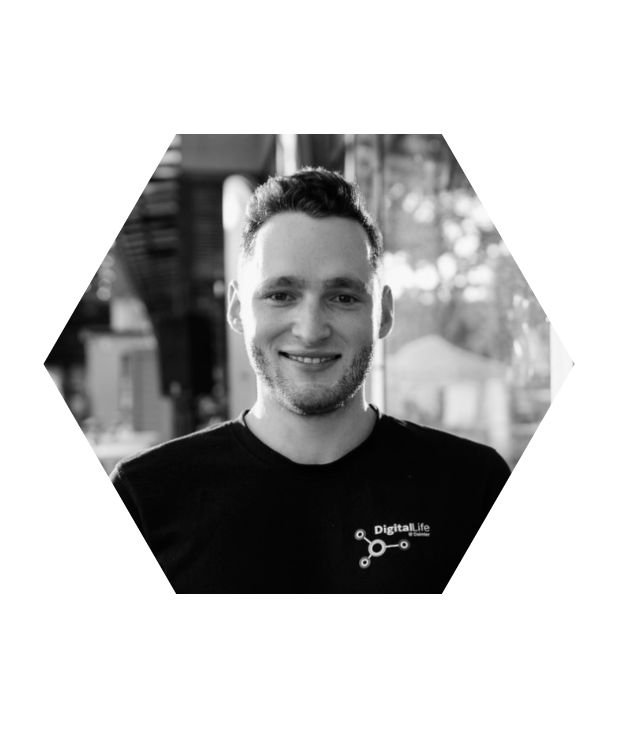
\includegraphics[width=\textwidth]{chapters/01_introduction/figures/me.png}
            \end{column}
            \begin{column}{0.6\textwidth}
                \begin{itemize}
                    \item Jonas Miederer
                	\item 27 Jahre
                	\item Hauptberuflich tätig bei der Daimler AG als Softwareentwickler für Künstliche Intelligenz
                	\item Studium an der Hochschule der Medien (Bachelor: Medieninformatik, Master: Computer Science And Media)
                	\item Bei Fragen, Problemen oder Unklarheiten gerne melden: \href{mailto:dhbw@jonas-miederer.de}{hello@jonas-miederer.de} oder \href{https://jonas-miederer.de/}{https://jonas-miederer.de/}
          	    \end{itemize}
            \end{column}
        \end{columns}
    \end{frame}
          
   \section{Über die Veranstaltung}  
     \begin{frame}{Inhalte}
        
        \begin{itemize}
            \item Grundlagen der Informatik
            \item Kernanwendungen und aktuelle Themen der Informatik
            \item Algorithmen, Programm- und Datenstrukturen
            \item Problemlösung mit modernen Programmier-/Skriptsprachen
            \item Datenbankverwaltung, -entwurf \& -implementierung
            \item Datenbankkonzepte
        \end{itemize}
    \end{frame}
    
    \begin{frame}{Ziele}
        \begin{itemize}
            \item Grundverständnis der Konzepte in der Informatik
            \item Lösungskompetenz unterschiedlicher Problemstellungen in der Informatik
            \item Implementierung eigener Algorithmen und Funktionalitäten
        \end{itemize}
    \end{frame}
    
    \begin{frame}{Termine}
        \textbf{Semester 1:}
        \begin{itemize}
            \item 27.11.2020
            \item 04.12.2020
            \item 11.12.2020
            \item 18.12.2020
            \item 08.01.2021
            \item 15.01.2021
            \item 22.01.2021
        \end{itemize}
        
        \textbf{Semester 2:}
        \begin{itemize}
            \item 14.05.2021 (Prüfungsvorbereitung)
        \end{itemize}
    \end{frame}
    
    \begin{frame}{Organisation \& Prüfungsleistung}
    
        \begin{itemize}
            \item Kombination aus Theorie \& Praxis
            \item Übungen zur Anwendung des Gelernten
            \item Workload 150 Stunden (74 Präsenz / 76 Selbststudium) \newline
            \item Prüfungsleistung: Programmentwurf
            \item 5 ECTS-Punkte
        \end{itemize}
     \end{frame}
    

%\newcommand{\decktitle}{Grundlagen der Informatik}
%%%%%%%%%%%%%%%%%%%%%%%%%%%%%%%%%%%%%%%%%%%%%%%%%
%
% DOCUMENT
%
%%%%%%%%%%%%%%%%%%%%%%%%%%%%%%%%%%%%%%%%%%%%%%%%%

\begin{frame}
    \subtitle{\decktitle}
    \titlepage
\end{frame}


\begin{frame}
    \frametitle{\textbf{Outline:}}
    \tableofcontents
\end{frame}


		
  
\section{Grundlagen der Informatik}  
    \subsection{Definition}
    
    \begin{frame}{Was ist Informatik?}
        \begin{definition}
         \begin{quote}
            Wissenschaft von der systematischen Darstellung, Speicherung, Verarbeitung und Übertragung von Informationen, besonders der automatischen Verarbeitung mithilfe von Digitalrechnern \cite{claus2006duden}
            \end{quote}  
        \end{definition}
        
    \end{frame}
          
    \begin{frame}{Was ist Informatik?}
        Informatik setzt sich als Kofferwort aus den zwei Bereichen \alert{Information} und \alert{Automatik} zusammen. 
        \\[2\baselineskip]
        
        Es geht also um \textit{automatisierte Informations- / Datenverarbeitung}. Beide Teilbereiche sind elementar wichtig und werden im Rahmen dieser Veranstaltung direkt und indirekt näher beleuchtet.
    \end{frame}
    
    \subsection{Teilbereiche der Informatik am Beispiel Google}
    
    \begin{frame}{Was ist Informatik?}
    \framesubtitle{Beispiel Google: Programmierung}
     \begin{columns}
        \begin{column}{0.5\textwidth}
            \begin{figure}
                \centering
                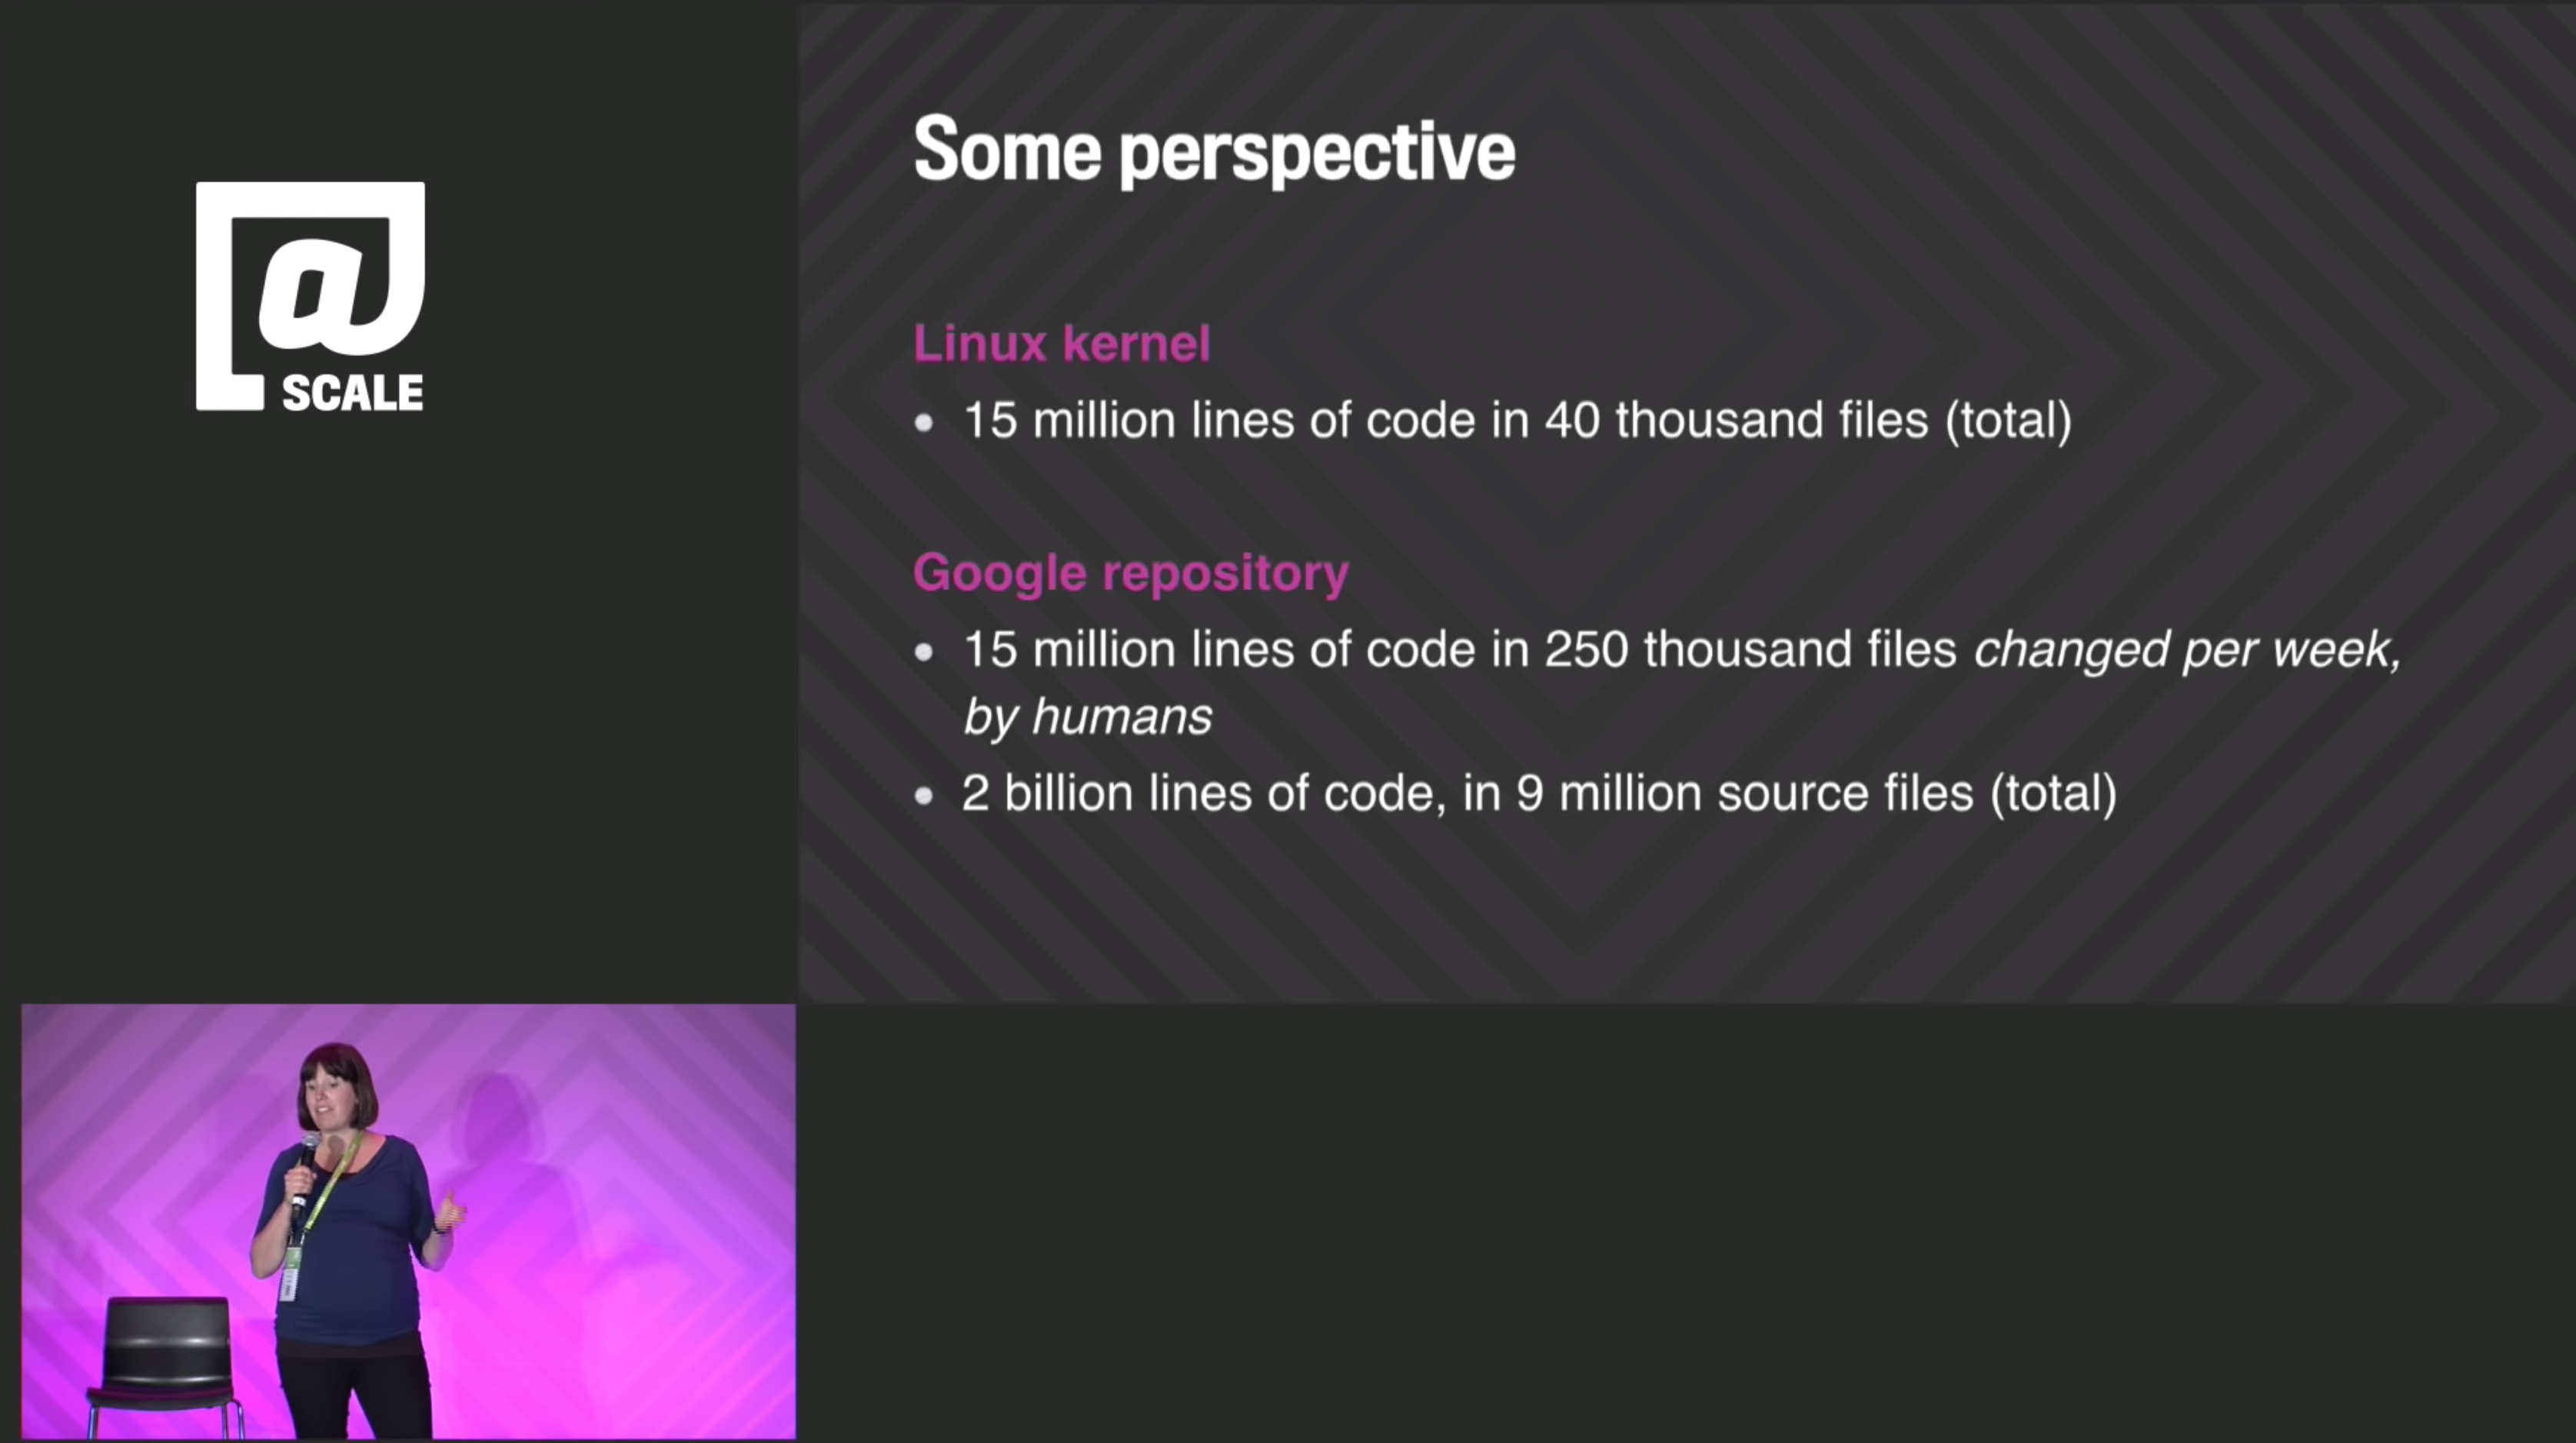
\includegraphics[width=\linewidth,height=0.6\textheight,keepaspectratio]{chapters/02_computer_science/figures/google/programming/loc.png}
                \caption{Größe der Google Codebasis \cite{google:potvin}}
                \label{fig:my_label}
            \end{figure}
        \end{column}
        \begin{column}{0.4\textwidth}
            \begin{figure}
            \centering
            \begin{subfigure}{0.475\textwidth}
                \centering
                
\includegraphics[width=\textwidth,height=0.15\textheight,keepaspectratio]{chapters/02_computer_science/figures/google/programming/languages/python.png}
            \end{subfigure}
            \begin{subfigure}{0.475\textwidth}
                \centering
                
\includegraphics[width=\textwidth,height=0.15\textheight,keepaspectratio]{chapters/02_computer_science/figures/google/programming/languages/cpp.png}
            \end{subfigure}
            
            \vskip\baselineskip
            
            \begin{subfigure}{0.475\textwidth}
                \centering
                
\includegraphics[width=\textwidth,height=0.15\textheight,keepaspectratio]{chapters/02_computer_science/figures/google/programming/languages/java.png}
            \end{subfigure}
            
             \begin{subfigure}{0.475\textwidth}
                \centering
                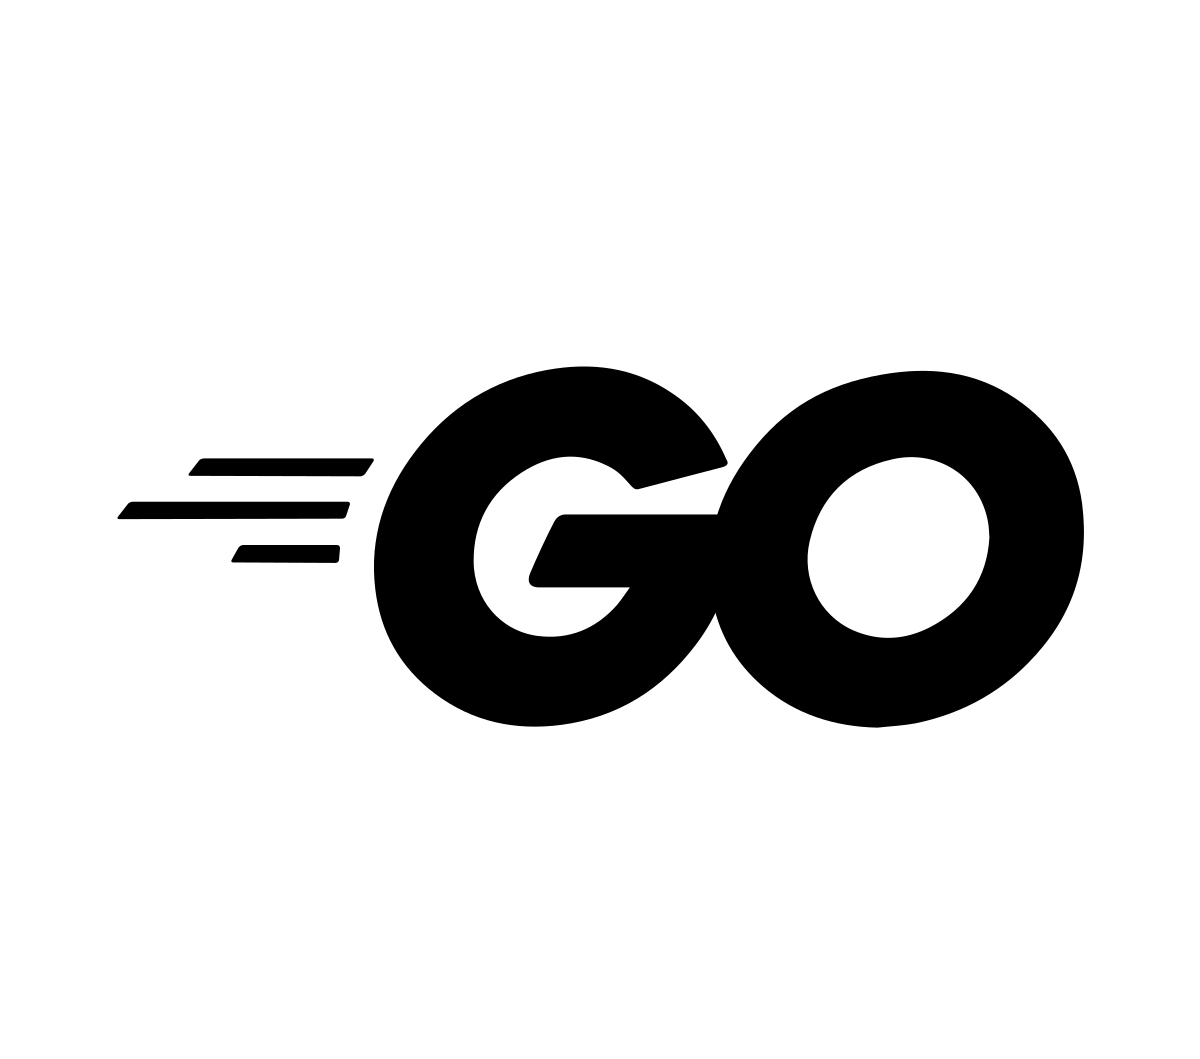
\includegraphics[width=\textwidth,height=0.15\textheight,keepaspectratio]{chapters/02_computer_science/figures/google/programming/languages/go.png}
            \end{subfigure}
            
            \caption{Hauptprogrammiersprachen von Google}
            \end{figure}
        \end{column}
    \end{columns}
    \end{frame}
    
    
    \begin{frame}[fragile]{Was ist Informatik?}
        \framesubtitle{Beispiel Google: Systems Design}
        \begin{figure}
            \centering
            
\includegraphics[width=\linewidth,height=0.3\textheight,keepaspectratio]{chapters/02_computer_science/figures/google/sys_des/searches.png}
            \caption{
                Google-Anfragen pro Jahr (2016, geschätzt) 
                \cite{google:sys_des:searches}
            }
        \end{figure}
        
        \begin{figure}
            \centering
            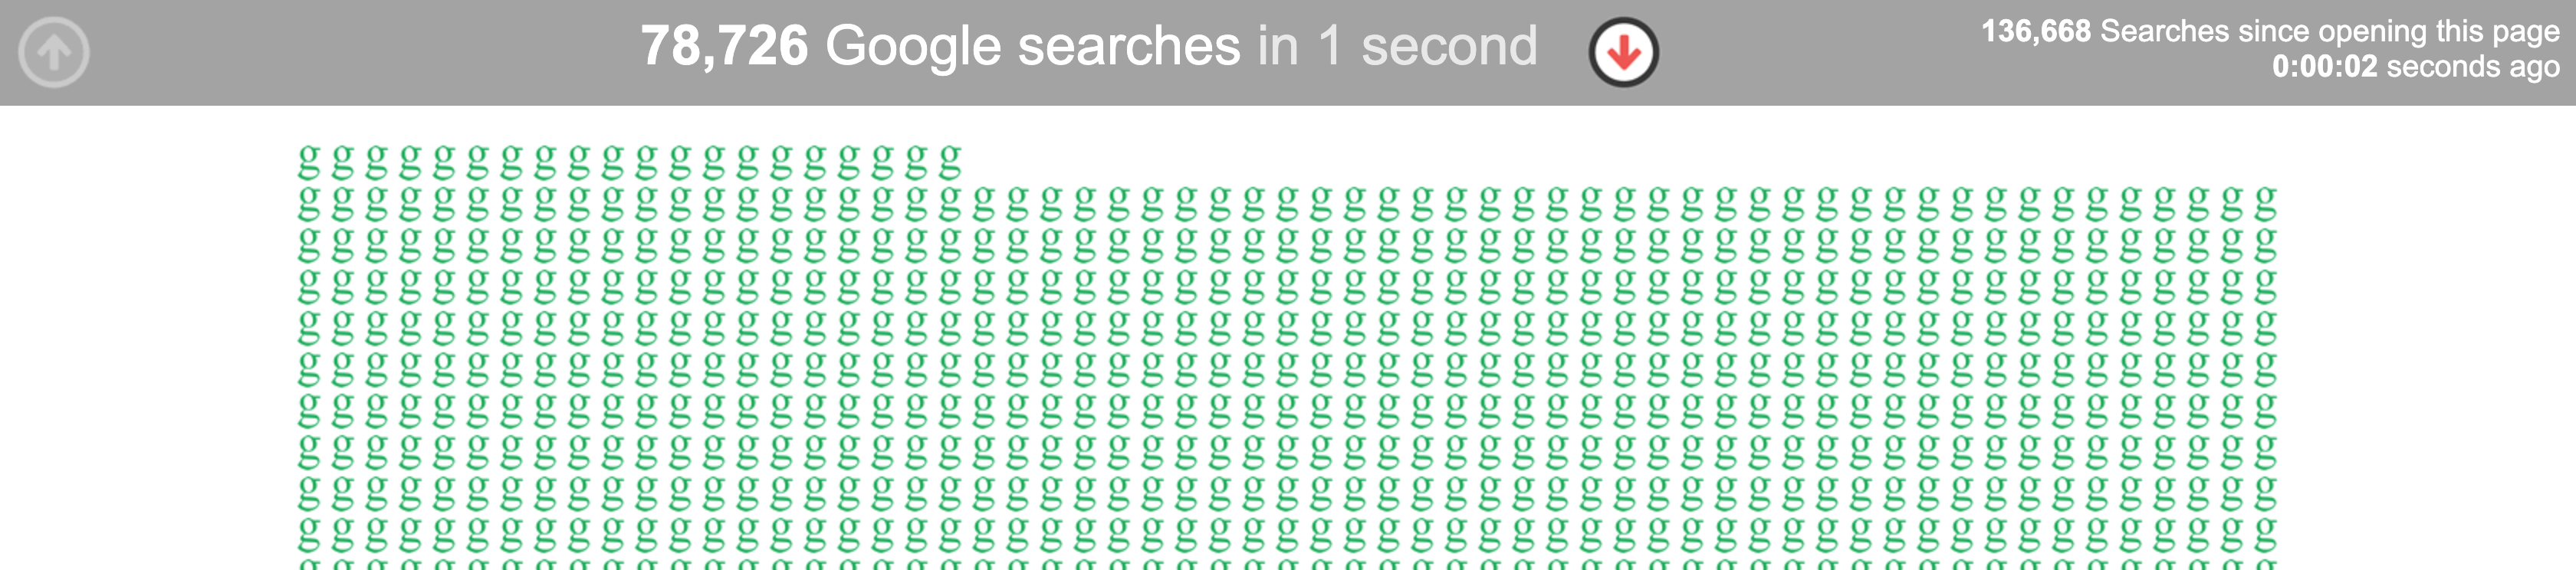
\includegraphics[width=\linewidth,height=0.3\textheight,keepaspectratio]{chapters/02_computer_science/figures/google/sys_des/searches2.png}
            \caption{
                \href{https://www.internetlivestats.com/one-second/#google-band}{Visualisierung der Anzahl der Google-Suchen pro Sekunde} (geschätzt)
            }
        \end{figure}
    
    \end{frame}
    
     \begin{frame}{Was ist Informatik?}
        \framesubtitle{Beispiel Google: Systems Engineering}
        \begin{figure}
            %\centering
            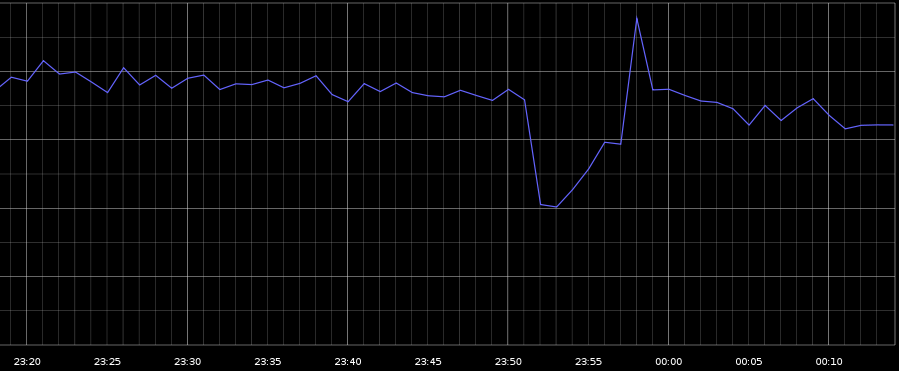
\includegraphics[width=\linewidth,height=0.3\textheight,keepaspectratio]{chapters/02_computer_science/figures/google/downtime/downtime.png}
            \caption{Einbruch des Internettraffics um 40\% während eines 2-minütigen Ausfalls von Google \cite{google:down:chart}}
            \label{fig:my_label}
        \end{figure}
        
         \begin{figure}
            %\centering
            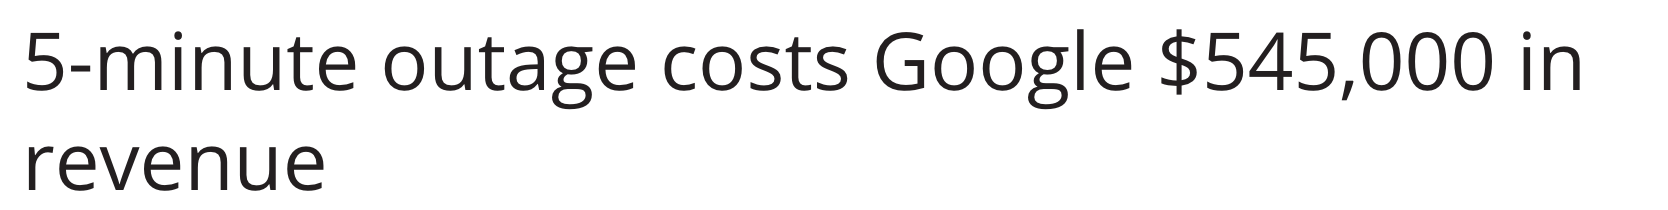
\includegraphics[width=0.4\linewidth,height=0.3\textheight,keepaspectratio]{chapters/02_computer_science/figures/google/downtime/costs.png}
            \caption{Geschätzte Kosten des Google-Ausfalls \cite{google:down:costs}}
            \label{fig:my_label}
        \end{figure}
    \end{frame}
    
    
    \begin{frame}{Was ist Informatik?}
        \framesubtitle{Beispiel Google: Algorithmik, Komplexitätsanalyse \& Mathematik}
        \begin{figure}
            \centering
            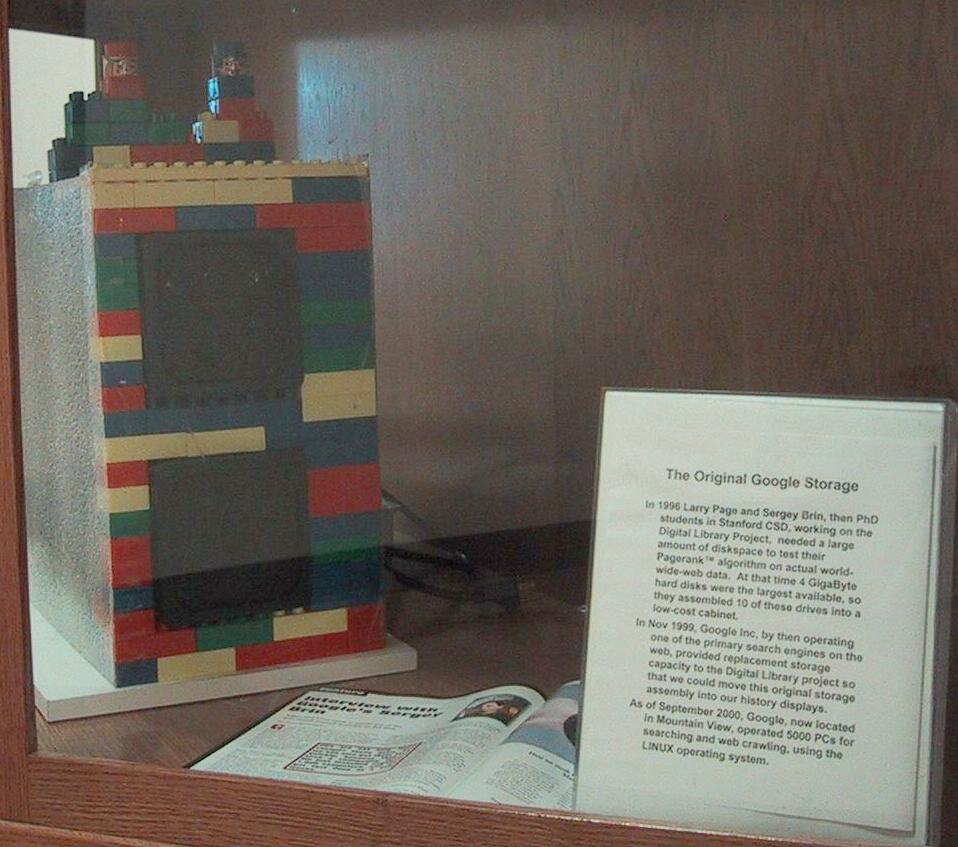
\includegraphics[width=\linewidth,height=0.6\textheight,keepaspectratio]{chapters/02_computer_science/figures/google/storage.jpg}
            \caption{Der erste Google-Computer mit 10x4 GB Harddrives \cite{google:alg:storage}}
            \label{fig:my_label}
        \end{figure}
      
    \end{frame}
    
    
    \begin{frame}{Was ist Informatik?}
        \framesubtitle{Beispiel Google: Algorithmik, Komplexitätsanalyse \& Mathematik}
        \begin{figure}
            \centering
            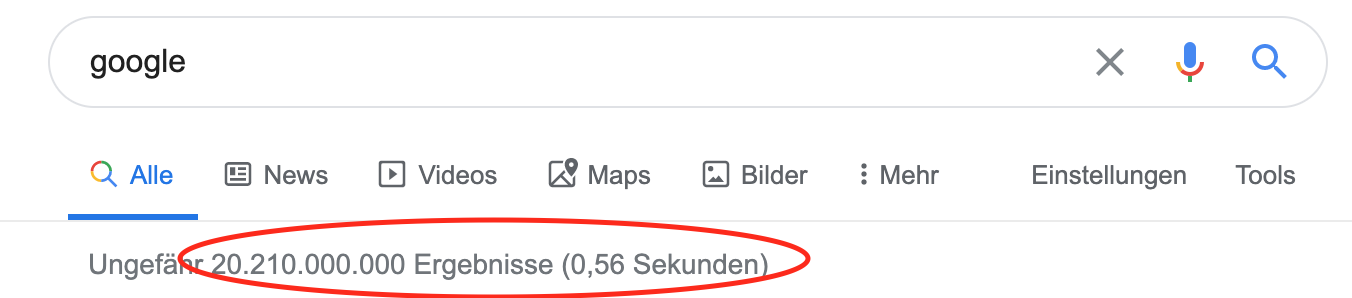
\includegraphics[width=\linewidth,height=0.6\textheight,keepaspectratio]{chapters/02_computer_science/figures/google/algorithms/results.png}
            \caption{Leistungsfähigkeit der Google-Suche}
            \label{fig:my_label}
        \end{figure}
        
        \begin{quote}
            "Der Google-Suchindex umfasst Milliarden von Webseiten und ist über 100.000.000 Gigabyte groß." \cite{google:alg:index}
        \end{quote}
    \end{frame}
    
    \begin{frame}{Was ist Informatik?}
        \framesubtitle{Beispiel Google: Systemarchitektur}
        \begin{figure}
            \centering
            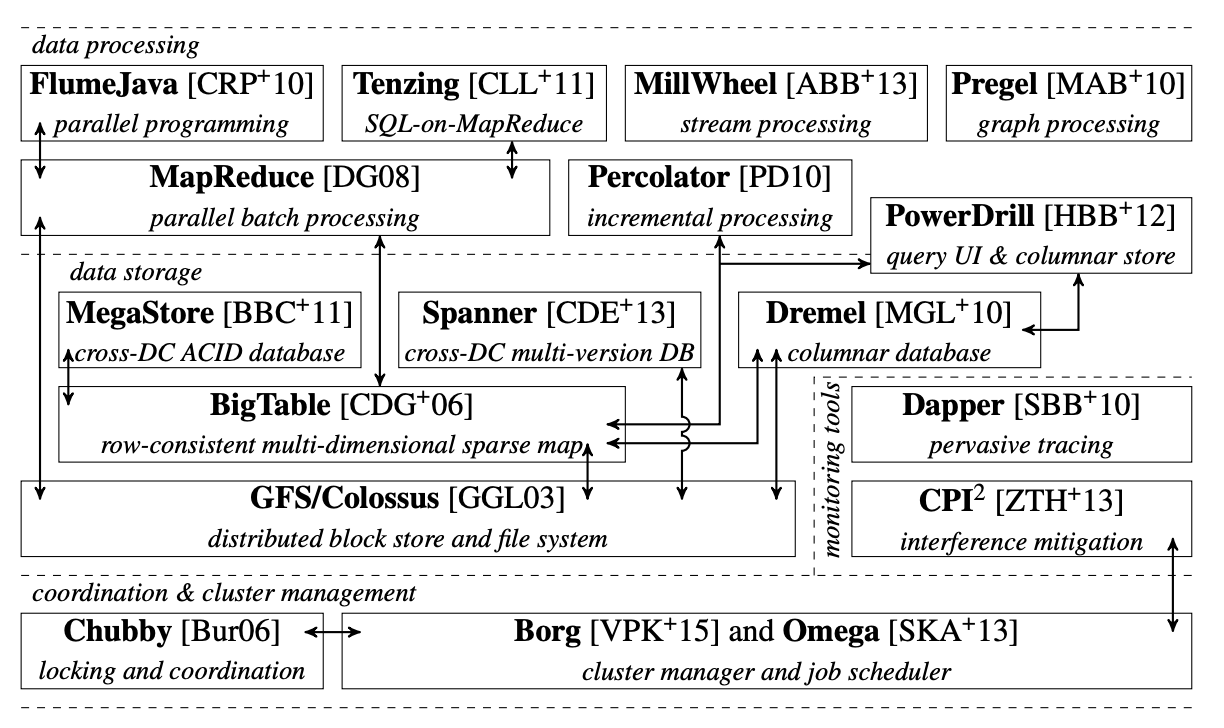
\includegraphics[width=\linewidth,height=0.6\textheight,keepaspectratio]{chapters/02_computer_science/figures/google/architecture/stack.png}
            \caption{Der Google Infrastruktur-Stack \cite{google:arch:stack}}
            \label{fig:my_label}
        \end{figure}
        
        
    \end{frame}
    
    
    \begin{frame}{Was ist Informatik?}
        \framesubtitle{Beispiel Google: Verteilte Systeme}
        \begin{figure}
            \centering
            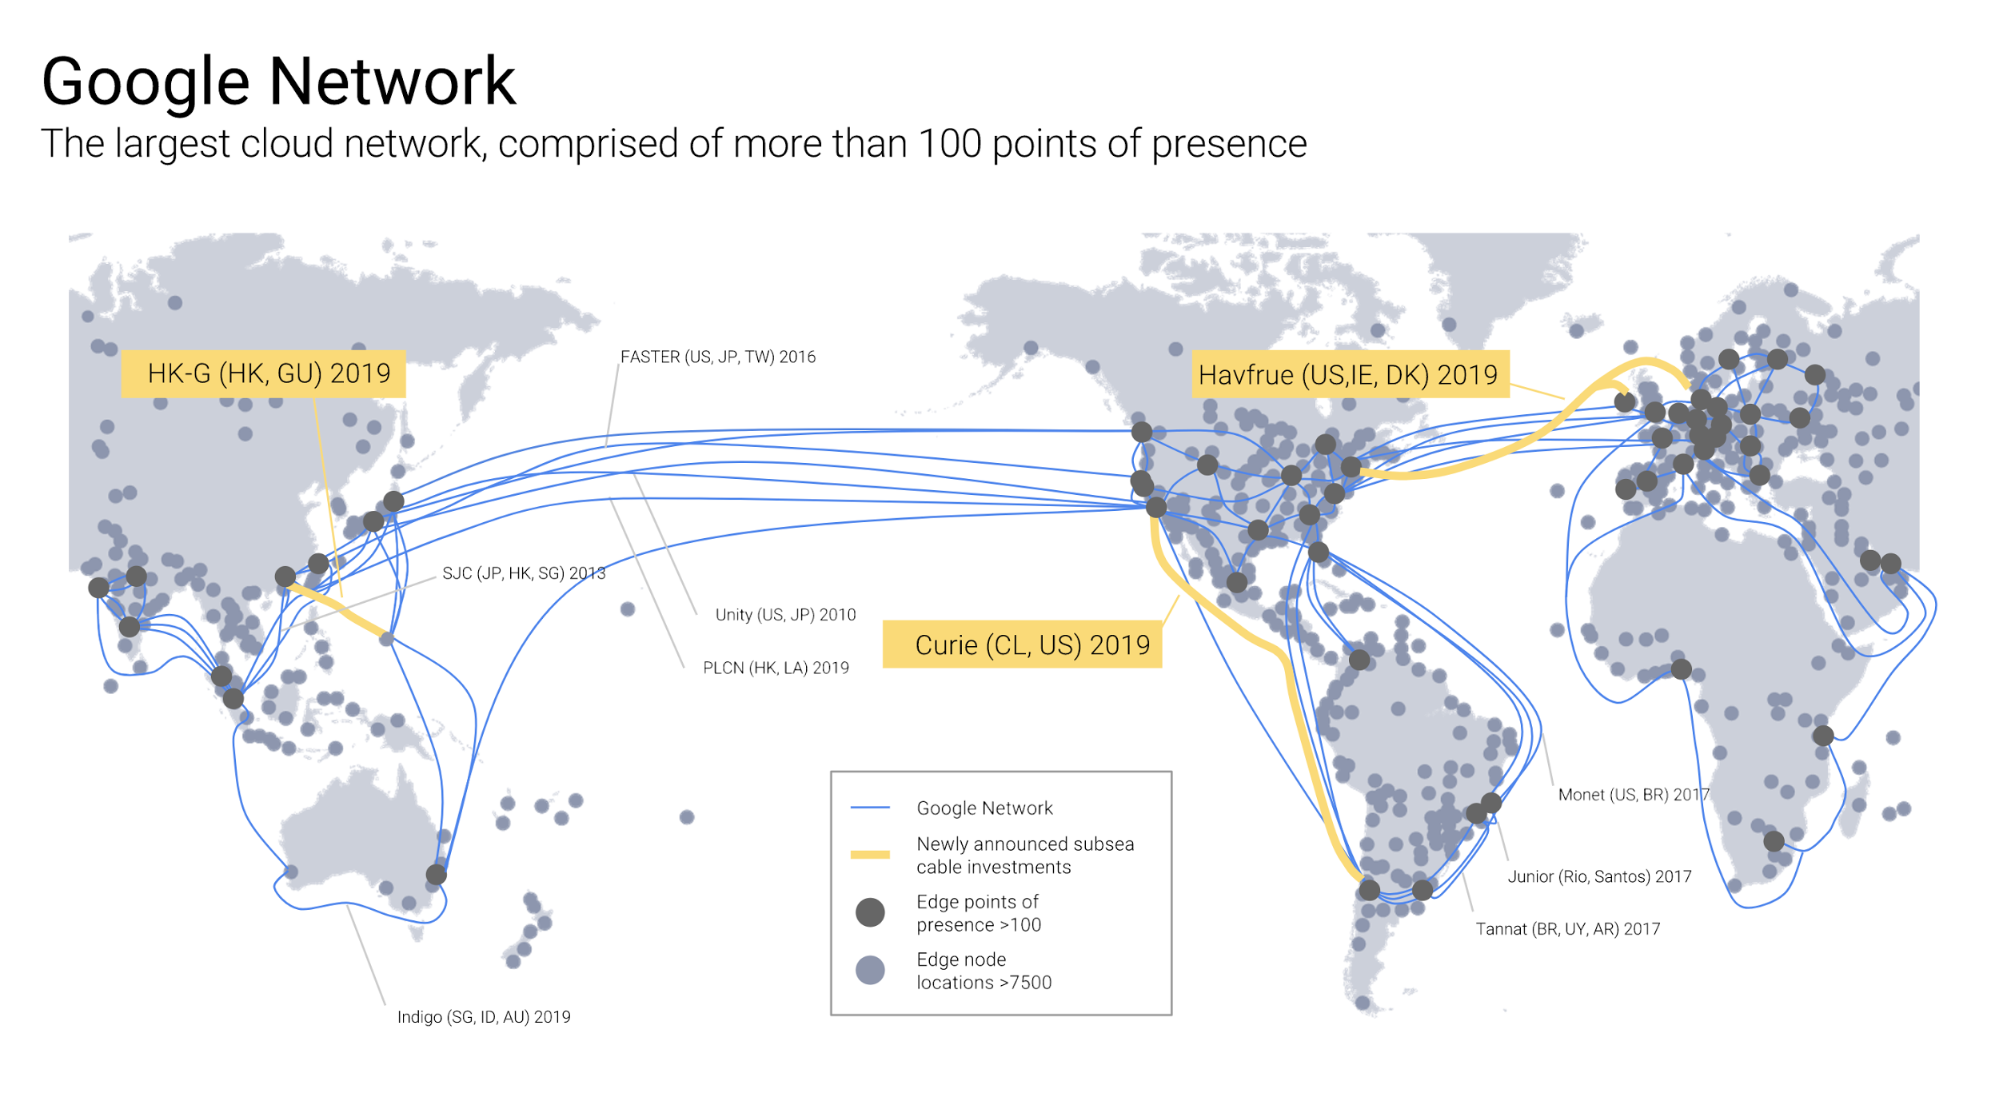
\includegraphics[width=\linewidth,height=0.3\textheight,keepaspectratio]{chapters/02_computer_science/figures/google/distributed/infrastructure.png}
            \caption{Globale Netzwerk-Infrastruktur der Google Cloud \cite{google:dist:infra}}
            \label{fig:my_label}
        \end{figure}
        
        \begin{figure}
            \centering
            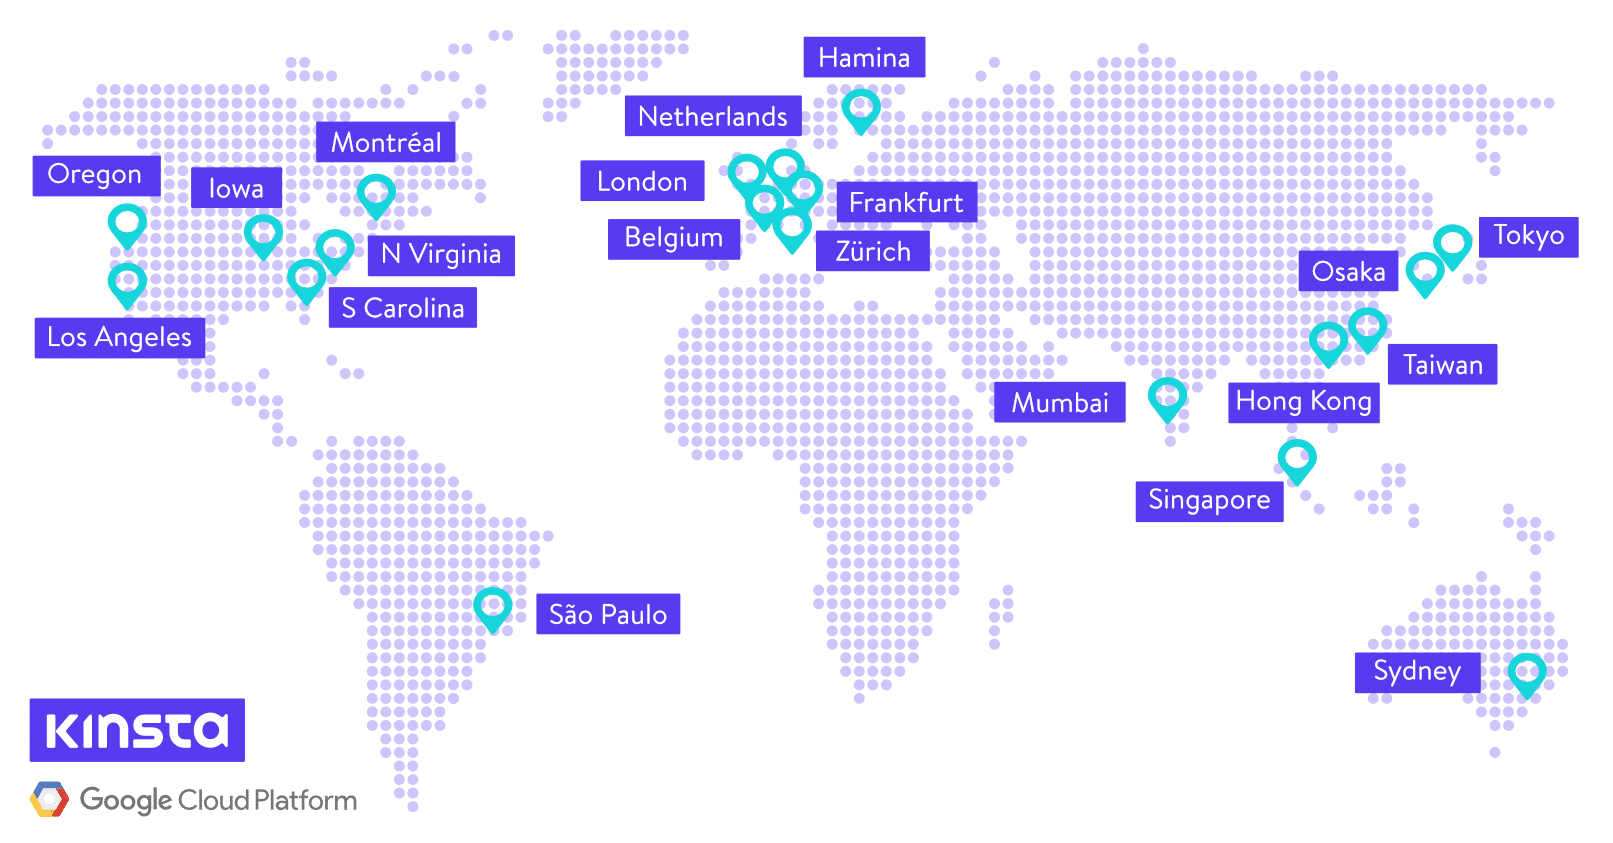
\includegraphics[width=\linewidth,height=0.3\textheight,keepaspectratio]{chapters/02_computer_science/figures/google/distributed/datacenter.png}
            \caption{Standorte der Google-Rechenzentren \cite{google:dist:datacenter}}
            \label{fig:my_label}
        \end{figure}
        
        
    \end{frame}

    \subsection{Disziplinen der Informatik} 
    
    \begin{frame}{Was ist Informatik?}
        \framesubtitle{Disziplinen der Informatik}
        Informatik besteht aus vielen Teildisziplinen, z.B.:
        \begin{itemize}
            \item Computerarchitektur
            \item Rechnernetze
            \item Compilerentwurf- und entwicklung
            \item Theoretische Informatik
            \item Verteilte Systeme
            \item Simulation \& Computergrafik
            \item Künstliche Intelligenz \& Machine Learning
            \item ...
        \end{itemize}
    \end{frame}
    
    \begin{frame}{Was ist Informatik?}
        \framesubtitle{Disziplinen der Informatik}
        \begin{figure}
            \centering
            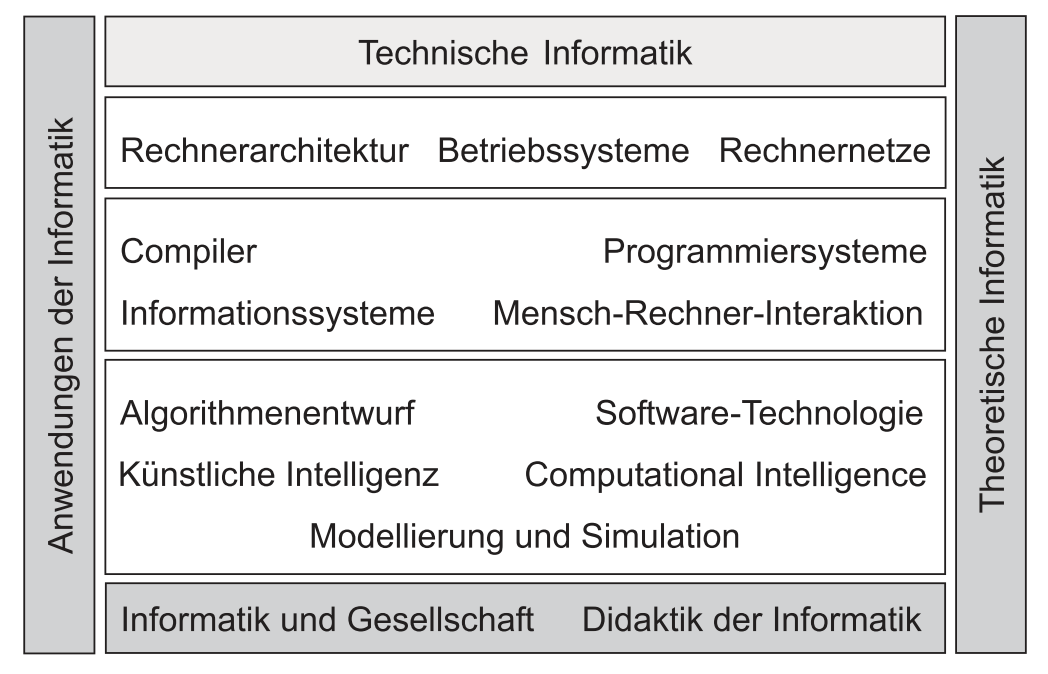
\includegraphics[width=\linewidth,height=0.6\textheight,keepaspectratio]{chapters/02_computer_science/figures/informatik_einordnung.png}
            \caption{Einordnung der Teilgebiete der Informatik \cite{Muller2015}}
            \label{fig:my_label}
        \end{figure}
    \end{frame}
        
    
%\newcommand{\decktitle}{Grundlagen der Programmierung}

%%%%%%%%%%%%%%%%%%%%%%%%%%%%%%%%%%%%%%%%%%%%%%%%%
%
% DOCUMENT
%
%%%%%%%%%%%%%%%%%%%%%%%%%%%%%%%%%%%%%%%%%%%%%%%%%

\begin{frame}
    \subtitle{\decktitle}
    \titlepage
\end{frame}


\begin{frame}
    \frametitle{\textbf{Outline:}}
    \tableofcontents
\end{frame}

		
		
		
  
\section{Programmierung: Begriffsabgrenzung}  

  \begin{frame}{Programmierung: Definition}
        \label{def:programming}
        \begin{definition}
            "Vorgang der Erstellung eines Programms durch den Programmierer. Bei Verwendung einer prozeduralen Programmiersprache umfasst Programmentwicklung:\newline
    (1) die Entwicklung des Algorithmus und der Datenvereinbarungen;\newline
    (2) deren Umsetzung mit den Ausdrucksmitteln einer Programmiersprache (Codierung)." \cite{gabler:programmierung}
        \end{definition}
    \end{frame}
    
    \begin{frame}{Programmierung: Einordnung des Begriffs}
        Die Programmierung besteht laut dieser Definition also aus 2 Teilbereichen:
        
        \begin{itemize}
            \item \textbf{Beschreibung durch Programmiersprache:} Beschreibt den Aufbau und die Funktionalität eines Programms in \textit{formaler} Hinsicht
            \item \textbf{Algorithmus und Datenvereinbarungen:} Beschreibt den Aufbau und die Funktionalität eines Programms in \textit{logischer} Hinsicht
        \end{itemize}
        
        Die Beschreibung der Funktionalität eines Programms ist stets auch ohne der Verwendung einer Programmiersprache möglich. Um diese Funktionalitäten jedoch vom Computer ausführen zu lassen ist eine Codierung der Anweisungen in eine der Programmiersprachen nötig.
    \end{frame}
    
    
    \begin{frame}{Programmierung: Einordnung des Begriffs}
    
        Obwohl Programmierung häufig als Synonym für die Informatik genutzt wird, handelt es sich dabei lediglich um eine von vielen Disziplinen innerhalb der Informationsverarbeitung. Oftmals sind Grundkenntnisse in der Programmierung notwendig, um andere Teilbereiche der Informatik beherrschen zu können. 
    \end{frame}
    
     \begin{frame}{Programmierung vs. Softwareentwicklung}
    
        \begin{itemize}
            \item Programmierung und Softwareentwicklung werden häufig als Synonyme genutzt
            \item Programmierung beschreibt lediglich die (tatsächliche) Erstellung eines Programms (siehe S. \ref{def:programming})
            \item Softwareentwicklung beschreibt den kompletten Prozess von der Architektur (wie ist das Programm aufgebaut) über die Implementierung bis hin zur Verprobung und Inbetriebnahme einer Software
            \item Im holistischen Ansatz der Softwareentwicklung ist Programmierung also nur ein Teilbereich 
            \item Ziel der Veranstaltung: Nicht nur Programmierkenntnisse, sondern auch Fähigkeiten in diversen Themen der Softwareentwicklung (Planung und Entwurf von Programmen, Komplexitätsanalyse, ...)
            
        \end{itemize}
    \end{frame}
 

\section{Überblick: Von der Rechnerarchitektur zur Programmiersprache}

    \begin{frame}{Aufbau eines Rechensystems}
    
    \begin{figure}
        \centering
        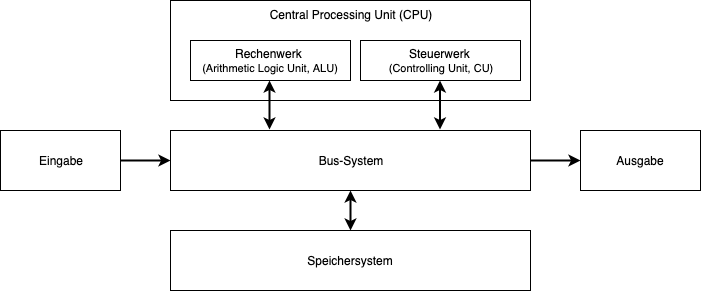
\includegraphics[width=\linewidth,height=0.45\textheight,keepaspectratio]{chapters/03_programming/figures/von_neumann.png}
        \caption{Schematische Darstellung der Von-Neumann-Architektur}
        \label{fig:von_neumann}
    \end{figure}
    
    Die Von-Neumann-Architektur ist eine abstrakte Beschreibung, nach der annähernd alle Rechensysteme aufgebaut sind. Sie besteht aus 5 grundlegenden Komponenten: Ein- und Ausgabe von Daten, Speicherwerk zum (flüchtigen oder persistenten) Speichern der Daten, der zentralen Recheneinheit (CPU) mit der Steuereinheit (CU) und dem Rechenwerk (ALU) sowie dem Bus-System, das die Kommunikation und den Datenaustausch zwischen den Komponenten ermöglicht.
    
    \end{frame}
        
    
    
    \begin{frame}{Vom Programmcode zur Ausführung}
        \begin{columns}
            \begin{column}{0.4\textwidth}
                \begin{figure}
                    \centering
                    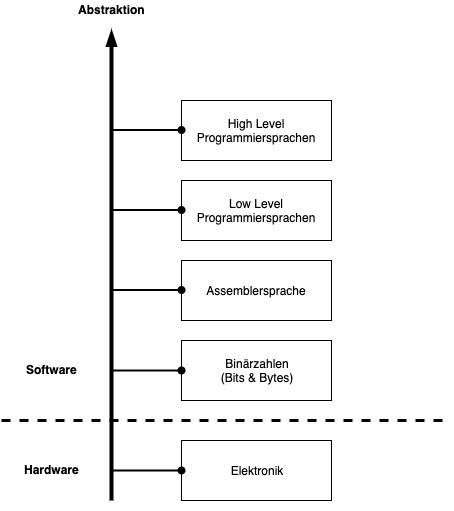
\includegraphics[width=\linewidth,height=0.6\textheight,keepaspectratio]{chapters/02_computer_science/figures/Abstraction.png}
                    \caption{Abstraktionsgrade}
                    \label{fig:abstraction}
                \end{figure}
            \end{column}
            \begin{column}{0.6\textwidth}
                \begin{itemize}
                    \item Der Mensch gibt dem Computer Anweisungen, die ausgeführt werden sollen
                	\item Diese Kommunikation kann auf mehr oder weniger abstrakter Ebene ablaufen
                	\item Eine Abstraktion weg vom spezifischen Funktionsprinzip eines Computers hin zur natürlichen Sprache des Menschen kann die Entwicklung erleichtern
          	    \end{itemize}
            \end{column}
        \end{columns}
    \end{frame}
    

\begin{frame}{Vom Programmcode zur Ausführung}
        \begin{itemize}
            \item Zwischen den Anweisungen, die dem System in Form von Programmcode übermittelt wird, und der eigentlichen Ausführung dieser Anweisungen liegen mehrere Schritte, um den Code in eine für den Computer verarbeitbare Form zu bringen.
            \item Hierbei wird zwischen \alert{Kompilierung} und \alert{Interpretierung} unterschieden (siehe Abb. \ref{fig:compilation_interpretation}).
            \item Die beiden Ansätze können auch in Form von JIT\footnote{Just in Time}-Kompilierung kombiniert werden.
        \end{itemize}
         
        
        \begin{figure}
            \centering
            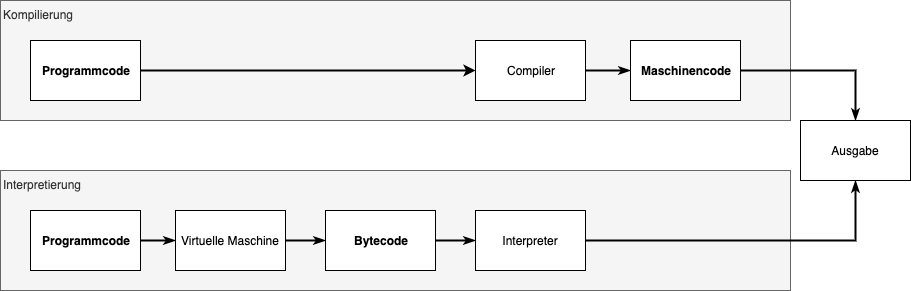
\includegraphics[width=\linewidth,height=0.3\textheight,keepaspectratio]{chapters/02_computer_science/figures/CompilationVSInterpretation.png}
            \caption{Kompilierung und Interpretierung}
            \label{fig:compilation_interpretation}
        \end{figure}
    \end{frame}

    
    
    
    \lstset{frame=tb,
  aboveskip=2mm,
  belowskip=12mm,
  showstringspaces=false,
  columns=flexible,
  basicstyle={\small\ttfamily},
  numbers=none,
  numberstyle=\tiny\color{gray},
  keywordstyle=\color{blue},
  commentstyle=\color{dkgreen},
  stringstyle=\color{mauve},
  breaklines=true,
  breakatwhitespace=true,
  tabsize=2
}
    
    \begin{frame}{Vom Programmcode zur Ausführung}
    
        \begin{example}
            Ausgabe von "Hello, World!"{} in \alert{\textit{Assembler}} (links), der systemnahen Programmiersprache \alert{\textit{C}} (mitte) und der höheren Programmiersprache \alert{\textit{Python}} (rechts)
        \end{example}
        
        
        \begin{columns}[T]
            \begin{column}{0.3\textwidth}
              \lstinputlisting[basicstyle=\tiny,language={[x86masm]Assembler}]{chapters/02_computer_science/code/hello_world.asm}
            \end{column}
            
            \pause
            
            \begin{column}{0.3\textwidth}
              \lstinputlisting[basicstyle=\tiny,language=C]{chapters/02_computer_science/code/hello_world.c}
            \end{column}
            
            \pause
            \begin{column}{0.3\textwidth}
              \lstinputlisting[basicstyle=\tiny,language=Python]{chapters/02_computer_science/code/hello_world.py}
            \end{column}
        \end{columns}
        
    \end{frame}
  
  %\section{Moderne Programmiersprachen}
%\newcommand{\decktitle}{Programmiersprachen}

%%%%%%%%%%%%%%%%%%%%%%%%%%%%%%%%%%%%%%%%%%%%%%%%%
%
% DOCUMENT
%
%%%%%%%%%%%%%%%%%%%%%%%%%%%%%%%%%%%%%%%%%%%%%%%%%

\begin{frame}
    \subtitle{\decktitle}
    \titlepage
\end{frame}


\begin{frame}
    \frametitle{\textbf{Outline:}}
    \tableofcontents
\end{frame}

		
		
\section{Zweck von Programmiersprachen}		
    \begin{frame}{Programmiersprachen}
        Mithilfe von Computerprogrammen können komplexe wohldefinierte Problemstellungen (teil)automatisiert gelöst werden. Voraussetzung dafür ist, dass
        \begin{itemize}
            \item das Problem konkret beschrieben werden kann
            \item sich das Problem ihm Rahmen der Möglichkeiten einer Programmiersprache abbilden lässt
            \item es mindestens einen Lösungsweg gibt
            \item der Lösungsweg endlich ist
        \end{itemize}
    \end{frame}  
    
    \begin{frame}{Einordnung von Programmiersprachen}
        \begin{figure}
            \centering
            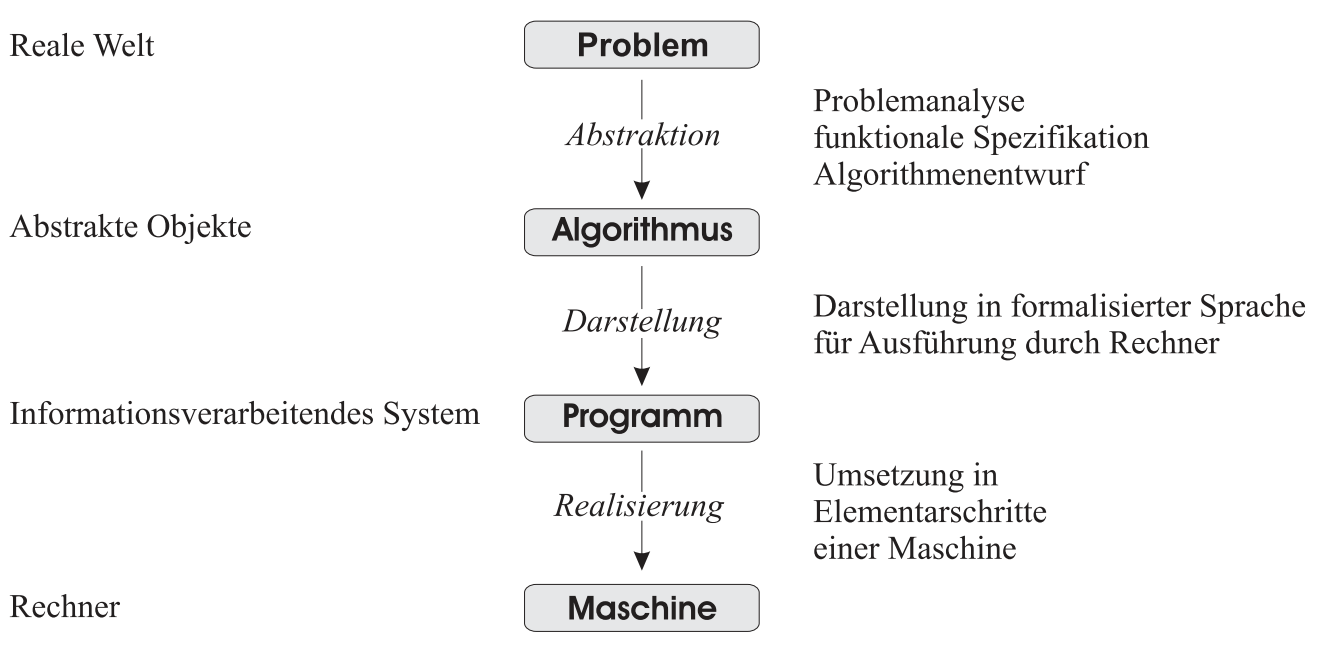
\includegraphics[width=\linewidth,height=0.5\textheight,keepaspectratio]{chapters/04_programming_languages/figures/problem2solution.png}
            \caption{Vorgehensweise zur Lösung von Problemen in der Informatik \cite{Muller2015}}
        \end{figure}
    \end{frame}
    
    \begin{frame}{Einordnung von Programmiersprachen}
        \begin{figure}
            \centering
            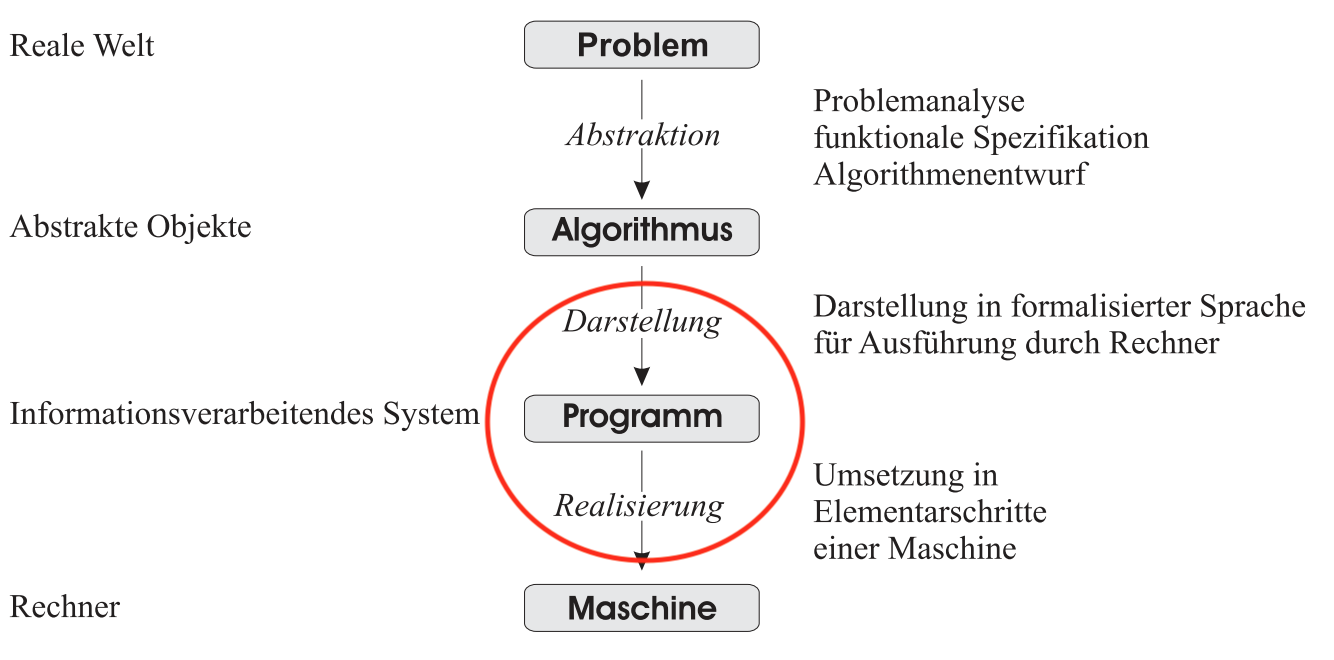
\includegraphics[width=\linewidth,height=0.5\textheight,keepaspectratio]{chapters/04_programming_languages/figures/problem2solution_marked.png}
            \caption{Vorgehensweise zur Lösung von Problemen in der Informatik \cite{Muller2015} (bearbeitet)}
        \end{figure}
    \end{frame}
    
    \begin{frame}{Zweck von Programmiersprachen}
        Programmiersprachen helfen also dabei, das Problem, welches zunächst abstrakt beschrieben wird, formal darzustellen und in eine Form zu übertragen, die für das Computersystem verarbeitbar ist.
    \end{frame}
    
    \begin{frame}{Einordnung von Programmiersprachen}
        \begin{figure}
            \centering
            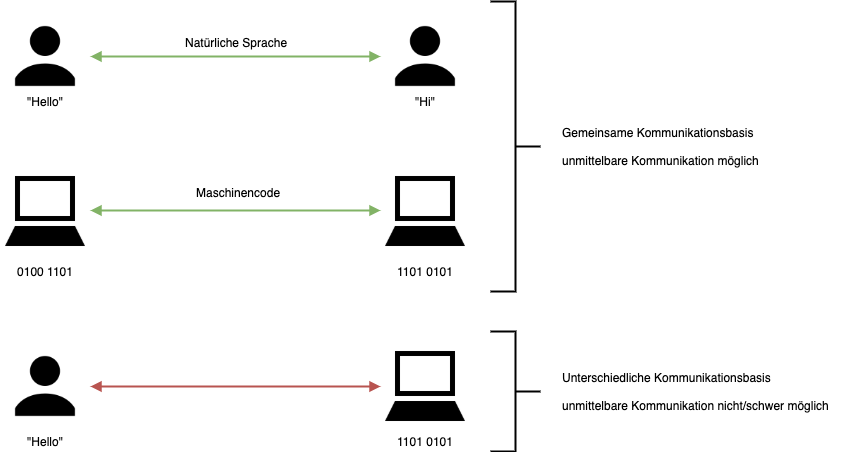
\includegraphics[width=\linewidth,height=0.5\textheight,keepaspectratio]{chapters/04_programming_languages/figures/communication_direct.png}
            \caption{Kommunikationswege zwischen Mensch und Computer (I)}
        \end{figure}
    \end{frame}
    
    \begin{frame}{Einordnung von Programmiersprachen}
        \begin{figure}
            \centering
            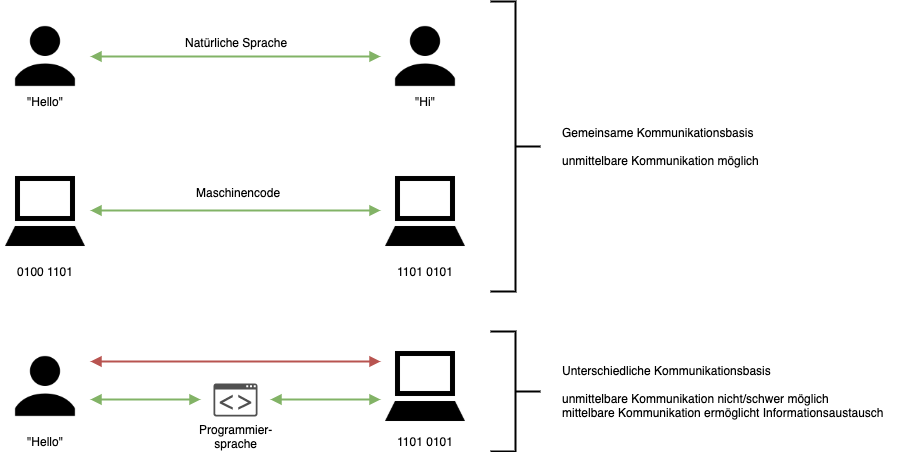
\includegraphics[width=\linewidth,height=0.5\textheight,keepaspectratio]{chapters/04_programming_languages/figures/communication_indirect.png}
            \caption{Kommunikationswege zwischen Mensch und Computer (II)}
        \end{figure}
    \end{frame}
    
\section{Vielfalt der Programmiersprachen}  

    \begin{frame}{Programmiersprachen}
        \begin{figure}
            \centering
            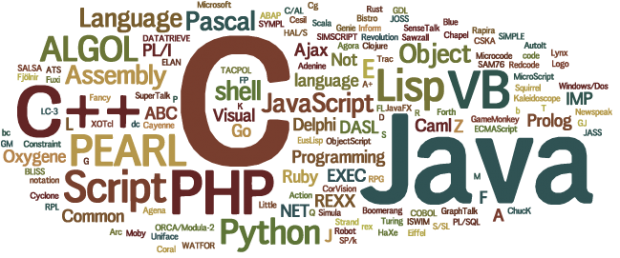
\includegraphics[width=\linewidth,height=0.5\textheight,keepaspectratio]{chapters/04_programming_languages/figures/languages.png}
            \caption{Word-Cloud zur Vielfalt an Programmiersprachen \cite{fig:programming_languages}}
        \end{figure}
    \end{frame}
    
    \begin{frame}{Beliebtheit von Programmiersprachen}
        \begin{figure}
            \centering
            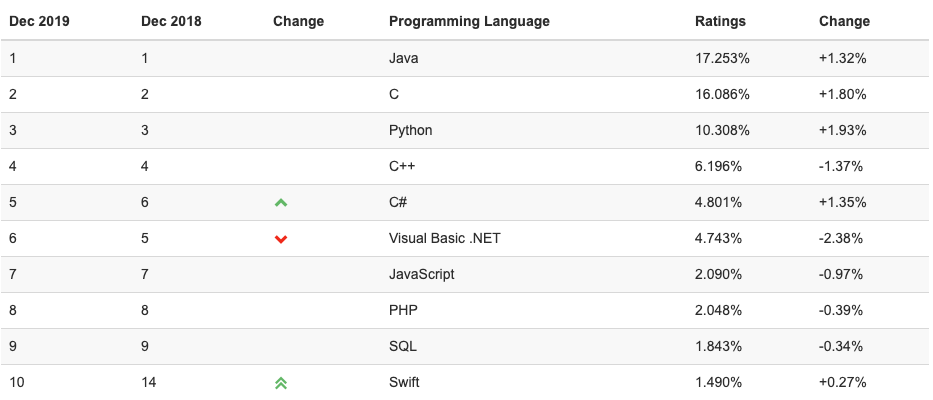
\includegraphics[width=\linewidth,height=0.5\textheight,keepaspectratio]{chapters/04_programming_languages/figures/tiobe_2019.png}
            \caption{TIOBE-Index zur Beliebtheit von Programmiersprachen 12/2019 \cite{fig:tiobe2019}}
        \end{figure}
        
        \begin{alertblock}{Hinweis}
        Der TIOBE-Index stellt keine wissenschaftliche Auswertung zur Beliebtheit von Programmiersprachen dar, die Ergebnisse sind lediglich auf Auswertungen von Suchanfragen gestützt. Dennoch bietet der Index einen groben Überblick.
        \end{alertblock}
    \end{frame}
    
    \begin{frame}{Beliebtheit von Programmiersprachen}
        \begin{figure}
            \centering
            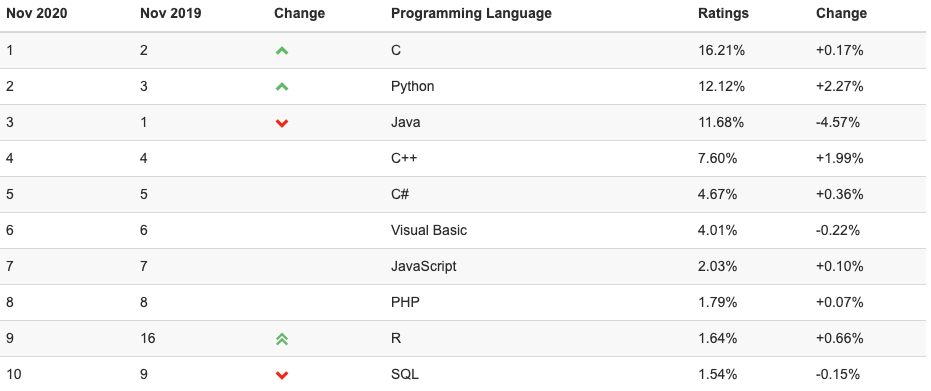
\includegraphics[width=\linewidth,height=0.5\textheight,keepaspectratio]{chapters/04_programming_languages/figures/tiobe_2020.png}
            \caption{TIOBE-Index zur Beliebtheit von Programmiersprachen 11/2020 \cite{fig:tiobe2019}}
        \end{figure}
        
    \end{frame}
    
    \begin{frame}{Beliebtheit von Programmiersprachen}
        \begin{figure}
            \centering
            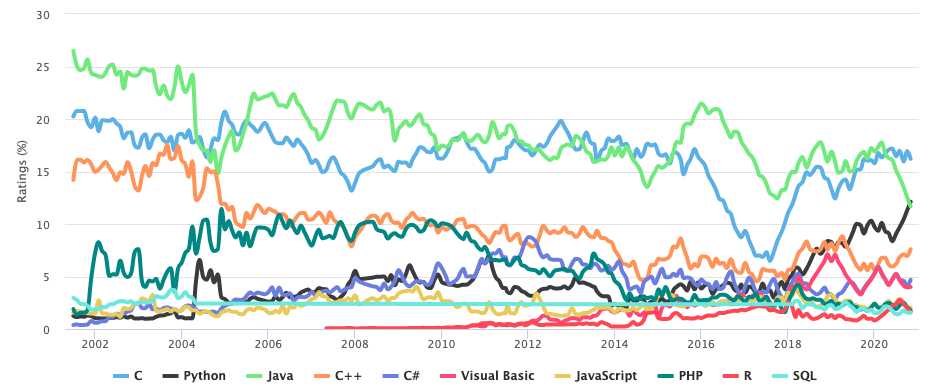
\includegraphics[width=\linewidth,height=0.5\textheight,keepaspectratio]{chapters/04_programming_languages/figures/tiobe_2002-2020.png}
            \caption{TIOBE-Index zur Beliebtheit von Programmiersprachen Juli 2001 - November 2020 \cite{fig:tiobe2001-2019}}
        \end{figure}
    \end{frame}
  
    \begin{frame}{Vielfältigkeit und Anzahl von Programmiersprachen}
        \begin{figure}
            \centering
            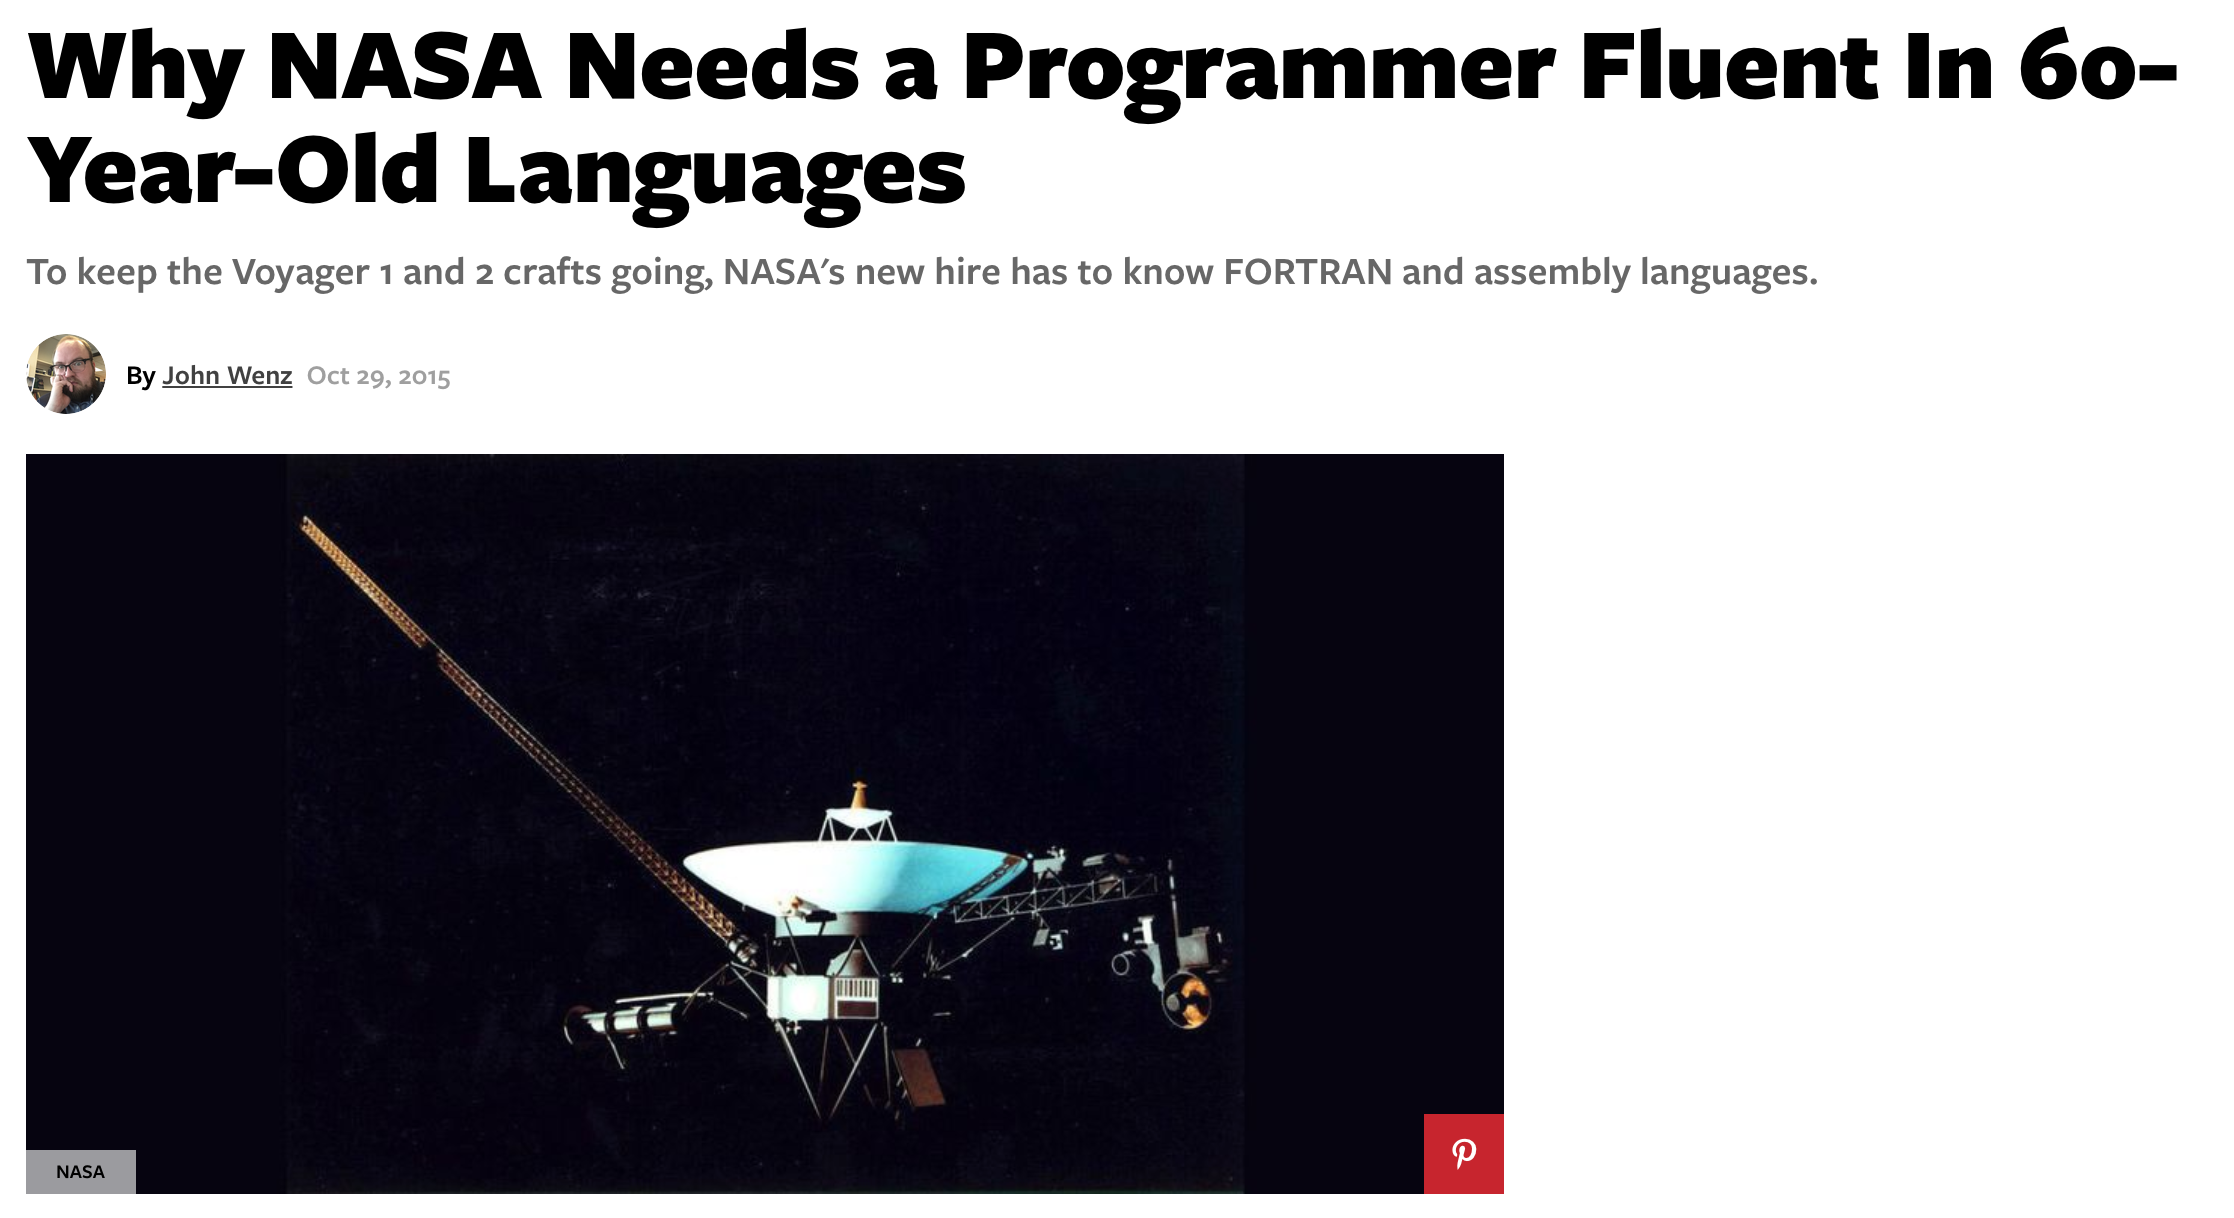
\includegraphics[width=\linewidth,height=0.5\textheight,keepaspectratio]{chapters/04_programming_languages/figures/voyager.png}
            \caption{Bericht über die Suche der NASA nach einem COBOL-Entwickler \cite{fig:voyager}}
            
        \note{
        1960er Jahre \\
        Fortran, Cobol, Assembler \\
        Radio-Übertragung, 17 Stunden
        }
        \end{figure}
        
    \end{frame}
    
    \begin{frame}{Frage 1: Was hat das mit Programmiersprachen zu tun?}
         \lstinputlisting[basicstyle=\tiny]{chapters/04_programming_languages/code/hello_world.spl}
    \end{frame}
    
    \begin{frame}{Frage 2: Was hat das mit Programmiersprachen zu tun?}
         \lstinputlisting[basicstyle=\tiny]{chapters/04_programming_languages/code/hello_world.tr}
    \end{frame}
    
    \begin{frame}{Frage 3: Was hat das mit Programmiersprachen zu tun?}
         \begin{figure}
            \centering
            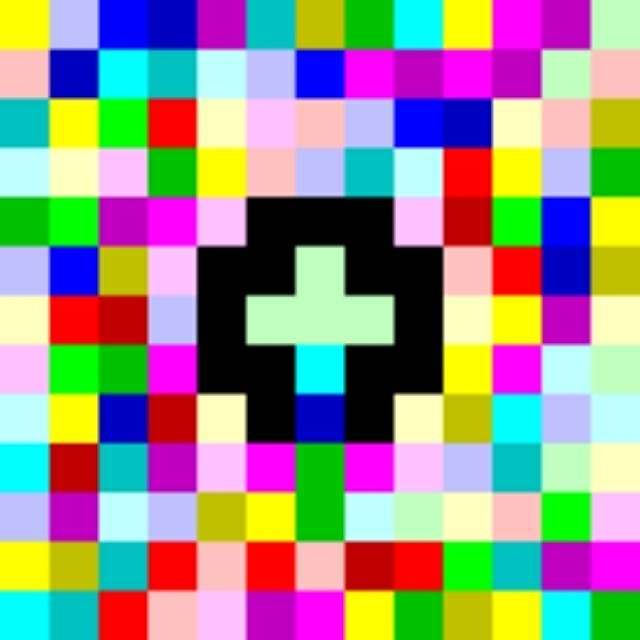
\includegraphics[width=\linewidth,height=0.5\textheight,keepaspectratio]{chapters/04_programming_languages/figures/hello_world_piet.jpg}
            \caption{\cite{fig:hello_world_piet}}
        \end{figure}
    \end{frame}
    
    \begin{frame}{Frage 4: Was hat das mit Programmiersprachen zu tun?}
         \lstinputlisting[basicstyle=\tiny]{chapters/04_programming_languages/code/hello_world.bf}
    \end{frame}
    
    
\section{Eigenschaften von Programmiersprachen (Gemeinsamkeiten)}
    \label{sec:properties}
    
    \begin{frame}{Eigenschaften}
        Alle Programmiersprachen müssen verschiedene Voraussetzungen erfüllen, damit es sich tatsächlich um eine Programmiersprache handelt. 
        
        \begin{alertblock}{Hinweis}
            Die im Folgenden aufgeführten Eigenschaften stellen lediglich die "Mindestvoraussetzungen" von Programmiersprachen dar. Die Programmiersprachen besitzen darüber hinaus noch viele weitere Eigenschaften, die sich jedoch unterscheiden können bzw. nicht zwingend in jeder Programmiersprache vorhanden sein müssen.
        \end{alertblock}
    \end{frame}
     
    \begin{frame}{Eingabe \& Ausgabe}
        Jede Programmiersprache muss \textbf{Eingaben} verarbeiten können (Informationsquelle). Dabei spielt es keine Rolle, ob die Eingabe durch eine manuelle Nutzereingabe (z.B. Text durch Tastatur/Maus, Spracheingabe, Dokumentenscan, ...) oder durch automatisiertes Einlesen von Daten (z.B. Datenbank, Datei, Programmierschnittstelle, ...)  erfolgt. \\~\
        
        Ebenso muss die \textbf{Ausgabe} von Informationen möglich sein, um dem Nutzer oder einem anderen System die Ergebnisse zur Verfügung zu stellen (Informationssenke). Auch hierfür gibt es genauso wie bei der Eingabe verschiedene Möglichkeiten (z.B. Ausgabe am Bildschirm, Audioausgabe, Datenbank, ...)  \\~\
        
        Auf welche Art und Weise und in welchem Format die Ein- und Ausgabe erfolgt ist jeweils abhängig vom Anwendungsfall und der Umsetzung im Programm und ist daher nicht vorgegeben.
        
        \note{
        Eingabe: Quelle, verschiedene Quellen \\
        Ausgabe: Ziel / Senke, verschiedene Ziele \\
        
        z.B. Sprachassistenten, Touchscreen, ... \\
        Quelle / Ziel abhängig von Implementierung
        }
    \end{frame}
    
    
    \begin{frame}{Deklaration von Variablen}
        Um Informationen innerhalb eines Programms verarbeiten zu können, müssen die Daten während der Verarbeitung zwischengespeichert werden. Hierzu werden Variablen genutzt, um Informationen referenzieren (darauf zugreifen) zu können. \\~\
        
        \begin{block}{Variable}
            Speichereinheit zur Aufnahme, Zwischenspeicherung und Modifikation von Daten(werten)
        \end{block}
        
        \begin{block}{Deklaration}
            Zuweisung / Zuordnung eines bestimmten Werts zu einer bestimmten Variablen (zu einem bestimmten Variablennamen)
        \end{block}
        
        \note{
            Zwischenspeicherung von Werten \\
            Speicherung in Variablen
        }
    \end{frame}
    
    \begin{frame}{Mathematische Grundoperationen}
        Wenn Informationen nicht nur (zwischen)gespeichert, sondern auch verarbeitet werden sollen, sind mathematische Grundoperationen unabdingbar. Auf Maschinencode-Ebene werden beinahe sämtliche Operationen durch Addition ausgeführt. Aber auch in höheren Programmiersprachen sind keine Berechnungen ohne mathematische Standardfunktionen möglich.
        
        \note{
            Verarbeitung von Werten / Variablen
        }
    \end{frame}
    
    \begin{frame}{Zeichenkettenverarbeitung}
        Während mathematische Grundoperationen zur Verarbeitung von Zahlen benötigt werden, müssen auch Funktionen zur Verarbeitung und Speicherung von Zeichenketten (Strings) bereitstehen. \\~\
        
        \begin{block}{String}
            Ein String (Zeichenkette) repräsentiert in der Programmierung Text. Dazu können Buchstaben, Sonderzeichen, Satzzeichen und Steuerzeichen gehören
        \end{block}
        
        \note{
            Zeichenketten = Strings (Buchstaben, Ziffern, Sonderzeichen, Satzzeichen, Steuerzeichen)
        }
    \end{frame}
    
    \begin{frame}{Steueranweisungen}
        Zu den Steueranweisungen gehören alle Befehle und Operationen, die den Ablauf eines Programms beschreiben und beeinflussen. \\~\
        
        Dazu können etwa Schleifen, bedingte Anweisungen, Funktionen / Prozeduren, und andere Sprachkonstrukte gehören.
        
        \note{
            Steueranweisungen = beeinflussen Ablauf eines Programms
            
        }
    \end{frame}
    
    \begin{frame}{Zusammenfassung}
        Zu den Eigenschaften jeder Programmiersprache gehören folgende Grundfunktionalitäten:
        
        \begin{itemize}
            \item Ein- und Ausgabe von Informationen
            \item Deklaration von Variablen und Verarbeitung deren Werten
            \item Mathematische Grundoperationen zur Verarbeitung von Zahlenwerten
            \item Zeichenkettenverarbeitung zur Verarbeitung von Strings
            \item Steueranweisungen zur Programmablaufbeschreibung
        \end{itemize}
    \end{frame}
        
\section{Einordnung und Gruppierung von Programmiersprachen (Unterschiede)}
    
    \begin{frame}{Einordnung von Programmiersprachen}
        Programmiersprachen können aufgrund unterschiedlicher Konzepte, Eigenschaften und Merkmale unterschieden und so in diverse Gruppen eingeteilt werden. In manchen Bereichen ist eine klare oder eindeutige Zuordnung einer bestimmten Programmiersprache zu einer Gruppe nicht oder nur schwer möglich. \\~\
        
        Im Folgenden werden die wichtigsten Merkmale, anhand deren die Programmiersprachen unterschieden werden können, dargestellt. Die Aufzählung hat nicht den Anspruch der Vollständigkeit, da die Unterschiede auch subjektiv erhoben werden können.
        
        \note{
            unterschiedl. Konzepte, Eigenschaften, Merkmale \\
            daher unterschiedliche Gruppen von Sprachen \\
            
            nicht immer eindeutige Zuordnung einer Sprache möglich 
        }
    \end{frame}
    
        \subsection{Programmierparadigmen}
        
            \begin{frame}{Programmierparadigmen}
                Programmiersprachen können nach unterschiedlichen Paradigmen bzw. Mustern unterteilt werden. Ein Programmierparadigma beschreibt dabei einen bestimmten Stil, an dem sich die Programmierung, Umsetzung der Lösung und Implementierung des Codes orientiert. \\~\
                
                Meist werden unterschiedliche Programmiersprachen einem Programmierparadigma zugeordnet, in manchen Fällen ist das Paradigma von der Sprache aber nicht fest vorgegeben, sodass dem Entwickler die Entscheidung für ein Paradigma überlassen ist. \\~\
                
                Programmiersprachen können auch nach mehreren Programmierparadigmen gestaltet sein.
                
                \note{
                   Pradigmen = Muster, das den Programmierstil beschreibt, an dem sich Programmierung, Umsetzung und Implementierung orientiert \\
                   versch. Vorgehen \\
                   nicht formal, sondern methodisch
                   
                }
            \end{frame}
            
            \begin{frame}{Programmierparadigmen}
                \begin{figure}
                    \centering
                    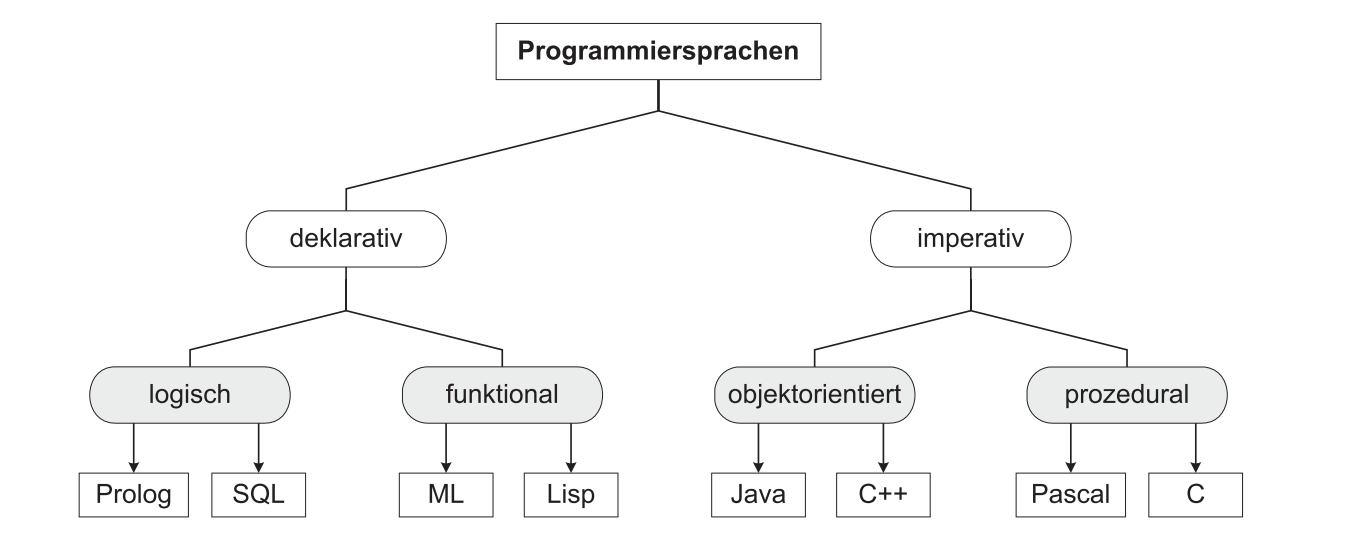
\includegraphics[width=\linewidth,height=0.5\textheight,keepaspectratio]{chapters/04_programming_languages/figures/paradigms/paradigms.png}
                    \caption{Gliederung der Programmiersprachen nach unterschiedlichen Paradigmen \cite{Muller2015}}
                \end{figure}   
            \end{frame}
            
            \begin{frame}{Programmierparadigmen: Imperativ (I)}
                \begin{figure}
                    \centering
                    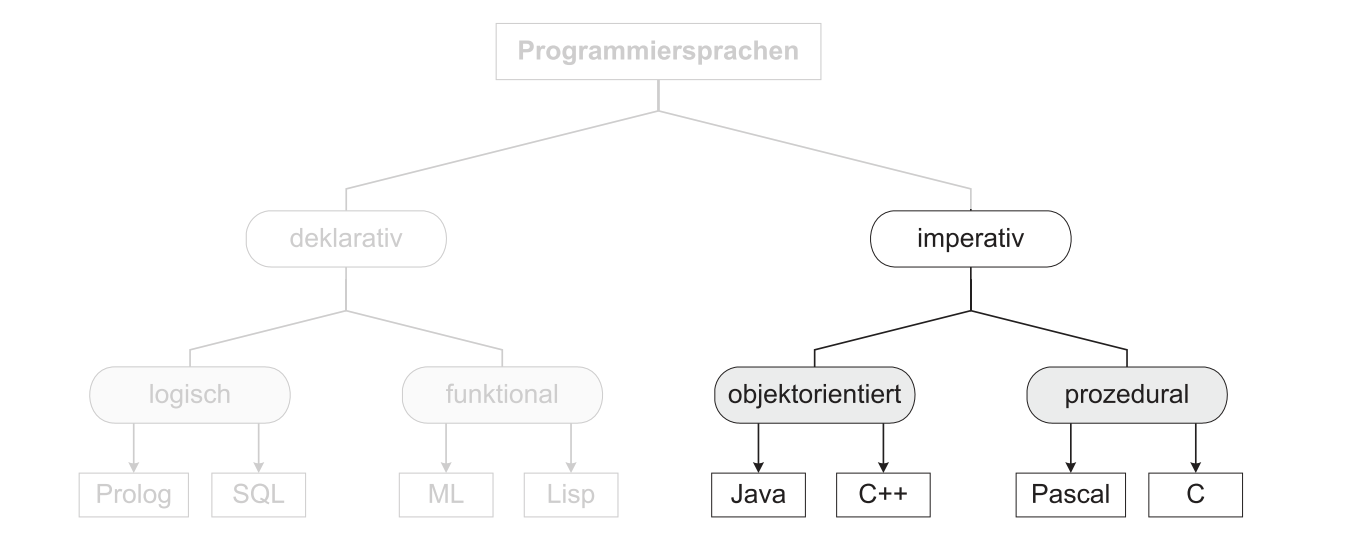
\includegraphics[width=\linewidth,height=0.5\textheight,keepaspectratio]{chapters/04_programming_languages/figures/paradigms/imperative.png}
                    \caption{Gliederung der Programmiersprachen nach unterschiedlichen Paradigmen \cite{Muller2015} (bearbeitet)}
                \end{figure}   
            \end{frame}
            
            \begin{frame}{Programmierparadigmen: Imperativ (II)}
                Bei der \textit{imperativen Programmierung} beschreibt der Programmierer, was der Reihe nach ausgeführt werden soll. Er ist also sowohl für die zugrundeliegende Funktionalität als auch für die ordnungsgemäße Reihenfolge dieser Anweisungen zuständig. \\~\
                
                Die imperative Programmierung stellt das älteste und weitverbreitetste Paradigma dar, da es große Ähnlichkeiten zum menschl. Denkprozess aufweist.\\~\
                
                \begin{block}{Imperative Programmierung}
                    Ursprung: \textit{imperare} (lat.): \textit{'anordnen', 'befehlen'} \\
                    Der Programmierer beschreibt, \textbf{wie} eine Lösung zu einem bestimmten Problem ermittelt wird.
               \end{block}
               
               \note{
                   was wird der Reihe nach ausgeführt \\
                   konkrete Befehle an den Computer, Step by Step\\
                   Programmierer ist für zugrundeliegende Funktionalität als auch für Reihenfolge der Anweisungen zuständig \\
                   einfach zu verstehen
                }
            \end{frame}
            
            \begin{frame}{Programmierparadigmen: Imperativ (III)}
                Häufig wird innerhalb der imperativen Programmierung zwischen zwei weiteren (konträren) Paradigmen unterschieden: \\~\ 
                
                \begin{columns}[T]
                    \begin{column}{0.5\textwidth}
                        \textbf{Prozedural}
                        \begin{itemize}
                            \item Programmablauf kann in Teilprobleme zerlegt werden
                            \item Wichtig zur Übersichtlichkeit, Wartbarkeit und Vermeidung von Redundanz
                            \item Daten und Funktionen haben keinen definierten Zusammenhalt
                        \end{itemize}
                    \end{column}
                    
                    \begin{column}{0.5\textwidth}
                        \textbf{Objektorientiert}      
                        \begin{itemize}
                            \item Funktionalitäten werden innerhalb von Klassen nach Zuständigkeit getrennt
                            \item Über einfache Datenstrukturen hinausgehende Abstraktion der Daten und Funktionalität 
                            \item Daten und Funktionen werden in Klassen / Objekten zusammengefasst
                        \end{itemize}
                    \end{column}
                \end{columns}
                
                \note{
                   Unterscheidung zwischen Prozedural und Objektorientiert
                }
            \end{frame}
            
            \begin{frame}{Programmierparadigmen: Deklarativ (I)}
                \begin{figure}
                    \centering
                    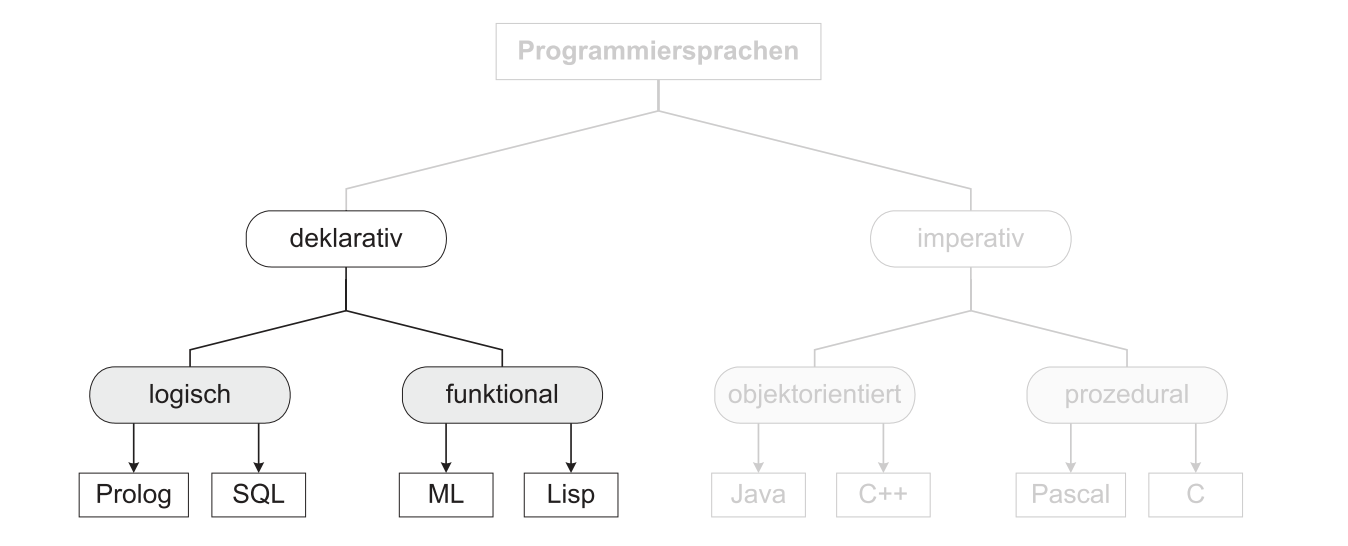
\includegraphics[width=\linewidth,height=0.5\textheight,keepaspectratio]{chapters/04_programming_languages/figures/paradigms/declarative.png}
                    \caption{Gliederung der Programmiersprachen nach unterschiedlichen Paradigmen \cite{Muller2015} (bearbeitet)}
                \end{figure}   
            \end{frame}
            
            \begin{frame}{Programmierparadigmen: Deklarativ (II)}
                Bei der \textit{deklarativen Programmierung} beschreibt der Programmierer nicht, was der Reihe nach ausgeführt werden soll, sondern \textit{was} berechnet werden soll. Dadurch steht hier vielmehr die Beschreibung des Problems als die explizite Beschreibung des Lösungswegs im Vordergrund. \\~\
                
                Im Gegensatz zur imperativen Programmierung lassen sich hier Arbeits- und Steuermechanismen trennen, sodass dieses Paradigma rechnerunabhängig ist. \\~\
                
                \begin{block}{Deklarative Programmierung}
                    Ursprung: \textit{declarar} (lat.): \textit{'erklären'} \\
                    Der Programmierer beschreibt, \textbf{was} berechnet werden soll und nicht, wie der entsprechende Rechenweg dafür aussieht.
               \end{block}
               
               \note{
                   Grundsätzlich anders als imperative Programmierung \\ 
                   Beschreibung \textbf{was} berechnet werden soll, nicht wie \\ 
                   Beschreibung des Problems ist wichtig, nicht der Lösungsweg \\
                   Trennung von Arbeits- und Steuermechanismen
                }
            \end{frame}
            
            \begin{frame}{Programmierparadigmen: Imperativ vs. Deklarativ}
            
                Beispiel: Durchsuche Bibliothekskatalog nach Büchern mit dem Titel "Programmierung" \footnote{angelehnt an \cite{leimeister}}
                
                \begin{exampleblock}{Beispiel: Imperative Programmierung}
                    \begin{enumerate}
                        \item Nimm Buch
                        \item Prüfe, ob Titel = "Programmierung"
                        \item Falls JA, notiere Autor
                        \item Prüfe, ob letztes Buch
                        \item Falls NEIN, gehe zu (1)
                        \item Falls JA \textrightarrow Ende
                    \end{enumerate}
                \end{exampleblock}
                
                \begin{exampleblock}{Beispiel: Deklarative Programmierung}
                    \begin{enumerate}
                        \item Suche alle Bücher, für die gilt (Titel = "Programmierung")
                    \end{enumerate}
                \end{exampleblock}
            \end{frame}
        
        \subsection{Maschinennähe}
            \begin{frame}{Maschinennähe}
                Beschreibt den Abstraktionsgrad bzw. die Nähe der Programmiersprache zum darunterliegenden System \\~\
                
                Maschinennahe Sprachen ("Low-Level Sprachen") bieten mehr Kontrolle und können tiefer in Systemfunktionalitäten eingreifen, sind aber meist auch komplexer und schwerer zu beherrschen als höhere Sprachen ("High-Level Sprachen") \\~\
                
                \begin{columns}[T]
                    \begin{column}{0.5\textwidth}
                        \textbf{Low-Level Sprachen}
                        
                        \begin{itemize}
                            \item Geringer oder kein Abstraktionsgrad
                            \item Direkte Speicherzugriffe, Kernelzugriffe, ... möglich
                            \item Mehr Kontrolle, höhere Komplexität
                            \item Beispiele: Maschinencode, Algol, Assembler, C
                        \end{itemize}
                    \end{column}
                    \begin{column}{0.5\textwidth}
                        \textbf{High-Level Sprachen}
                        
                        \begin{itemize}
                            \item Hoher Abstraktionsgrad
                            \item Keine direkten Speicherzugriffe, Kernelzugriffe, ... möglich
                            \item Weniger Kontrolle, geringere Komplexität
                            \item Beispiele: Java, Python, C++
                        \end{itemize}
                    \end{column}
                \end{columns}
                
                \note{
                   Grad der Abstraktion \\
                   Mehr Kontrolle, tiefe Systemeingriffe vs. Bedienungsfreundlichkeit, flache Lernkurve
                }
            \end{frame}
        
        \subsection{Computersprachen}
            \begin{frame}{Computersprachen}
                Nicht alle Sprachen, die häufig als "Programmiersprachen" bezeichnet werden, sind auch tatsächlich Programmiersprachen, da sie beispielsweise nicht alle Eigenschaften einer Programmiersprache erfüllen (siehe Abs. \ref{sec:properties}). Daher können Sprachen auch entsprechend ihres Zwecks untergliedert werden:
                
                \begin{itemize}
                    \item \textbf{Programmiersprache}: Kann komplexe Programmabläufe darstellen, besitzt alle beschriebenen Eigenschaften einer Programmiersprache (Beispiel: Python, Java, C)
                    \item \textbf{Datenbanksprache}: Wird zur Kommunikation mit einem Datenbanksystem verwendet (Beispiel: SQL)
                    \item \textbf{Auszeichnungssprache}: Beschreibt den Aufbau und die Struktur von Dokumenten (Beispiel: HTML, XML)
                    \item \textbf{Stylesheet-Sprache}: Beschreibt das Erscheinungsbild von Dokumenten unabhängig vom Inhalt (Beispiel: CSS)
                \end{itemize}
                
            
            \end{frame}

        \subsection{Typisierung}
            \begin{frame}{Typisierung / Typsysteme}
                In jeder Programmiersprache können Variablen erzeugt werden, denen unterschiedliche Arten von Werten (\textbf{Datentypen}) zugewiesen werden können. Dazu zählen bspw. Zahlen (Ganzzahlen, Fließkommazahlen), Zeichenketten (Strings) und Wahrheitswerte. Die Typisierung einer Programmiersprache dient zur korrekten Verwendung dieser Datentypen. \\~\
                
                Der Umgang mit den Datentypen kann sich zwischen den Programmiersprachen unterscheiden.
                
                \note{
                   Variablen können versch. Werte beinhalten \\
                   Ganzzahlen , Fließkommazahlen, Strings, Warhheitswerte \\
                   korrekte Verwendung der Datentypen
                }
            \end{frame}
            
            \begin{frame}{Typisierung / Typsysteme: Typenlose Sprachen}
                Manche Sprachen sind typenlose Sprachen. Derartige Programmiersprachen verfügen über keine differenzierten Datentypen. Das ist für den Entwickler einerseits sehr bequem, da er sich nicht um die entsprechenden Datentypen kümmern muss, führt aber auch schnell zu Fehlern, die aufgrund fehlender Typbezeichnungen manchmal nur schwer festzustellen und zu finden sind.  \\~\
                
                Beispiel: Assembler
                
                \note{
                   Verfügen über keine differenzierten Datentypen \\
                   bequem aber fehleranfällig
                }
                
            \end{frame}
            
            \begin{frame}{Typisierung / Typsysteme: Typisierte Sprachen}
                Die meisten Programmiersprachen sind typisiert, d.h. alle Variablen besitzen jederzeit einen bestimmten Datentyp. \\~\
                
                Typsysteme können weiter klassifiziert werden:
                \begin{itemize}
                    \item Statische vs. dynamische Typisierung: Typprüfungen finden zur Übersetzungszeit (statisch) oder zur Laufzeit (dynamisch) statt
                    \item Explizite vs. implizite Typisierung: Datentypen werden explizit genannt oder implizit ermittelt
                    \item Starke vs. schwache Typisierung: Verlustbehaftete Typumwandlungen können nicht (stark) / können (schwach) durchgeführt werden
                \end{itemize}
                
                \note{
                   alle Variablen besitzen einen Datentyp \\
                   statisch / dynamisch: Prüfung zur Runtime vs Compiletime \\
                   explizit / implizit \\
                   stark vs. schwach: Verlustbehaftete Umwandlung möglich
                   
                   
                }
            \end{frame}
            
            \begin{frame}{Anwendungsbereich}
                Manche Programmiersprachen werden nur domänenspezifisch eingesetzt, andere sind universell einsetzbar \footnote{Fettgedruckte Sprachen sind explizit für den jeweiligen Einsatzbereich entwickelt und werden ausschließlich dort verwendet}.
                
                \begin{itemize}
                    \item Websprachen (Serverseitig): \textbf{PHP}, \textbf{Ruby}, \textbf{node.js}, Python, Java
                    \item Websprachen (Clientseitig): \textbf{JavaScript}
                    \item Mobile Applications: \textbf{Kotlin} / Java (Android), \textbf{Swift} / Objective-C (iOS)
                    \item Business Applications: Java, C++, C\#
                    \item Datenbanken: \textbf{SQL}
                \end{itemize}
            \end{frame}
            
            
            \subsection{Appendix}
            
            \begin{frame}{Antwort 1: Was hat das mit Programmiersprachen zu tun?}

                \begin{columns}
                    \begin{column}{0.4\linewidth}
                        \begin{figure}
                            \centering
                            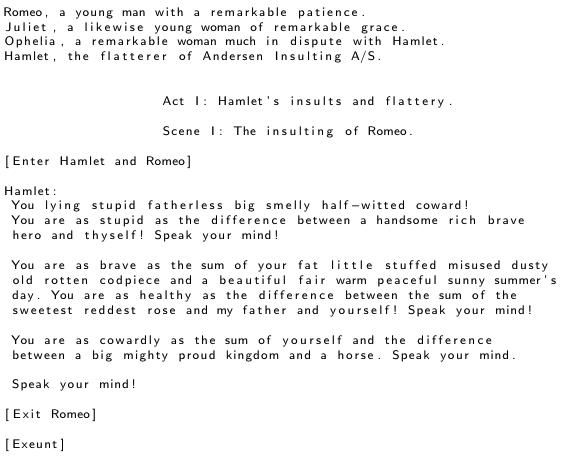
\includegraphics[width=\linewidth,height=0.5\textheight,keepaspectratio]{chapters/04_programming_languages/figures/shakespeare_code.png}
                        \end{figure}
                    \end{column}
                    \begin{column}{0.6\linewidth}
                        \begin{figure}
                            \centering
                            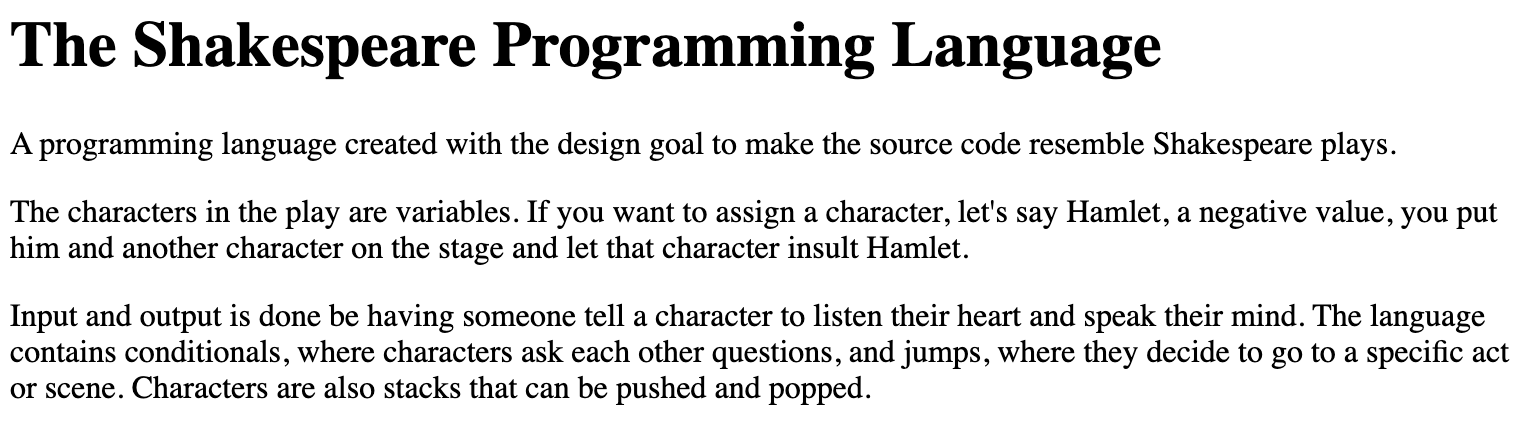
\includegraphics[width=\linewidth,height=0.5\textheight,keepaspectratio]{chapters/04_programming_languages/figures/shakespeare.png}
                            \caption{The Shakespeare Programming Language \cite{shakespeare_pl}}
                        \end{figure}
                    \end{column}
                \end{columns}
                \note{
                Titel: frei gewählt, keine Bedeutung \\
                Charaktere: Zu Beginn müssen die Personen festgelegt werden (Variablen) \\
                Akte \& Szenen: Sprungmarken, ansonsten nicht berücksichtigt \\
                Enter, Exit \& Exeunt: Charaktere müssen auf der Bühne stehen \\
                Dialog: Anweisungen, Eingabe, Ausgabe, Kontrollanweisungen \\
                Literale: negative Konnotation (-1), neutral (0), positive Konnotation (+1)
                }
                
            \end{frame}
            
             \begin{frame}{Antwort 2: Was hat das mit Programmiersprachen zu tun?}
                \begin{columns}
                    \begin{column}{0.4\linewidth}
                        \begin{figure}
                            \centering
                            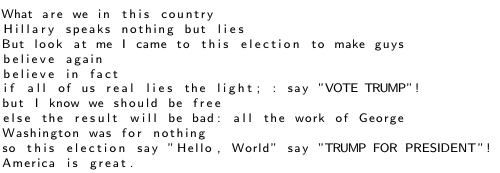
\includegraphics[width=\linewidth,height=0.5\textheight,keepaspectratio]{chapters/04_programming_languages/figures/trump_code.png}
                        \end{figure}
                    \end{column}
                    \begin{column}{0.6\linewidth}
                        \begin{figure}
                            \centering
                            
\includegraphics[width=\linewidth,height=0.5\textheight,keepaspectratio]{chapters/04_programming_languages/figures/trump.png}
                            \caption{TrumpScript \cite{trumpscript}}
                        \end{figure}
                    \end{column}
                \end{columns}
                
                \note{\href{https://github.com/samshadwell/TrumpScript}{https://github.com/samshadwell/TrumpScript}}
            \end{frame}
            
            \begin{frame}{Antwort 3: Was hat das mit Programmiersprachen zu tun?}
                \begin{columns}
                    \begin{column}{0.4\linewidth}
                       \begin{figure}
                    \centering
                    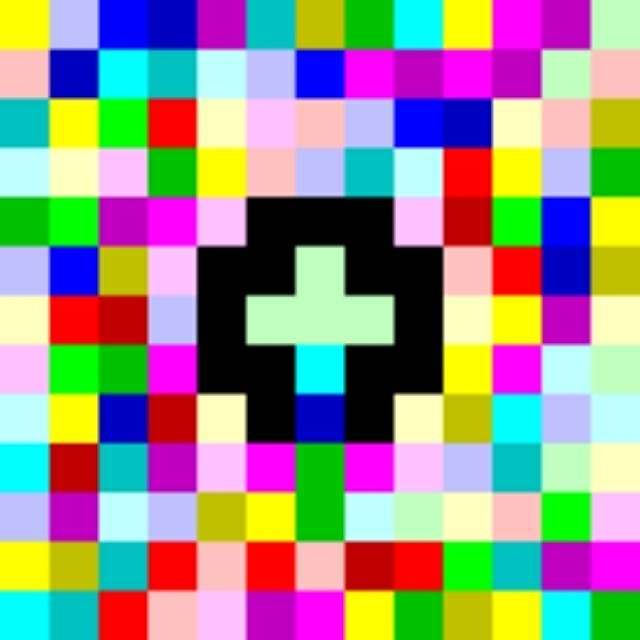
\includegraphics[width=\linewidth,height=0.5\textheight,keepaspectratio]{chapters/04_programming_languages/figures/hello_world_piet.jpg}
                    \caption{\cite{fig:hello_world_piet}}
                \end{figure}
                    \end{column}
                    \begin{column}{0.6\linewidth}
                        \begin{figure}
                            \centering
                            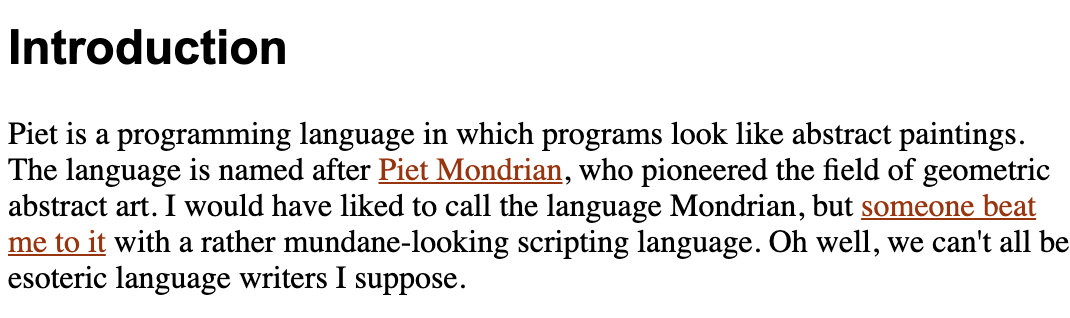
\includegraphics[width=\linewidth,height=0.5\textheight,keepaspectratio]{chapters/04_programming_languages/figures/piet.png}
                            \caption{Piet \cite{piet}}
                        \end{figure}
                    \end{column}
                \end{columns}
                
                \note{
                Code sieht wie ein abstraktes Bild aus \\
                kleinste Einheit: Codel (Code + Pixel) \\
                Werte: Eintreten in schwarzes oder weißes Farbfeld, Zahl der Codels mit zusammenhängender Farbe oder Übergang von einer Farbe zur nächsten
                }
            \end{frame}
        
            
            \begin{frame}{Antwort 4: Was hat das mit Programmiersprachen zu tun?}
                 \lstinputlisting[basicstyle=\tiny]{chapters/04_programming_languages/code/hello_world.bf}
                 
                 \begin{figure}
                            \centering
                            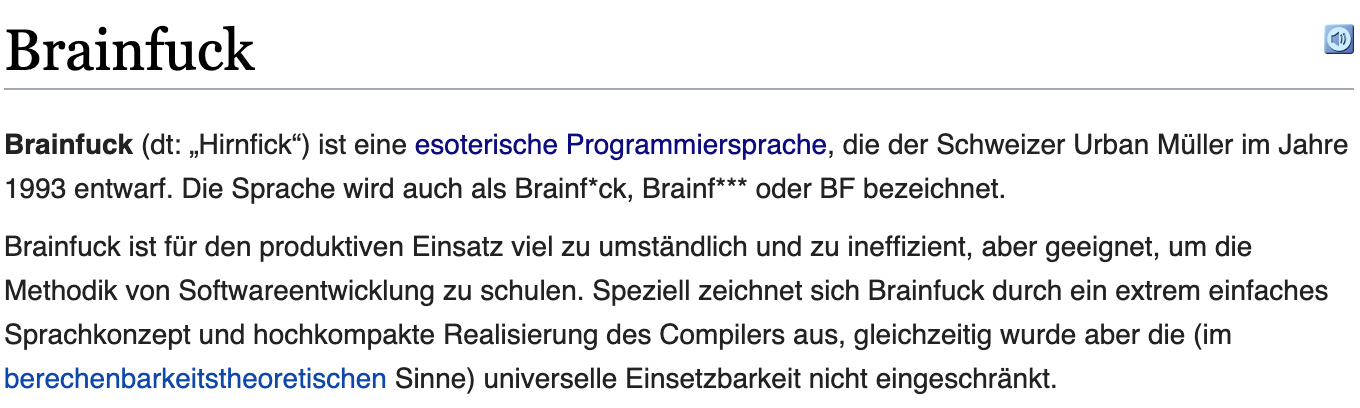
\includegraphics[width=0.7\linewidth,height=0.5\textheight,keepaspectratio]{chapters/04_programming_languages/figures/brainfuck.png}
                            \caption{Brainfuck \cite{brainfuck}}
                \end{figure}
                        
                \note{
                    Jedes Zeichen hat eine unterschiedliche Bedeutung: \\
                    $>$ inkrementiert den Zeiger \\
                    + inkrementiert den aktuellen Zellenwert \\
                    . gibt das aktuelle Zeichen aus
                }
            \end{frame}
%\newcommand{\decktitle}{Kommandozeile}

%%%%%%%%%%%%%%%%%%%%%%%%%%%%%%%%%%%%%%%%%%%%%%%%%
%
% DOCUMENT
%
%%%%%%%%%%%%%%%%%%%%%%%%%%%%%%%%%%%%%%%%%%%%%%%%%

\begin{frame}
    \subtitle{\decktitle}
    \titlepage
\end{frame}


\begin{frame}
    \frametitle{\textbf{Outline:}}
    \tableofcontents
\end{frame}

		
		   
\section{Kommandozeile}

    \begin{frame}{Was ist die Kommandozeile?}
    
        \begin{itemize}
            \item Annähernd jedes Betriebssystem besitzt eine Kommandozeile
            \item Eine Kommandozeile nimmt Befehle vom Nutzer, die dieser bspw. eintippen kann, entgegen und führt diese aus
            \item Zu Beginn des Computerzeitalters war dies oftmals die einzige Möglichkeit, Befehle / Programme auszuführen, da graphische Benutzeroberflächen (GUIs) erst später verbreitet waren
            \item Auch heute wird die Kommandozeile noch häufig verwendet (insbesondere von Entwicklern), da hierdurch Befehle sehr schnell ausgeführt werden können und der Nutzer nicht erst in der GUI danach suchen muss
            \item Die Kommandozeile besitzt verschiedene Namen: \textit{Eingabeaufforderung}, \textit{Befehlszeile}, \textit{Terminal}, \textit{CLI (command-line interface)}, \textit{command prompt}, ...
        \end{itemize}
    \end{frame}
    
    \begin{frame}{Wofür benötigen wir die Kommandozeile?}
        In der Programmierung ist die Kommandozeile unabdingbar. Oftmals sind Befehle notwendig, die über die GUI nur sehr schwer (oder überhaupt nicht) ausgeführt werden können, außerdem trägt die Verwendung der Kommandozeile zum Grundverständnis verschiedenster Operationen bei. \\~\
        
        Eine Auswahl der wichtigsten Operationen werden im Folgenden vorgestellt und sollen im Anschluss auch angewendet werden können.
    \end{frame}
    
    
    \begin{frame}{Öffnen der Kommandozeile (Windows 10)}
        In Windows wird die Kommandozeile im Deutschen "\textit{Eingabeaufforderung}" genannt. Diese kann auf unterschiedliche Arten geöffnet werden:
        
        \begin{itemize}
            \item Start \textrightarrow Windows-System \textrightarrow Eingabeaufforderung
            \item \texttt{WIN}-Taste + \texttt{R} \textrightarrow  \texttt{cmd} eingeben \textrightarrow Bestätigen
        \end{itemize}
        
        
        \begin{figure}
            \centering
            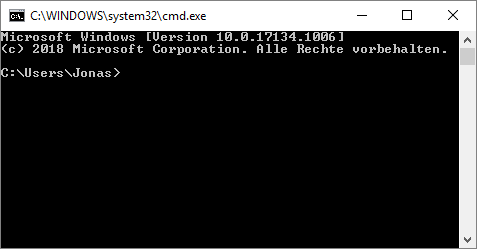
\includegraphics[width=0.8\linewidth,height=0.5\textheight,keepaspectratio]{chapters/05_command_line/figures/cmd_win.png}
            \caption{Die Windows-Eingabeaufforderung}
        \end{figure}
        
    \end{frame}
    
    \begin{frame}{Öffnen der Kommandozeile (macOS)}
        In macOS wird die Kommandozeile "\textit{Terminal}" genannt. Diese kann folgendermaßen geöffnet werden:
        
        \begin{itemize}
            \item Finder \textrightarrow Programme \textrightarrow Dienstprogramme \textrightarrow Terminal
        \end{itemize}
        
        \begin{figure}
            \centering
            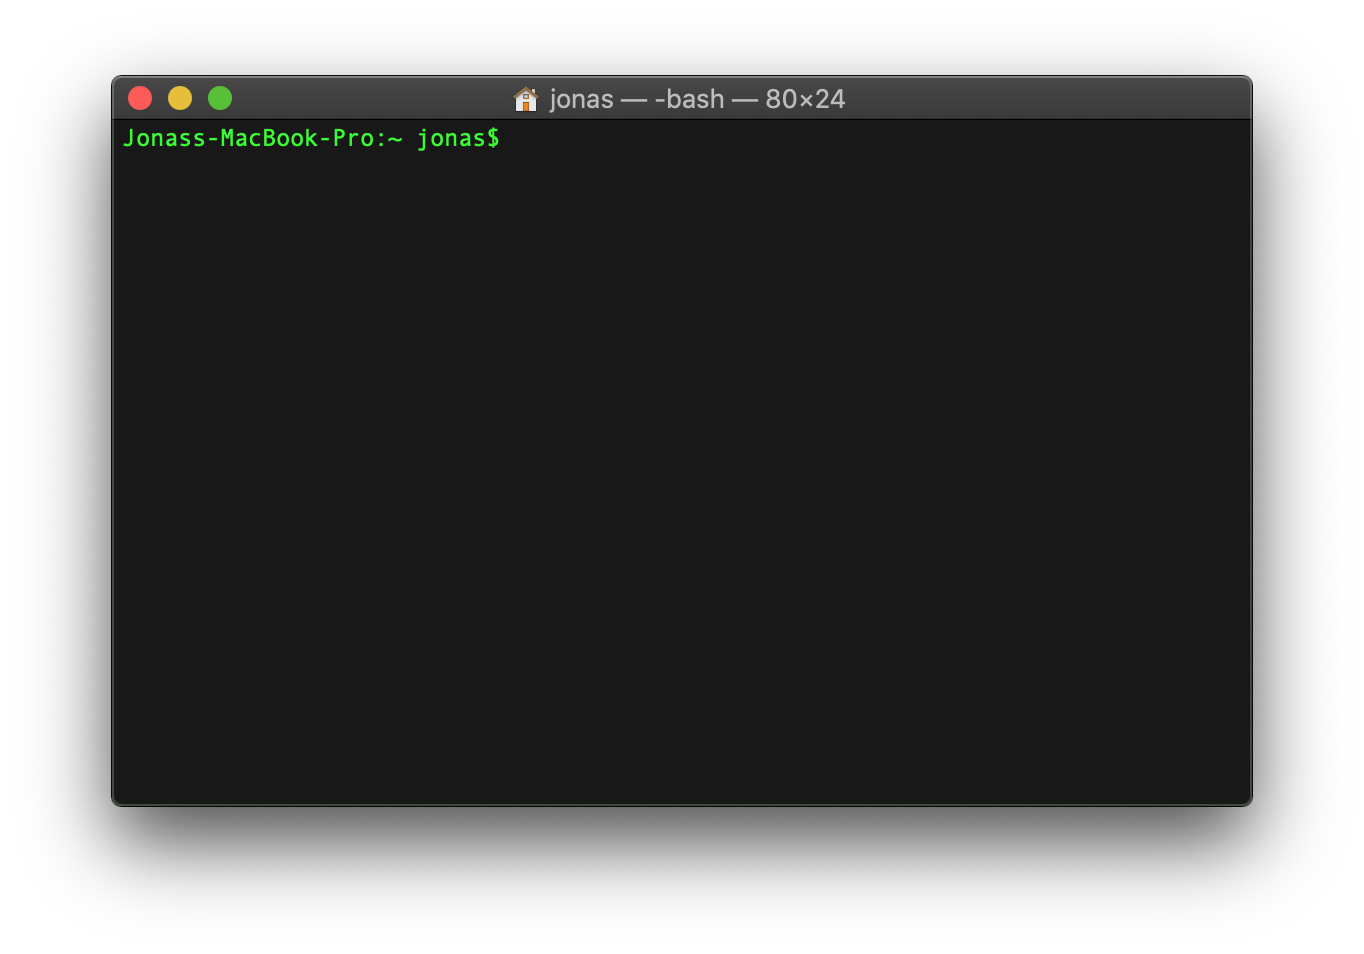
\includegraphics[width=0.8\linewidth,height=0.5\textheight,keepaspectratio]{chapters/05_command_line/figures/cmd_mac.png}
            \caption{Die macOS-Eingabeaufforderung}
        \end{figure}
    \end{frame}

    \begin{frame}{Verwenden der Kommandozeile}
        Mithilfe der Kommandozeile ist es möglich, ebenso wie mit dem Windows Dateiexplorer bzw. dem Finder auf macOS, durch das Dateisystem zu navigieren.
        Die Kommandozeile zeigt stets an, in welchem Ordner sich der Nutzer aktuell befindet. \\~\
        
        Wird also angezeigt \code{C:\textbackslash{}Users\textbackslash{}Jonas} bedeutet das, dass sich der Nutzer aktuell in seinem Nutzerverzeichnis befindet. Bei macOS enthält die Anzeige (z.B. \code{Jonas-MacBook-Pro:$\sim$ jonas}) standardmäßig noch zusätzliche Informationen: Der erste Teil bezieht sich auf den Computernamen (\code{Jonas-MacBook-Pro}), nach dem Doppelpunkt folgt der aktuelle Ordner (\code{$\sim$}), sowie der aktuell angemeldete Nutzer (\code{jonas}).
    \end{frame}
    
    \begin{frame}{Verwenden der Kommandozeile}
        \begin{alertblock}{Achtung}
            Bei Windows werden Dateipfade standardmäßig mit Backslash (\code{\textbackslash{}}) geschrieben. Auf unixoiden Systemen wie macOS oder Linux wird standardmäßig ein Forwardslash (\code{/}) verwendet.
        \end{alertblock}
    \end{frame}
    
    \begin{frame}{Verwenden der Kommandozeile - Dateisystem}
        In der Regel sind die Dateisysteme bei allen Betriebssystemen hierarchisch aufgebaut. \\~\
        
        \begin{itemize}
            \item \textbf{Windows:} Bei Windows bekommt jede Speichereinheit (z.B. Festplatte) einen Buchstaben zugewiesen. Die primäre Speichereinheit trägt i.d.R. den Namen \code{C}. Diese Speicherinhalt beinhaltet dann verschiedene Dateien und Verzeichnisse, welche wiederum Dateien und Verzeichnisse enthalten können. Ein Unterverzeichnis von C kann z.B. der Ordner \texttt{Benutzer} (oder \texttt{Users}) sein, in dem alle benutzerspezifischen Informationen abgelegt sind. Ein weiterer Ordner ist bspw. \texttt{Programme}, der alle notwendigen Dateien der installierten Programme beinhaltet.
        \end{itemize}
    \end{frame}
    
    \begin{frame}{Verwenden der Kommandozeile - Dateisystem}
       
        \begin{itemize}
            \item \textbf{macOS:} In unixoiden Betriebssystem ist das Dateisystem ebenfalls hierarchisch, jedoch etwas anders aufgebaut. Während es bei Windows mehrere \textit{Roots} geben kann (eine für jede Speichereinheit), gibt es bei unixoiden System stets lediglich eine \textit{Root}, nämlich \code{/}. Hierunter befinden sich ebenfalls hierarchisch die verschiedenen Ordner und Dateien. In Abb. \ref{fig:file_system} wird der Aufbau der Dateisysteme exemplarisch gezeigt.
        \end{itemize}
    \end{frame}
    
     \begin{frame}{Verwenden der Kommandozeile - Dateisystem}
       
       \begin{figure}
            \centering
            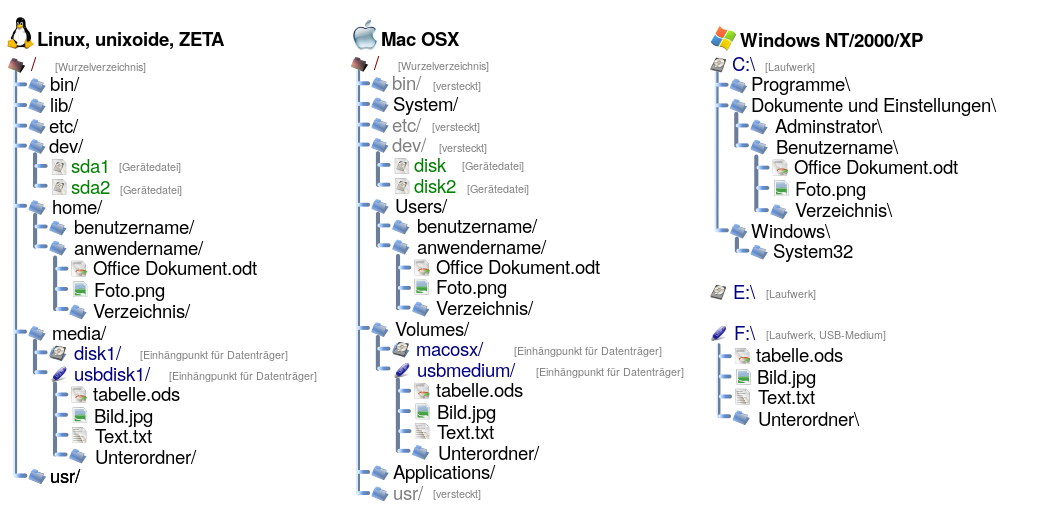
\includegraphics[width=\linewidth,height=0.7\textheight,keepaspectratio]{chapters/05_command_line/figures/Filesystem.png}
            \caption{Vergleich der Verzeichnisstruktur verschiedener Betriebssysteme \cite{filesystems}}
            \label{fig:file_system}
        \end{figure}
    \end{frame}
    
     \begin{frame}{Verwenden der Kommandozeile - Navigieren}
        Wie mit dem Dateiexplorer auch kann mithilfe der Kommandozeile durch die Verzeichnisse navigiert werden. Der Befehl hierfür lautet \code{cd} ("change directory"). \\~\
        
        Es kann entweder ein \textbf{absoluter} Pfad, der das Verzeichnis ausgehend von der Root beschreibt, oder ein \textbf{relativer} Pfad, der das Verzeichnis ausgehend vom aktuellen Verzeichnis beschreibt, angegeben werden. \\~\
        
        Bei Windows beginnt ein absoluter Pfad immer mit \code{C:\textbackslash{}} bzw. \code{\textbackslash{}}. Bei macOS beginnt ein absoluter Pfad immer mit \code{/}.
     \end{frame}
     
     
     \begin{frame}{Verwenden der Kommandozeile - Navigieren}
        
        \begin{itemize}
            \item \textbf{Betreten eines nächst-tieferen Verzeichnisses:} Angenommen das Verzeichnis, in dem sich der Nutzer gerade befindet, beinhaltet ein Verzeichnis mit dem Namen \textit{Programming}. Nun kann in dieses Verzeichnis gewechselt werden, in dem der Nutzer folgenden Befehl eingibt: \\~\
            
            \code{cd Programming}
            
            Dies stellt einen relativen Pfad dar, da ausgehend vom aktuellen Verzeichnis in das "tiefere" Verzeichnis "Programming" gewechselt wird. Folgende absolute Pfadangabe wäre äquivalent: \\~\
            
            \code{cd C:\textbackslash{}Users\textbackslash{}Jonas\textbackslash{}Programming} (Windows) bzw. \code{cd /Users/Jonas/Programming} (macOS)
            
        \end{itemize}
        
     
     \end{frame}
     
      \begin{frame}{Verwenden der Kommandozeile - Navigieren}
        
        \begin{itemize}
         
            \item \textbf{Betreten des übergeordneten Verzeichnisses:} Der Nutzer kann in das übergeordnete Verzeichnis wechseln, indem er folgendes eingibt: \\~\
            
            \code{cd ..}
            
            \begin{block}{Hinweis}
                \code{..} steht üblicherweise als Abkürzung für das übergeordnete Verzeichnis, während \code{.} für das aktuelle Verzeichnis steht
            \end{block}
        \end{itemize}
    
     \end{frame}
     
      \begin{frame}{Verwenden der Kommandozeile - Navigieren}
        
        \begin{itemize}
         
            \item \textbf{Betreten des Nutzerverzeichnisses:}
                
                \begin{itemize}
                    \item \textbf{macOS:} Unter macOS gibt es eine Kurzschreibweise um in das Nutzerverzeichnis (Home-Verzeichnis) zu wechseln. Auf unixoiden System steht das Symbol \code{$\sim$} i.d.R. für das Nutzerverzeichnis, also reicht der folgende Befehl aus: \\~\
                
                    \code{cd $\sim$} bzw. \code{cd} (äquivalent zu \code{cd /Users/Jonas/}) \\~\
                    
                    \item \textbf{Windows:} Bei Windows existiert eine solche Kurzform nicht, falls aber die Umgebungsvariable \code{HOMEPATH} gesetzt ist, kann dieser Befehl genutzt werden: \\~\
                
                \code{cd \%HOMEPATH\%}
                \end{itemize}
                
        \end{itemize}
    \end{frame}
    
    \begin{frame}{Verwenden der Kommandozeile - Anzeigen des aktuellen Verzeichnisses}
        Um den kompletten (absoluten) Pfad des Verzeichnisses, in dem sich der Nutzer derzeit befindet, anzuzeigen, gibt es betriebssystemspezifische Befehle:
        
        \begin{itemize}
            \item \textbf{Windows:} \code{cd}
            \item \textbf{macOS:} \code{pwd} (print working directory)
        \end{itemize}
    \end{frame}
    
    \begin{frame}{Verwenden der Kommandozeile - Anzeigen von Verzeichnisinhalten}
        Um die Inhalte von Verzeichnissen anzuzeigen, also alle im derzeitigen Verzeichnis enthaltenen Dateien und Ordner, gibt es für Windows und macOS verschiedene Befehle:
        
        \begin{itemize}
            \item \textbf{Windows:} \code{dir} (directory)
            \item \textbf{macOS:} \code{ls} (list) (bzw. \code{ls -l}, um die Inhalte in einer Liste mit Details anzuzeigen)
        \end{itemize}
    \end{frame}
    
    
     \begin{frame}{Verwenden der Kommandozeile - Anlegen von Verzeichnissen}
        
        Mithilfe der Kommandozeile können auch Verzeichnisse angelegt werden, ebenso wie im Datei-Explorer ein neuer Ordner angelegt werden kann.\\~\
        
        Hierfür existiert der \code{mkdir}-Befehl. Dieser Benötigt jedoch noch ein zusätzliches \textit{Argument}, mit dem der Name des Verzeichnisses mit angegeben werden kann, also z.B. \\~\
        
        \code{mkdir Programming} \\~\
        
        Hierdurch wird im aktuellen Verzeichnis ein Ordner mit dem Namen "Programming" erzeugt.
    \end{frame}
    
    \begin{frame}{Verwenden der Kommandozeile - Löschen von Verzeichnissen}
        
        Auch ein Löschen von Verzeichnissen und Dateien ist möglich.\\~\
        
        \begin{alertblock}{Achtung}
            Durch das Löschen von Verzeichnissen und Dateien können Informationen unwiderruflich verloren gehen. Es muss also sichergestellt werden, dass lediglich Elemente gelöscht werden, die gelöscht werden sollen.
        \end{alertblock}
        
        \begin{itemize}
            \item \textbf{Windows:} 
                \begin{itemize}
                    \item \textbf{Löschen einer Datei:} \code{del <Dateiname>}
                    \item \textbf{Löschen eines Verzeichnisses:} \code{rmdir /S /Q <Verzeichnisname>}
                \end{itemize}
            \item \textbf{macOS:}
                \begin{itemize}
                    \item \textbf{Löschen einer Datei:} \code{rm <Dateiname>}
                    \item \textbf{Löschen eines Verzeichnisses:} \code{rm -rf <Verzeichnisname>}
                \end{itemize}
        \end{itemize}
        
    \end{frame}
    
    
    \begin{frame}{Verwenden der Kommandozeile - Kopieren von Dateien}
        
        Mithilfe der Kommandozeile können Dateien ebenso wie über den Explorer in andere Verzeichnisse kopiert werden. \\~\
        
        Hierfür existiert der \code{copy} (Windows) bzw. \code{cp} (macOS) Befehl. Dieser Befehl besitzt zwei Argumente: Als erstes muss die Datei angegeben werden, die kopiert werden soll, als zweites muss der Zielpfad spezifiziert werden, z.B.: \\~\
        
        \code{copy main.py ..\textbackslash{}} bzw. \code{cp main.py ../}\\~\
        
        Mithilfe dieses Befehls wird die Datei \code{main.py} aus dem aktuellen Verzeichnis in das übergeordnete Verzeichnis (\code{../}) kopiert.
        
    \end{frame}
    
    \begin{frame}{Verwenden der Kommandozeile - Verschieben von Dateien}
        
        Mithilfe der Kommandozeile können Dateien ebenso wie über den Explorer in andere Verzeichnisse verschoben werden. \\~\
        
        Hierfür existiert der \code{move} (Windows) bzw. \code{mv} (macOS) Befehl. Dieser Befehl besitzt zwei Argumente: Als erstes muss die Datei angegeben werden, die verschoben werden soll, als zweites muss der Zielpfad spezifiziert werden, z.B.: \\~\
        
        \code{move main.py ..\textbackslash{}} bzw. \code{mv main.py ../}\\~\
        
        Mithilfe dieses Befehls wird die Datei \code{main.py} aus dem aktuellen Verzeichnis in das übergeordnete Verzeichnis (\code{../}) verschoben.
        
    \end{frame}
    
\begin{frame}{Verwenden der Kommandozeile - Tipps}
    
    \begin{block}{Ergänzung von Befehlen}
      Mithilfe der Tabulator-Taste können gewisse Befehle und Dateinamen ergänzt werden, wenn die Anfangsbuchstaben eingegeben wurden. \\~\
      
      Beispiel: Es existiert eine Datei namens \code{main.py} im aktuellen Verzeichnis. Wird nun \code{copy ma} eingegeben und anschließend die Tabulator-Taste gedrückt, wird der Dateiname automatisch ergänzt.
    \end{block}
    
    \begin{block}{Durchsuchen des Befehlsverlaufs}
      Mithilfe der Pfeil-Tasten (\textuparrow / \textdownarrow) können die letzten Befehle durchgegangen und erneut ausgeführt werden.
      
    \end{block}
\end{frame}
    
\begin{frame}{Verwenden der Kommandozeile - Befehlsübersicht}
    
    Die unterschiedlichen Befehle, die innerhalb der Kommandozeile angewendet werden können, sind u.a. in folgenden Übersichten zum Nachschlagen zusammengefasst:
    
\begin{itemize}
    \item \href{http://www.cs.columbia.edu/~sedwards/classes/2017/1102-spring/Command\%20Prompt\%20Cheatsheet.pdf}{Windows-Cheatsheet}
    
    \item \href{https://www2.icp.uni-stuttgart.de/~icp/mediawiki/images/b/bd/Sim_Meth_I_T0_cheat_sheet_10_11.pdf}{Unix-Cheatsheet}
\end{itemize}
\end{frame}
    
    \begin{subsection}{Aufgaben}
        
        \begin{frame}[allowframebreaks]{Aufgaben}
            \begin{enumerate}
            
                \item Worin besteht der primäre Unterschied zwischen dem Windows- und den unixoiden Dateisystemen?
                \item Worin unterscheiden sich absolute und relative Dateipfade?
                \item Wofür steht \code{.} und \code{..}?
                \item Wechseln Sie in ihr Home-Verzeichnis, legen Sie einen Ordner namens "Projects" sowie einen darin enthaltenes Verzeichnis "Python" und erstellen Sie darin eine Datei namens "main.py". Welche Befehle sind hierfür notwendig?
                
                \item Löschen Sie den zuvor angelegten Ordner "Projects". Was muss dabei berücksichtigt werden? Wofür stehen die Zeichen vor dem Verzeichnisnamen und wofür werden sie benötigt?
                
                \framebreak
                
                \item Ausgehend vom Pfad \code{C:\textbackslash{}Users\textbackslash{}Jonas} bzw \code{/Users/Jonas} werden folgende Befehle ausgeführt:
                
                \code{mkdir Projects}
                
                \code{mkdir Projects/Programming}
                
                \code{cd Projects}
                
                \code{pwd}
                
                Welche Ausgabe erfolgt?
                
                \item Wechseln Sie in ihr Download-Verzeichnis, erstellen Sie dort eine Datei namens \code{test.py} und benennen Sie diese in \code{main.py} um
            \end{enumerate}
        \end{frame}    
    
    \end{subsection}
%\newcommand{\decktitle}{Python I - Allgemeines}

%%%%%%%%%%%%%%%%%%%%%%%%%%%%%%%%%%%%%%%%%%%%%%%%%
%
% DOCUMENT
%
%%%%%%%%%%%%%%%%%%%%%%%%%%%%%%%%%%%%%%%%%%%%%%%%%

\begin{frame}
    \subtitle{\decktitle}
    \titlepage
\end{frame}


\begin{frame}
    \frametitle{\textbf{Outline:}}
    \tableofcontents
\end{frame}

		
		
\section{Über Python}

    \begin{frame}{Python Historie}
        \begin{itemize}
            \item Entwickelt in den 1990er Jahren vom Niederländer \textbf{Guido van Rossum} im Rahmen seiner Tätigkeit am Centrum Wiskunde \& Informatica in Amsterdam
            \item Python Version 1.0 ist im Januar 1994 erschienen
            \item Python Version 2.0 ist im Oktober 2000 erschienen
            \item Python Version 3.0 ist im Dezember 2008 erschienen
            \item Nachdem lange Zeit sowohl Python 2 als auch Python 3 unterstützt wurden, wird der offizielle Support von Python 2 zum 31.12.2019 eingestellt. Daher sollte ausschließlich Python 3 verwendet werden
        \end{itemize}
    \end{frame}
    
    
    \begin{frame}{Warum Python?}
        Python ist äußerst einsteigerfreundlich und intuitiv in der Anwendung
        
        \begin{exampleblock}{Beispiel}
        Ausgabe von 'Hello World' im Vergleich: C (links), Java (mitte) und Python (rechts)
        \end{exampleblock}
        
        \begin{columns}[T]
            \begin{column}{0.3\linewidth}
                \lstinputlisting[basicstyle=\tiny,language=C]{chapters/06_python1_introduction/code/hello_world.c}
            \end{column}
            
            \begin{column}{0.3\linewidth}
                \lstinputlisting[basicstyle=\tiny,language=Java]{chapters/06_python1_introduction/code/hello_world.java}
            \end{column}

            \begin{column}{0.3\linewidth}
                \lstinputlisting[basicstyle=\tiny,language=Python]{chapters/06_python1_introduction/code/hello_world.py}
            \end{column}            
        \end{columns}
    \end{frame}
    
    \begin{frame}{Python: Ziele}
        
        Ursprüngliche Ziele von Python, die 1999 von van Rossum im Essay "Computer Programming for Everybody" festgehalten wurden \cite{python_darpa}:
        
        \begin{itemize}
            \item Einfache und intuitive Sprache, die dennoch sehr umfangreich und mächtig ist
            \item Die Sprache soll Open Source (quelloffen) sein, sodass die Sprache als Gemeinschaftsprojekt weiterentwickelt werden kann
            \item Einfach zu lesender Quellcode, der dem Englischen möglichst nahe sein soll
            \item Hohe Praktikabilität, es sollen schnelle Entwicklungszeiten möglich sein
        \end{itemize}
    \end{frame}
    
    \begin{frame}{Python: Eigenschaften}
        Python...
        \begin{itemize}
            \item ist sowohl \textbf{einsteigerfreundlich}, als auch für professionelle Anwendungen und umfassende Business-Anwendungen geeignet
            \item ist eine \textbf{universelle} Programmiersprache, d.h. sie ist nicht nur domänenspezifisch einsetzbar (Häufige Anwendungsgebiete: Web (serverseitig), AI, Desktop-Anwendungen, mathematische Anwendungen, ...)
            \item ist eine \textbf{höhere} Programmiersprache
            \item ist (meist) eine \textbf{interpretierte} Programmiersprache
            \item ist eine \textbf{Multiparadigmensprache}, z.B. Objektorientiert, aspektorientiert, funktional, imperativ, prozedural, ...
            \item ist \textbf{dynamisch typisiert} 
            \item wird häufig als \textbf{Skriptsprache} genutzt
        \end{itemize}
    \end{frame}
    
    \begin{frame}{Python: Grundkonzepte}
        Festgehalten in "The Zen of Python":
        
        \begin{quote}
            Beautiful is better than ugly.\\
            Explicit is better than implicit.   \\
            Simple is better than complex.\\
            Complex is better than complicated.\\
            Flat is better than nested.\\
            Sparse is better than dense.\\
            Readability counts.\\
            Special cases aren't special enough to break the rules.\\
            Although practicality beats purity.\\
            Errors should never pass silently.\\
            Unless explicitly silenced.\\
            In the face of ambiguity, refuse the temptation to guess.\\
            There should be one-- and preferably only one --obvious way to do it.\\
            Although that way may not be obvious at first unless you're Dutch.\\
            Now is better than never.\\
            Although never is often better than *right* now.\\
            If the implementation is hard to explain, it's a bad idea.\\
            If the implementation is easy to explain, it may be a good idea.\\
            Namespaces are one honking great idea -- let's do more of those!\\
        \end{quote}
    \end{frame}
    
    \begin{frame}{Python: Besonderheiten}
        \begin{alertblock}{Einrückungen}
        Anders als bei den meisten anderen Programmiersprachen werden bei Python einzelne Codeblöcke (Scopes) nicht durch geschweifte Klammern gekennzeichnet, sondern aus Gründen der Übersichtlichkeit durch Einrückungen. Ein neuer Codeblock wird also eingerückt, ist der Block abgeschlossen erfolgt eine Ausrückung.
        \end{alertblock}
        
        \begin{alertblock}{Tabulator vs. Leerzeichen}
        Es ist dem Entwickler überlassen, ob er für Einrückungen jeweils 1 Tabulatorzeichen oder 8 Leerzeichen verwendet. Dies muss jedoch im kompletten Codetext einheitlich sein, da ansonsten ein Fehler auftritt (\code{IndentationError: expected an indented block})
        \end{alertblock}
    \end{frame}
    
 
\section{Interpreter}

    \begin{frame}[fragile]{Hinweise zur Darstellung I - Interaktiver Interpreter}
        
        Im Folgenden werden zu den jeweiligen Themen beispielhafte Codeausschnitte (Snippets) gezeigt, um eine Umsetzung in der Praxis zu erleichtern. 
        
        Folgende Darstellung wird genutzt, um eine Verwendung des Python-Codes innerhalb des interaktiven Python-Interpreters zu kennzeichnen:
\begin{pyconcode}
>>> x = 1
>>> print('Hello world')
Hello world
\end{pyconcode}
    
    Zeilen beginnend mit \code{>>>} stellen Eingaben / Befehle dar, während Zeilen ohne führende Größer-Zeichen die entsprechenden Ausgaben wiedergeben.
    \end{frame}
    
    \begin{frame}[fragile]{Hinweise zur Darstellung II - Ausführbare Snippets}
        Python-Snippets, die nicht im interaktiven Interpreter ausgeführt werden, sondern beispielsweise in einer Python-Datei enthalten sind, werden ähnlich dargestellt:
        
\begin{pythoncode}
import re

txt = 'abc, def, ghi'

x=re.split(', *', txt)
for y in x:
    print(y)

\end{pythoncode}   
        
    \end{frame}
    
    
    \begin{frame}{Python Interpreter}
        Um Code in Python ausführen zu können, muss dieser an einen sogenannten "Interpreter" übergeben werden. \\~\
        
        Dieser sorgt dafür, dass der Code von der Python-Umgebung verarbeitet und ausgeführt wird. Der Interpreter ist ein Programm, das der Nutzer auf seinem Rechner installieren muss, um Python-Programme ausführen zu können. \\~\
        
        Ein aktueller Python-Interpreter kann unter \href{https://www.python.org/downloads/}{https://www.python.org/downloads/} heruntergeladen werden. Empfohlen wird mindestens Version 3.7 oder aktuellere Versionen (3.8 / 3.9)
    \end{frame}
    
    
    \begin{frame}{Python Interpreter: Windows (I)}
        \textbf{Installation:}\\~\
        
        \begin{itemize}
            \item \textbf{Option 1:} Installation via \href{https://www.microsoft.com/de-de/p/python-39/9p7qfqmjrfp7}{Windows-Store} (ab Windows 10)
            \item \textbf{Option 2:} Installation über \href{https://www.python.org/downloads/}{https://www.python.org/downloads/}
        \end{itemize}
        
        Zur Installation des Interpreters muss den Anweisungen des Installationsprogramms gefolgt werden.
        Es sollte darauf geachtet werden, dass die Python-Executable zur Pfad-Variable hinzugefügt wird:
        
         \begin{figure}
            \centering
            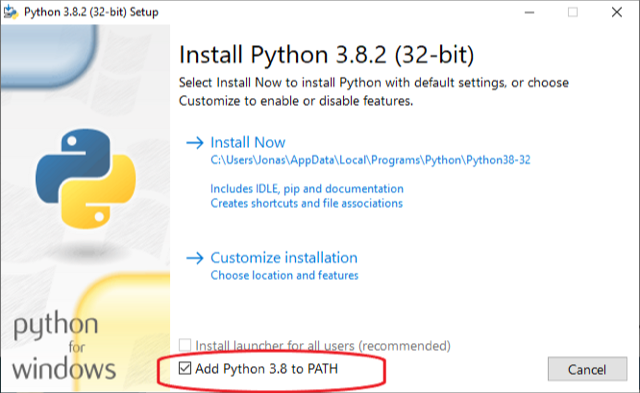
\includegraphics[width=0.8\linewidth,height=0.5\textheight,keepaspectratio]{chapters/06_python1_introduction/figures/python_path.png}
        \end{figure}
    \end{frame}
    
\begin{frame}{Python Interpreter: Windows (II)}
            \textbf{Ausführen des Python-Interpreters:} \\~\
        
Der Python-Interpreter kann auf unterschiedliche Arten geöffnet werden:
        \begin{itemize}
            \item Über das Startmenü \textrightarrow Python3.x
            \item Über die Kommandozeile: 
            \begin{itemize}
                \item{[WIN + R] drücken (oder nach 'Eingabeaufforderung' suchen)}
                \item \code{cmd} eingeben und bestätigen
                \item \code{python} eingeben
            \end{itemize} 
        \end{itemize}
\end{frame}
    
    \begin{frame}{Python Interpreter: Unix (macOS \& Linux)}
        \textbf{Installation:}\\~\
        
        Auf den meisten Unix-Systemen ist bereits eine Python Installation vorhanden. Jedoch handelt es sich dabei i.d.R. um den veralteten Python 2-Interpreter, der nicht mehr unterstützt wird. Daher sollte mind. Python 3.7 installiert werden. \\~\
        Zur Installation des Interpreters muss den Anweisungen des Installationsprogramms gefolgt werden.\\~\
        
        Der Python-Interpreter wird bei der Installation meist automatisch zur Pfad-Variable hinzugefügt. \\~\
        
        \textbf{Ausführen des Python-Interpreters:} \\~\
        
        Der Python-Interpreter kann auf folgende Weise geöffnet werden:
        \begin{itemize}
            \item macOS: Programme \textrightarrow Dienstprogramme \textrightarrow Terminal \textrightarrow \code{python3} eingeben
            \item Linux: Terminal öffnen \textrightarrow \code{python3} eingeben
        \end{itemize}
    \end{frame}
    
    \begin{frame}{Python Interpreter}
        Nachdem der Interpreter geöffnet wurde, sollte folgende (ähnliche) Ausgabe erscheinen:
        
        \begin{figure}
            \centering
            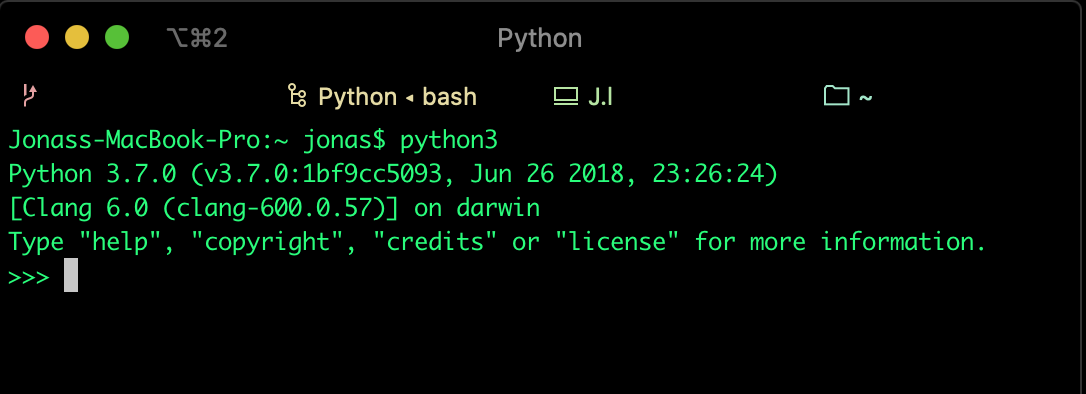
\includegraphics[width=0.8\linewidth,height=0.5\textheight,keepaspectratio]{chapters/06_python1_introduction/figures/interpreter.png}
            \caption{Der Python-Interpreter auf macOS}
        \end{figure}
    \end{frame}
    
    \begin{frame}{Python Interpreter}
        Eine Möglichkeit, Python-Code auszuführen, ist, den Code direkt in die Interpreter-Umgebung einzugeben. Hier wird der Code umgehend ausgeführt und die Ausgabe dem Nutzer angezeigt. \\~\
        
        Dass sich der Nutzer im Interpreter befindet, erkennt er daran, dass die Eingabezeile mit \code{>>>} beginnt. \\~\
        
        Diese Umgebung wird auch als \textbf{REPL} (Read-eval-print loop) bezeichnet, da hier kontinuierlich Befehle vom Nutzer eingelesen, verarbeitet und die Ergebnisse wieder ausgegeben werden. \\~\
        
        Eine weitere Möglichkeit, den Code auszuführen, besteht darin, dem Python-Interpreter den Pfad zu einer Python-Datei zu übergeben. Diese Methode wird später vorgestellt.
    \end{frame}
    
    \begin{frame}[fragile]{Schließen des Interpreters}
        Um den Interpreter-Modus zu beenden und in den normalen Kommandozeilenmodus zurückzukehren (bzw. das Fenster zu schließen, falls der Interpreter nicht über die Kommandozeile geöffnet wurde), gibt es zwei Befehle, die genutzt werden können:
        
\begin{pyconcode}
>>> exit()
\end{pyconcode}

und

\begin{pyconcode}
>>> quit()
\end{pyconcode}
    \end{frame}
    
    
    \begin{subsection}{Aufgaben}
    
        \begin{frame}{Aufgaben}
            \begin{enumerate}
                \item Öffnen Sie den Python-Interpreter. Überprüfen Sie, ob der Python-Interpreter ordnungsgemäß geöffnet wurde. Falls nicht, versuchen Sie das Problem zu lösen.
                
                \item Öffnen Sie den Python-Interpreter und schließen Sie diesen wieder, indem Sie einen Befehl eingeben.
            \end{enumerate}    
        \end{frame}
    
    \end{subsection}
%\newcommand{\decktitle}{Python II - Grundlagen}

%%%%%%%%%%%%%%%%%%%%%%%%%%%%%%%%%%%%%%%%%%%%%%%%%
%
% DOCUMENT
%
%%%%%%%%%%%%%%%%%%%%%%%%%%%%%%%%%%%%%%%%%%%%%%%%%

\begin{frame}
    \subtitle{\decktitle}
    \titlepage
\end{frame}


\begin{frame}
    \frametitle{\textbf{Outline:}}
    \tableofcontents
\end{frame}

		
        
    \section{Variablen}
    
        \begin{frame}[fragile]{Variablen - Deklaration}
            In Python ist kein spezieller Befehl nötig, um Variablen zu erzeugen und zu deklarieren. Es muss lediglich festgelegt werden, wie der Name der Variable lautet und welcher Wert ihr zugewiesen wird. \\~\

\begin{pyconcode}
>>> x = 1
>>> y = 3.14
>>> z = "Hello world"
\end{pyconcode}
    
            In obigen Beispiel wurden 3 Variablen mit den Namen $x$, $y$ und $z$ erzeugt und ihnen jeweils die Werte $1$, $3.14$ und \code{"Hello world"} zugewiesen.
            
        \end{frame}
        
        \begin{frame}[fragile]{Mehrfachzuweisung}
            Auf der linken Seite der Variablenzuweisung steht immer der Variablenname, dann folgt ein \code{=}-Zeichen und auf der rechten Seite wird der Wert festgelegt. \\~\
            
            In Python folgt nach jeder Anweisung eine neue Zeile, Folgendes ist also nicht erlaubt: 
\begin{pyconcode}
>>> x = 1, y = 3.14
\end{pyconcode}

            Es können jedoch trotzdem mehrere Variablen innerhalb einer Zeile deklariert werden \textit{(Multiple Assignment)}:
\begin{pyconcode}
>>> x, y = 1, 3.14
\end{pyconcode}
            
            Auf diese Weise wird ebenso wie oben der Variable \code{x} der Wert \code{1} und der Variable \code{y} der Wert \code{3.14} zugewiesen
            
        \end{frame}
        
        \begin{frame}[fragile]{Wertüberschreibung}
        
            Nachdem einer Variablen ein Wert zugewiesen wurde, kann diese im Anschluss ohne Umstände auch mit einem anderen Wert überschrieben werden:
  
\begin{pyconcode}
>>> x = 1
>>> x = 5
>>> x
5
\end{pyconcode}
            Der Variablen \code{x} wurde zunächst der Wert \code{1} zugewiesen und anschließend mit dem Wert \code{5} überschrieben. \code{x} besitzt nun also den Wert \code{5}. 
            Eine Variable kann auch mit einem Wert eines anderen Datentyps überschrieben werden:

\begin{pyconcode}
>>> x = 1
>>> x = "Hello world"
>>> x
"Hello world"
\end{pyconcode}

        \end{frame}
        
        \begin{frame}[fragile]{Ausgabe}
            Um sich den aktuellen Wert einer Variablen anzeigen zu lassen, muss im interaktiven Modus des Python-Interpreters lediglich der Name der Variable eingegeben werden, der Wert wird dann als Ausgabe in der nächsten Zeile angezeigt:
\begin{pyconcode}
>>> x = 1
>>> x
1
\end{pyconcode}

            Alternativ kann auch die \code{print()}-Funktion genutzt werden, um Werte auszugeben:
\begin{pyconcode}
>>> x = 1
>>> print(x)
1
\end{pyconcode}

        \end{frame}
        
        \begin{frame}[fragile]{Ausgabe}
            \begin{alertblock}{Achtung}
                Die 1. Methode, bei der lediglich der Variablenname "ausgeführt" wird, funktioniert nur im interaktiven Modus des Interpreters. Wird der Code innerhalb einer Datei o.ä. ausgeführt, muss immer die \code{print()}-Funktion genutzt werden.
            \end{alertblock}
        
        \end{frame}
        
        \begin{frame}{Benamungsregeln \& -konventionen}
            \textbf{Regeln}: Variablennamen
            \begin{itemize}
                \item \textbf{müssen} mit einem Buchstaben oder einem Underscore (\_) beginnen
                \item \textbf{dürfen nicht} mit einer Zahl/Ziffer beginnen
                \item \textbf{dürfen lediglich} aus alphanumerischen Zeichen (A-Z, a-z, 0-9) und Underscores (\_) bestehen
                \item sind case-sensitive (Groß-/ Kleinschreibung wird unterschieden, z.B. $x \neq X$)
            \end{itemize}
            
            \textbf{Konventionen}: Variablennamen
            \begin{itemize}
                \item \textbf{sollten} möglichst aussagekräftig sein (z.B. ist der Variablenname \code{x} kaum aussagekräftig, \code{age} dagegen schon)
                \item bestehen i.d.R. nur aus Kleinbuchstaben, wobei einzelne Wörter durch Underscores getrennt werden (z.B. \code{age\_of\_person}), wird als \textit{Snake case (snake\_case)} bezeichnet\footnote{In manchen anderen Programmiersprachen (z.B. Java) wird überwiegend \textit{Camel case (camelCase)} genutzt, wobei Wörter nicht durch Underscores getrennt werden, sondern der erste Buchstabe eines Wortes groß geschrieben wird (z.B. \texttt{ageOfPerson})}
            \end{itemize}
        \end{frame}
        
        \begin{subsection}{Aufgaben}
            
            \begin{frame}{Aufgaben}
            
                \begin{enumerate}
                    \item Wie werden in Python Variablen erzeugt?
                    \item Wie können den Variablen \code{name} und \code{age} innerhalb einer Zeile verschiedene Werte zugewiesen werden?
                    \item Sind Variablenwerte konstant? Wie können sie verändert werden?
                    \item Welche der folgenden Variablennamen sind valide?
                        \begin{itemize}
                            \item \texttt{\_name}
                            \item \texttt{name\_}
                            \item \texttt{Name}
                            \item \texttt{int}
                            \item \texttt{int\$}
                            \item \texttt{name\_and\_age}
                            \item \texttt{nameAndAge}
                            \item \texttt{name and age}
                            \item \texttt{1variable}
                            \item \texttt{variable1}
                        \end{itemize}
                    \item Was muss bei der Ausgabe von Werten im interaktiven Interpreter bzw. der Ausführung des Codes in Dateien beachtet werden?
                    \item Wie sollten Variablen in Python benamt werden?
                \end{enumerate}
                
            \end{frame}
        \end{subsection}
        
    \section{Kommentare}
        \begin{frame}{Kommentare (I)}
            Wie in den meisten anderen Programmiersprachen besteht in Python die Möglichkeiten, den Code mit Kommentaren anzureichern. \\~\
            
            Kommentare dienen dazu, Informationen im Code zu ergänzen, um beispielsweise die Funktionalität zu beschreiben bzw. dokumentieren, anderen Entwicklern eine Hilfestellung zu geben, den Code besser verstehen zu können oder auch komplexe Sachverhalte in natürlicher Sprache wiederzugeben, die in Codeform nur schwer verständlich sind. \\~\

            Kommentare werden vom Interpreter nicht berücksichtigt, daher können Kommentare einen beliebigen Inhalt besitzen.
        \end{frame}
        
        \begin{frame}[fragile]{Kommentare (II) - Einzeilige Kommentare}
            
            Kurze Kommentare werden mit einem \code{\#}-Zeichen vorangestellt. Diese Kommentare gelten nur bis zum jeweiligen Zeilenende.

\begin{pythoncode}
# Das ist ein Kommentar.            
x = 1 #  Das ist ein Kommentar, der erst nach der Variablenzuweisung beginnt
\end{pythoncode}
        \end{frame}
        
        \begin{frame}[fragile]{Kommentare (III) - Mehrzeilige Kommentare}
            
            Manchmal (insbesondere bei der Beschreibung komplexer Sachverhalte) können sich Kommentare auch über viele Zeilen erstrecken. Um nicht explizit jede Zeile mit \code{\#} voranstellen zu müssen, gibt es in Python die Möglichkeit, mehrzeilige Kommentare zu erzeugen.
            
            Mehrzeilige Kommentare werden mit 3 Anführungszeichen (\code{"""}) eingeleitet und auch wieder beendet.
            Alles was dazwischen enthalten ist wird als Kommentar behandelt und vom Interpreter ignoriert.
\begin{pythoncode}
"""
Das ist ein mehrzeiliger Kommentar.

Alles was zwischen den Anführungszeichen steht wird vom Interpreter ignoriert.
Hier ist der Kommentar beendet
"""
\end{pythoncode}
        \end{frame}
    
    \section{Datentypen}
    
        \begin{frame}{Datentypen}
            Da Python eine typisierte Sprache ist, besitzt jede Variable auch einen Datentypen. Datentypen beschreiben, welche Art von Wert in einer Variablen gespeichert ist. \\~\
            
            \begin{block}{Hinweis}
                Um zu überprüfen, welchen Datentypen eine Variable besitzt, gibt es in Python die \code{type()}-Funktion. Um bspw. den Datentypen der Variablen \code{x} festzustellen, kann die Funktion folgendermaßen aufgerufen werden: \code{type(x)}
            \end{block}
        \end{frame}
        
        \begin{frame}[fragile]{Numerische Datentypen (I)}
            
            Numerische Datentypen beschreiben Zahlenwerte unterschiedlicher Art:
            
            \begin{itemize}
                \item \textbf{integer}: Positive und negative Ganzzahlen (keine Nachkommastellen). \\~\
                Bezeichnung in Python: \textbf{\code{int}}
\begin{pyconcode}
>>> x = 5
>>> type(x)
<class 'int'>
\end{pyconcode}
            
                \item \textbf{float}: Positive und negative reelle Zahlen mit Fließkommadarstellung (mit Nachkommastellen). \\~\
                Bezeichnung in Python: \textbf{\code{float}}
\begin{pyconcode}
>>> x = 3.14
>>> type(x)
<class 'float'>
\end{pyconcode}

            \end{itemize}
        \end{frame}
        
        
        \begin{frame}[fragile]{Numerische Datentypen (II)}
        
            \begin{itemize}
                \item \textbf{complex}:Komplexe Zahlen mit einem reellen und einem imaginären Anteil. Sowohl der reelle als auch der komplexe Anteil wird durch \code{float}-Zahlen dargestellt. In der Ausgabe wird der imaginäre Teil durch ein \code{j} gekennzeichnet, um deutlich zu machen, dass es sich dabei um eine imaginäre Zahl handelt. Im Beispiel unten wird eine komplexe Zahl mit dem reellen Anteil \code{1} und dem imaginären Anteil \code{0} erzeugt. \\~\
                Bezeichnung in Python: \textbf{\code{complex}}
\begin{pyconcode}
>>> x = complex(1,0)
>>> x
(1+0j)
>>> type(x)
<class 'complex'>
\end{pyconcode}
            \end{itemize}
            
        \end{frame}
        
         \begin{frame}[fragile]{Numerische Datentypen (III)}
            \begin{alertblock}{Achtung}
                Bei der Verwendung von Kommazahlen muss auf die korrekte Verwendung des Dezimaltrennzeichens geachtet werden. Da die Schreibweisen in der Informatik meist auf dem englischen System basieren, wird als Dezimaltrennzeichen ein Punkt und kein Komma verwendet (z.B. \code{3.14} anstatt \code{3,14}).
            \end{alertblock}
         \end{frame}
        
        
        \begin{frame}[fragile]{Boolesche Datentypen}
        
            \begin{itemize}
                \item \textbf{boolean}: Benannt nach George Boole. Stellt einen einfachen Zustandswert dar. Es gibt lediglich zwei Zustände: Wahr und Falsch (analog: Binärdarstellung (1 / 0), Schalterdarstellung (An / Aus)). \\~\
                Bezeichnung in Python: \textbf{\code{bool}}
\begin{pyconcode}
>>> x = True
>>> y = False
>>> type(x)
<class 'bool'>
>>> type(y)
<class 'bool'>
\end{pyconcode}

            \begin{alertblock}{Achtung}
                \code{True} und \code{False} sind eingebaute Schlüsselwörter in Python und daher case-sensitive. \code{true} bzw. \code{false} sind keine validen booleschen Werte.
            \end{alertblock}
            
            \end{itemize}
            
        \end{frame}
        
        \begin{frame}[fragile]{Zeichenketten (I)}
        
            \begin{itemize}
                \item \textbf{string}: Zeichenketten, meist \textit{strings} genannt, sind eine Folge von einzelnen Zeichen, Buchstaben und Ziffern, die als Buchstaben behandelt werden, die von einfachen (\code{'}) oder doppelten (\code{"}) Anführungszeichen eingeschlossen werden.\\~\
                Bezeichnung in Python: \textbf{\code{str}}
\begin{pyconcode}
>>> x = 'Hello world'
>>> type(x)
<class 'str'>
>>> y = "1234"
>>> type(y)
<class 'str'>
\end{pyconcode}

            \begin{alertblock}{Achtung}
                Ein String wird entweder von einfachen oder doppelten Anführungszeichen eingeschlossen, eine Kombination innerhalb eines Strings ist aber \textbf{nicht} erlaubt (z.B. \code{"Hello world'})
            \end{alertblock}
            
            \end{itemize}
            
        \end{frame}
        
        \begin{frame}[fragile]{Zeichenketten (II)}
            Zeichenketten müssen nicht zwangsläufig statisch angelegt werden, sondern können auch dynamisch erzeugt werden, d.h. mit den Werten anderer Variablen ergänzt werden.\\~\
            
            
            Hierfür können sogenannte \textbf{f-Strings} verwendet werden. Um diese zu nutzen, muss die Zeichenkette mit einem "f" ("formatiert") vorangestellt werden. Variablenwerte, die in den String eingefügt werden sollen, werden innerhalb des Strings mit geschweiften Klammern (\code{\{\}}) injiziert.
\begin{pythoncode}
>>> first_name = 'John'
>>> age = 42

>>> print(f"Hallo {first_name}, du bist {age} Jahre alt")
"Hallo John, du bist 42 Jahre alt"
        
\end{pythoncode}
        
        \end{frame}
        
        \begin{frame}[fragile]{Zeichenketten (III)}
        Alternativ können Zeichenketten auch mit einen \code{+}-Zeichen konkateniert (zusammengesetzt) werden.
        
        \begin{alertblock}{Achtung}
                String-Konkatenation mithilfe des Addition-Operators funktioniert nur zwischen Strings, andere Datentypen müssen vor der Konkatenation zunächst in den String-Datentyp konvertiert werden.
            \end{alertblock}
\begin{pythoncode}
>>> first_name = 'John'
>>> age = 42

>>> print("Hallo " + first_name + ", du bist " + age +  " Jahre alt")
TypeError: can only concatenate str (not "int") to str

>>> print("Hallo " + first_name + ", du bist " + str(age) +  " Jahre alt")
"Hallo John, du bist 42 Jahre alt"
        \end{pythoncode}       
            
        
        \end{frame}
        
        \begin{frame}[fragile, allowframebreaks]{Zeichenketten (IV)}
            Zur Zeichenkettenverarbeitung stehen weitere Funktionen zur Verfügung, die bereits standardmäßig in Python enthalten sind sind.
            
            \begin{itemize}
                \item \code{upper()}: Wandelt String in Großbuchstaben um (analog dazu: \code{lower()})
\begin{pythoncode}
>>> "Hello".upper()
"HELLO"
\end{pythoncode}
                \item \code{startswith()}: Überprüft, ob ein String mit einer bestimmten Zeichenkette beginnt und liefert dementsprechend einen booleschen Wert zurück (analog dazu: \code{endswith()})
\begin{pythoncode}
>>> "Hello John".startswith("Hello")
True
\end{pythoncode}

                \item \code{split()}: Trennt einen String anhand der gewünschten Zeichen und gibt die Bestandteile als Liste zurück. Falls kein Parameter angegeben wird, wird standardmäßig anhand von Leerzeichen getrennt
\begin{pythoncode}
>>> "Hello John".split()
["Hello", "John"]

>>> "This.sentence.is.dot.separated".split(".")
['This', 'sentence', 'is', 'dot', 'separated']
\end{pythoncode}
            \end{itemize}
            
In Python stehen viele weitere String-Funktionen zur Verfügung. Eine vollständige Beschreibung dieser Funktionen kann in der \href{https://docs.python.org/3/library/stdtypes.html#string-methods}{offiziellen Dokumentation} eingesehen werden.
        \end{frame}
        
        \begin{frame}[fragile]{None}
            
            Um zu kennzeichnen, dass eine Variable existiert, diese jedoch keinen Wert beinhaltet, also \textit{leer} ist, gibt es den Datentyp und das Schlüsselwort \code{None}.\\~\
            
            \begin{alertblock}{Achtung}
                \code{None} besitzt eine andere semantische und logische Bedeutung als der Wert \code{0}. \code{0} bedeutet, dass ein Wert vorhanden ist, dieser aber \texttt{0} beträgt, also einen numerischen Wert trägt. \code{None} dagegen bedeutet, dass überhaupt kein Wert gesetzt ist, daher handelt es sich auch nicht um einen numerischen Datentyp.
            \end{alertblock}

\begin{pyconcode}
>>> x = None
>>> type(x)
<class 'NoneType'>
>>> print(x)
None
>>> x is None
True
>>> x == None
True
>>> x == 0
False
\end{pyconcode}            
            
         \end{frame}
        
         \begin{frame}[fragile]{Weitere Datentypen}
            
            \begin{itemize}
                \item \textbf{Sequence} Datentypen: Sammlung mehrerer Werte (gleicher oder unterschiedlicher Datentypen) innerhalb einer Variable, z.B. \code{list}, \code{tuple}, \code{range}
                
                \item \textbf{Mapping} Datentypen: Sammlung mehrerer Werte (gleicher oder unterschiedlicher Datentypen) nach dem Key-Value Prinzip, z.B. \code{dict} (Dictionary/Wörterbuch)
                
                \item \textbf{Set} Datentypen: Sammlung mehrerer Werte (gleicher oder unterschiedlicher Datentypen) ohne Duplikate innerhalb einer Variable, z.B. \code{set}
                
                \item \textbf{Binäre} Datentypen: Darstellung von Zahlen im Binärsystem, z.B. \code{bytes}.
            \end{itemize}\\~\
            
            Sequence, Mapping und Set Datentypen werden im Abschnitt \nameref{subs:datastruct} näher erläutert, binäre Datentypen werden in diesem Rahmen nicht besprochen.
         \end{frame}
         
         
        \begin{frame}[fragile]{Konvertierungen (I)}
            Da Python schwach typisiert ist, können Variablen prinzipiell ohne weiteres in andere Datentypen umgewandelt werden. Hierfür stehen bereits standardmäßig Funktionen zu Verfügung, die genutzt werden können:
            
            \begin{table}[]
                \begin{tabular}{|l|c|c|c|c|c|}
                    \hline
                    \rowcolor[HTML]{EFEFEF} 
                    Umwandlung in ...                & Integer & Float   & Complex   & Boolescher Wert & String \\ \hline
                    \cellcolor[HTML]{EFEFEF}Funktion & int()   & float() & complex() & bool()          & str()  \\ \hline
                \end{tabular}
            \end{table}
            
\begin{pyconcode}
>>> x = 5
>>> type(x)
<class 'int'>
>>> y = float(x)
>>> type(y)
<class 'float'>
>>> y
5.0
\end{pyconcode}
        \end{frame}
    
        \begin{frame}[fragile]{Konvertierungen (II)}
            
            Bei Typkonvertierungen muss immer darauf geachtet werden, ob die Konvertierung \colorbox{good}{problemlos möglich} ist, u.U. mit \colorbox{medium}{Datenverlust oder Fehlern} gerechnet werden muss oder grundsätzlich \colorbox{bad}{nicht möglich} ist.
   
           \begin{table}[]
                \centering
                \resizebox{\textwidth}{!}{%
                \begin{tabular}{|l|c|c|c|c|c|}
                    \hline
                    \cellcolor[HTML]{EFEFEF} \diagbox{Von...}{zu...}
                    &
                    \multicolumn{1}{l|}{\cellcolor[HTML]{EFEFEF}int}
                    & 
                    \multicolumn{1}{l|}{\cellcolor[HTML]{EFEFEF}float}
                    & 
                    \multicolumn{1}{l|}{\cellcolor[HTML]{EFEFEF}complex}                     & 
                    \multicolumn{1}{l|}{\cellcolor[HTML]{EFEFEF}bool}                        & 
                    \multicolumn{1}{l|}{\cellcolor[HTML]{EFEFEF}str}                         \\ \hline


%% int row
\cellcolor[HTML]{EFEFEF}int     &                                                           

\cellcolor[HTML]{9AFF99} & 

\cellcolor[HTML]{9AFF99} \begin{tabular}[c]{@{}c@{}}Zahl besitzt zusätzlich\\ Dezimalstelle\\ \\ \code{float(5)} \Rightarrow \code{5.0}\end{tabular} & 

\cellcolor[HTML]{9AFF99} \begin{tabular}[c]{@{}c@{}}Integerzahl als reelle Zahl,\\ kein imaginärer Anteil\\ \\ \code{complex(5)} \Rightarrow \code{(5+0j)}\end{tabular} &

\cellcolor[HTML]{9AFF99} \begin{tabular}[c]{@{}c@{}}0 wird zu \code{False} ausgewertet,\\ alle anderen Zahlen zu \code{True}\\ \\ \code{bool(5)} \Rightarrow \code{True}\\ \code{bool(0)} \Rightarrow \code{False}\end{tabular} & 

\cellcolor[HTML]{9AFF99} \begin{tabular}[c]{@{}c@{}}String mit der Zahl als Inhalt\\ \\ \code{str(5)} \Rightarrow \code{'5'}\end{tabular}                                           

\\ \hline

% float row
\cellcolor[HTML]{EFEFEF}float   & 

\cellcolor[HTML]{FFFE65}\begin{tabular}[c]{@{}c@{}}Datenverlust, falls Zahl einen \\ Nachkommawert $\neq 0$ hat \\ (Nachkommastellen werden abgeschnitten) \\ \\ \code{int(5.0)} \Rightarrow \code{5}\\ \code{int(5.9)} \Rightarrow \code{5}\end{tabular} &                  

\cellcolor[HTML]{9AFF99} & 

\cellcolor[HTML]{9AFF99} \begin{tabular}[c]{@{}c@{}}Floatzahl als reelle Zahl,\\ kein imaginärer Anteil\\ \\ \code{complex(5.0)} \Rightarrow \code{5.0+0j}\end{tabular} & 

\cellcolor[HTML]{9AFF99} \begin{tabular}[c]{@{}c@{}}0.0 wird zu \code{False} ausgewertet,\\ alle anderen Zahlen zu \code{True}\\ \\ \code{bool(5.0)} \Rightarrow \code{True}\\ \code{bool(0.0)} \Rightarrow \code{False}\end{tabular} & 

\cellcolor[HTML]{9AFF99} \begin{tabular}[c]{@{}c@{}}String mit der Zahl als Inhalt\\ \\ \code{str(5.0)} \Rightarrow \code{'5.0'}\end{tabular}                                                             
\\ \hline

% complex row
\cellcolor[HTML]{EFEFEF}complex & 

\cellcolor[HTML]{FD6864}nicht möglich &

\cellcolor[HTML]{FD6864}nicht möglich &

\cellcolor[HTML]{9AFF99} & 

\cellcolor[HTML]{9AFF99} \begin{tabular}[c]{@{}c@{}}Wenn sowohl der reelle als auch der imaginäre Teil 0 ist,\\ wird der Ausdruck zu \code{True} ausgewertet,\\ ansonsten zu \code{False}\\ \\ \code{bool(complex(5,0))} \Rightarrow \code{True}\\ \code{bool(complex(0,0))} \Rightarrow \code{False}\end{tabular} &

\cellcolor[HTML]{9AFF99}\begin{tabular}[c]{@{}c@{}}String mit der komplexen Zahl als Inhalt\\ \\ \code{str(complex(5,2))} \Rightarrow \code{'(5+2j)'}\end{tabular}                                       

\\ \hline

% bool row

\cellcolor[HTML]{EFEFEF}bool    & 

\cellcolor[HTML]{9AFF99} \begin{tabular}[c]{@{}c@{}}\code{True} wird zu \code{1} ausgewertet,\\ \code{False} zu \code{0}\\ \\ \code{int(True)} \Rightarrow \code{1}\\ \code{int(False)} \Rightarrow \code{0}\end{tabular} &

\cellcolor[HTML]{9AFF99} \begin{tabular}[c]{@{}c@{}}\code{True} wird zu \code{1.0} ausgewertet,\\ \code{False} zu \code{0.0}\\ \\ \code{float(True)} \Rightarrow \code{1.0}\\ \code{float(False)} \Rightarrow \code{0.0}\end{tabular} &

\cellcolor[HTML]{9AFF99} \begin{tabular}[c]{@{}c@{}}\code{True} wird zu \code{1.0+0j} ausgewertet,\\ \code{False} zu \code{0.0+0j}\\ \\ \code{complex(True)} \Rightarrow \code{1.0+0j}\\ \code{complex(False)} \Rightarrow \code{0.0+0j} \Rightarrow \code{0j}\end{tabular}  &    

\cellcolor[HTML]{9AFF99} & 

\cellcolor[HTML]{9AFF99} \begin{tabular}[c]{@{}c@{}}String mit dem booleschen Wert als Inhalt\\ \\ \code{str(True)} \Rightarrow \code{'True'}\\ \code{str(False)} \Rightarrow \code{'False'}\end{tabular} 

\\ \hline

% str row
\cellcolor[HTML]{EFEFEF}str     & 

\cellcolor[HTML]{FFFE65} \begin{tabular}[c]{@{}c@{}}Fehler, falls String einen nicht-numerischen Wert enthält \\ \\ \code{int('5')} \Rightarrow \code{5}\\ \code{int('hello')} \Rightarrow \code{Error}\end{tabular} &

\cellcolor[HTML]{FFFE65} \begin{tabular}[c]{@{}c@{}}Fehler, falls String einen nicht-numerischen Wert \\ (exkl. Dezimaltrennzeichen) enthält \\ \\ \code{float('5.0')} \Rightarrow \code{5.0}\\ \code{float('5.hello')} \Rightarrow \code{Error}\end{tabular} &

\cellcolor[HTML]{FFFE65} \begin{tabular}[c]{@{}c@{}}Fehler, falls String nicht der Darstellung einer komplexen Zahl entspricht\\ oder der String Leerzeichen enthält\\ \\ \code{complex('5+2j'} \Rightarrow \code{5+2j}\\ \code{complex('5')} \Rightarrow \code{5+0j}\\ \code{complex('5 + 2j')} \Rightarrow \code{Error}\end{tabular} &

\cellcolor[HTML]{FFFE65} \cellcolor[HTML]{9AFF99}\begin{tabular}[c]{@{}c@{}}Leerer String wird zu \code{False} ausgewertet,\\ alle anderen Strings zu \code{True}\\ \\ \code{bool('hello world')} \Rightarrow \code{True}\\ \code{bool('')} \Rightarrow \code{False}\end{tabular} & 

\cellcolor[HTML]{9AFF99}                                                                                                                                                         \\ \hline
\end{tabular}%
}
\end{table}
        \end{frame}
        
        \begin{subsection}{Aufgaben}
            \begin{frame}[fragile]{Aufgaben}
                \begin{enumerate}
                    \item Ist Python eine typisierte oder typenlose Sprache?
                    \item Ist Python stark oder schwach typisiert?
                    \item Mit welcher Funktion kann der Typ einer Variablen überprüft werden?
                    \item Welche numerischen Datentypen gibt es und worin unterscheiden sie sich?
                    \item Was muss bei der Dezimaldarstellung von Zahlen beachtet werden?
                    \item Wofür werden boolesche Datentypen genutzt?
                    \item Können die Datentypen ineinander umgewandelt werden? Was ist dabei zu beachten? Wie lauten die Funktionen?
                    \item Was ist das Ergebnis folgender Umwandlungen?:
\begin{pyconcode}
>>> float(50)
>>> str(50)
>>> int(complex(3,1))
>>> complex("3+ 1j")
>>> str('int')
>>> bool(3.14)
\end{pyconcode}                     
                \end{enumerate}
            \end{frame}
        \end{subsection}
    
    \section{Mathematische Operationen}
        
        \begin{frame}[fragile]{Grundrechenarten}
            Mithilfe von Python können unterschiedlichste mathematische Operationen durchgeführt werden. Dazu gehören z.B. die Grundrechenarten Addition, Subtraktion, Multiplikation und Division:
        
\begin{pyconcode}
>>> x = 10
>>> y = 5
>>> x + y
15
>>> x - y
5
>>> x * y
50
>>> x/y
5.0
\end{pyconcode}        
        \end{frame}
        
        
        \begin{frame}[fragile]{Grundrechenarten (II)}
            
            \begin{block}{Beachte}
                Falls die Rechenoperation lediglich aus Integerwerten besteht, ist auch das Ergebnis der Addition, Subtraktion und Multiplikation stets ein Integerwert. Lediglich bei der Division kann das Ergebnis eine Fließkommazahl sein, sodass der Datentyp einer Division von zwei Integerwerten immer ein Floatwert ist. \\~\
                Bei Operationen mit Floatwerten ist das Ergebnis immer ein Floatwert, unabhängig von der Rechenart.
            \end{block}
        \end{frame}
        
         \begin{frame}[fragile]{Weitere Rechenoperationen (I)}
            
            Neben den Grundrechenarten sind in Python auch weitere Rechenoperationen möglich:
            
              \begin{itemize}
                \item Modulo: Berechnet den Dezimalpart eines Quotienten ("Rest einer Division"). Operator: \code{\%}
                 
\begin{pyconcode}
>>> x = 10
>>> y = 4
>>> x / y
2.5
>>> x % y
2
\end{pyconcode}                   
                
                \item Potenz: Eine Potenz wird durch zwei Multiplikationszeichen dargestellt. Davor befindet sich die Basis, dahinter der Exponent. Operator: \code{**}

\begin{pyconcode}
>>> 2 ** 4
16
>>> 5 ** 0
1
\end{pyconcode}                   
                
            \end{itemize}
        \end{frame}

        \begin{frame}[fragile]{Weitere Rechenoperationen (II)}
             \begin{itemize}
                \item Integer-Division: Rundet den Quotienten auf den nächsten Integerwert ab. Operator: \code{//}
                 
\begin{pyconcode}
>>> x = 9
>>> y = 2
>>> x / y
4.5
>>> x // y
4
\end{pyconcode}     
                \item Weitere (komplexere) mathematische Funktionen wie \code{sin()}, \code{abs()}, \code{round()}, ... werden durch das \texttt{math}-Modul bereitgestellt.
            \end{itemize}
        \end{frame}
        
        \begin{frame}[fragile, allowframebreaks]{Kurzschreibweise}
            Falls dem Wert einer Variablen \code{x} ein beliebiger anderer Wert hinzuaddiert werden soll und das Ergebnis wiederum der Variablen \code{x} zugewiesen werden soll, so kann dies in Python ausgedrückt werden mit:
\begin{pythoncode}
>>> x = 5
>>> x = x + 2 # Der Variablen x wird 2 hinzuaddiert und das Ergebnis der Variablen x zugewiesen
\end{pythoncode}

        Für diese Operation existiert in Python eine Kurzschreibweise, die häufig genutzt wird:
\begin{pythoncode}
>>> x = 5
>>> x += 2 # Der Variablen x wird 2 hinzuaddiert und das Ergebnis der Variablen x zugewiesen, äquivalent zu obiger Schreibweise
\end{pythoncode}

        Diese Kurzschreibweise ist nicht nur auf Additionen anwendbar, sondern auf alle weiteren mathematischen Operationen:
\begin{pythoncode}
>>> x = 5
>>> x %= 2 # Entspricht x = x % 2
>>> print(x)
1

>>> x = 5
>>> x *= 2
>>> print(x)
10
\end{pythoncode}
        \end{frame}
        
        
        \begin{frame}[fragile]{Ausführungsreihenfolge}
            Die Ausführungsreihenfolge ("\textit{Order of operations}") ist identisch zur mathematischen Reihenfolge nach dem \textcolor{blue}{PEMDAS}-Prinzip:
            
            \begin{enumerate}
                \item \textcolor{blue}{P}arantheses (Klammern)
                \item \textcolor{blue}{E}xponents (Potenzen, Wurzeln, Logarithmen, ...)
                \item \textcolor{blue}{M}ultiplikation \& \textcolor{blue}{D}ivision
                \item \textcolor{blue}{A}ddition \& \textcolor{blue}{S}ubstraktion
            \end{enumerate} \\~\
            
            Bei Operationen gleicher Präzedenz (Operatorrangfolge) (z.B. Multiplikation und Division) wird von links nach rechts ausgewertet.
            
        \end{frame}
        
        \begin{frame}[fragile]{Exkursion: Fließkomma-Arithmetik (I)}
\begin{pyconcode}
>>> 10/3
3.3333333333333335
\end{pyconcode}     

        Woher kommt die 5 am Ende der Fließkommazahl? \\~\
        
        Dieses Problem entsteht aus der Fließkomma-Arithmetik beim Dividieren von Zahlen.
        Zahlen werden im Computer grundsätzlich durch Binärzahlen dargestellt. Da das binäre System aber lediglich aus Ganzzahlen (0, 1, 2, 4, 8, ...) besteht, müssen Kommazahlen durch Divisionen der Binärzahlen abgebildet werden. Beispielsweise kann die Zahl \code{0.125} aus \code{1/8} gebildet werden. \code{0.75} kann dagegen aus \code{1/2 +  1/4} gebildet werden.
        
        
        
        \end{frame}
        
        \begin{frame}[fragile]{Exkursion: Fließkomma-Arithmetik (II)}
            
             Da \code{10/3} jedoch eine Zahl mit unendlich vielen Nachkommastellen darstellt, wären auch unendlich viele Summanden notwendig, um die Zahl korrekt darzustellen. Da dies nicht  möglich ist, wird versucht, sich der Zahl so genau wie möglich anzunähern, eine Restungenauigkeit bleibt jedoch immer. \\~\
             
             Hinzu kommt, dass innerhalb einer Variable nur begrenzt viel Platz zur Verfügung steht (32 bzw. 64 Bit), aus diesem Grund wird die Zahl abgeschnitten, sobald die maximale Länge erreicht ist. Auch hierzu kommt es also zu einer kleinen Ungenauigkeit ($ 3 < 3.3 < 3.33 < 3.333 < ...$).\\~\
             
             Python rechnet intern mit der Zahl \code{3.3333333333333334813630699500208720564842224121094}, diese wird aber zur besseren Lesbarkeit in der Ausgabe gekürzt und gerundet, sodass die Zahl \code{3.3333333333333335} angezeigt wird.
             
        \end{frame}
        
        \begin{subsection}{Aufgaben}
        
            \begin{frame}{Aufgaben}
                \begin{enumerate}
                    \item Welchen Datentyp hat eine Addition, Subtraktion, Multiplikation und Division von Integer-, Float- und Complex-Werten
                    \item Was ist eine Modulorechnung und was ist der entsprechende Operator?
                    \item Wie wird der Term $3^{-5}$ in Python ausgedrückt?
                    \item Wofür kann die Integer-Division nützlich sein?
                    \item Wie geht der Entwickler vor, wenn er bspw. eine Sinusberechnung durchführen muss?
                    \item Wofür steht PEMDAS und wo wird es angewendet?
                    \item Warum werden manche Zahlen ungenau angezeigt? Worin liegt das Grundproblem?
                \end{enumerate}
            \end{frame}
        \end{subsection}
        
        
    \section{Boolesche Operationen}
    
        \begin{frame}[fragile]{Boolesche Operationen}
            Boolesche Werte (\code{True} und \code{False}) können genutzt werden, um Vergleiche anzustellen und Aussagen auf ihren Wahrheitswert zu überprüfen. \\~\
            
            Hierfür sind die Wahrheitstabellen der Aussagenlogik relevant. \\~\
            
            Es gibt unterschiedliche logische Verknüpfungen, zunächst werden die Verknüpfungen basierend auf zwei booleschen Werten betrachtet.
            
        \end{frame}
        
        \begin{frame}[fragile]{AND-Verknüpfung}
            \begin{table}[]
            \centering
                \begin{tabular}{|c|c|c|}
                    \hline
                    \rowcolor[HTML]{EFEFEF} 
                    Wert 1 & Wert 2 & Ergebnis (AND) \\ \hline
                    True   & True   & True           \\ \hline
                    True   & False  & False          \\ \hline
                    False  & True   & False          \\ \hline
                    False  & False  & False          \\ \hline
                \end{tabular}%
            \end{table}
            
            Das Ergebnis ist also nur dann \code{True}, wenn \textbf{beide Werte \code{True}}  sind.\\~\
            
            Hierfür steht in Python das Schlüsselwort \code{and} zur Verfügung.
            
\begin{pyconcode}
>>> True and True
True
>>> True and False
False
>>> False and False
False
\end{pyconcode}     


        \end{frame}
        
         \begin{frame}[fragile]{OR-Verknüpfung}
            \begin{table}[]
            \centering
                \begin{tabular}{|c|c|c|}
                    \hline
                    \rowcolor[HTML]{EFEFEF} 
                    Wert 1 & Wert 2 & Ergebnis (OR) \\ \hline
                    True   & True   & True           \\ \hline
                    True   & False  & True          \\ \hline
                    False  & True   & True          \\ \hline
                    False  & False  & False          \\ \hline
                \end{tabular}%
            \end{table}
            
           Das Ergebnis ist also nur dann \code{True}, wenn \textbf{mindestens ein Wert \code{True}}  ist.\\~\
            
            Hierfür steht in Python das Schlüsselwort \code{or} zur Verfügung.
            
\begin{pyconcode}
>>> True or True
True
>>> True or False
True
>>> False or False
False
\end{pyconcode}     

        \end{frame}
        
        
        \begin{frame}[fragile]{XOR-Verknüpfung}
            \begin{table}[]
            \centering
                \begin{tabular}{|c|c|c|}
                    \hline
                    \rowcolor[HTML]{EFEFEF} 
                    Wert 1 & Wert 2 & Ergebnis (XOR) \\ \hline
                    True   & True   & False           \\ \hline
                    True   & False  & True          \\ \hline
                    False  & True   & True          \\ \hline
                    False  & False  & False          \\ \hline
                \end{tabular}%
            \end{table}
            
           Das Ergebnis ist also nur dann \code{True}, wenn \textbf{genau ein Wert \code{True}}  ist.\\~\
            
            Hierfür steht in Python der Operator \code{\^} zur Verfügung.
            
\begin{pyconcode}
>>> True ^ True
False
>>> True ^ False
True
>>> False ^ False
False
\end{pyconcode}     

        \end{frame}
        
        
        \begin{frame}[fragile]{not-Operator}
            
            Auch eine Negierung (Verneinung, Wertumkehr) ist mit booleschen Werten möglich. \\~\
            
            Hierfür steht in Python das Schlüsselwort \code{not} zur Verfügung.
            
\begin{pyconcode}
>>> not True
False
>>> not False
True
\end{pyconcode}     

        \end{frame}
        
         \begin{frame}[fragile]{Verknüpfung der Operationen}
            
            Die Operationen können auch miteinander Verknüpft werden, um komplexere Aussagen zu testen. \\~\
            
\begin{pyconcode}
>>> not ((True and False) or (True and True)) ^ True
True
\end{pyconcode}     

        \end{frame}
        
        \begin{frame}[fragile]{Test auf (Un-)Gleichheit}
            
            Variablenwerte können verglichen werden, um so herauszufinden, ob eine Aussage wahr oder falsch ist. \\~\
            Es kann ebenso wie in der Mathematik sowohl auf Gleichheit als auch auf Ungleichheit getestet werden.
            
        \end{frame}
        
        \begin{frame}[fragile]{Test auf Gleichheit}
        
            Mit dem Test auf Gleichheit kann überprüft werden, ob Variablen einander entsprechen, also den gleichen Wert besitzen. \\~\
            
            \begin{alertblock}{Achtung}
            Um zwei Variablen miteinander zu vergleichen reicht kein einfaches \code{=}, da dieses Zeichen bereits zur Wertzuweisung von Variablen genutzt wird. Daher wird für den Vergleich ein doppeltes Gleichheitszeichen (\code{==}) verwendet.
            \end{alertblock}
            
            
\begin{pyconcode}
>>> x = 5
>>> x == 5
True
>>> "hallo" == "welt"
False
>>> x == 5.0
True
\end{pyconcode}     

        \end{frame}
        
        \begin{frame}[fragile]{Test auf Ungleichheit}
        
            Analog zum Test auf Gleichheit kann ebenso überprüft werden, ob sich Variablenwerte unterscheiden. \\~\
            
            Dabei kann sowohl allgemein auf Ungleichheit (\code{!=}), als auch auf Verhältnisse (\code{>}, \code{<}, \code{>=}, \code{<=}) getestet werden.
            
\begin{pyconcode}
>>> x = 5
>>> x != 4
True
>>> x >= 7
False
>>> "hallo" != "welt"
True
\end{pyconcode}     

        \end{frame}
        
        \begin{frame}[fragile]{Verknüpfung der Operationen}
            
            Nun lassen sich alle booleschen Operationen (Verknüpfung, Negierung, Gleichheit, Ungleichheit) miteinander verbinden\\~\
            
\begin{pyconcode}
>>> x>=5 and x<=10 ^ (not 5<10)
True
\end{pyconcode}     

        \end{frame}
        
        \begin{frame}[fragile]{Ausführungsreihenfolge}
            
            Auch für boolesche Ausdrücke muss eine Ausführungsreihenfolge definiert sein, um mehrdeutige Ergebnisse auszuschließen. Höchste bis niedrigste Präzedenz:
            
            \begin{enumerate}
                \item Klammern
                \item Potenzfunktionen (Potenz, Wurzel, Logarithmus, ...)
                \item Multiplikation, Division
                \item Addition, Subtraktion
                \item Boolesches XOR (\code{\^})
                \item Vergleiche (\code{==}, \code{!=}, \code{<}, \code{>}, \code{<=}, \code{>=})
                \item Boolesches \code{not}
                \item Boolesches \code{and}
                \item Boolesches \code{or}
                
            \end{enumerate}
        \end{frame}
        
        
        \begin{subsection}{Aufgaben}
            \begin{frame}[fragile]{Aufgaben}
                \begin{enumerate}
                    \item Wofür werden boolesche Operationen genutzt?
                    \item Was sind Wahrheitstabellen?
                    \item Was ist \code{True AND False}?
                    \item In welchen Grundregeln können die Wahrheitstabellen für \texttt{AND}, \texttt{OR} und \texttt{XOR} zusammengefasst werden?
                    \item Wie wird XOR in Python ausgedrückt?
                    \item Warum kann kein einfaches Gleichheitszeichen verwendet werden, um auf Gleichheit zu testen?
                    \item Die Variable \code{temperature} hält den Wert der aktuellen Temperatur. Wie kann überprüft werden, ob die Temperatur zwischen 15 und 21,5 Grad liegt?
                    \item Auf welche 2 Arten kann \code{x != 5} noch dargestellt werden?
                    \item Was ergibt folgender Ausdruck?:
\begin{pyconcode}
>>> True or False and False ^ True and (not 5 or 10 <=15)
\end{pyconcode}                         
                    
                \end{enumerate}
            \end{frame}
        \end{subsection}
        
    \section{Einfache Datenstrukturen}
        \label{subs:datastruct}
        
        \begin{frame}{Einfache Datenstrukturen - Einführung}
            Wie bereits vorgestellt können in Python Variablen mit unterschiedlichen Datentypen angelegt werden. Jedoch ist der Entwickler in Python nicht auf die beschriebenen Grunddatentypen beschränkt, sondern es lassen sich auch Datentypen/-strukturen erzeugen, die aus elementaren Datenelementen zusammengesetzt sind. \\~\
            
            Diese werden im Folgenden beschrieben.
        \end{frame}
        
        \subsection{Listen}
        
         \begin{frame}{Listen - Definition}
         
            Listen sind einer der am häufigsten genutzten Datentypen in Python. Mithilfe einer Liste können mehrere Werte innerhalb einer einzigen Variable gespeichert werden. \\~\
            
            \begin{block}{Liste}
                Eine Liste ist eine \textit{veränderbare, geordnete und indizierte Sammlung von Objekten}
            \end{block}
         \end{frame}
         
         \begin{frame}{Eigenschaften}
            \begin{itemize}
                \item \textbf{veränderbar}: Die Objekte / Elemente / Werte, die in einer Liste gespeichert sind, sind keine konstanten Werte, sondern sie können aus der Liste entfernt, überschrieben, verändert, ... werden
                
                \item \textbf{geordnet}: Die Elemente einer Liste sind nicht zufällig angeordnet, sondern folgen einer festen Ordnung. Zunächst sind die Objekte nach Einfügereihenfolge sortiert, die Sortierung kann aber auch geändert werden (z.B. bei Zahlen nach aufsteigenden Werten oder bei Strings nach dem Alphabet)
                
                \item \textbf{indiziert}: Da innerhalb einer Liste mehrere Variablenwerte gleichzeitig gespeichert sind, muss es eine Möglichkeit geben, die jeweiligen Werte aus der Liste auszulesen. Dies erfolgt durch \textit{Indizes}.
            \end{itemize}
         \end{frame}
         
         \begin{frame}{Einsatz von Listen}
            Listen können unterschiedliche Arten von Elementen aufnehmen. Eine Liste kann auch nicht nur aus Variablen eines Datentyps bestehen, sondern auch aus heterogenen Datentypen. \\~\
            
            Dies hat zur Folge, dass Listen sehr universell und flexibel eingesetzt werden können.
         \end{frame}
         
         \begin{frame}[fragile]{Erzeugung (I)}
            Eine Liste kann auf unterschiedliche Arten erzeugt werden:
            
            \begin{itemize}
                \item \code{list()}-Konstruktor: Mithilfe des Befehls \code{list()} kann eine neue, zunächst leere Liste erzeugt werden. Ein Befehl dieser Art wird \textit{Konstruktor} genannt, da hierdurch ein neues Listen-Objekt erzeugt wird \footnote{Objekte und Konstruktoren werden im Abs. \textit{Objektorientierte Programmierung} im Detail beschrieben}
                
\begin{pyconcode}
>>> new_list = list()
>>> print(new_list)
[]
>>> type(new_list)
<class 'list'>
\end{pyconcode} 

            \end{itemize}
         \end{frame}
         
          \begin{frame}[fragile]{Erzeugung (II)}
            
            \begin{itemize}
                \item Kurzschreibweise: Elemente, die in einer Liste enthalten sind, werden in Python durch \textbf{eckige Klammern} (\code{[ ]}) umgeben. Als Kurzschreibweise kann anstatt \code{list()} daher auch einfach \code{[]} genutzt werden.
   
\begin{pyconcode}
>>> new_list = []
>>> print(new_list)
[]
>>> type(new_list)
<class 'list'>
\end{pyconcode} 

            \end{itemize}
         \end{frame}
         
          \begin{frame}[fragile]{Speichern von Werten (I)}
            
            In den beiden vorherigen Beispielen wurde gezeigt, wie Listen erzeugt werden können, jedoch enthalten diese Listen noch keine Werte, sind also \textit{leer}. Um Werte in den Listen abzuspeichern gibt es unterschiedliche Möglichkeiten.
            
        \end{frame}
        
        \begin{frame}[fragile]{Speichern von Werten (II)}
            \begin{itemize}
                \item \textbf{Erzeugung einer vorgefüllten Liste:} Bei der Initialisierung einer neuen Liste können direkt Objekte angegeben werden, die in dieser Liste gespeichert werden sollen: 

\begin{pyconcode}
>>> names = ['Alice', 'Bob', 'Carol', 'Dave']
>>> print(names)
['Alice', 'Bob', 'Carol', 'Dave']
>>> type(names)
<class 'list'>
\end{pyconcode} 
            
                Hier wird eine neue Liste erzeugt, die in der Variablen \code{names} gespeichert wird. Die Liste wird zugleich mit 4 Werten gefüllt, sodass in der Variablen nun ein Wert vom Typ \texttt{list} gespeichert ist, die wiederum 4 Werte vom Typ \texttt{string} enthält.\\~\
                
                Innerhalb der eckigen Klammern werden die einzelnen Werte in Listen durch Komma getrennt.
            \end{itemize}
        \end{frame}
        
        \begin{frame}[fragile]{Speichern von Werten (III)}
            \begin{alertblock}{Achtung}
                Das gleichzeitige Erzeugen einer Liste und Speichern von Werten in ebendieser Liste ist nur mit der Kurzschreibweise möglich. Wird eine Liste mit \code{list()} erzeugt, können die Werte nicht direkt in der Liste gespeichert werden, hierzu ist ein extra Schritt notwendig.
            \end{alertblock}
          \end{frame}
          
        
        \begin{frame}[fragile]{Speichern von Werten (IV)}
            \begin{itemize}
                \item \textbf{append}: Existiert die Liste bereits und soll dieser Liste ein Element hinzugefügt werden, kann die \code{append()}-Funktion genutzt werden. Die Syntax ist: \\~\
                
                \code{<Liste>.append(<Element>)}
                
\begin{pyconcode}
>>> names = ['Alice', 'Bob', 'Carol', 'Dave']
>>> print(names)
['Alice', 'Bob', 'Carol', 'Dave']
>>> names.append('Eve')
>>> print(names)
['Alice', 'Bob', 'Carol', 'Dave', 'Eve']
\end{pyconcode} 

        Mit \code{append()} wird das Element immer am Ende der Liste eingefügt.
            \end{itemize}
        \end{frame}
        
        
         \begin{frame}[fragile]{Speichern von Werten (V)}
            \begin{itemize}
                \item \textbf{insert}: Soll das Element nicht am Ende der Liste eingefügt werden, sondern an einer beliebigen Stelle, kann \code{insert} genutzt werden. Die Syntax ist: \\~\
                
                \code{<Liste>.insert(<Index>, <Element>)}
                
\begin{pyconcode}
>>> names = ['Alice', 'Carol', 'Dave']
>>> print(names)
['Alice', 'Carol', 'Dave']
>>> names.insert(1, 'Bob')
>>> print(names)
['Alice', 'Bob', 'Carol', 'Dave']
\end{pyconcode} 

        Mit \code{insert()} wird das Element an die gewünschte Stelle der Liste eingefügt.
            \end{itemize}
        \end{frame}
        
        \begin{frame}[fragile]{Zero-based Indexing}
            \begin{alertblock}{Achtung}
               Wie in den meisten Programmiersprachen beginnen Indizes ("Nummerierungen" innerhalb von Listen und ähnlichen Konstrukten) bei 0 ("\textit{Zero-based Indexing"}).
               
               \begin{figure}
                   \centering
                   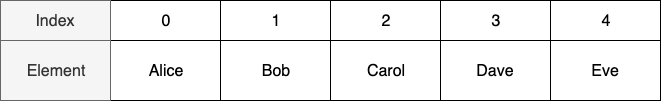
\includegraphics[width=\linewidth, keepratio]{chapters/07_python2_basics/figures/0-based-indexing.png}
                   \caption{Indizierung einer Liste mit 5 Elementen}
               \end{figure}
               
               Im Beispiel hat also das erste Element "Alice" den Index 0 und das letzte Element "Eve" den Index 4.
            \end{alertblock}
        \end{frame}
        
        \begin{frame}[fragile]{Speichern von Werten (VI)}
            \begin{itemize}
                \item \textbf{extend}: Einer Liste können auch Werte hinzugefügt werden, indem die Werte einer weiteren Liste angehängt werden. Hierzu kann die \code{extend()}-Funktion genutzt werden. Die Syntax ist: \\~\
                
                \code{<Liste>.extend(<Liste>)}
                
\begin{pyconcode}
>>> names = ['Alice', 'Bob' 'Carol']
>>> print(names)
['Alice', 'Bob', 'Carol']
>>> names.extend(['Dave', 'Eve'])
>>> print(names)
['Alice', 'Bob', 'Carol', 'Dave', 'Eve']
\end{pyconcode} 

            
            Mit \code{extend()} werden alle Elemente der zweiten Liste ans Ende der ersten Liste angehängt.
            \end{itemize}
        \end{frame}
        
        
        \begin{frame}[fragile]{Auslesen von Werten (I)}
            Um eine Liste sinnvoll nutzen zu können, ist es nicht nur wichtig, Werte in einer Liste abzuspeichern, sondern diese darüber hinaus auch wieder auslesen ("abfragen") zu können. \\~\
            
            Ebenso wie die Erzeugung einer Liste erfolgt die Abfrage eines Elements der Liste durch eckige Klammern, die den jeweiligen Index des gewünschten Elements einschließen. \\~\

\begin{pyconcode}
>>> names = ['Alice', 'Bob', 'Carol', 'Dave']
>>> second_name = names[1]
>>> print(second_name)
'Bob'
\end{pyconcode}             
        
            Hier wird das Element mit dem Index \texttt{1} aus der Liste \code{names} ausgelesen und in der Variablen \code{second\_name} gespeichert. Da die Indizierung 0-basiert ist, ist das Element mit dem Index \texttt{1} \textit{Bob} und nicht \textit{Alice}.
        \end{frame}
        
        \begin{frame}[fragile]{Auslesen von Werten (II)}
            \begin{alertblock}{Achtung}
                Der Programmierer muss stets darauf achten, einen validen Index anzugeben. Übersteigt der Index bspw. die Anzahl der in der Liste enthaltenen Elemente, erscheint ein Fehler

\begin{pyconcode}
>>> names = ['Alice', 'Bob', 'Carol', 'Dave']
>>> names[4]
IndexError: list index out of range
\end{pyconcode}  


            \end{alertblock}
        \end{frame}
        
        \begin{frame}[fragile]{Auslesen von Werten (III)}
            Die Abfrage von Werten mithilfe von Indizes kann auch mit negativen Indizes erfolgen. Hierdurch kann die Liste in umgekehrter Reihenfolge abgefragt werden. Dies macht beispielsweise das Auslesen des letzten Listenelements sehr bequem.

\begin{pyconcode}
>>> names = ['Alice', 'Bob', 'Carol', 'Dave']
>>> last_name = names[-1]
>>> print(last_name)
'Dave'
>>> names[1] == names[-3]
True
\end{pyconcode}  

        \begin{alertblock}{Achtung}
            Das letzte Listenelement besitzt den Index \texttt{-1} und nicht \texttt{-0}, da \texttt{-0} identisch zur Zahl \texttt{0} ist und daher schon für das erste Listenelement vergeben ist
        \end{alertblock}
        
        \end{frame}
        
        
        \begin{frame}[fragile]{Auslesen von Werten (IV)}
            Anstatt einzelner Elemente können auch Bereiche innerhalb einer Liste abgefragt werden. Hierfür wird das sogenannte \textbf{Slicing} genutzt. Die Syntax ist Ähnlich zur Abfrage einzelner Werte, jedoch wird hier ein Bereich von Indizes, getrennt durch \code{:} angegeben.
            
\begin{pyconcode}
>>> names = ['Alice', 'Bob', 'Carol', 'Dave', 'Eve']
>>> names[1:3]
['Bob', 'Carol']
>>> names[0:4]
['Alice', 'Bob', 'Carol', 'Dave']
\end{pyconcode}
        
        Die erste Zahl stellt dabei den Index dar, bei dem gestartet wird (inklusive), die zweite Zahl stellt den Endindex (exklusive) dar. Im 1. Beispiel wird also bei Index 1 ('Bob') begonnen und bei Index 3 ('Dave') gestoppt, da der Endindex jedoch exklusiv ist, werden lediglich Index 1 und 2 berücksichtigt.
        \end{frame}
        
        \begin{frame}[fragile]{Auslesen von Werten (IV)}
            Das Slicing kann noch um einen weiteren Wert, den \textbf{Step} erweitert werden. Indem neben Start und Stop ein dritter Wert angegeben wird, kann bestimmt werden, in welcher Schrittgröße die Elemente aus der Liste gelesen werden sollen. Wird kein Step angegeben (wie im vorherigen Beispiel), wird standardmäßig eine Schrittweite von 1 verwendet.
            
\begin{pyconcode}
>>> numbers = [0, 1, 2, 3, 4, 5, 6, 7]
>>> numbers[1:6:2]
[1, 3, 5]
\end{pyconcode}
        
        Es wird also der Bereich zwischen den Indizes 1 (inklusiv) und 6 (exklusiv) betrachtet und hiervon wird jede 2. Zahl berücksichtigt. Beginnend mit der 1 folgt dann die Zahl 3 sowie die Zahl 5. 
        
        \end{frame}
        
        \begin{frame}[fragile]{Auslesen von Werten (IV)}
            
            Wird kein Start-Index angegeben, wird automatisch bei Index 0 begonnen. Wird kein Stopindex angegeben, wird automatisch beim letzten Index gestoppt. Daher ist z.B. auch folgende Schreibweise denkbar:

 \begin{pyconcode}
>>> numbers = [0, 1, 2, 3, 4, 5, 6, 7]
>>> numbers[3:]
[3, 4, 5, 6, 7]
>>> numbers[:-2]
[0, 1, 2, 3, 4, 5]
>>> numbers[::2]
[0, 2, 4, 6]
\end{pyconcode}   
           Im ersten Beispiel werden alle Elemente beginnend beim 3. Index bis zum Ende der Liste (da kein Endindex angegeben ist) abgefragt (Schrittweite 1).
           
           Im zweiten Beispiel werden alle Elemente beginnend beim Anfang der Liste (da kein Startindex angegeben ist) bis zum vorvorletzten Element abgefragt (Schrittweite 1).
           
           Im dritten Beispiel werden alle Elemente beginnend beim Anfang der Liste (da kein Startindex angegeben ist) bis zum letzten Element (da kein Endindex angegeben ist) in 2-er Schritten abgefragt (\textit{jedes 2. Element der Liste})
          
        \end{frame}
        
         \begin{frame}[fragile]{Auslesen von Werten (IV)}
        
            Mithilfe von Slicing kann bspw. auch ganz einfach die Reihenfolge einer Liste umgekehrt werden:
 
 \begin{pyconcode}
>>> numbers = [0, 1, 2, 3, 4, 5, 6, 7]
>>> numbers[::-1]
[7, 6, 5, 4, 3, 2, 1, 0]
\end{pyconcode}         

        Hier wird vom Anfang der Liste bis zum Ende der Liste in Schritten der Größe \textit{-1}, also rückwärts, gegangen.
            
        \end{frame}
        
        \begin{frame}[fragile]{Löschen von Werten (I)}
            Neben der Möglichkeit, Werte zu einer Liste hinzuzufügen, können die Werte auch wieder gelöscht/entfernt werden, da Listen generell veränderbar sind. \\~\
            
            Auch hierfür stehen unterschiedliche Möglichkeiten zur Verfügung
        \end{frame}
        
        \begin{frame}[fragile]{Löschen von Werten (II)}
            \begin{itemize}
                \item \texttt{delete}-Operator: Um ein Element aus der Liste zu Löschen kann der \texttt{delete}-Operator genutzt werden. Hierfür steht das Schlüsselwort \code{del} zur Verfügung.  Die Syntax ist: \\~\
                
                \code{del <Liste>[<Index>]}
                
\begin{pyconcode}
>>> names = ['Alice', 'Bob', 'Carol', 'Dave']
>>> del names[0]
>>> print(names)
['Bob', 'Carol', 'Dave']
>>> del names[-1]
['Bob', 'Carol']
\end{pyconcode} 

            \end{itemize}
        \end{frame}
        
        
        \begin{frame}[fragile]{Löschen von Werten (III)}
            \begin{itemize}
                \item \textbf{pop}: Mithilfe der \code{pop()}-Funktion wird das Element entsprechend des übergebenen Indizes aus der Liste gelöscht und zurückgegeben. Wird kein Index explizit angegeben, wird das letzte Element der Liste gelöscht und zurückgegeben. Die Syntax ist: \\~\
                
                \code{<Liste>.pop()} bzw. \code{<Liste>.pop(<Index>)}
                
\begin{pyconcode}
>>> names = ['Alice', 'Bob', 'Carol', 'Dave']
>>> names.pop()
'Dave'
>>> print(names)
['Alice', 'Bob', 'Carol']
>>> names.pop(1)
Bob
>>> print(names)
['Alice', 'Carol']
\end{pyconcode} 

            \end{itemize}
        \end{frame}
        
        
        \begin{frame}[fragile]{Löschen von Werten (IV)}
            \begin{itemize}
                \item \textbf{remove}: Mithilfe der \code{remove()}-Funktion wird das erste Element aus der Liste gelöscht, das dem übergebenen Element entspricht. Ebenso wie bei der Abfrage von Werten muss stets darauf geachtet werden, ob der Wert überhaupt in der Liste enthalten ist, da ansonsten ein Fehler auftritt. Die Syntax ist: \\~\
                
                \code{<Liste>.remove(<Element>)}
                
\begin{pyconcode}
>>> names = ['Alice', 'Bob', 'Carol', 'Dave']
>>> names.remove('Bob')
>>> print(names)
['Alice', 'Carol', 'Dave']
>>> names.remove('Bob')
ValueError: list.remove(x): x not in list
\end{pyconcode} 

            \end{itemize}
        \end{frame}
        
        
        \begin{frame}[fragile]{in-Keyword}
            Um zu überprüfen, ob sich ein bestimmter Wert in einer Liste befindet (z.B. bevor die \code{remove()}-Funktion ausgeführt wird), gibt es in Python das Schlüsselwort \code{in}. 
            
            Die Auswertung ist dabei stets ein boolescher Wert: Falls das jeweilige Element in der Liste enthalten ist, wird \code{True} zurückgegeben, andernfalls \code{False}. 
            
            Die Syntax ist: \\~\
            
            \code{<Element> in <Liste>}
            
\begin{pyconcode}
>>> names = ['Alice', 'Bob', 'Carol', 'Dave']
>>> 'Bob' in names
True
>>> names.remove('Bob')
>>> print(names)
['Alice', 'Carol', 'Dave']
>>> 'Bob' in names
False
\end{pyconcode} 

        \end{frame}
        
        
        \begin{frame}[fragile]{Elementanzahl (I)}
            Um zu überprüfen, wie viele Elemente in einer Liste enthalten sind, kann die \code{len()}-Funktion genutzt werden. Diese gibt an, wie viele Werte insgesamt in der Liste gespeichert sind, es handelt sich also immer um einen Integer-Wert. 
            
            Die Syntax ist: \\~\
            
            \code{len(<Liste>)}
            
\begin{pyconcode}
>>> names = ['Alice', 'Bob', 'Carol', 'Dave']
>>> len(names)
4
>>> names.remove('Bob')
>>> print(names)
['Alice', 'Carol', 'Dave']
>>> len(names)
3
\end{pyconcode} 

        \end{frame}
        
        \begin{frame}[fragile]{Elementanzahl (II)}
            
            \begin{alertblock}{Achtung}
                Im Gegensatz zur mathematischen Zählweise bei der Indizierung wird bei der reinen Anzahl der Elemente die natürliche Zählweise genutzt. Wenn also in einer Liste 4 Elemente enthalten sind, ist die Anzahl der Elemente, die durch \code{len()} ermittelt wird, 4 und nicht 3. \\~\
                
                Dies führt in Kombination mit der Indizierung häufig zu Verwirrung und stellt eine häufige Fehlerursache dar.
            \end{alertblock}
        \end{frame}
        
        \begin{frame}[fragile]{Hilfreiche Funktionen (I)}
            
            Da Listen universell und flexibel einsetzbar sind, besitzen sie viele Hilfsfunktionen, die bereits in Python eingebaut sind und ohne weiteres vom Entwickler genutzt werden können. \\~\
            
            Eine Auswahl dieser Hilfsfunktionen wird im Folgenden vorgestellt, ein Überblick über alle Listenfunktionen gibt die \href{https://docs.python.org/3/tutorial/datastructures.html#more-on-lists}{offizielle Dokumentation}.
            
        \end{frame}
        
         \begin{frame}[fragile]{Hilfreiche Funktionen (II)}
            \begin{itemize}
                \item \textbf{sort}: Mithilfe der \code{sort()}-Funktion können Listen sortiert werden. 
                
                Die Syntax ist: \\~\
                
                \code{<Liste>.sort()} \\~\
                
                Sind in der Liste lediglich numerische Werte enthalten, so wird die Liste standardmäßig nach aufsteigende Werte sortiert:
                
\begin{pyconcode}
>>> numbers = [3, 6, 1, 9, 18, 4]
>>> numbers.sort()
>>> print(numbers)
[1, 3, 4, 6, 9, 18]
\end{pyconcode} 
            \end{itemize}
         \end{frame}
         
         \begin{frame}[fragile]{Hilfreiche Funktionen (III)}
            
            Sind in der Liste lediglich Strings enthalten, so wird die Liste standardmäßig alphabetisch aufsteigend sortiert:

\begin{pyconcode}
>>> addresses = ['Palm Springs 210', 'Sunset Blvd. 10', 'Eastriver Drive 50', '11th Street 09']
>>> addresses.sort()
>>> print(addresses)
['11th Street 09', 'Eastriver Drive 50', 'Palm Springs 210', 'Sunset Blvd. 10']
\end{pyconcode} 

             Sind in der Liste unterschiedliche Datentypen enthalten, so kann die Liste nicht sortiert werden, da unklar ist, wie etwa Strings und Integer-Werte miteinander verglichen werden sollen \footnote{In diesen Fällen kann der Entwickler eine eigene Vergleichs-/Sortierfunktion angeben}:

\begin{pyconcode}
>>> names_and_ages = ['Alice', 23, 'Bob', 21, 'Carol', 34, 'Dave', 19]
>>> names_and_ages.sort()
TypeError: '<' not supported between instances of 'int' and 'str'
\end{pyconcode} 

         \end{frame}
         
         
         \begin{frame}[fragile]{Hilfreiche Funktionen (IV)}
            
            Die Listen können auch absteigend sortiert werden, indem der Parameter \code{reverse=True} mit übergeben wird:
            
\begin{pyconcode}
>>> numbers = [3, 6, 1, 9, 18, 4]
>>> numbers.sort(reverse=True)
>>> print(numbers)
[18, 9, 6, 4, 3, 1]
\end{pyconcode} 

         \end{frame}
         
         
         \begin{frame}[fragile]{Hilfreiche Funktionen (V)}
            \begin{itemize}
                \item \textbf{reverse}: Analog zum Sortieren kann die Reihung der Elemente innerhalb einer Liste auch invertiert werden, die Liste wird also "umgedreht". Hierfür gibt es die \code{reverse()}-Funktion.
                
                Die Syntax ist: \\~\
                
                \code{<Liste>.reverse()}

\begin{pyconcode}
>>> names = ['Alice', 'Bob', 'Carol', 'Dave']
>>> names.reverse()
>>> print(names)
['Dave', 'Carol', 'Bob', 'Alice']
\end{pyconcode} 

            \end{itemize}
            
        \end{frame}
        
         \begin{frame}[fragile]{Hilfreiche Funktionen (VI)}
            \begin{itemize}
                \item \textbf{min/max/sum}: Auch mathematische Funktionen, die auf Listen angewandt werden können, sind vorhanden.
                
\begin{pyconcode}
>>> numbers = [3, 6, 1, 9, 18, 4]
>>> max(numbers)
18
>>> min(numbers)
1
>>> sum(numbers)
41
\end{pyconcode} 


            \end{itemize}
         \end{frame}
         
    
    \begin{subsubsection}{Aufgaben}
        \begin{frame}[allowframebreaks]{Aufgaben}
            \begin{enumerate}
                \item Was sind Listen? Wofür werden sie genutzt? Was ist der Vorteil ggü. zuvor besprochener Datentypen?
                \item Welche Eigenschaften besitzt eine Liste und was bedeuten diese?
                \item Wie können Listen erzeugt werden?
                \item Erzeugen Sie eine vorgefüllte Liste mit den Werten \texttt{1}, \texttt{3}, \texttt{5} und \texttt{7}
                \item Fügen sie dieser Liste den Wert \texttt{9} an
                \item Wie können mehrere Werte auf einmal angehängt werden? Fügen Sie die Werte \texttt{11}, \texttt{13} und \texttt{17} in einem Schritt an.
                \item Da der Wert \texttt{15} ausgelassen wurde, soll dieser nun ebenfalls zur Liste hinzugefügt werden, sodass die Sortierung der Werte intakt bleibt.
                \item Gegeben ist \code{x = [3,5,1,2,4,6]}. Welchen Wert hat \code{x[2]}? Welchen \code{x[-2]}?
                \item Mit welchem Befehl können in der zuvor erzeugten Liste der ungeraden Zahlen die Zahlen von 5 - 13 abgefragt werden?
                \item Wie kann diese Liste invertiert werden?
                \item Wie kann jeder dritte Wert dieser Liste abgefragt werden?
                \item Worin besteht der Unterschied zwischen \texttt{del}, \texttt{pop} und \texttt{remove}?
                \item Was ist das Ergebnis von \code{[1,1,2,2,3,3].remove(2)}?
                \item Wofür wird das \code{in}-Keyword genutzt? Was muss bei der Verwendung von Keywords beachtet werden?
                \item Worauf muss bei der Indizierung und der Längenangaben von Listen geachtet werden?
                \item Welche weitere Möglichkeit gibt es, die Reihenfolge einer Liste (permanent) umzukehren?
                \item Was ist das Ergebnis?: \code{max(['Bert', 'cArl', 'adam'])}
            \end{enumerate}
        \end{frame}
    \end{subsubsection}
    
    \begin{subsection}{Tuples}
    
        \begin{frame}{Tuples - Definition}
            Neben den Listen existiert ein weiterer häufig verbreiteter Sequenzdatentyp in Python: Das Tuple. Ein Tuple verhält sich sehr ähnlich zu einer Liste.
            
            \begin{block}{Tuple}
                Ein Tuple ist eine unveränderbare, geordnete und indizierte Sammlung von Objekten
            \end{block}
            
            Der primäre Unterschied zu Listen besteht also darin, dass Tuples unveränderbar sind, Werte können also nicht überschrieben und bestehende Tuples nicht abgeändert werden.
        \end{frame}
        
        \begin{frame}{Einsatz von Tuples}
            Ebenso wie Listen können auch in einem Tuple unterschiedliche Datentypen enthalten sein. \\~\
            
            Aufgrund der Unveränderbarkeit der Werte werden Tuples häufig als Rückgabewerte von Funktionen genutzt, sofern mehrere Werte zurückgegeben werden sollen.
        \end{frame}
        
        \begin{frame}[fragile]{Erzeugung (I)}
            Ein Tuple kann auf unterschiedliche Arten erzeugt werden: \\~\
            
            \begin{itemize}
                \item \code{tuple()}-Konstruktor: Mithilfe des Befehls \code{tuple()} kann ein neues, zunächst leeres Tuple erzeugt werden.
                
\begin{pyconcode}
>>> new_tuple = tuple()
>>> print(new_tuple)
()
>>> type(new_tuple)
<class 'tuple'>
\end{pyconcode}                 
            \end{itemize}
        \end{frame}
        
        \begin{frame}[fragile]{Erzeugung (II)}
            
            \begin{itemize}
                \item Kurzschreibweise: Elemente, die in einem Tuple enthalten sind, werden in Python durch runde Klammern (\code{( )}) umgeben. Als Kurzschreibweise kann anstatt \code{tuple()} daher auch einfach \code{()} genutzt werden.
                
\begin{pyconcode}
>>> new_tuple = ()
>>> print(new_tuple)
()
>>> type(new_tuple)
<class 'tuple'>
\end{pyconcode}                 
            \end{itemize}
        \end{frame}
        
        
        \begin{frame}[fragile]{Speichern von Werten (I)}
            
          In den beiden vorherigen Beispielen wurde gezeigt, wie Tuples erzeugt werden können, jedoch enthalten diese Tuples noch keine Werte, sind also \textit{leer}. Um Werte in den Tuples abzuspeichern gibt es die Möglichkeit, Werte direkt bei der Erzeugung anzugeben.
        \end{frame}
        
         \begin{frame}[fragile]{Speichern von Werten (II)}
         
         \begin{itemize}
             \item \textbf{Erzeugung eines vorgefüllten Tuples:} Bei der Initialisierung eines neuen Tuples können direkt Objekte angegeben werden, die in diesem Tuple gespeichert werden sollen: 

\begin{pyconcode}
>>> names = ('Alice', 'Bob', 'Carol', 'Dave')
>>> print(names)
('Alice', 'Bob', 'Carol', 'Dave')
>>> type(names)
<class 'tuple'>
\end{pyconcode}  
    
            Bei der Erzeugung von Tuples können die Klammern auch weggelassen werden. Jedoch sollten sie aus Gründen der Übersichtlichkeit immer genutzt werden.
            
\begin{pyconcode}
>>> names = 'Alice', 'Bob', 'Carol', 'Dave'
>>> type(names)
<class 'tuple'>
\end{pyconcode}  


         \end{itemize}
        \end{frame}
        
        \begin{frame}[fragile]{Speichern von Werten (III)}
            
            Soll ein Tuple mit lediglich einem Wert angelegt werden, ist das Komma trotzdem notwendig, um zwischen einer einfachen Wertzuweisung und einer Erzeugung eines Tuples unterscheiden zu können.
    
\begin{pyconcode}
>>> name_without_comma = ('Alice')
>>> name_with_comma = ('Alice',)
>>> type(name_without_comma)
<class 'str'>
>>> type(name_with_comma)
<class 'tuple'>
\end{pyconcode}  
        \end{frame}
        
        \begin{frame}[fragile]{Speichern von Werten (IV)}
         
            \begin{alertblock}{Achtung}
                Das gleichzeitige Erzeugen eines Tuples und Speichern von Werten in ebendiesem Tuple ist nur mit der Kurzschreibweise möglich. Wird ein Tuple mit tuple() erzeugt, können die Werte nicht direkt im Tuple gespeichert werden, auch ein späteres Hinzufügen ist nicht möglich (da Tuples unveränderbar sind).
            \end{alertblock}
        \end{frame}
        
        
        \begin{frame}[fragile]{Speichern von Werten (V)}
            \begin{alertblock}{Achtung}
               Funktionen wie \code{append()}, \code{insert()} oder \code{extend()} sind bei Tuples nicht vorhanden, da Tuples grundsätzlich unveränderbar sind.
            \end{alertblock}
        \end{frame}
      
        \begin{frame}[fragile]{Tuple-Operationen (I)}
           Es können verschiedene Operationen verwendet werden, um neue Tuple zu erzeugen: \\~\
           
           \begin{itemize}
               \item \textbf{Tuple Konkatenation}: Mithilfe des \code{+}-Operators können zwei Tuple konkateniert (verbunden) werden. Da die Tuple unveränderbar sind, entsteht dadurch ein neues, drittes Tuple

\begin{pyconcode}
>>> names1 = ('Alice', 'Bob')
>>> names2 = ('Carol', 'Dave')
>>> names3 = names1 + names2
>>> print(names3)
('Alice', 'Bob', 'Carol', 'Dave')
>>> type(names3)
<class 'tuple'>
\end{pyconcode}                 
               
           \end{itemize}
        \end{frame}
        
        
        \begin{frame}[fragile]{Tuple-Operationen (II)}

           \begin{itemize}
               \item \textbf{Multiple Konkatenation}: Mithilfe des \code{*}-Operators kann der Inhalt eines Tuples beliebig oft wiederholt werden. Da das Tuple unveränderbar ist, entsteht dadurch ein neues Tuple

\begin{pyconcode}
>>> names1 = ('Alice', 'Bob')
>>> names2 = names1 * 4
>>> print(names2)
('Alice', 'Bob', 'Alice', 'Bob', 'Alice', 'Bob', 'Alice', 'Bob')
>>> type(names2)
<class 'tuple'>
\end{pyconcode}                 
               
           \end{itemize}
        \end{frame}
        
        
        \begin{frame}[fragile]{Auslesen von Werten}
            Das Auslesen der Tuple-Werte verhält sich identisch zum Auslesen von Werten aus Listen. \\~\
            
            \begin{alertblock}{Achtung}
                Auch wenn Tuples mit runden Klammern erzeugt werden, erfolgt das Auslesen von Werten (wie bei allen Sequenz-Typen) mit eckigen Klammern!
            \end{alertblock}
            
            Auch Tuples sind indexbasiert, die wieder 0-basiert sind. Es muss auch beachtet werden, dass der Tuple-Index bei der Abfrage nicht größer ist als die Länge des Tuples
            
\begin{pyconcode}
>>> names = ('Alice', 'Bob', 'Carol', 'Dave')
>>> print(names[1])
'Bob'
>>> print(names[4])
IndexError: tuple index out of range
>>> print(names[-1])
'Dave'
\end{pyconcode}                 
               
                           
        \end{frame}
        
        
        \begin{frame}[fragile]{Löschen von Werten}
            Da Tuples unveränderlich sind, können Werte aus einem Tuple nicht entfernt werden. Wird trotzdem versucht, einen Wert zu löschen, erscheint ein Fehler:
            
\begin{pyconcode}
>>> names = ('Alice', 'Bob', 'Carol', 'Dave')
>>> del names[0]
TypeError: 'tuple' object doesn't support item deletion
\end{pyconcode}                 
        
        Soll trotzdem ein Wert aus einem Tuple gelöscht werden, kann dies über einen Workaround gelöst werden: Es kann ein neues Tuple, bestehend aus den Werten des alten Tuples exklusive des zu löschenden Wertes, erzeugt werden:

\begin{pyconcode}
>>> names = ('Alice', 'Bob', 'Carol', 'Dave')
>>> names_without_bob = (names[0],) + names[2:]
>>> print(names_without_bob)
('Alice', 'Carol', 'Dave')
\end{pyconcode}     
                           
        \end{frame}
        
        
         \begin{frame}[fragile]{in-Keyword}
            Ebenso wie bei den Listen kann mithilfe des \code{in}-Keywords festgestellt werden, ob ein Wert in einem Tuple enthalten ist.
            
\begin{pyconcode}
>>> names = ('Alice', 'Bob', 'Carol', 'Dave')
>>> 'Bob' in names
True
\end{pyconcode}                 
        
        \end{frame}
        
        
        \begin{frame}[fragile]{Elementzahl}
            Ebenso wie bei den Listen kann mithilfe der \code{len()}-Funktion festgestellt werden, wie viele Werte in einem Tuple enthalten sind.
            
\begin{pyconcode}
>>> names = ('Alice', 'Bob', 'Carol', 'Dave')
>>> len(names)
4
\end{pyconcode}                 
        
        \end{frame}
        
        
        \begin{frame}[fragile]{Hilfreiche Funktionen}
            Da Tuples unveränderbar sind, stehen hier keine der Funktionen zur Verfügung, die die Struktur der Tuples direkt verändern (z.B. \code{sort()}, \code{reverse()}, ...). \\~\
            
            Dennoch gibt es auch hier Tuple-Funktionen, die die Struktur nicht beeinflussen, wie etwa \code{min()}, \code{max()}, \code{sum()},...
            
\begin{pyconcode}
>>> ages = (23, 52, 21, 33)
>>> max(ages)
52
>>> sum(ages)
129
\end{pyconcode}                 
        
        \end{frame}
        
        
    
        \begin{subsubsection}{Aufgaben}
             \begin{frame}[allowframebreaks,fragile]{Aufgaben}
                \begin{enumerate}
                    \item Worin besteht der primäre Unterschied zwischen Listen und Tuples?
                    \item Wann werden Listen verwendet? Wann Tuples?
                    \item Welche Möglichkeiten gibt es, ein Tuple mit Werten zu füllen?
                    \item Welchen Zweck erfüllt der Tuple-Konstruktor?
                    \item Mit welchen der folgenden Ausdrücke wird ein Tuple erzeugt? Was ist jeweils das Ergebnis von \code{i[0]}?:
                        \begin{itemize}
                            \item
\begin{pyconcode}
>>> i = 0
>>> i[0]
\end{pyconcode}    
                            \item
\begin{pyconcode}
>>> i = (0)
>>> i[0]
\end{pyconcode}  
                            \item
\begin{pyconcode}
>>> i = (0),
>>> i[0]
\end{pyconcode}   
                            \item
\begin{pyconcode}
>>> i = (0,)
>>> i[0]
\end{pyconcode}   
                            \item
\begin{pyconcode}
>>> i = (0,),
>>> i[0]
\end{pyconcode}   
                            \item
\begin{pyconcode}
>>> i = 0,
>>> i[0]
\end{pyconcode}    
                            \item
\begin{pyconcode}
>>> i = "0"
>>> i[0]
\end{pyconcode}   
                           \item
\begin{pyconcode}
>>> i = "0,"
>>> i[0]
\end{pyconcode}   
                        \end{itemize}
                    \item Was ist bei Tuples bezüglich Kommas und Klammern zu beachten?
                    \item Wie kann dem Tuple \code{('Alice','Bob')} der Wert \code{'Carol'} angehängt werden?
                    \item Welche Ausgabe erzeugt folgender Befehl?:

\begin{pyconcode}
>>> tuple1 = ('na',)
>>> tuple2 = 'Batman',
>>> tuple1*10 + tuple2
\end{pyconcode}                     
                    \item Für den Zugriff auf Tuplewerte durch Indizes werden eckige Klammern verwendet. Warum werden diese nicht auch zur Erzeugung eines Tuples verwendet?
                    
                    \item Wie können Werte aus einem Tuple gelöscht werden? Was ist dabei zu beachten?
                    
                    \item Welche Funktionen sind bei Listen und Tuples anwendbar, welche lediglich bei Listen? Warum gilt diese Einschränkung?
                \end{enumerate}
            \end{frame}
        \end{subsubsection}
    \end{subsection}
    
    \begin{subsection}{Dictionaries}
    
        \begin{frame}{Dictionaries - Definition}
            Zu den erweiterten Grunddatentypen gehören bei Python auch die sogenannten \textit{Dictionaries}, die im deutschen auch seltener als \textit{Wörterbücher} bezeichnet werden.
            
            \begin{block}{Dictionary}
                Ein Dictionary ist eine veränderbare ungeordnete Sammlung von Werten in einer Key-Value Struktur
            \end{block}
        \end{frame}
    
        \begin{frame}{Key-Value Struktur}
            Eine \textit{Key-Value Struktur} ist eine in der Programmierung häufig genutzte Struktur, um eindeutige Relationen zwischen einem Schlüsselwert (\textbf{Key}) und einer entsprechenden Wertzuweisung (\textbf{Value}) herzustellen. \\~\
            
            \begin{exampleblock}{Beispiel}
                \textbf{Relation Länder \textrightarrow Hauptstädte:}
                
                \textit{"Deutschland"} \textrightarrow \textit{"Berlin"}, \textit{"Frankreich"} \textrightarrow \textit{"Paris"}, \textit{"Italien"} \textrightarrow \textit{"Rom"}, ... \\~\
                
                \textbf{Relation Name \textrightarrow Körpergröße:}
                
                \textit{"Alice"} \textrightarrow \textit{179}, \textit{"Bob"} \textrightarrow \textit{181}, \textit{"Eve"} \textrightarrow \textit{165}, ...\\~\
                
                \textbf{Relation Smarthome-Element \textrightarrow Zustand:}
                
                \textit{"Licht an"} \textrightarrow \textit{True}, \textit{"Fenster offen"} \textrightarrow \textit{False}, \textit{"Türe geschlossen"} \textrightarrow \textit{True}, ...
                

            \end{exampleblock}
        \end{frame}
        
        \begin{frame}{Eigenschaften}
            Ebenso wie Listen und im Gegensatz zu Tuples sind Dictionaries veränderbar, d.h. Werte innerhalb der Dictionaries können überschrieben und die Struktur der Dictionaries verändert werden, ohne dafür explizit ein neues Objekt erzeugen zu müssen. \\~\
            
            Im Gegensatz zu Listen und Tuples sind Dictionaries ungeordnet, d.h. die Elemente liegen nicht zwingend in der Reihenfolge vor, in der sie angelegt wurden. \footnote{Erst ab Python 3.7 sind Dictionaries immer \textit{insertion-ordered}}
            
            Da Dictionaries im Gegensatz zu den Sequence-Types nicht indexbasiert, sondern keybasiert ist, ist die Reihenfolge in den meisten Fällen irrelevant.
            
        \end{frame}
        
        \begin{frame}{Eigenschaften von Keys und Values}
            Die Keys und Values eines Dictionaries müssen gewisse Eigenschaften erfüllen:\\~\
            
            \begin{itemize}
                \item \textbf{Keys:}
                    \begin{itemize}
                        \item \textbf{Uniqueness:} Keys müssen \textit{unique} (eindeutig) sein. Es darf kein Wert mehrmals als Key innerhalb eines Dictionaries verwendet werden
                        \item \textbf{Hashable:} Keys müssen \textit{immutable} (unveränderbar) sein. Basisdatentypen (int, float, string, ...) sind also erlaubt, ebenso reine Tuples. Listen und Dictionaries sind veränderbar, daher können sie nicht als Key genutzt werden.
                        \item \textbf{Numerische Gleichheit:} Sofern zwei Zahlen als \textit{gleich} betrachtet werden, verweisen sie auf den selben Key (Bsp.: Da in Python gilt \code{1 == 1.0}, stellen beide Zahlen den gleichen Key dar)
                    \end{itemize}
                \item \textbf{Values:}
                    \begin{itemize}
                        \item Annähernd alle Objekte und Datentypen dürfen als Values innerhalb eines Dictionaries verwendet werden, z.B. Grunddatentypen (int, float, string, ...), erweiterte Datentypen (Sequenzen (Listen, Tuples), Maps (Dictionaries), Sets), Klassen, Objekte, ...
                    \end{itemize}
            \end{itemize}
        \end{frame}
        
        \begin{frame}[fragile]{Erzeugung (I)}
            Ein Dictionary kann auf unterschiedliche Arten erzeugt werden:
            
            \begin{itemize}
                \item \code{dict()}-Konstruktor: Mithilfe des Befehls \code{dict()} kann ein neues, zunächst \textit{leeres} Dictionary erzeugt werden
            \end{itemize}

\begin{pyconcode}
>>> new_dictionary = dict()
>>> print(new_dictionary)
{}
>>> type(new_dictionary)
<class 'dict'>
\end{pyconcode}             
    
        \end{frame}
        
        \begin{frame}[fragile]{Erzeugung (II)}
            
            \begin{itemize}
                \item Kurzschreibweise: Elemente, die in einem Dictionary enthalten sind, werden in Python durch geschweifte Klammern (\code{\{ \}}) umgeben. Als Kurzschreibweise kann anstatt \code{dict()} daher auch einfach \code{\{\}} genutzt werden
            \end{itemize}

\begin{pyconcode}
>>> new_dictionary = {}
>>> print(new_dictionary)
{}
>>> type(new_dictionary)
<class 'dict'>
\end{pyconcode}             
    
        \end{frame}

        
        \begin{frame}[fragile]{Speichern von Werten (I)}
            
            In beiden vorherigen Beispielen wurde gezeigt, wie Dictionaries erzeugt werden können, jedoch enthalten diese Dictionaries noch keine Werte, sind also \textit{leer}. Um Werte in den Listen abzuspeichern, gibt es unterschiedliche Möglichkeiten.
    
        \end{frame}
    
        \begin{frame}[fragile]{Speichern von Werten (II)}
            
           \begin{itemize}
               \item \textbf{Erzeugung eines vorgefüllten Dictionaries:} Bei der Initialisierung eines neuen Dictionaries können direkt Objekte angegeben werden, die in diesem Dictionary gespeichert werden sollen:

\begin{pyconcode}
>>> capitals = {'Germany': 'Berlin', 'France': 'Paris', 'Italy': 'Rome'}
>>> print(capitals)
{'Germany': 'Berlin', 'France': 'Paris', 'Italy': 'Rome'}
>>> type(capitals)
<class 'dict'>
\end{pyconcode}

            Hier wird ein Dictionary erzeugt, das jeweils einem Land (Key) eine Hauptstadt (Value) zuweist. Die Syntax eines Dictionaries sieht folgendermaßen aus: \\~\
            
            \code{\{<Key>: <Value>, <Key>: <Value>, ...\}}
            
            Einzelne Einträge werden also durch Komma getrennt, Values werden den Keys durch Doppelpunkt zugewiesen.

           \end{itemize}
    
        \end{frame}
        
        \begin{frame}[fragile]{Speichern von Werten (III)}
            
          \begin{alertblock}{Achtung}
            Das gleichzeitige Erzeugen eines Dictionaries und Speichern von Werten in ebendiesem Dictionary ist nur mit Kurzschreibweise möglich. Wird ein Dictionary mit \code{dict()} erzeugt, können die Werte nicht direkt im Dictionary gespeichert werden, hierzu ist ein extra Schritt notwendig.
          \end{alertblock}
    
        \end{frame}
        
        
         \begin{frame}[fragile]{Speichern von Werten (IV)}
            
            \begin{itemize}
                \item \textbf{insert:} Anders als bei den Listen gibt es keine dedizierten \code{append()}, \code{insert()}, ... Funktionen, sondern um einen Wert im Dictionary zu ergänzen bzw. zu überschreiben, genügt folgender Wertzuweisung:\\~\
                
                \code{<Dictionary>[<Key>] = <Value>}
                
                Dies entspricht der normalen Wertzuweisung von Variablen.
            
\begin{pyconcode}
>>> capitals = {'Germany': 'Berlin', 'France': 'Paris', 'Italy': 'Rome'}
>>> print(capitals)
{'Germany': 'Berlin', 'France': 'Paris', 'Italy': 'Rome'}
>>> capitals['Spain'] = 'Barcelona'
>>> print(capitals)
{'Germany': 'Berlin', 'France': 'Paris', 'Italy': 'Rome', 'Spain': 'Barcelona'}
>>> capitals['Spain'] = 'Madrid'
>>> print(capitals)
{'Germany': 'Berlin', 'France': 'Paris', 'Italy': 'Rome', 'Spain': 'Madrid'}
\end{pyconcode}    
                
            \end{itemize}
    
        \end{frame}
        
        \begin{frame}[fragile]{Speichern von Werten (V)}
            
            \begin{itemize}
                \item \textbf{update:} Darüber hinaus existiert auch die \code{update()}-Methode, um Werte dem Dictionary hinzuzufügen bzw. bestehende Werte zu aktualisieren. Die Syntax ist:\\~\
                
                \code{<Dictionary>.update(<Dictionary>)}
                
                Falls das jeweilige Key-Value-Paar im Dictionary bereits vorhanden ist, wird es überschrieben, andernfalls wird es ergänzt.
            
\begin{pyconcode}
>>> capitals = {'Germany': 'Berlin', 'France': 'Paris', 'Italy': 'Rome', 'Spain': 'Barcelona'}
>>> print(capitals)
{'Germany': 'Berlin', 'France': 'Paris', 'Italy': 'Rome', 'Spain': 'Barcelona'}
>>> capitals.update({'Spain':'Madrid', 'Austria': 'Vienna'})
>>> print(capitals)
{'Germany': 'Berlin', 'France': 'Paris', 'Italy': 'Rome', 'Spain': 'Madrid', 'Austria': 'Vienna'}
\end{pyconcode}    
                
            \end{itemize}
    
        \end{frame}
        
        
        \begin{frame}[fragile]{Auslesen von Werten (I)}
            
            Ebenso wie bei Listen und Tuples können Werte aus den Dictionaries mit eckigen Klammern abgefragt werden. Jedoch sind Dictionaries nicht indexbasiert, sondern keybasiert. D.h. auf die jeweiligen Werte kann durch den zugehörigen Key zugegriffen werden.
            
\begin{pyconcode}
>>> capitals = {'Germany': 'Berlin', 'France': 'Paris', 'Italy': 'Rome'}
>>> print(capitals['Germany'])
'Berlin'
\end{pyconcode}    
                
    
        \end{frame}
    
        \begin{frame}[fragile]{Auslesen von Werten (II)}
            
            \begin{alertblock}{Achtung}
                Der Programmierer muss stets darauf achten, einen validen Key anzugeben. Ist der jeweilige Key nicht im Dictionary enthalten, erscheint ein Fehler
                
\begin{pyconcode}
>>> capitals = {'Germany': 'Berlin', 'France': 'Paris', 'Italy': 'Rome'}
>>> print(capitals['Norway'])
KeyError: 'Norway'
\end{pyconcode}    
    
        \end{alertblock}
    
        \end{frame}
        
        \begin{frame}[fragile]{Auslesen von Werten (III)}
            
            \begin{alertblock}{Achtung}
                Im Dictionary können Wert lediglich anhand des Keys abgefragt werden. Eine Abfrage nach Wert ist nicht möglich (Analogie: Wörterbuch)
            
\begin{pyconcode}
>>> capitals = {'Germany': 'Berlin', 'France': 'Paris', 'Italy': 'Rome'}
>>> print(capitals['Berlin'])
KeyError: 'Berlin'
\end{pyconcode}    
                
        \end{alertblock}
        \end{frame}
        
        \begin{frame}[fragile]{Auslesen von Werten (IV)}
            
            Dem Programmierer steht darüber hinaus die \code{get()}-Methode zur Verfügung. Ebenso wie bei der zuvor gezeigten key-basierten Abfrage mithilfe eckiger Klammern können so die Werte zu einem Key abgefragt werden. Außerdem kann ein Default-Wert angegeben werden, der als Ergebnis zurückgegeben wird, falls der Key nicht vorhanden ist.
            
\begin{pyconcode}
>>> capitals = {'Germany': 'Berlin', 'France': 'Paris', 'Italy': 'Rome'}
>>> capital = capitals.get('France')
>>> print(capital)
'Paris'
>>> capital = capitals.get('Norway')
>>> print(capital)
None
>>> capital = capitals.get('Norway', 'nicht enthalten')
>>> print(capital)
'nicht enthalten'
\end{pyconcode}    
                
        
        \end{frame}
    
        \begin{frame}[fragile]{Löschen von Werten (I)}
            
           Neben der Möglichkeit, Werte zu einem Dictionary hinzuzufügen, können die Werte auch wieder gelöscht/entfernt werden, da Dictionaries generell veränderbar sind. \\~\
           
           Auch hierfür stehen unterschiedliche Möglichkeiten zur Verfügung
                
        \end{frame}
        
        \begin{frame}[fragile]{Löschen von Werten (II)}
        
            \begin{itemize}
                \item \texttt{delete}-Operator: Um ein Element aus der Liste zu löschen kann der \texttt{delete}-Operator genutzt werden. Hierfür steht das Schlüsselwort \code{del} zur Verfügung. Die Syntax ist: \\~\
                
                \code{del <Dictionary>[<Key>]}
                
\begin{pyconcode}
>>> capitals = {'Germany': 'Berlin', 'France': 'Paris', 'Italy': 'Rome'}
>>> print(capitals)
{'Germany': 'Berlin', 'France': 'Paris', 'Italy': 'Rome'}
>>> del capitals['Germany']
>>> print(capitals)
{'France': 'Paris', 'Italy': 'Rome'}
\end{pyconcode}  
            \end{itemize}
                
        \end{frame}
        
        \begin{frame}[fragile]{Löschen von Werten (III)}
        
            \begin{itemize}
                \item \textbf{pop}: Mithilfe der \code{pop()}-Methode wird ein Key-Value-Paar anhand des Key-Wertes aus dem Dictionary gelöscht. Zudem wird der Wert des gelöschten Paares zurückgegeben. Die Syntax ist: \\~\
                
                \code{<Dictionary>.pop(<Key>)}
                
\begin{pyconcode}
>>> capitals = {'Germany': 'Berlin', 'France': 'Paris', 'Italy': 'Rome'}
>>> print(capitals)
{'Germany': 'Berlin', 'France': 'Paris', 'Italy': 'Rome'}
>>> removed_capital = capitals.pop('France')
>>> print(removed_capital)
'Paris'
\end{pyconcode}  
            \end{itemize}
                
        \end{frame}
        
        \begin{frame}[fragile]{Löschen von Werten (IV)}
        
            \begin{itemize}
                \item \textbf{popitem}: Mithilfe der \code{popitem()}-Methode wird ein zufälliges Key-Value-Paar aus dem Dictionary gelöscht. Zudem wird das Key-Value-Paar des gelöschten Elements als Tuple zurückgegeben. Die Syntax ist: \\~\
                
                \code{<Dictionary>.popitem()}
                
\begin{pyconcode}
>>> capitals = {'Germany': 'Berlin', 'France': 'Paris', 'Italy': 'Rome'}
>>> print(capitals)
{'Germany': 'Berlin', 'France': 'Paris', 'Italy': 'Rome'}
>>> removed_capital = capitals.popitem()
>>> print(removed_capital)
('Italy', 'Rome')
\end{pyconcode}  
            \end{itemize}
                
        \end{frame}
        
        \begin{frame}[fragile]{Löschen von Werten (V)}
        
            \begin{itemize}
                \item \textbf{clear}: Mithilfe der \code{clear()}-Methode werden alle Key-Value-Paare aus dem Dictionary gelöscht. Die Syntax ist: \\~\
                
                \code{<Dictionary>.clear()}
                
\begin{pyconcode}
>>> capitals = {'Germany': 'Berlin', 'France': 'Paris', 'Italy': 'Rome'}
>>> print(capitals)
{'Germany': 'Berlin', 'France': 'Paris', 'Italy': 'Rome'}
>>> capitals.clear()
>>> print(capitals)
{}
\end{pyconcode}  
            \end{itemize}
                
        \end{frame}
        
        \begin{frame}[fragile]{in-Keyword}
        
            Ebenso wie bei Listen und Tuples, kann das \code{in}-Keyword genutzt werden, um zu überprüfen, ob sich ein Key in einem Dictionary befindet.
                
\begin{pyconcode}
>>> capitals = {'Germany': 'Berlin', 'France': 'Paris', 'Italy': 'Rome'}
>>> 'Italy' in capitals
True
>>> 'Berlin' in capitals
False
\end{pyconcode}  
        
                
        \end{frame}
        
        \begin{frame}[fragile]{Elementanzahl}
        
            Um zu überprüfen, wie viele Key-Value-Paare sich in einem Dictionary befinden, kann die \code{len()}-Funktion genutzt werden.
                
\begin{pyconcode}
>>> capitals = {'Germany': 'Berlin', 'France': 'Paris', 'Italy': 'Rome'}
>>> len(capitals)
3
>>> capitals.clear()
0
\end{pyconcode}  
        
                
        \end{frame}
        
        \begin{frame}[fragile]{Hilfreiche Funktionen (I)}
        
            Da Dictionaries universell und flexibel einsetzbar sind, besitzen sie viele Hilfsfunktionen, die bereits in Python eingebaut sind und ohne weiteres vom Entwickler genutzt werden können.\\~\
            
            Eine Auswahl dieser Hilfsfunktionen wird im Folgenden vorgestellt, ein Überblick über alle Dictionaryfunktionen gibt die \href{https://docs.python.org/3/tutorial/datastructures.html#dictionaries}{offizielle Dokumentation}
                
        \end{frame}
        
        \begin{frame}[fragile]{Hilfreiche Funktionen (II)}
        
            \begin{itemize}
                \item \textbf{items:} Mithilfe der \code{items()}-Methode werden alle Key-Value-Paare in einem sogenannten \textit{View-Objekt}\footnote{View-Objekte stellen eine dynamische Repräsentation der Dictionaries dar. Sie können wie Listen verwendet werden} zurückgegeben. Jedes Key-Value-Paar wird durch ein Tuple repräsentiert. Die Syntax ist: \\~\
                
                \code{<Dictionary>.items()}
  
\begin{pyconcode}
>>> capitals = {'Germany': 'Berlin', 'France': 'Paris', 'Italy': 'Rome'}
>>> items = capitals.items()
>>> print(items)
dict_items([('Germany', 'Berlin'), ('France', 'Paris'), ('Italy', 'Rome')])
\end{pyconcode}                
                
            \end{itemize}
                
        \end{frame}
        
        \begin{frame}[fragile]{Hilfreiche Funktionen (III)}
        
            \begin{itemize}
                \item \textbf{keys:} Mithilfe der \code{keys()}-Methode werden alle Keys des Dictionaries in einem \textit{View-Objekt} zurückgegeben. Die Syntax ist: \\~\
                
                \code{<Dictionary>.keys()}
  
\begin{pyconcode}
>>> capitals = {'Germany': 'Berlin', 'France': 'Paris', 'Italy': 'Rome'}
>>> keys = capitals.keys()
>>> print(keys)
dict_keys(['Germany', 'France', 'Italy'])
\end{pyconcode}                
                
            \end{itemize}
                
        \end{frame}
        
        \begin{frame}[fragile]{Hilfreiche Funktionen (IV)}
        
            \begin{itemize}
                \item \textbf{values:} Mithilfe der \code{values()}-Methode werden alle Values des Dictionaries in einem \textit{View-Objekt} zurückgegeben. Die Syntax ist: \\~\
                
                \code{<Dictionary>.values()}
  
\begin{pyconcode}
>>> capitals = {'Germany': 'Berlin', 'France': 'Paris', 'Italy': 'Rome'}
>>> values = capitals.values()
>>> print(values)
dict_values(['Berlin', 'Paris', 'Rome'])
\end{pyconcode}                
                
            \end{itemize}
                
        \end{frame}
        
        \begin{frame}[fragile]{Hilfreiche Funktionen (V)}
        
             Auf Dictionaries (bzw. deren Werte) können auch Mengenoperationen durchgeführt werden. Die folgenden Beispiele sind jeweils für die \code{items()}-Methode anwendbar. \\~\
            
            \begin{itemize}
                \item \textbf{Schnittmenge:} Mithilfe des \code{\&}-Operators können Schnittmengen zwischen Dictionaries erstellt werden. Das Ergebnis der Schnittmengen-Operation sind diejenigen Elemente, die in beiden Dictionaries vorhanden sind (\textbf{AND}-Verknüpfung).
  

\begin{pyconcode}
>>> capitals1 = {'Germany': 'Berlin', 'France': 'Paris', 'Italy': 'Rome'}
>>> capitals2 = {'Germany': 'Berlin', 'Spain': 'Madrid'}
>>> intersection =  capitals1.items() & capitals2.items()
>>> print(intersection)
{('Germany', 'Berlin')}
\end{pyconcode}                
            
            \end{itemize}
                
        \end{frame}
        
        \begin{frame}[fragile]{Hilfreiche Funktionen (VI)}
                
                \begin{itemize}
                    \item \textbf{Vereinigung:} Mithilfe des \code{|}-Operators können Mengen-Vereinigungen erstellt werden. Das Ergebnis der Vereinigungs-Operation sind diejenigen Elemente, die in mindestens einem der beiden Dictionaries vorhanden sind (\textbf{OR}-Verknüpfung).
      
  
\begin{pyconcode}
>>> capitals1 = {'Germany': 'Berlin', 'France': 'Paris', 'Italy': 'Rome'}
>>> capitals2 = {'Germany': 'Berlin', 'Spain': 'Madrid'}
>>> union =  capitals1.items() | capitals2.items()
>>> print(union)
{('Spain', 'Madrid'), ('Italy', 'Rome'), ('Germany', 'Berlin'), ('France', 'Paris')}
\end{pyconcode}                
                
          \end{itemize}
                
        \end{frame}
        
        \begin{frame}[fragile]{Hilfreiche Funktionen (VII)}
                
                \begin{itemize}
                    \item \textbf{Symmetrische Differenz:} Mithilfe des \code{\^}-Operators können symmetrische Differenzen erstellt werden. Das Ergebnis der Operation sind diejenigen Elemente, die in genau einem der beiden Dictionaries vorhanden sind, aber nicht in beiden (\textbf{XOR}-Verknüpfung).
      
  
\begin{pyconcode}
>>> capitals1 = {'Germany': 'Berlin', 'France': 'Paris', 'Italy': 'Rome'}
>>> capitals2 = {'Germany': 'Berlin', 'Spain': 'Madrid'}
>>> symm_diff =  capitals1.items() ^ capitals2.items()
>>> print(symm_diff)
{('Spain', 'Madrid'), ('Italy', 'Rome'), ('France', 'Paris')}
\end{pyconcode}                
                
          \end{itemize}{}
                
        \end{frame}
        
                \begin{frame}[fragile]{Hilfreiche Funktionen (VIII)}
                
                \begin{itemize}
                    \item \textbf{Differenz:} Mithilfe des \code{-}-Operators können Differenzen erstellt werden. Das Ergebnis der Differenz-Operation sind diejenigen Elemente, die im ersten Dictionary, nicht aber im zweiten Dictionary enthalten sind (\textbf{not}-Operation).
      
  
\begin{pyconcode}
>>> capitals1 = {'Germany': 'Berlin', 'France': 'Paris', 'Italy': 'Rome'}
>>> capitals2 = {'Germany': 'Berlin', 'Spain': 'Madrid'}
>>> diff =  capitals1.items() - capitals2.items()
>>> print(diff)
{('Italy', 'Rome'), ('France', 'Paris')}
\end{pyconcode}                
                
          \end{itemize}
                
        \end{frame}
        
        \begin{subsubsection}{Aufgaben}
             \begin{frame}[allowframebreaks,fragile]{Aufgaben}
                \begin{enumerate}
                    \item Welcher Analogie folgen die Dictionaries in Python bzw. allgemein Key-Value-Stores in der Programmierung?
                    \item Worin unterscheiden sich Dictionaries von Listen bzw. Tuples? Was sind die Gemeinsamkeiten?
                    \item Was wird durch eine Key-Value-Struktur repräsentiert?
                    \item In welchen anderen Bereichen der bereits besprochenen Themengebiete treten Key-Value-Strukturen auf?
                    \item Warum sind Dictionaries nicht zwingend geordnet?
                    \item Welche Eigenschaften müssen die Keys eines Dictionaries erfüllen? Welche die Values? Warum sind die Regeln der Values nicht so strikt?
                    \item Folgendes Snippet ist gegeben:

\begin{pyconcode}
>>> x = {3.0: 'Alice'}
>>> x['Alice'] = 3.0
>>> x['Bob'] = 3
>>> x[3] = 'Bob'
\end{pyconcode} 
                Welchen Wert besitzt \code{x}?
                    \item Welche Unterschiede bestehen zwischen dem \code{dict()}-Konstruktor und der Kurzschreibweise \code{[]} zum Erzeugen eines Dictionaries?
                    
                    \item Warum gibt es im Gegensatz zur Liste, die ebenfalls veränderbar ist, keine Basisfunktion wie \code{append()} zum Hinzufügen neuer Werte zum Dictionary?
                    
                    \item Welchen Vorteil bietet die \code{update()}-Methode gegenüber der normalen Wertzuweisung?
                    
                    \item Was passiert, wenn mit \code{update()} ein Key-Value-Paar aktualisiert werden soll, das im Dictionary nicht existiert?
                    
                    \item Was passiert, wenn Key-Value-Paare anhand ihres Values ausgelesen werden?
                    
                    \item Kann bei Dictionaries ebenso wie bei Listen und Tuples per negativen Index zugegriffen werden? Ist Slicing möglich?`
                    
                    \item Welche Möglichkeiten gibt es, einen Wert aus dem Dictionary auszulesen, wobei der Entwickler nicht sicher ist, ob der jeweilige Key existiert?
                    
                    \item Wird mit dem \code{del}-Keyword lediglich der entsprechende Wert anhand des Schlüssels aus dem Dictionary gelöscht oder der komplette Key-Value-Paar?
                    
                    \item Nach welcher Logik werden mit \code{popitem()} Elemente aus dem Dictionary entfernt? Wozu könnte diese Funktion hilfreich sein?
                    
                    \item Bezieht sich das \code{in}-Keyword auf Keys oder Values?
                    
                    \item Auf was bezieht sich \code{len()}-Funktion?
                    
                    \item Wie kann eine Liste mit allen Values eines Dictionaries ausgegeben werden?
                    
                    \item Auf welche boolesche Operationen beziehen sich die Schnittmenge, Vereinigung, symmetrische Differenz und Differenz von Dictionaries? Warum werden diese nicht durch die zuvor besprochenen Keywords ausgedrückt?

                \end{enumerate}
            \end{frame}
        \end{subsubsection}
    \end{subsection}
    
    \begin{subsection}{Sets}
    
        \begin{frame}{Sets - Definition}
            Sets verhalten sich sehr ähnlich zu Listen und Tuples. Der primäre Unterschied besteht in der Eigenschaft, dass Sets keine identischen Werte enthalten können.
            
            \begin{block}{Set}
                Ein Set ist eine \textit{veränderbare} und \textit{ungeordnete} Sammlung von \textit{unterschiedlichen} (\textit{"unique"}) Objekten.
            \end{block}
        \end{frame}
        
        \begin{frame}{Einsatz von Sets}
            Sets werden i.d.R. analog zu Listen verwendet, können jedoch eine Zeitersparnis darstellen bzw. eine Einhaltung der Eindeutigkeitslogik erzwingen, indem der Entwickler nicht selbst überprüfen muss, ob sich ein Element bereits in der Liste befindet, da die Eindeutigkeit durch Sets garantiert wird.
            
        \end{frame}
        
        \begin{frame}[fragile]{Erzeugung von Sets (I)}
            Auch Sets können auf unterschiedliche Arten erzeugt werden:
            
            \begin{itemize}
                \item \code{set()}-Konstruktor: Mithilfe des \code{set()}-Konstruktors kann ein neues Set-Objekt erzeugt werden
                
\begin{pyconcode}
>>> new_set = set()
>>> print(new_set)
set()
>>> type(new_set)
<class 'set'>
\end{pyconcode} 

            \end{itemize}
            
        \end{frame}
        
        
        \begin{frame}[fragile]{Erzeugung von Sets (II)}
     
            \begin{itemize}
                \item Kurzschreibweise: Als Kurzschreibweise können anstatt \code{set()} auch einfach geschweifte Klammern (\code{\{ \}}) genutzt werden
                
\begin{pyconcode}
>>> new_set = {'Alice', 'Bob', 'Carol', 'Alice'}
>>> print(new_set)
{'Alice', 'Carol', 'Bob'}
>>> type(new_set)
<class 'set'>
\end{pyconcode} 
            
                \begin{alertblock}{Achtung}
                    Für Sets werden ebenso wie für Dictionaries geschweifte Klammern genutzt. Falls es sich um eine reine Aneinanderreihung von Einzelwerten handelt, wird ein Set erzeugt. Werden Key-Value-Paare übergeben, wird ein Dictionary erzeugt. Da der Befehl \code{\{ \}} schon zur Erzeugung eines leeren Dictionaries verwendet wird, kann damit kein leeres Set erzeugt werden. Lediglich ein vorgefülltes Set kann mit der Kurzschreibweise erzeugt werden.
                \end{alertblock}

            \end{itemize}
            
        \end{frame}
        
        \begin{frame}[fragile]{Speichern von Werten (I)}
     
            \begin{itemize}
                \item \textbf{add}: Um einen (hashbaren) Wert der Liste hinzuzufügen, kann die \code{add()}-Methode genutzt werden. Der übergebene Wert wird nur dann hinzugefügt, falls er noch nicht in der Liste vorhanden ist. Die Syntax ist: \\~\
                
                \code{<Set>.add(<Element>)}
                
\begin{pyconcode}
>>> new_set = {'Alice', 'Bob', 'Carol', 'Alice'}
>>> print(new_set)
{'Alice', 'Carol', 'Bob'}
>>> new_set.add('Dave')
>>> print(new_set)
{'Alice', 'Dave', 'Carol', 'Bob'}
>>> new_set.add('Dave')
{'Alice', 'Dave', 'Carol', 'Bob'}
\end{pyconcode} 
            
            \end{itemize}
            
        \end{frame}
        
        \begin{frame}[fragile]{Speichern von Werten (I)}
            \begin{itemize}
                    \item \textbf{update}: Um mehrere (nicht-hashbare) Werte der Liste hinzuzufügen, kann die \code{update()}-Methode genutzt werden. Die übergebenen Werte werden nur dann hinzugefügt, falls sie noch nicht in der Liste vorhanden sind. Die Syntax ist: \\~\
                    
                    \code{<Set>.update(<Elements>)}
                    
\begin{pyconcode}
>>> new_set = {'Alice', 'Bob', 'Carol', 'Alice'}
>>> print(new_set)
{'Alice', 'Carol', 'Bob'}
>>> new_set.update({'Dave'})
>>> print(new_set)
{'Carol', 'Alice', 'Bob', 'Dave'}
\end{pyconcode} 
            
                \end{itemize}
            
        \end{frame}
        
        \begin{frame}[fragile]{Speichern von Werten (I)}
            
            \begin{alertblock}{Achtung}
                Um einen einzelnen Wert zum Set hinzuzufügen, wird die \code{add()}-Methode genutzt. Ein Hinzufügen von mehreren Werten gleichzeitig ist damit nicht möglich, solange sie nicht-hashable (\textit{veränderbar}) sind, z.B. Listen und Sets. Ein Hinzufügen von einem Tuple dagegen ist möglich (da unveränderbar).
                
                Sollen mehrere Werte, die nicht-hashable sind, hinzugefügt werden, muss \code{update()} verwendet werden. Diese Methode akzeptiert eine unbegrenzte Anzahl von \textit{Argumenten}. Dafür können hiermit keine "Einzelwerte" (nicht-iterierbar) hinzugefügt werden.
                
\begin{pyconcode}
>>> new_set = {'Alice', 'Bob'}
>>> new_set.add('Carol')
>>> print(new_set)
{'Carol', 'Alice', 'Bob'}
>>> new_set.add(['Dave', 'Eve'])
TypeError: unhashable type: 'list'
>>> new_set.update(['Dave', 'Eve'])
>>> print(new_set)
{'Eve', 'Dave', 'Carol', 'Alice', 'Bob'}
>>> new_set.update(5)
TypeError: 'int' object is not iterable
\end{pyconcode} 
            \end{alertblock}
        \end{frame}
        
        \begin{frame}[fragile]{Auslesen von Werten (I)}
            Da Sets weder index- noch keybasiert sind und darüber hinaus keine feste Ordnung besitzen, gibt es keine Abfrage von Werten, die mit dem Auslesen von Listen, Tuples oder Dictionaries vergleichbar ist. \\~\
            
            Da aber eine reine Speicherung von Werten ohne der Möglichkeit, den Inhalt der Werte auslesen zu können, sinnlos ist, gibt es dennoch Wege, an die entsprechenden Werte zu gelangen. \\~\
            
            Dies ist beispielsweise möglich, indem durch das Set \textit{iteriert} wird. \footnote{Diese Funktionalität bezieht sich auf \textit{Schleifen}, die im nächsten Foliensatz besprochen wird}
        \end{frame}
        
        \begin{frame}[fragile]{Löschen von Werten (I)}
            \begin{itemize}
                \item \textbf{discard}: Mit der \code{discard()}-Methode kann ein bestimmtes Element aus dem Set entfernt werden. Existiert der entsprechende Wert nicht im Set, wird der Aufruf ignoriert. 
                
                Die Syntax ist: \\~\
                
                \code{<Set>.discard(<Element>)}
                
\begin{pyconcode}
>>> new_set = {'Alice', 'Bob', 'Carol'}
>>> print(new_set)
{'Carol', 'Alice', 'Bob'}
>>> new_set.discard('Bob')
>>> print(new_set)
{'Carol', 'Alice'}
>>> new_set.discard('Eve')
>>> print(new_set)
{'Carol', 'Alice'}
\end{pyconcode} 

            \end{itemize}
        \end{frame}
        
        
        \begin{frame}[fragile]{Löschen von Werten (II)}
            \begin{itemize}
                \item \textbf{remove}: Mit der \code{remove()}-Methode kann ein bestimmtes Element aus dem Set entfernt werden. Existiert der entsprechende Wert nicht im Set, wird ein Fehler geworfen. 
                
                Die Syntax ist: \\~\
                
                \code{<Set>.remove(<Element>)}
                
\begin{pyconcode}
>>> new_set = {'Alice', 'Bob', 'Carol'}
>>> print(new_set)
{'Carol', 'Alice', 'Bob'}
>>> new_set.remove('Bob')
>>> print(new_set)
{'Carol', 'Alice'}
>>> new_set.remove('Eve')
KeyError: 'Eve'
\end{pyconcode} 

            \end{itemize}
        \end{frame}
        
        \begin{frame}[fragile]{Löschen von Werten (III)}
            \begin{itemize}
                \item \textbf{pop}: Mit der \code{pop()}-Methode kann ein zufälliges Element aus dem Set entfernt werden. Falls das Set leer ist, wird ein Fehler geworfen.
                
                Die Syntax ist: \\~\
                
                \code{<Set>.pop()}
                
\begin{pyconcode}
>>> new_set = {'Alice', 'Bob'}
>>> print(new_set)
{'Alice', 'Bob'}
>>> name = new_set.pop()
>>> print(new_set)
{'Bob'}
>>> print(name)
'Alice'
>>> new_set.pop()
>>> new_set.pop()
KeyError: 'pop from an empty set'
\end{pyconcode} 

            \end{itemize}
        \end{frame}
        
        \begin{frame}[fragile]{Löschen von Werten (IV)}
            \begin{itemize}
                \item \textbf{clear}: Mit der \code{clear()}-Methode werden alle Elemente aus dem Set entfernt.
                
                Die Syntax ist: \\~\
                
                \code{<Set>.clear()}
                
\begin{pyconcode}
>>> new_set = {'Alice', 'Bob', 'Carol'}
>>> print(new_set)
{'Carol', 'Alice', 'Bob'}
>>> new_set.clear()
>>> print(new_set)
set()
\end{pyconcode} 

            \end{itemize}
        \end{frame}

        \begin{frame}[fragile]{in-Keyword}
            Auch bei Sets kann mit dem \code{in}-Operator überprüft werden, ob ein bestimmtes Element darin enthalten ist.
                
\begin{pyconcode}
>>> new_set = {'Alice', 'Bob', 'Carol'}
>>> 'Alice' in new_set
True
>>> 'Eve' in new_set
False
\end{pyconcode} 

    
        \end{frame}
        
        \begin{frame}[fragile]{Elementanzahl}
            Auch bei Sets kann mit der \code{len()}-Funktion überprüft werden, wie viele Elemente im Set enthalten sind.
                
\begin{pyconcode}
>>> new_set = {'Alice', 'Bob', 'Carol'}
>>> len(new_set)
3
\end{pyconcode} 

    
        \end{frame}
        
        \begin{frame}[fragile]{Hilfreiche Funktionen (I)}
            Auf Sets sind die gleichen Funktionen anwendbar, die auch auf Tuples angewandt werden können.
        \end{frame}
        
         \begin{frame}[fragile]{Hilfreiche Funktionen (II)}
            Auf Sets sind die gleichen Mengenoperationen anwendbar, die auch auf Dictionaries angewandt werden können.

\begin{pyconcode}
>>> names1 = {'Alice', 'Bob', 'Carol'}
>>> names2 = {'Carol', 'Eve'}
>>> names1 & names2
'Carol'
>>> names1 | names2
{'Eve', 'Carol', 'Alice', 'Bob'}
>>> names1 ^ names2
{'Eve', 'Alice', 'Bob'}
>>> names1 - names2
{'Alice', 'Bob'}
\end{pyconcode} 

    
        \end{frame}
        
        
        \begin{subsubsection}{Aufgaben}
            \begin{frame}[allowframebreaks, fragile]{Aufgaben}
                \begin{enumerate}
                    \item Worin bestehen die grundlegenden Unterschiede zwischen Sets und den Collection- bzw. Map-Types?
                    \item Sind Sets index- oder keybasiert?
                    \item Wie kann in der Kurzschreibweise (ohne Verwendung von \code{set()}) ein leeres Set erzeugt werden? Was ist das Problem?
                    \item Wann wird die \code{add()}-Methode verwendet, wann \code{update()}?
                    \item Welche der beiden Methoden muss verwendet werden, wenn folgende Werten einem Set hinzugefügt werden sollen?:
                    \begin{itemize}
                        \item \code{1}
                        \item \code{[1,2]}
                        \item \code{'Alice'}
                        \item \code{\{'Alice', 'Bob'\}}
                        \item \code{\{'name1':'Alice', 'name2':'Bob'\}}
                        \item \code{True}
                    \end{itemize}
                    
                    \item Wie wird auf einzelne Werte eines Sets zugegriffen? Was ist das Problem? Wie könnte das Problem gelöst werden?
                    
                    \item Was ist der Unterschied zwischen \code{discard()}, \code{remove()} und \code{pop()}?
                \end{enumerate}
            \end{frame}
        \end{subsubsection}
    \end{subsection}
        
    
%\newcommand{\decktitle}{Editoren \& IDEs}

%%%%%%%%%%%%%%%%%%%%%%%%%%%%%%%%%%%%%%%%%%%%%%%%%
%
% DOCUMENT
%
%%%%%%%%%%%%%%%%%%%%%%%%%%%%%%%%%%%%%%%%%%%%%%%%%

\begin{frame}
    \subtitle{\decktitle}
    \titlepage
\end{frame}


\begin{frame}
    \frametitle{\textbf{Outline:}}
    \tableofcontents
\end{frame}

		
\section{Code-Editoren \& IDEs}

  \begin{frame}{Ausführungsarten von Python-Code (I)}
      Wie bereits beschrieben kann Python-Code auf unterschiedliche Arten und Weisen ausgeführt werden. \\~\
      
      Eine Möglichkeit besteht darin, den Code direkt in den Python-Interpreter einzugeben. Hierdurch wird der Code sofort und unmittelbar ausgeführt, was insbesondere dann hilfreich ist, wenn schnell eine gewisse Funktionalität ausprobiert werden soll. \\~\
      
      Der Nachteil besteht jedoch darin, dass der Code, der direkt im Python-Interpreter eingegeben wird, nicht persistiert wird. Das bedeutet, dass der Code nicht abgespeichert wird, sobald der Interpreter geschlossen wird ist der Code verloren. Zudem kann der Code auf diese Weise nicht mit anderen Mitbearbeitern geteilt werden, der Code kann schlecht strukturiert werden, etc...
  \end{frame}
  
    \begin{frame}{Ausführungsarten von Python-Code (II)}
      Um diese Nachteile zu umgehen, bietet es sich an, den Code in Python-Dateien zu speichern und diese Dateien dann auszuführen. So wird die Arbeit mit dem Python-Code deutlich einfacher, übersichtlicher und strukturierter. \\~\
      
      Der Code innerhalb der Dateien kann ausgeführt werden, indem dem Python-Interpreter der Dateipfad angehangen wird, in der der Code gespeichert ist. \\~\
      
      Ist der Code also beispielsweise in der Datei \code{main.py} gespeichert, kann der Code ausgeführt werden mit \code{python main.py} (sofern man sich im gleichen Verzeichnis wie die entspr. Datei befindet). \\~\
      
      Alternativ kann auch ein absoluter Pfad übergeben werden, z.B. \code{python C:\textbackslash{}Users\textbackslash{}Jonas\textbackslash{}Programming\textbackslash{}main.py} (unabhängig vom aktuellen Pfad)
      
  \end{frame}
  
  \begin{frame}{Ausführuhngsarten von Python-Code (III)}
      \begin{alertblock}{Interpreter- vs. Datei-Modus}
        Wird lediglich der Befehl \code{python} ausgeführt, wird der Python Interpreter gestartet, während durch den Befehl \code{python datei.py} der Code aus der entsprechenden Datei ausgelesen wird und dem Interpreter zur Ausführung übergeben wird. Auf diese Weise gelangt man also nicht in den interaktiven ausführbaren Modus.
      \end{alertblock}
  \end{frame}
  
    \begin{frame}{Ausführuhngsarten von Python-Code (IV)}
      \begin{block}{Python Dateiendung}
        Dateien, in denen Python-Code gespeichert ist, werden i.d.R. mit der Dateiendung \code{.py} abgespeichert, damit offensichtlich ist, dass es sich dabei um Python-Dateien handelt (analog zu bspw. \code{.jpg} für Bilder oder \code{.txt} für Textdateien). \\~\
        
        Die Dateiendung \code{.py} ist nicht zwingend notwendig, jedoch Best Practice bzw. Teil der Konvention und sollte daher immer genutzt werden.
      \end{block}
  \end{frame}
  
  \begin{frame}{Code-Editoren}
      Python-Code, der in Dateien gespeichert wird, kann mithilfe jeden beliebigen Text-Editor geschrieben werden, bspw. den standardmäßig vorinstallierten \textit{Windows Editor} auf Windows-Systemen oder auch \textit{TextEdit} auf macOS.\\~\
      
      Dennoch sind diese simplen Texteditoren kaum dafür geeignet, Code zu verfassen, da sie keinerlei Hilfestellungen oder anderweitige Features bieten, die dabei helfen, fehlerfreien und sauberen Code zu schreiben. \\~\
      
      Daher gibt es spezielle Code-Editoren, die als Text-Editoren mit derartigen Funktionen gesehen werden können.
  \end{frame}
  
  \begin{frame}{Features von Code-Editoren}
      Code-Editoren bieten beispielsweise folgende Features:
      
      \begin{itemize}
          \item Code- / Syntax-Highlighting (unterschiedliche Farben für unterschiedliche Programm-Bestandteile (Variablen, Funktionsdefinitionen, Schlüsselwörter, ...))
          \item Autovervollständigung: Schlüsselwörter oder bereits zuvor deklarierte Variablennamen können vervollständigt werden
          \item Einrückung: Code kann korrekt eingerückt werden, keine Vermischung von Tabulator- und Leerzeichen
          \item Hervorheben von zusammengehörigen Blöcken: Der Bereich von if-Clauses, Schleifen oder Funktionen wird gekennzeichnet
          \item ...
      \end{itemize}
      
      Code-Editoren können also dazu beitragen, Fehler frühzeitig zu erkennen und zu beheben sowie die Produktivität des Entwicklers und Qualität des Codes zu steigern.
  \end{frame}
  
  \begin{frame}{Bekannte Code-Editoren}
      Es gibt eine Vielzahl an Code-Editoren, die genutzt werden können. Viele davon sind kostenlos und quelloffen.\\~\
      
\begin{itemize}
    \item \href{https://code.visualstudio.com/}{Visual Studio Code}
    \item \href{https://www.sublimetext.com/}{Sublime Text 3}
    \item \href{https://atom.io/}{Atom text editor}
    \item \href{https://notepad-plus-plus.org/}{Notepad++} (nur Windows)
    \item \href{https://macromates.com/}{TextMate} (nur macOS)
\end{itemize}
  \end{frame}
  
  \begin{frame}{Integrierte Entwicklungsumgebungen (IDEs)}
      Neben Code-Editoren existieren auch sogenannte \textit{Integrierte Entwicklungsumgebungen} (engl. \textit{Integrated Development Environments (IDEs)}). \\~\
      
      Diese bieten im Vergleich zu "einfachen" Code-Editoren erweiterte Funktionalitäten wie z.B.
      
      \begin{itemize}
          \item integrierte Versionsverwaltung
          \item integrierte Compiler / Interpreter / Linker
          \item Werkzeuge zur Steigerung der Produktivität
          \item Tools zur Unterstützung bei der Entwicklung graphischer Benutzeroberflächen
          \item ...
      \end{itemize}
        
  \end{frame}
  
   \begin{frame}{Bekannte IDEs}
      Im professionellen Umfeld werden zur Code-Entwicklung meist IDEs verwendet. Aufgrund des großen Funktionsumfangs sind IDEs häufig kostenpflichtig.
      
      \begin{itemize}
          \item \href{https://www.jetbrains.com/de-de/pycharm/}{PyCharm}
          \item \href{https://www.eclipse.org/}{Eclipse}
          \item \href{https://www.spyder-ide.org/}{Spyder}
          \item \href{https://docs.python.org/3/library/idle.html}{IDLE} (enthalten in der Standard Python Installation
          \item \href{https://code.visualstudio.com/}{Visual Studio Code}
      \end{itemize}
        
  \end{frame}
  
\section{Visual Studio Code}

    \begin{frame}{Visual Studio Code}
        In dieser Veranstaltung werden Übungen und Codebeispiele mithilfe von Visual Studio Code (kurz: VS Code) umgesetzt. \\~\
        
        VS Code ist eine Mischung aus Code-Editor und IDE und wird von Microsoft entwickelt. Das Programm ist plattformunabhängig und kann auf Windows, macOS und anderen Systemen ausgeführt werden. \\~\
        
        VS Code kann unter \href{https://code.visualstudio.com/}{https://code.visualstudio.com/} heruntergeladen werden.
        
        \begin{block}{Wahl des Code-Editors}
            Die Studierenden können ein beliebiges Programm ihrer Wahl zur Programmierung nutzen. Es wird aber empfohlen VS Code zu nutzen, da hierfür die beste Hilfestellung gegeben werden kann.
        \end{block}
    \end{frame}
    
    \begin{frame}{Visual Studio Code - Einrichtung (I)}
        Nach der Installation von VS Code und dem Öffnen des Programms sollte Folgendes zu sehen sein:
        
        \begin{figure}
            \centering
            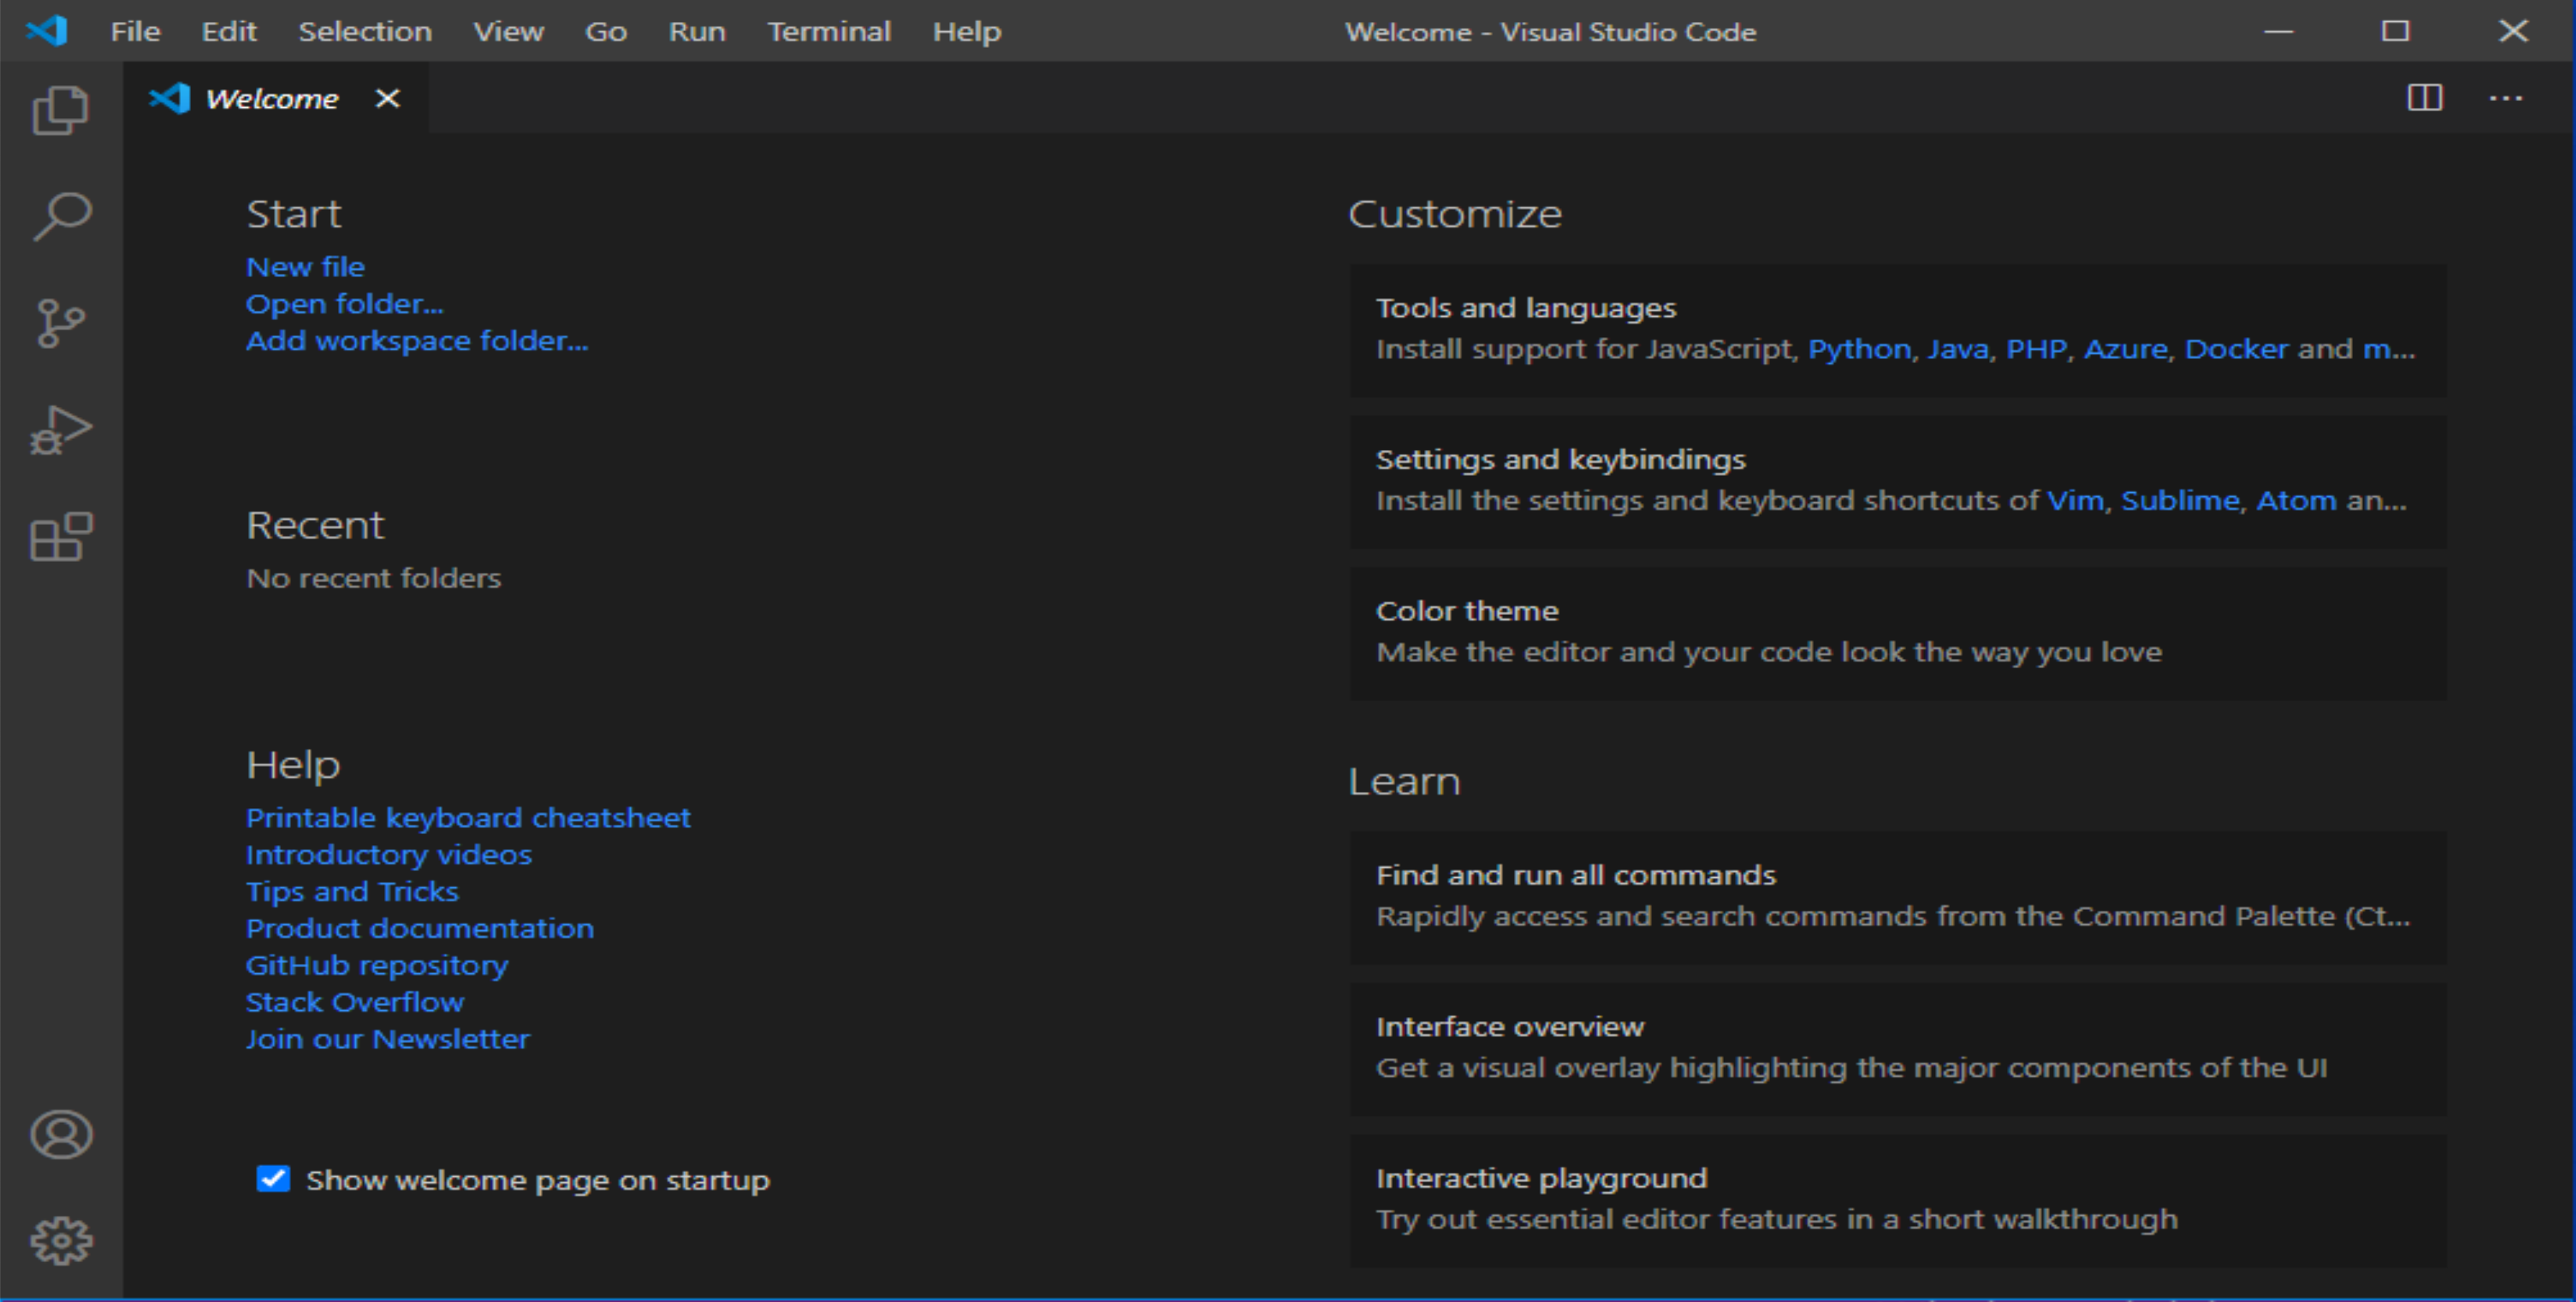
\includegraphics[keepaspectratio, width=0.9\linewidth]{chapters/08_ide/figures/vs_code_start.png}
            \caption{VS Code nach dem 1. Start}
        \end{figure}
    \end{frame}
    
    \begin{frame}{Visual Studio Code - Einrichtung (II)}
        Die Bearbeitung von Projekten/Dateien erfolgt in VS Code Workspacebasiert, d.h. es wird ein bestimmter Ordner als Workspace bestimmt, innerhalb dessen die Dateien verwaltet werden.\\~\
        
        Ein Workspace kann angelegt werden, indem direkt auf der Startseite \code{Add workspace folder...} oder unter \code{File} der Menüpunkt \code{Open Workspace...} ausgewählt wird.\\~\
        
        Hier bietet es sich an, einen Ordner zu erstellen, in dem alle Übungen und Codebeispiele gespeichert werden. Dieser Ordner dient dann als Workspace.
    \end{frame}
    
    \begin{frame}{Visual Studio Code - Einrichtung (III)}
        Nachdem der Workspace angelegt wurde, steht dieser zur Arbeit bereit. In der linken Leiste von VS Code gibt es verschiedene Reiter, der erste Reiter zeigt die Datei-/Ordnerstruktur des aktuellen Workspaces an. \\~\
        
        Durch einen Rechtsklick können so neue Ordner und Dateien angelegt werden
        
        \begin{figure}
            \centering
            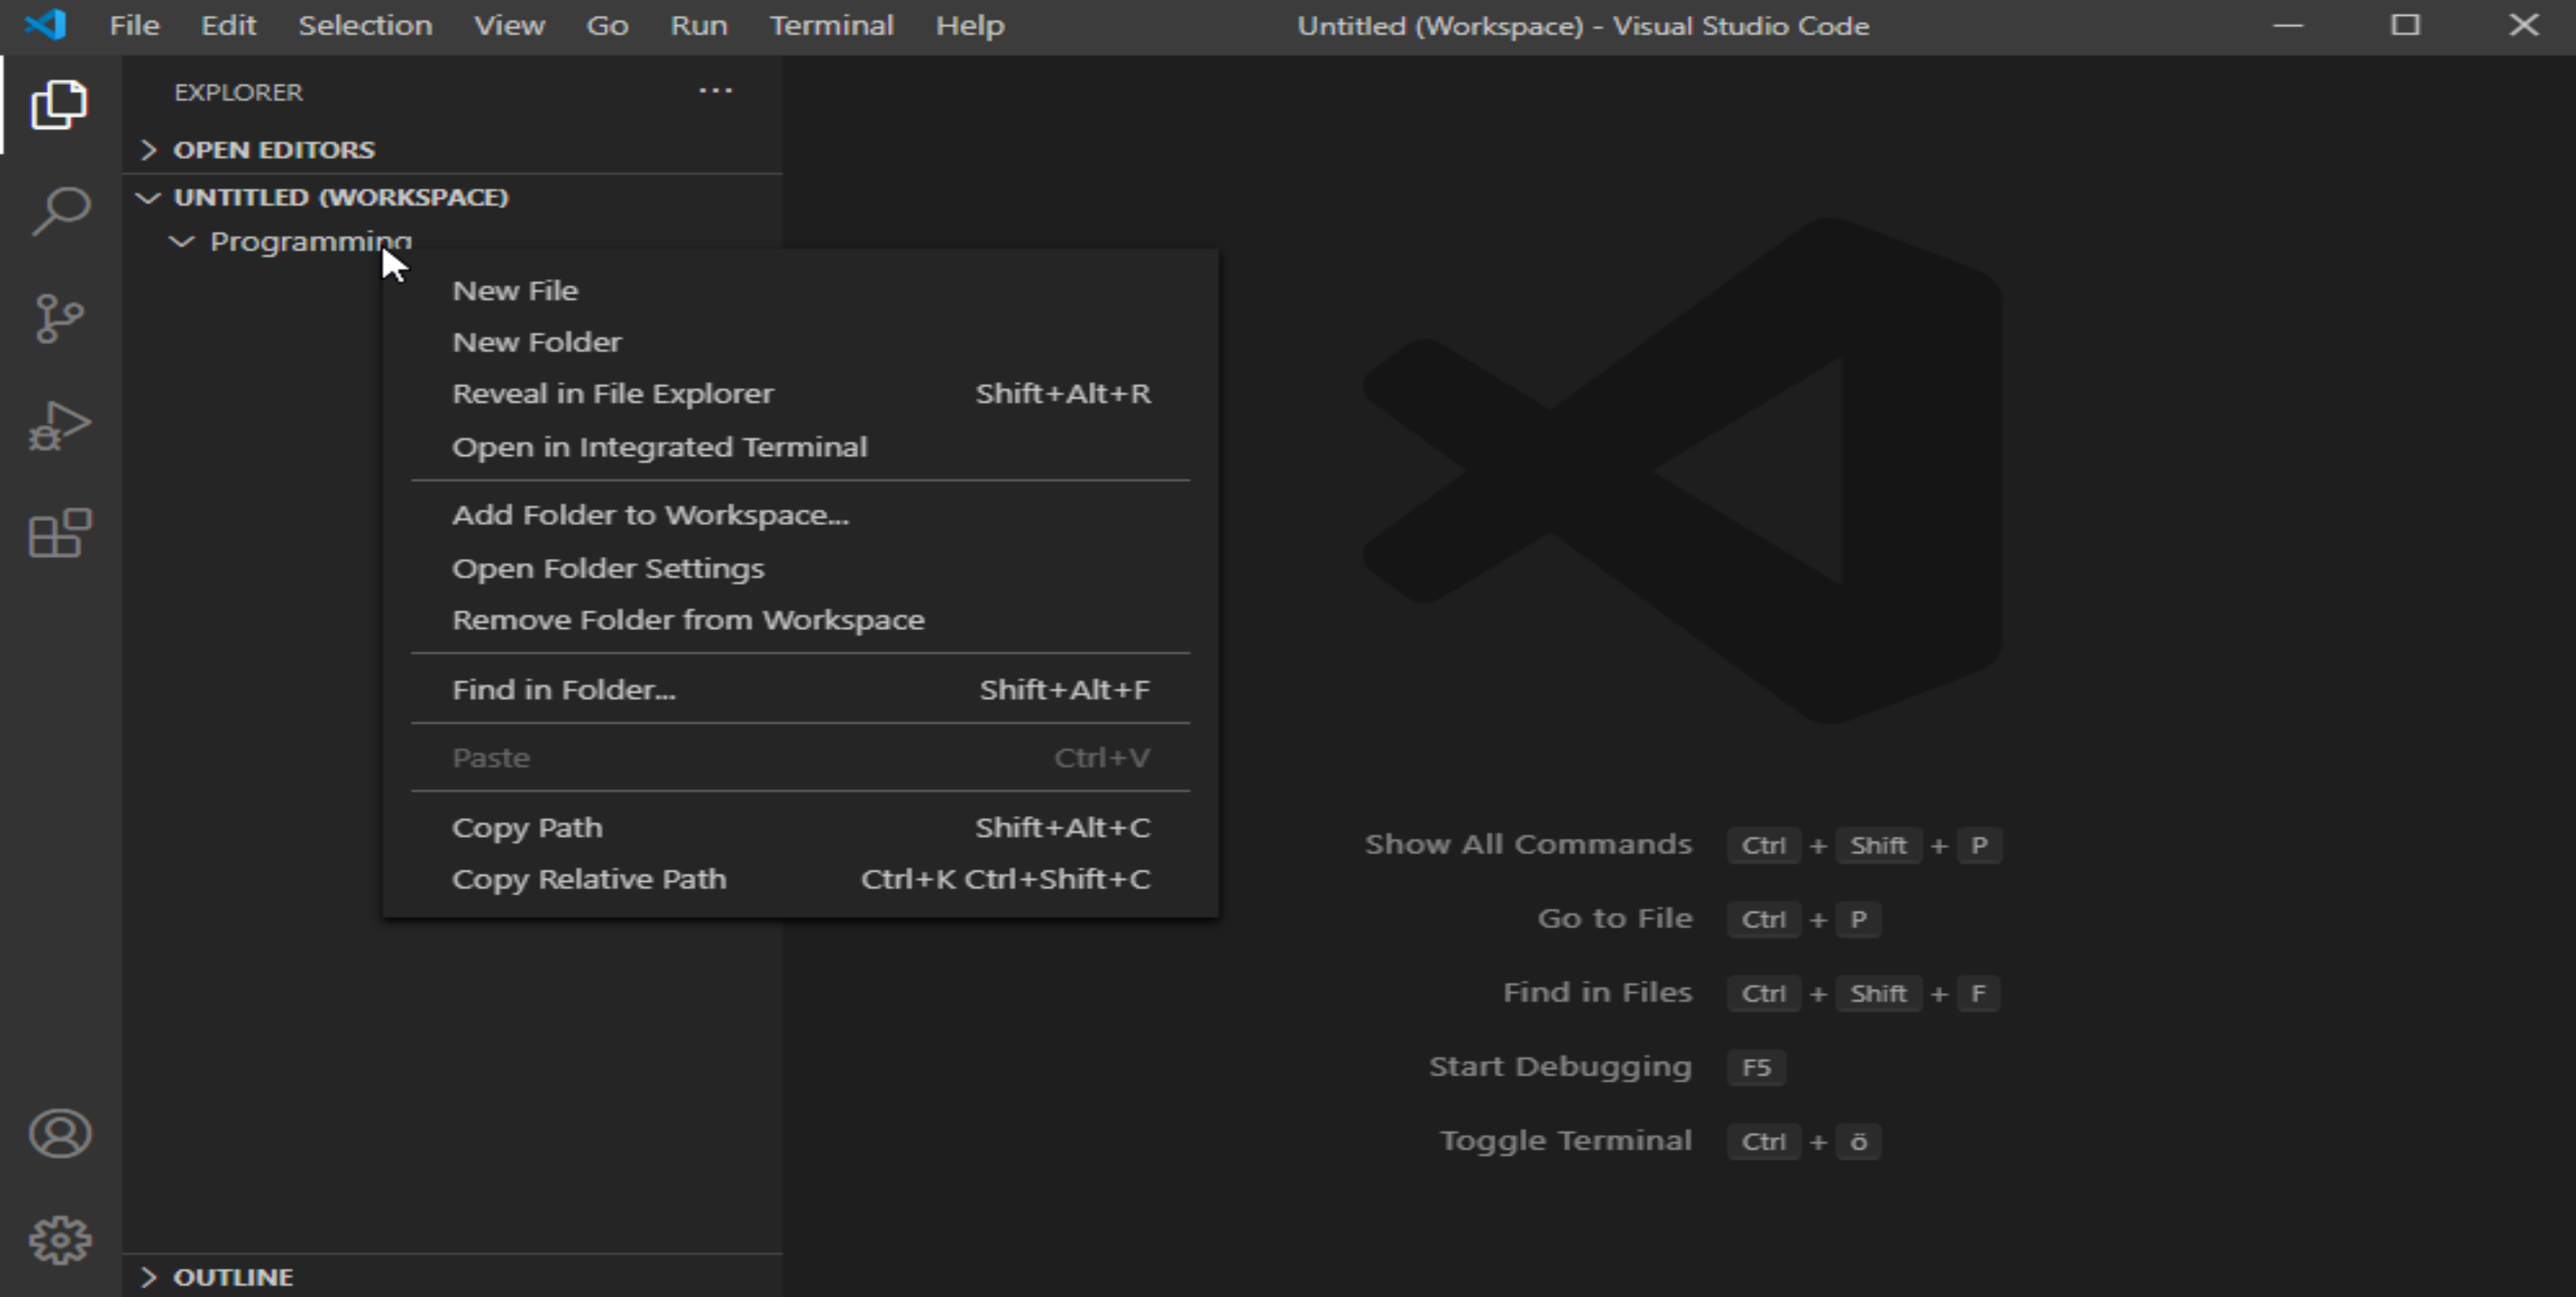
\includegraphics[keepaspectratio, width=0.9\linewidth]{chapters/08_ide/figures/vs_code_create_file.png}
            \caption{Anlegen einer neuen Datei oder Verzeichnisses}
        \end{figure}
    \end{frame}
    
     \begin{frame}{Visual Studio Code - Einrichtung (IV)}
        Wird eine neue \code{.py}-Datei angelegt, erkennt VS Code, dass es sich dabei um eine Python-Datei handelt und schlägt automatisch die Python-Erweiterung vor. Es wird empfohlen, diese zu installieren, um Python-spezifische Features zu aktivieren.
        
        \begin{figure}
            \centering
            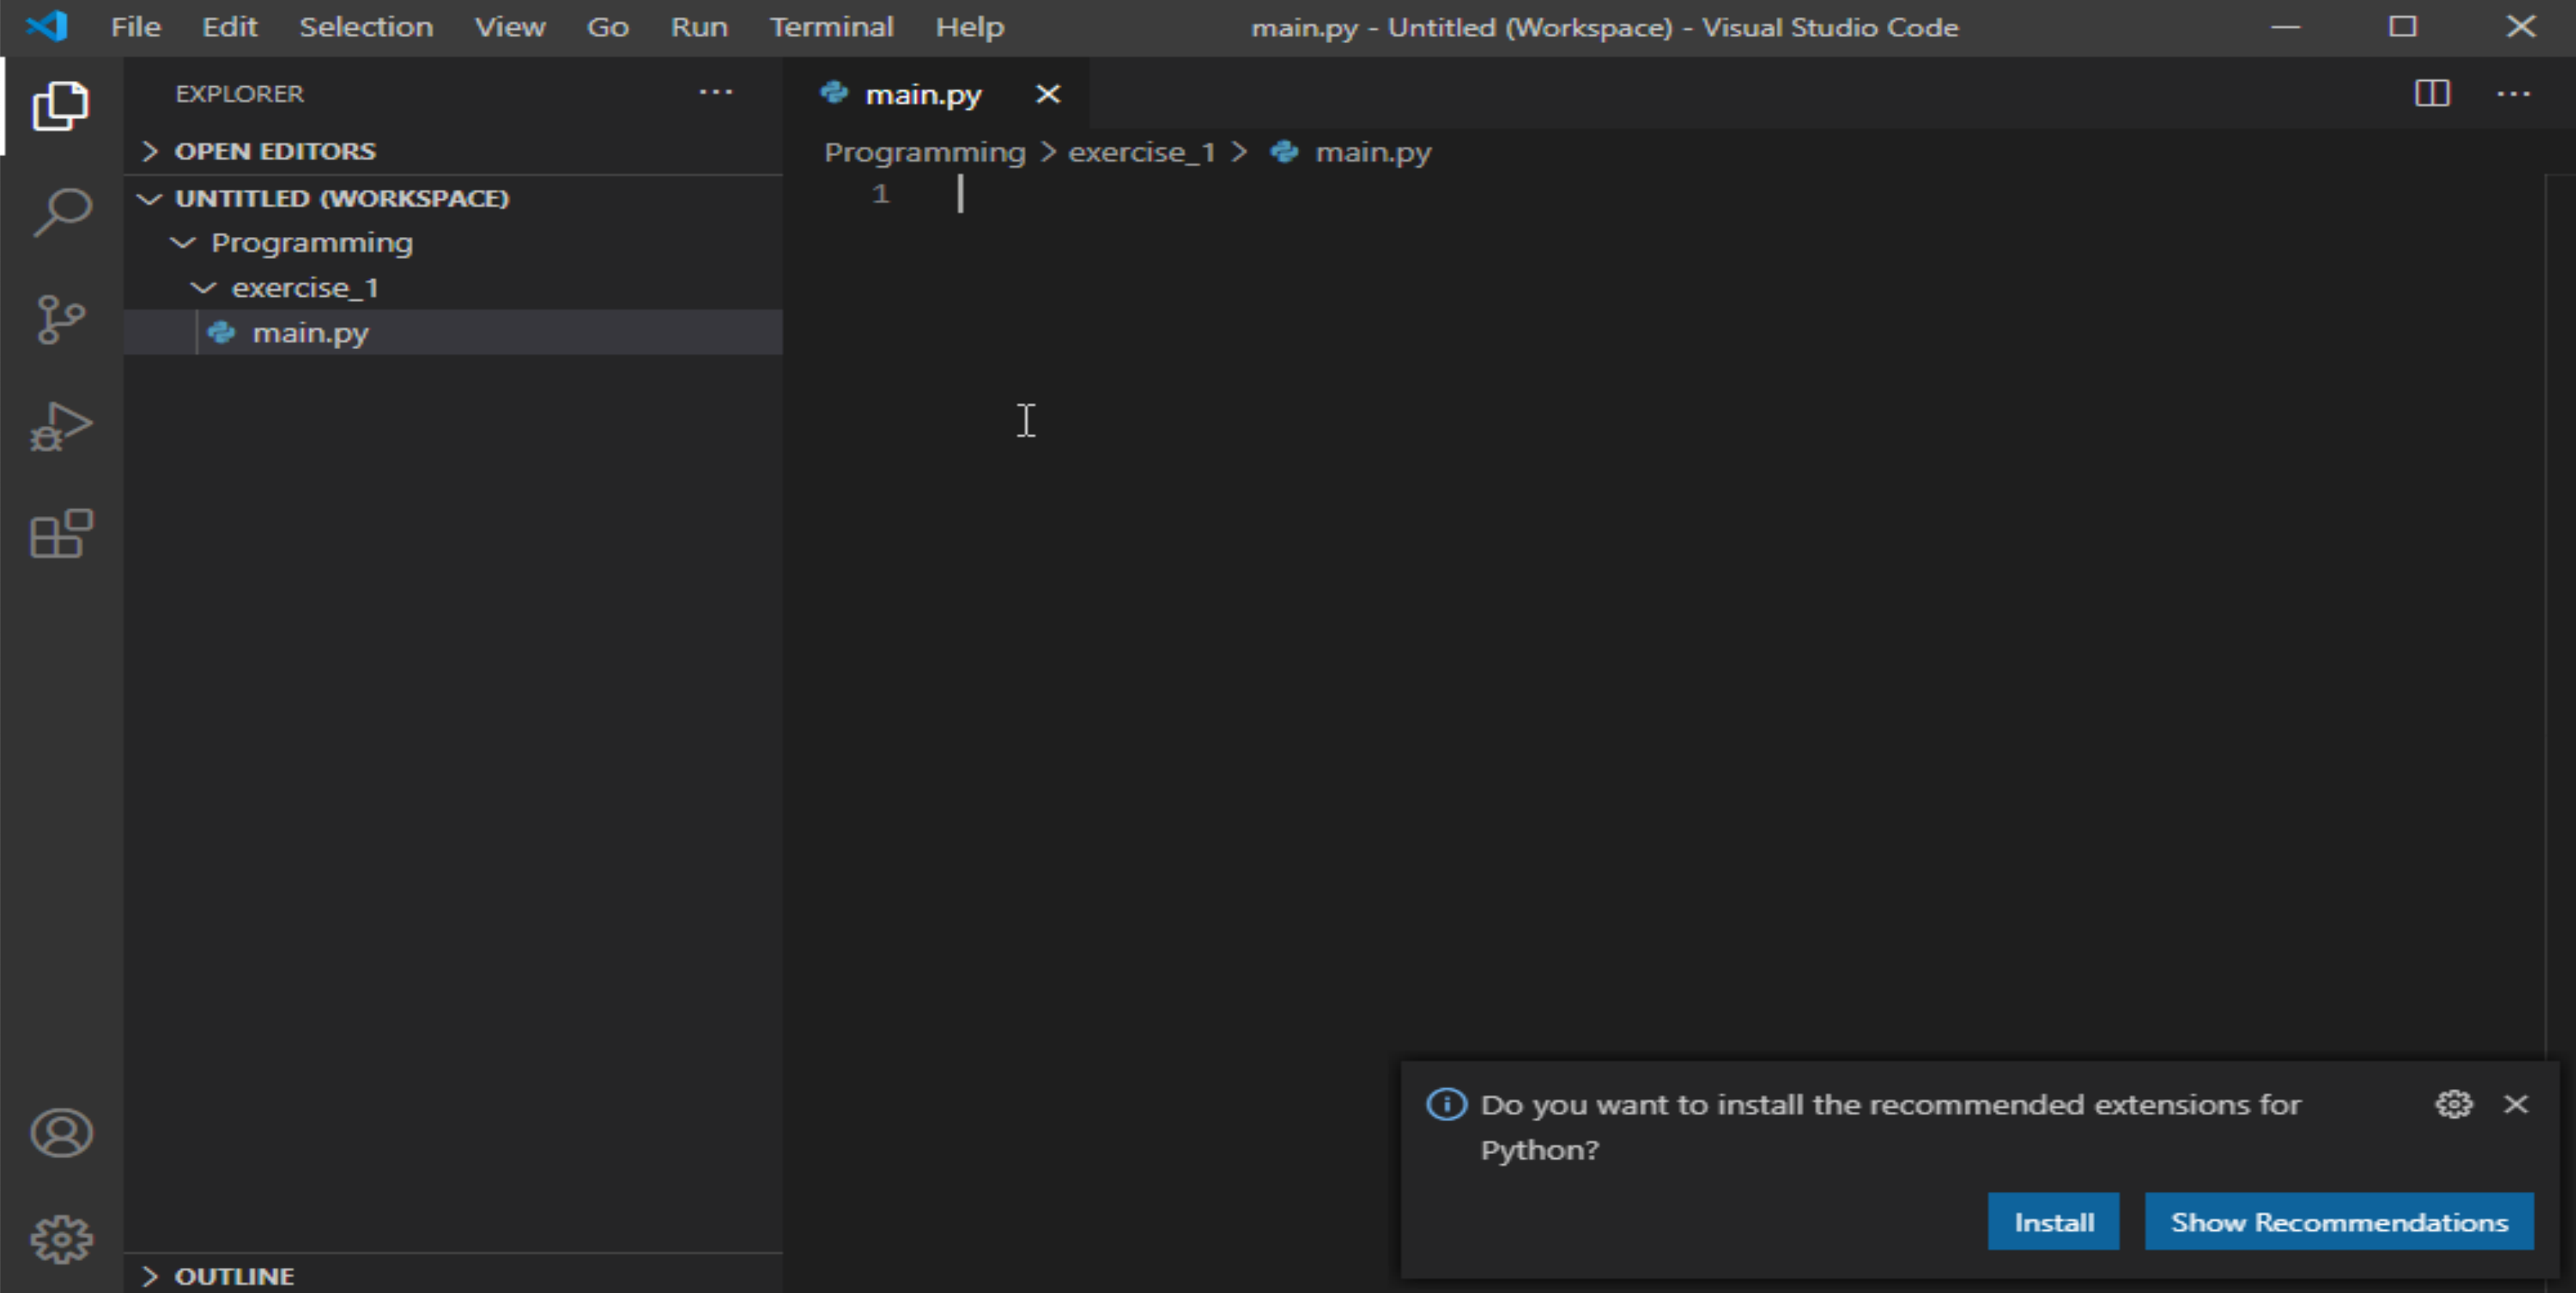
\includegraphics[keepaspectratio, width=0.9\linewidth]{chapters/08_ide/figures/vs_code_python.png}
            \caption{Vorschlag zur Installation der Python-Erweiterung}
        \end{figure}
        
    \end{frame}
    
    \begin{frame}{Visual Studio Code - Einrichtung (V)}
        Sobald die Python-Erweiterung installiert ist, wird automatisch ein installierter Python-Interpreter gesucht und links unten in der unteren Programmleiste angezeigt. Stellen Sie sicher, dass hier der korrekte Interpreter ausgewählt ist
        
        \begin{figure}
            \centering
            \includegraphics[keepaspectratio, width=0.9\linewidth]{chapters/08_ide/figures/vs_code_python_interpreter.png}
            \caption{Anzeige des aktuell verwendeten Python Interpreters}
        \end{figure}
        
    \end{frame}
    
        \begin{frame}{Visual Studio Code - Einrichtung (VI)}
        Wird nun eine Python Datei geöffnet, so kann diese direkt aus dem Editor heraus ausgeführt werden, indem das grüne Dreieck im oberen rechten Bereich gedrückt wird. Hierdurch wird die Konsole im unteren Bereich geöffnet, in der die Ausgabe erfolgt.
        
        \begin{figure}
            \centering
            \includegraphics[keepaspectratio, width=0.9\linewidth]{chapters/08_ide/figures/vs_code_python_run.png}
            \caption{Ausführen der Python Datei}
        \end{figure}
        
    \end{frame}
    
    \begin{frame}{Visual Studio Code - Einrichtung (VII)}
        Achtung: Wird hinter dem Dateinamen ein weißer Punkt angezeigt, bedeutet das, dass die Änderungen in der Datei noch nicht gespeichert wurden.
        
        \begin{figure}
            \centering
            \includegraphics[keepaspectratio, width=0.9\linewidth]{chapters/08_ide/figures/vs_code_not_saved.png}
            \caption{Ungespeicherte Änderungen in der Datei main.py}
        \end{figure}
        
    \end{frame}
\newcommand{\decktitle}{Python III - Kontrollstrukturen}

%%%%%%%%%%%%%%%%%%%%%%%%%%%%%%%%%%%%%%%%%%%%%%%%%
%
% DOCUMENT
%
%%%%%%%%%%%%%%%%%%%%%%%%%%%%%%%%%%%%%%%%%%%%%%%%%

\begin{frame}
    \subtitle{\decktitle}
    \titlepage
\end{frame}


\begin{frame}
    \frametitle{\textbf{Outline:}}
    \tableofcontents
\end{frame}

		
\section{Built-in Funktionen}
    \label{sec:builtin-func}

    \begin{frame}{Built-in Funktionen}
    
        Primär besteht die Aufgabe eines Entwicklers darin, sich konkrete oder abstrakte Lösungen zu einem bestehenden Problem zu überlegen und diese mithilfe eines Algorithmus in einer Programmiersprache umzusetzen. Häufig sind das Problem sowie die Lösung dabei so problemspezifisch, dass die Funktionalität hierfür in der gewünschten Form noch nicht existiert und deswegen vom Programmierer von Grund auf entwickelt werden muss. \\~\
        
        In der Regel sind Programme/Algorithmen aber so aufgebaut, dass komplexe Funktionalitäten aus der Komposition (Zusammensetzung) vieler einfacher Funktionen bestehen. Diese "einfachen" Funktionen sind so elementar und abstrakt, dass sie unabhängig vom konkreten Problem universell genutzt werden können. Daher ist es nicht sinnvoll, dass diese Elementarfunktionen, die sehr häufig benötigt werden, von jedem Entwickler von neuem geschrieben werden. Vielmehr enthalten die meisten Programmiersprachen bereits eine Menge verschiedener Grundfunktionen, die bereits fest in der Sprache integriert sind und daher ohne weitere Umstände von jedem Entwickler genutzt werden können. \\~\
        
        Diese Funktionen, die bereits mit der Installation des Python-Interpreters mitgeliefert werden, werden \textbf{Built-in Funktionen} genannt. 
        
    \end{frame}
    
    \begin{frame}{Built-in Funktionen}
        Python bietet eine große Zahl von Built-in Funktionen, die dem Entwickler zur Verfügung stehen, was eine schnelle und einfache Entwicklung ermöglicht. \\~\
        
        Die wichtigsten und hilfreichsten Built-in Funktionen werden im Folgenden vorgestellt. Einige dieser Built-in Funktionen sind bereits aus vorherigen Themengebieten bekannt. \\~\
        
        Eine komplette Übersicht aller eingebauten Funktionen findet sich in der offiziellen Dokumentation: \href{https://docs.python.org/3/library/functions.html}{https://docs.python.org/3/library/functions.html}
    \end{frame}    
    
    \begin{frame}[fragile]{Konvertierungsfunktionen und Konstruktoren}
        Funktionen, um Datentypenkonvertierungen (Casting) durchzuführen:
        
        \begin{itemize}
            \item \textbf{Numerische Typkonvertierungen:} \code{int(x)}, \code{float(x)}, \code{complex(x)}, \code{bool(x)}, \code{bin(x)}, ...
            
            \item \textbf{String Typkonvertierungen:} \code{str(x)}, \code{unicode(x)}, ...
            
            \item \textbf{Sequence Konstruktoren und Typkonvertierungen:} \code{list(x)}, \code{tuple(x)}, \code{range(x)}, ...
            
            \item \textbf{Map Konstruktoren und Typkonvertierungen:} \code{dict(x)}
            
            \item \textbf{Set Konstruktoren und Typkonvertierungen:} \code{set(x)}, \code{frozenset}
        \end{itemize}
    \end{frame}
    
    \begin{frame}[fragile]{Sequence Funktionen}
        Funktionen, die auf Sequence (und teilweise andere) Objekte angewendet werden können. \textbf{Das übergebene Sequence-Objekt \code{x} bleibt dabei jeweils unverändert}.
        
        \begin{itemize}
            \item \code{len(x)}: Anzahl der Elemente in der Sequence \code{x}
            
            \item \code{reversed(x)}: Erzeugt eine neue Sequence mit den gleichen Elementen in \code{x}, jedoch in umgekehrter Reihenfolge
            
            \item \code{sorted(x)}: Erzeugt eine neue Sequence mit den gleichen Elementen in \code{x}, jedoch in sortierter Reihenfolge (alphanumerische Sortierung)
            
            \item \code{sum(x)}: Erzeugt ein neues Skalar mit der Summe aller Elemente innerhalb der Sequence. Nur anwendbar auf numerische Sequence-Elemente.
            
            \item \code{zip(x)}: Erzeugt eine Sequence (zip-Objekt) von Tuples, in der jedes Tuple an Stelle $i$ das jeweils $i$-te Element der übergebenen Sequences enthält
            
\begin{pyconcode}
>>> result = zip([1,2,3], ['Alice', 'Bob', 'Carol'])
>>> print(list(result))
[(1, 'Alice'), (2, 'Bob'), (3, 'Carol')]
\end{pyconcode}            
        \end{itemize}
    \end{frame}
    
    \begin{frame}[fragile]{Input \& Output (I)}
        Elementare Funktionen zur Interaktion zwischen Mensch und System bzw. zur Eingabe und Ausgabe von Daten:
        
        \begin{itemize}
            \item \textbf{Ausgabe:} Um Werte (Numerische Werte, Strings, ...) auf der Standardausgabe auszugeben, wird \code{print()} verwendet.
            
            \item \textbf{Eingabe:} Analog existiert eine Funktion zur Eingabe von Werten: \code{input()}. Mithilfe dieser Funktionen können Werte von der Standardeingabe eingelesen werden, um beispielsweise Nutzereingaben abzufragen. Der \code{input()}-Funktion kann auch ein Parameter übergeben werden. Dabei handelt es sich um einen String, der dem Nutzer vor der Eingabe angezeigt wird ("Prompt"). Die Eingabe kann anschließend in einer Variable gespeichert werden.
            
\begin{pyconcode}
>>> x = input()
<<< Hello world
>>> print(x)
Hello world

>>> x = input("Please enter text: ")
<<< Bitte Text eingeben: Hello world
>>> print(x)
Hello world
\end{pyconcode}            
        \end{itemize}
    \end{frame}
    
    \begin{frame}[fragile]{Input \& Output (II)}
        \begin{alertblock}{Achtung}
            Da der Python-Interpreter nicht weiß, welchen Datentyp die Eingabe besitzen soll, wird die Eingabe standardmäßig als Strings eingelesen und gespeichert. 
            
            Soll jedoch ein anderer Datentyp eingelesen werden, z.B. eine Ganzzahl, muss der Wert nach der Eingabe mit der entsprechenden Funktion konvertiert werden
            
\begin{pyconcode}
>>> age = input("Please enter your age: ")
<<< Please enter your age: 20
>>> type(age)
<class 'str'>
>>> age = int(age)
>>> type(age)
<class 'int'>
\end{pyconcode}
        \end{alertblock}
    \end{frame}
    
    \begin{frame}[fragile]{Input \& Output (III)}
        \begin{itemize}
            \item \textbf{Eingabe:} Neben der Eingabe von Text können auch Dateien eingelesen werden. Hierzu steht die \code{open()}-Funktion zur Verfügung. Diese Funktion erwartet den Dateinamen (ggfs. inkl. Dateipfad, falls sich die Datei nicht im aktuellen Verzeichnis befindet.). Außerdem muss ggfs. der Modus angegeben werden: \code{'r'}, falls die Datei nur zum Lesen (Read) geöffnet wird, \code{'w'} zum Schreiben (Write)
            
\begin{pyconcode}
>>> content = open("main.py", "r")
>>> type(content)
<class '_io.TextIOWrapper'>
>>> lines = content.readlines()
>>> type(lines)
<class 'list'>
>>> print(lines)
['print("Hello world")\n']
\end{pyconcode}
        \end{itemize}
    \end{frame}
    
    \begin{subsection}{Aufgaben}
            \begin{frame}[fragile, allowframebreaks]{Aufgaben}
                \begin{enumerate}
                    \item Wozu gibt es die Built-in Funktionen?
                    \item Was ist nötig, um die Built-in Funktionen zu nutzen?
                    \item Es existieren zwei Tuples, die jeweils unterschiedliche Namen enthalten. Wie können daraus ganz einfach jeweils Paare von zwei Namen erzeugt werden?
                    \item Wo erscheint die Ausgabe von \code{print()}?
                    \item Was muss bei der \code{input()}-Funktion beachtet werden? Worin liegt der Unterschied zur \code{open()}-Funktion?
                    
                    \item Wie können mithilfe der \code{open()}-Funktion Dateiinhalte gelesen werden, die sich außerhalb des aktuellen Verzeichnisses befinden?
                    
                    \begin{block}{Hinweis}
                        Hinweis: Weitere Übungsaufgaben zum Themenblock 'Built-in Funktionen' finden sie im entsprechenden Übungsblatt.
                    \end{block}
                    
                    
                    
                \end{enumerate}
            \end{frame}
        \end{subsection}
    
\section{Steueranweisungen}
    
    \begin{frame}{Steueranweisungen}
        Mit den bis hierhin gelernten Funktionalitäten ist es bereits möglich, grundlegende und erweiterte Abläufe in Python umzusetzen. Von den eingangs vorgestellten Grundeigenschaften einer Programmiersprache sind nun bereits folgende Charakteristiken bekannt: \\~\
        
        \begin{itemize}
            \item Ein- und Ausgabe (\code{print()} und \code{input()} bzw. \code{open()})
            \item Variablendeklaration
            \item Mathematische Grundoperationen
            \item Zeichenkettenverarbeitung
        \end{itemize}
        
        Als letzte noch fehlende Eigenschaft werden im folgenden die unterschiedlichen Steueranweisungen vorgestellt und erläutert.
    \end{frame}
    
    \begin{frame}{Steueranweisungen}
        Mithilfe von Steueranweisungen kann der Ablauf eines Programms gesteuert werden. Somit ist es nun möglich, dass der Code nicht nur ausschließlich "von oben nach unten" durchläuft, sondern unterschiedliche Wege nehmen kann, an eine andere Stelle springt und dort fortgesetzt wird oder aber bestimmte Anweisungen mehrmals ausgeführt werden. \\~\
        
        Dies ermöglicht eine effiziente Programmierung, mit der der statische Ablauf ohne spezifische Anpassungen in eine dynamische, flexiblere Arbeitsweise wechselt. \\~\
        
        Es gibt unterschiedliche Arten von Steueranweisungen, die unterschiedliche Zwecke erfüllen. Die wichtigsten Steueranweisungen werden im Folgenden erläutert. Diese sind in fast jeder modernen Programmiersprache vorhanden, jedoch gibt es teilweise mehr oder weniger starke Abweichungen in der Syntax.
    \end{frame}
    
    \begin{subsection}{Conditionals}
        
        \begin{frame}{Conditionals}
            Die einfachste Art einer Steueranweisung sind \textbf{Conditionals} bzw. \textbf{Bedingte Anweisungen} oder auch \textbf{Verzweigungen} genannt. \\~\
            
            Hiermit kann der Ablauf des Codes beeinflusst werden, indem anhand von klar definierten Bedingungen unterschiedliche Codeabschnitte ausgeführt werden können. \\~\
            
            Conditionals sind eng mit den booleschen Werten verknüpft, da die Bedingungen jeweils als Wahrheitswert ausgewertet werden und daher entweder \code{True} oder \code{False} ergeben. \\~\
            
            Bedingte Anweisungen sind insbesondere dann unabdingbar, wenn mit dynamischen Informationen, wie etwa Dateneinspeisungen von anderen System oder Nutzereingaben gearbeitet wird, da hier die exakten Daten zur Zeit der Programmierung noch nicht bekannt sind und daher der Programmablauf dynamisch angepasst werden muss.
            
        \end{frame}
        
        \begin{frame}{if (I)}
            Die Conditionals folgen immer einem "Wenn Dann"-Schema, d.h. \textbf{wenn} die Bedingung wahr ist, \textbf{dann} wird der entsprechende Codeabschnitt ausgeführt. Andernfalls wird der Codeabschnitt übersprungen. \\~\
            
            Dementsprechend existiert in Python das Schlüsselwort \code{if}, mit dem eine Bedingung eingeleitet und entsprechend ausgewertet wird.\\~\
            
            Der Programmablauf folgt dabei der exemplarischen Darstellung \ref{fig:if}, die auf der nächsten Seite abgebildet ist.
        \end{frame}
        
        \begin{frame}{if (II)}
            \begin{figure}
                \centering
                \includegraphics[width=0.7\linewidth, keepaspectratio]{chapters/09_python3_control_flow/figures/if.png}
                \caption{Der Programmablauf mit einer Verzweigung}
                \label{fig:if}
            \end{figure}
        \end{frame}
    
        \begin{frame}[fragile]{if (III)}
            Die Syntax sieht dabei folgendermaßen aus:
            
\begin{pythoncode}
if <Bedingung>:
    # Anweisungen, die ausgeführt werden, wenn Bedingung wahr ist

# Anweisungen, die immer ausgeführt werden
\end{pythoncode}

            Hierbei sind mehrere Dinge zu beachten:
            
            \begin{itemize}
                \item Die Bedingung muss immer entweder \code{True} oder \code{False} sein. Auch Verknüpfungen von logischen Aussagen mit z.B. \code{and} sind zulässig
                \item Nach der Bedingung folgt immer ein Doppelpunkt. Hiermit wird verdeutlicht, dass im Folgenden die Anweisungen stehen, die ausgeführt werden, falls die Bedingung wahr ist
                \item Diese Bedingungen \textbf{müssen um eine Ebene} eingerückt sein, um den Anfang und das Ende des Blocks zu kennzeichnen
                \item Anweisungen außerhalb der if-Clause werden wieder ausgerückt
            \end{itemize}
        
        \end{frame}
        
        \begin{frame}[fragile]{if (IV)}
            
            \begin{exampleblock}{Beispiel}
            
\begin{pythoncode}
age = int(input("Bitte Alter eingeben: "))
if age >= 18:
    print("Der Nutzer ist volljährig")

print("Der Nutzer ist " + str(age) + " Jahre alt")
\end{pythoncode}

            \end{exampleblock}
        \end{frame}
        
        \begin{frame}[fragile]{if (V)}
            
            \begin{alertblock}{Achtung}
            
                Der interaktive Interpreter wertet im Normalfall jede Eingabe des Nutzer direkt aus. Nachdem der Nutzer aber eine if-Clause eingegeben hat, kann diese der Interpreter noch nicht ausführen, da er noch die Anweisungen erwartet, die ausgeführt werden sollen, falls die Bedingung wahr ist. Aus diesem Grund zeigt der Interpreter nach Eingabe der if-Clause zunächst \code{...} an, wodurch der Nutzer nun seine Anweisungen eingeben kann. Soll die if-Clause abgeschlossen werden, muss der Nutzer dies erneut mit der Enter-Taste bestätigen.

            \end{alertblock}
        \end{frame}
        
        \begin{frame}[fragile]{if-else (I)}
            In vielen Fällen soll nicht nur überprüft werden, ob eine Bedingung wahr ist, sondern auch Anweisungen ausgeführt werden, wenn dies nicht der Fall ist. Eine Möglichkeit besteht darin, die verneinte Aussage erneut zu überprüfen:
            
\begin{pythoncode}
age = int(input("Bitte Alter eingeben: "))
if age >= 18:
    print("Der Nutzer ist volljährig")

if age < 18:
    print("Der Nutzer ist nicht volljährig")
\end{pythoncode}

            Da dieses Vorgehen jedoch redundant ist gibt es hierfür eine häufig verwendete Kurzform: Das \textbf{if-else} Konstrukt 
                
        \end{frame}
        
        \begin{frame}[fragile]{if-else (II)}
            Mithilfe von \textbf{if-else} kann zunächst überprüft werden, ob eine Aussage wahr ist und dementsprechend Anweisungen ausgeführt werden. Ist die Aussage jedoch nicht wahr, werden die Anweisungen ausgeführt, die in der \code{else}-Clause enthalten sind \\~\
            
            Der Programmablauf folgt dabei der exemplarischen Darstellung \ref{fig:if-else}, die auf der nächsten Seite abgebildet ist.
        
        \end{frame}
        
         \begin{frame}[fragile]{if-else (III)}
            \begin{figure}
                \centering
                \includegraphics[width=0.7\linewidth, keepaspectratio]{chapters/09_python3_control_flow/figures/if-else.png}
                \caption{Der Programmablauf mit einer if-else Verzweigung}
                \label{fig:if-else}
            \end{figure}
         \end{frame}
         
        \begin{frame}[fragile]{if-else (IV)}
            Die Syntax sieht dabei folgendermaßen aus:
            
\begin{pythoncode}
if <Bedingung>:
    # Anweisungen, die ausgeführt werden, wenn Bedingung wahr ist
else:
    # Anweisungen, die ausgeführt werden, wenn Bedingung falsch ist
    
# Anweisungen, die immer ausgeführt werden
\end{pythoncode}

            Hierbei sind mehrere Dinge zu beachten:
            
            \begin{itemize}
                \item Bei der else-Clause wird nie eine Bedingung überprüft, da diese automatisch ausgeführt wird, falls die Bedingung der if-Clause zu \code{False} auswertet.
                \item Es wird \textbf{entweder} die if-Clause oder \textbf{oder} die else-Clause ausgeführt. Es ist nicht möglich, dass keine der beiden oder  beide gleichzeitig ausgeführt werden.
                \item Nach den Anweisungen der if-Clause muss eine Ausrückung erfolgen, da hier ein neuer Block beginnt. Die Anweisungen der else-Clause werden dann wieder eingerückt.
                \item Eine else-Clause ist immer optional
            \end{itemize}
        
        \end{frame}
        
        \begin{frame}[fragile]{if-else (V)}
            
            \begin{exampleblock}{Beispiel}
            
\begin{pythoncode}
age = int(input("Bitte Alter eingeben: "))
if age >= 18:
    print("Der Nutzer ist volljährig")
else: 
    print("Der Nutzer ist nicht volljährig")

print("Der Nutzer ist " + str(age) + " Jahre alt")
\end{pythoncode}

            \end{exampleblock}
        \end{frame}
        
        
        \begin{frame}[fragile]{if-elif-else (I)}
            Um komplexere Abfragen noch einfacher umsetzen zu können, gibt es eine Erweiterung des \code{if} bzw. \code{if-else} Konstrukts:\\~\
            
            Mithilfe von else-if (Keyword: \code{elif}) können beliebig viele Aussagen auf ihren Wahrheitswert überprüft werden. Sobald eine dieser Aussagen wahr ist, werden die entsprechenden Anweisungen ausgeführt. Die nachfolgenden \code{elif}-Clauses werden dann nicht mehr überprüft, auch die \code{else}-Anweisungen werden dann nicht mehr ausgeführt. \\~\
            
            Der Programmablauf folgt dabei der exemplarischen Darstellung \ref{fig:elif}, die auf der nächsten Seite abgebildet ist.
        \end{frame}
        
        \begin{frame}[fragile]{if-elif-else (II)}
            \begin{figure}
                \centering
                \includegraphics[width=0.7\linewidth,height=0.7\textheight,keepaspectratio]{chapters/09_python3_control_flow/figures/elif.png}
                \caption{Der Programmablauf mit einer if-elif-else Verzweigung}
                \label{fig:elif}
            \end{figure}
         \end{frame}
         
         \begin{frame}[fragile]{if-elif-else (III)}
            Die Syntax sieht dabei folgendermaßen aus:
            
\begin{pythoncode}
if <Bedingung 1>:
    # Anweisungen, die ausgeführt werden, wenn Bedingung 1 wahr ist
elif <Bedingung 2>:
    # Anweisungen, die ausgeführt werden, wenn Bedingung 2 wahr und Bedingung 1 falsch ist
elif <Bedingung 3>:
    # Anweisungen, die ausgeführt werden, wenn Bedingung 3 wahr und Bedingung 1 und Bedingung 2 falsch sind
else:
    # Anweisungen, die ausgeführt werden, wenn alle Bedingungen falsch sind
    
# Anweisungen, die immer ausgeführt werden
\end{pythoncode}

            Hierbei sind mehrere Dinge zu beachten:
            
            \begin{itemize}
                \item Es werden die Bedingungen der Reihe nach geprüft. Die Anweisungen der ersten Bedingung, die \code{True} ergibt, werden ausgeführt, die restlichen \code{elif} bzw. \code{else}-Statements ignoriert.
                \item Wertet keine der \code{if} oder \code{elif}-Clauses zu \code{True} aus, wird die \code{else}-Clause ausgeführt (falls vorhanden)
                \item Auch hier ist die \code{else}-Clause optional
            \end{itemize}
        
        \end{frame}
        
        \begin{frame}[fragile]{if-elif-else (IV)}
            
            \begin{exampleblock}{Beispiel}
            
\begin{pythoncode}
age = int(input("Bitte Alter eingeben: "))
if age > 18:
    print("Der Nutzer ist volljährig")
elif age == 18:
    print("Der Nutzer ist dieses Jahr volljährig geworden.")
else: 
    print("Der Nutzer ist nicht volljährig")

print("Der Nutzer ist " + str(age) + " Jahre alt")
\end{pythoncode}

            \end{exampleblock}
        \end{frame}
        
        \begin{frame}{Verschachtelte Conditionals (I)}
            Bedingte Anweisungsblöcke können auch verschachtelt werden, d.h. in einer \code{if}, \code{elif} oder \code{else}-Clause können wiederum weitere bedingte Anweisungen enthalten sein.  \\~\
            
            Eine (praktische) Maximalzahl an erlaubten Verschachtelungen gibt es nicht.
            
        \end{frame}
        
        \begin{frame}{Verschachtelte Conditionals (II)}
            \begin{alertblock}{Achtung}
                Für jeden Anweisungsblock muss der Code um eine Ebene eingerückt werden. Enthält also beispielsweise eine \code{if}-Clause eine weitere \code{if}-Clause, muss der Code um 2 Ebenen eingerückt werden.
            \end{alertblock}
        \end{frame}
        
          \begin{frame}[fragile]{Verschachtelte Conditionals (III)}
            \begin{exampleblock}{Beispiel}
\begin{pythoncode}
username = int(input("Bitte Benutzername eingeben: "))
password = input("Bitte Passwort eingeben: ")

if username in  ["Alice", "Bob", "Carol"]:
    if len(password) < 6:
        print("Das Passwort ist unsicher")
    else:
        print("Der Nutzer " + username + " existiert und das Passwort ist sicher")
else:
    print("Der Nutzername ist nicht bekannt")
\end{pythoncode}
            \end{exampleblock}
        \end{frame}
        
    
    \begin{subsubsection}{Aufgaben}
        \begin{frame}[fragile, allowframebreaks]{Aufgaben}
            \begin{enumerate}
                \item Wofür werden Conditionals benötigt?
                \item Kann jede Funktionalität der Conditionals auch ohne Conditionals genutzt werden?
                \item Warum gibt es Einrückungen?
                \item Können bei Conditionals auch andere Datenwerte als boolesche Werte auf Wahrheit getestet werden?
                \item Warum werden bei else-Clauses keine Bedingungen abgefragt?
                \item Wie viele Anweisungen darf eine if-Clause besitzen?
                \item Kann eine \code{elif}-Clause auch anders ausgedrückt werden?
                \item Werden stets alle Bedingungen eines if-elif-else-Konstrukts überprüft?
                \item Was muss bei der Verschachtelung von Conditionals beachtet werden?
                
               \begin{block}{Hinweis}
                Hinweis: Weitere Übungsaufgaben zum Themenblock 'Conditionals' finden sie im entsprechenden Übungsblatt.
            \end{block}
            
            \end{enumerate}
        \end{frame}
    \end{subsubsection}
% Kurzschreibweise
    \end{subsection}
    
    \begin{subsection}{Schleifen}
        
        \begin{frame}{Schleifen (I)}
            Schleifen stellen in der Programmierung ein wichtiges Werkzeug dar, das zu einer effizienten, schnellen und einfachen Entwicklung beiträgt. \\~\
            
            Der Sinn einer Schleife besteht darin, eine Anweisung mehrmals auszuführen, ohne jede einzelne dieser Anweisungen "hartgecoded" (also explizit aufgeführt) in den Programmcode zu schreiben. \\~\
            
            Schleifen werden häufig auch \textit{Loops} genannt.
        \end{frame}
        
        \begin{frame}[fragile]{Schleifen (II)}
        
            Im Folgenden ist ein Beispiel dargestellt, wie alle Elemente einer Liste (ohne Schleife) der Reihe nach ausgegeben werden: 
            
            \begin{exampleblock}{Beispiel}
\begin{pythoncode}
names = ['Alice', 'Bob', 'Carol', 'Dave']
index = 0

print(names[index])
index = index+1
print(names[index])
index = index+1
print(names[index])
index = index+1
print(names[index])
\end{pythoncode}            
            \end{exampleblock}
            
            Hier ist deutlich zu erkennen, dass diese Art der Ausgabe aller Listenelemente sehr ineffizient ist. Insbesondere bei längeren Listen ist eine solche Vorgehensweise unpraktikabel.
        \end{frame}
        
        \begin{frame}[fragile]{Schleifen (III)}
            Abhilfe hierfür schaffen Schleifen, da mit diesen wiederkehrende Anweisungen nur einmal angegeben werden müssen und diese dann beliebig oft ausgeführt werden kann. \\~\
            
            Generell gibt es in Python zwei Arten von Schleifen: \code{while}-Schleifen und \code{for}-Schleifen. \\~\
            
            Die Funktionsweise der beiden Schleifentypen ist sehr ähnlich, mit beiden Arten können jeweils die gleichen Funktionalitäten umgesetzt werden. Jedoch gibt es feine Unterschiede, durch die sich \code{for} und \code{while}-Schleifen unterscheiden und sich je nach Anwendungsfall der eine oder der andere Typ eher anbietet.
        \end{frame}
        
        \begin{frame}[fragile]{Schleifen (IV)}
            Alle Schleifen folgen dem gleichen Ablauf:
                
                \begin{enumerate}
                    \item Prüfe, ob die Abbruchbedingung der Schleife erfüllt ist. Falls nicht, gehe zu Schritt 2
                    \item Führe die Anweisungen aus, die im Schleifenrumpf enthalten sind. Anschließend gehe zu Schritt 1.
                \end{enumerate}
        \end{frame}
        
        
        
        \begin{frame}[fragile]{while (I)}
            Mithilfe von \code{while}-Schleifen können Anweisungen solange ausgeführt werden, solange die Anweisung im Schleifenkopf wahr ist. \\~\
            
            Das bedeutet, dass der Entwickler sich zunächst überlegen muss, was das \textbf{Abbruchkriterium} ist.
            
            Die Syntax des \code{while}-Loops sieht folgendermaßen aus:
            
\begin{pythoncode}
while <Bedingung>:
    # Anweisungen, die ausgeführt werden, solange die Bedingung wahr ist

# Anweisungen, die ausgeführt werden, nachdem die Schleife beendet wurde / durchgelaufen ist
\end{pythoncode}
        \end{frame}
        
        \begin{frame}{while (II)}
            Die Bedingung, die im Schleifenkopf angegeben wird, muss stets ein boolescher Ausdruck sein, die entweder \code{True} oder \code{False} ergibt. Sobald die Anweisung zu \code{False} ausgewertet wird, ist die Schleife beendet und der Codeablauf wird fortgesetzt. \\~\
            
            \code{while}-Schleifen werden i.d.R. dann verwendet, wenn eine Anweisung bestimmt oft (x Mal) ausgeführt werden soll.
            
        \end{frame}
        
        \begin{frame}{while (III)}
            \begin{alertblock}{Achtung}
                \code{while}-Schleifen sind \textbf{kopfgesteuerte} Schleifen. Das bedeutet, dass die Abbruchbedingung \textbf{vor} jedem Schleifendurchgang überprüft wird. Wenn die Bedingung \code{False} ist, wird der nächste Schleifendurchgang nicht mehr ausgeführt.
                Es gibt auch \textbf{fußgesteuerte} Schleifen, bei denen \textbf{nach} jedem Durchgang die Bedingung geprüft wird und abhängig davon der nächste Schleifendurchgang gestartet wird. \\~\
                
                Das hat zur Folge, dass fußgesteuerte Schleifen mindestens einmal durchlaufen werden, bei kopfgesteuerten Schleifen ist es auch möglich, dass kein Schleifendurchlauf stattfindet.
            \end{alertblock}
        \end{frame}
        
        \begin{frame}[fragile]{while (IV)}
                \begin{exampleblock}{Beispiel}
                
                Im folgenden Codeausschnitt sollen die Zahlen von 0 bis 5 in absteigender Reihenfolge ausgegeben werden, ohne die expliziten Werte anzugeben:
\begin{pyconcode}
>>> i = 5
>>> while i >= 0:
>>>     print(i)
>>>     i = i-1

5
4
3
2
1
0
\end{pyconcode}                
                \end{exampleblock}
        \end{frame}
        
        \begin{frame}[fragile]{while (V)}
            \begin{alertblock}{Achtung}
                Die Anweisung \code{i = i-1} im vorherigen Beispiel ist sehr wichtig, da hierdurch die Variable \code{i} um den Wert 1 verringert wird. Wird diese Anweisung vergessen, wird bei jedem Schleifendurchgang überprüft, ob \code{i>0} wahr ist. Da sich \code{i} nicht ändert, wird stets überprüft ob \code{5 > 0} wahr ist, was immer der Fall ist. Dies hat eine \textbf{Endlosschleife} zur Folge, da die Abbruchbedingung nie erreicht wird.
            \end{alertblock}
        \end{frame}
        
        \begin{frame}{for (I)}
        
            Neben den \code{while} Schleifen gibt es noch eine weitere Schleifenart: Die \code{for} Schleife. \\~\
            
            Anders als \code{while} Schleifen sind \code{for} Schleifen nicht zähler- sondern elementbasiert. Der Vorteil liegt darin, dass so ein Durchlaufen (Iterieren) aller Elemente einer Liste oder listenähnlichen Struktur sehr einfach ist. \\~\
            
            Die Gefahr, dass der Entwickler vergisst, eine Zählvariable zu in-/dekrementieren und so eine Endlosschleife zu erzeugen, sinkt.
            
        \end{frame}
        
        
        \begin{frame}[fragile]{for (II)}
            Die Syntax einer \code{for}-Schleife ist folgendermaßen:
            
\begin{pythoncode}
for <Elementvariable> in <Sequence>:
    # Anweisungen, die für jedes Element der Sequence ausgeführt werden

# Anweisungen, die nach Durchlaufen der Schleife ausgeführt werden
\end{pythoncode} \\~\

            Bei \code{for} Schleifen wird über jedes Element der Sequenz iteriert, welches automatisch einer Variablen (oben \code{<Elementvariable>}) zugewiesen wird.\\~\
            
            Im Gegensatz zur \code{while} Schleife muss der Entwickler hier also keine explizite Abbruchbedingung angeben, sondern der Schleifendurchlauf endet, wenn alle Elemente der Sequenz ein Mal durchlaufen wurden.
        \end{frame}
        
        \begin{frame}[fragile]{for (III)}
            \begin{exampleblock}{Beispiel}
            
            Im folgenden Codeausschnitt sollen die Namen, die in der Liste enthalten sind, ausgegeben werden:
            
\begin{pythoncode}
names = ['Alice', 'Bob', 'Carol', 'Eve', 'Dave']

for name in names:
    print(name)

Alice
Bob
Carol
Eve
Dave
\end{pythoncode}

            Der Name der Variablen \code{name} als Variable für das jeweilige Listenelement kann frei gewählt werden \footnote{solange er den Regeln der Variablenbenennung entspricht}
            
            \end{exampleblock}
        \end{frame}
        
        \begin{frame}[fragile]{range (I)}
            Eine der am häufigsten im Zusammenhang mit der \code{for} Schleife genutzten Built-In Funktionen ist \code{range()}. \\~\
            
            Mithilfe von \code{range()} können einfach Sequenzen von Zahlen erzeugt werden. \\~\
            
            Wird der \code{range()}-Funktion nur ein Parameter übergeben, wird eine Sequenz von Zahlen von 0 bis zur entsprechenden Zahl erzeugt:
            
\begin{pyconcode}
>>> intervall = range(5)
>>> type(intervall)
<class 'range'>

>>> intervall_list = list(intervall)
>>> type(intervall_list)
<class 'list'>
>>> print(intervall_list)
[0, 1, 2, 3, 4]
\end{pyconcode}

        \end{frame}
        
        \begin{frame}[fragile]{range (II)}
             Werden der \code{range()}-Funktion 2 Parameter übergeben, wird eine Sequenz von Zahlen vom Anfangswert (Parameter 1) bis zum Endwert (Parameter 2) erzeugt:

\begin{pythoncode}
intervall = range(5,12)
for number in intervall:
    print(number)

5
6
7
8
9
10
11
\end{pythoncode}             
        \end{frame}
        
        \begin{frame}[fragile]{range (III)}
             Werden der \code{range()}-Funktion 3 Parameter übergeben, wird eine Sequenz von Zahlen vom Anfangswert (Parameter 1) bis zum Endwert (Parameter 2) mit einer Schrittweite (Parameter 3) erzeugt:

\begin{pythoncode}
intervall = range(5,12,2)
for number in intervall:
    print(number)

5
7
9
11
\end{pythoncode}        

            Wird keine Schrittweite angegeben, wird automatisch der Standartwert 1 verwendet.
             
        \end{frame}
        
        \begin{frame}{range (IV)}
        
           \begin{alertblock}{Achtung}
                Bei der \code{range()}-Funktion ist der Anfangswert stets inklusiv, der Endwert immer exklusiv. \code{range(2,7)} beinhaltet also alle Zahlen zwischen 2 und 6.
            \end{alertblock}  
        \end{frame}
        
        \begin{frame}[fragile]{range (V)}
        
            Die \code{range()}-Funktion wird häufig in Kombination mit der \code{for} Schleife genutzt, da so die Funktionalität einer zählerbasierten \code{while} Schleife nachgebildet werden kann, ohne sich um die Initialisierung und Inkrementierung des Zählers kümmern zu müssen.
            
            \begin{exampleblock}{Beispiel}
                Mit der folgenden \code{while} Schleife werden die Zahlen von 1 - 20 ausgegeben:
                
\begin{pythoncode}
i = 1
while i<=20:
    print(i)
    i = i+1
\end{pythoncode}
                Die selbe Funktionalität kann mit folgender \code{for} Schleife in Kombination einfacher und übersichtlicher umgesetzt werden:

\begin{pythoncode}
for i in range(1, 21):
    print(i)
\end{pythoncode}               
                
            \end{exampleblock}
        \end{frame}

            
        
        
        \begin{frame}{continue - Iterationsabbruch (I)}
            Es gibt zwei Hilfsanweisungen, die bei der Entwicklung von Schleifen hilfreich sein können. Hierzu gehört \code{continue}.\\~\
            
            Die \code{continue} Anweisung wird genutzt, falls der aktuelle Iterationsdurchgang abgebrochen werden und mit dem nächsten Iterationsdurchgang weitergemacht werden soll (solange die Abbruchbedingung nicht erfüllt ist). \\~\
            
            Oft wird die \code{continue}-Anweisung zu den schlechten Codepraktiken gezählt, da es deutlich schwieriger werden kann, als Mensch den Programmablauf nachzuvollziehen. Aus diesem Grund sollte auf \code{continue} verzichtet werden falls möglich
        \end{frame}
        
        \begin{frame}[fragile]{continue - Iterationsabbruch (II)}
            
            \begin{exampleblock}{Beispiel}
                Im folgenden Beispiel wird für die Zahlen von 2 - 10 überprüft, ob sie gerade oder ungerade sind:
                
\begin{pythoncode}
for num in range(2, 10):
    if num % 2 == 0:
        print("Gerade Zahl gefunden")
        continue
    print("Ungerade Zahl gefunden")
\end{pythoncode}
                
                \textbf{Dieser Codeausschnitt soll lediglich die Funktionsweise von \code{continue} verdeutlichen. Der abgebildete Code sollte so nicht verwendet werden, da er unnötig umständlich ist. Eine einfachere und bessere Variante stellt hier eine Implementierung mit if-else dar.}
            \end{exampleblock}
        \end{frame}
        
        \begin{frame}{break - Schleifenabbruch (I)}
            Neben \code{continue} gibt es noch eine weitere Hilfsanweisung:  \code{break}.\\~\
            
            Die \code{break} Anweisung wird genutzt, um das Durchlaufen der Schleife abzubrechen, auch wenn die Abbruchbedingung noch nicht erfüllt ist. Im Gegensatz zu \code{continue} wird also nicht nur die aktuelle Iteration, sondern die komplette Schleife abgebrochen.  \\~\
            
            Auch \code{break} sollte nur genutzt werden, wenn die Anweisung wirklich benötigt wird, andernfalls sollten eindeutigere Codeumsetzungen bevorzugt werden.
        \end{frame}
        
        \begin{frame}[fragile]{break - Schleifenabbruch (II)}
            
            \begin{exampleblock}{Beispiel}
                Im folgenden Beispiel wird für die Zahlen ab 100 überprüft, ob sie durch 7 teilbar sind. Falls das der Fall ist, wird die Schleife abgebrochen:
                
\begin{pythoncode}
index = 100
divider = 7
while True:
    if index % divider == 0:
        print(str(index) + " ist teilbar durch " + str(divider))
        break
    else:
        print(str(index) + " ist nicht teilbar durch " + str(divider))
        index = index +1
\end{pythoncode}
            
            \end{exampleblock}
        \end{frame}

        \begin{subsubsection}{Aufgaben}
            \begin{frame}[fragile, allowframebreaks]{Aufgaben}
                \begin{enumerate}
                    \item Wofür sind Schleifen hilfreich?
                    \item Welche Arten von Schleifen gibt es? Was sind die Unterschiede?
                    \item Welche kopfgesteuerten bzw. fußgesteuerten Schleifen gibt es in Python?
                    \item Wann werden primär \code{while} und wann \code{for} Schleifen genutzt?
                    \item Was muss bei \code{while} Schleifen unbedingt beachtet werden? Warum ist das bei \code{for} Schleifen nicht relevant?
                    
                    \item Welche Funktionalität bietet die \code{range()}-Funktion?
                    \item Warum wird beim Erzeugen einer Range eine Variable des Typs \code{range} und nicht \code{list} erzeugt?
                    \item Was muss beim Erzeugen einer \code{range} beim Start- und Endwert beachtet werden?
                    \item Was ist das Ergebnis der Anweisung \code{list(range(20,0,-2))}?
                    
                    \item Wozu wird \code{continue} genutzt und warum sollte es vermieden werden?
                
                    
                \end{enumerate}
            \end{frame}
        \end{subsubsection}
    \end{subsection}
    
    
\section{Funktionen}
    
    \begin{frame}{Funktionen}
        Funktionen gehören zu den Grundkonzepten einer Programmiersprache und sind in so gut wie allen Programmiersprachen vorhanden und verwendbar. \~\\
        
        Sie stellen ein wichtiges Werkzeug dar, um den Code zu strukturieren, Funktionalitäten zusammenzufassen und Codewiederholungen zu vermeiden. 
        
        Da die Lesbarkeit und die übersichtliche Strukturierung von Code in Python eine wichtige Rolle einnimmt (siehe \textit{The Zen of Python} bzw. \textit{Computer Programming for Everybody} (Foliensatz \textit{Python 1})), nehmen die Funktionen hier eine wichtige Rolle ein. \\~\
        
        Darüber hinaus trägt eine klare Strukturierung und Aufteilung des Codes zu einer guten Codequalität bei, die es ermöglicht, Fehler schneller zu finden und den Codeablauf leichter zu beschreiben.
    \end{frame}
    
    \begin{frame}{Bereits bekannte Funktionen}
        In Abs. \ref{sec:builtin-func} wurden bereits einige Funktionen vorgestellt, die in Python standardmäßig enthalten sind und ohne weiteres aufrufbar sind. Python bietet im Gegensatz zu einigen anderen Programmiersprachen einen großen Umfang an Built-in Funktionen, die in vielen Fällen sehr praktisch sein können. \\~\
        
        Beispielsweise gehören hierzu die Ein- / Ausgabefunktionen \code{input()} und \code{print()}. Da diese Funktionalitäten sehr häufig benötigt werden, wäre es sinnlos, wenn jeder Entwickler sie jedes Mal aufs Neue implementieren müsste.
    \end{frame}
    
    \begin{frame}{Eigene Funktionen}
        Da Built-in Funktionen nur die häufigsten und gebräuchlichsten Anwendungsfälle abdecken, existieren für spezifische Problemstellungen keine standardmäßigen Funktionen im Python-Interpreter. Diese müssen dann vom Programmierer selbst entwickelt werden. \\~\
        
        Häufig werden aber auch innerhalb eines Problems ähnliche Funktionalitäten mehrmals benötigt, sodass Funktionen, die vom Entwickler einmal geschrieben wurde, an unterschiedlichen Stellen im Programmcode wiederverwendet werden können.
    \end{frame}
    
    \begin{frame}{Deklaration vs. Aufruf}
    
        Bei der Entwicklung bzw. Verwendung von Funktionen müssen zwei Fälle getrennt bzw. unterschieden werden, die bei der Implementierung von Funktionen von Bedeutung sind:\\~\
    
        
        \begin{columns}[T] % align columns
            \begin{column}{.48\textwidth}
                \textbf{Deklaration/Definition von Funktionen} 
                
                    Bevor Funktionen verwendet werden können, müssen sie zunächst definiert bzw. deklariert werden. Hierbei wird beschrieben, wie die Funktion heißt, welche Parameter sie erwartet, welche Anweisung sie ausführen soll und welche Werte sie zurückgibt.
                    
                    Allein durch die Deklaration wird sie jedoch noch nicht ausgeführt, hier wird sie lediglich \textbf{beschrieben}.
            \end{column}%
            \hfill%
            \begin{column}{.48\textwidth}
                \textbf{Aufruf von Funktionen}
                
                Erst nachdem Funktionen definiert wurden, können sie auch \textbf{ausgeführt} werden. Ein Funktionsaufruf kann sich an komplett anderer Stelle befinden als die entspr. Definition. Wichtig ist aber, dass sich die Funktion im gleichen Scope befindet. Durch den Funktionsaufruf werden der Funktion die benötigten Parameter übergeben, anschließend werden die Anweisungen ausgeführt und letztendlich ein oder mehrere Werte zurückgegeben.
            \end{column}%
        \end{columns}
    \end{frame}
    
    \begin{frame}{Funktionsdefinition (I)}
    
        Eine Funktionsdefinition besteht aus zwei Teilen:\\~\
        
        Eine Funktion beginnt immer mit dem \textbf{Funktionskopf}. Um zu kennzeichnen, dass eine Funktionsdefinition folgt, beginnt dieser immer mit dem \code{def} Schlüsselwort. 
        
        Anschließend folgt der Name der Funktion. Bei der Benamung gelten die gleichen Regeln wie bei Variablen (siehe Foliensatz Python 1). In runden Klammern sind dahinter die erwarteten Parameter aufgeführt. Der Funktionskopf endet mit einem Doppelpunkt.\\~\
        
        Die eigentliche Funktionalität ist im \textbf{Funktionsrumpf} enthalten. Hier befinden sich die Anweisungen , die ausgeführt werden, wenn die Funktion aufgerufen wird. Um zu kennzeichnen, dass eine Funktion einen eigenen Scope bildet und auch kenntlich zu machen, wo die Funktion endet, ist der Funktionsrumpf jeweils um eine Ebene eingerückt.
    \end{frame}
    
    \begin{frame}[fragile]{Funktionsdefinition (II)}
        
        \begin{exampleblock}{Beispiel}
        
            Hier wird eine Funktion mit dem Namen \code{greet\_user} definiert. In dieser Funktion wird der Anwender zuerst nach seinem Namen gefragt, dieser wird in der \code{name}-Variable gespeichert. Anschließend wird der Nutzer mit seinem Namen gegrüßt.
        
\begin{pythoncode}
def greet_user():                          # Funktionskopf
    name = input("What is your name? ")     # Funktionsrumpf
    print("Hello " + name)                  # Funktionsrumpf
\end{pythoncode}

            \textbf{Achtung:} Allein mit diesem Codeabschnitt erfolgt noch keine Ausgabe, da die Funktion bisher lediglich definiert, nicht aber aufgerufen wurde.
        
        \end{exampleblock}
    \end{frame}
    
    \begin{frame}{Funktionsaufruf (I)}
        Nachdem eine Funktion definiert wurde, kann sie an einer beliebigen Stelle im Code aufgerufen werden. Der Aufruf erfolgt dabei mit dem Namen der jeweiligen Funktion sowie den zusätzlich zu übergebenden Parametern. \\~\
        
        Sobald die Funktion aufgerufen wird, wird bei der Ausführung des Codes an die Stelle der Funktionsdefinition gesprungen, die darin enthaltenen Anweisungen sequentiell ausgeführt und anschließend wird wieder zur Stelle des Funktionsaufrufs zurückgesprungen und der weitere Ablauf des Codes dort fortgesetzt (siehe Abb. \ref{fig:function-flow}).
    \end{frame}
    
    \begin{frame}{Funktionsaufruf (II)}
        \begin{figure}
                \centering
                \includegraphics[width=0.8\linewidth,height=0.8\textheight,keepaspectratio]{chapters/09_python3_control_flow/figures/function-flow.png}
                \caption{Der Programmablauf beim Aufruf einer Funktion. Die Ausführungsreihenfolge der einzelnen Anweisungen ist links in rot dargestellt.}
                \label{fig:function-flow}
            \end{figure}
    \end{frame}
    
    \begin{frame}[fragile]{Funktionsaufruf (III)}
        \begin{alertblock}{Achtung}
            Beim Aufruf einer Funktion muss immer sichergestellt sein, dass die Funktion zum Zeitpunkt des Aufrufs bereits bekannt ist. Folgender Codeabschnitt würde also einen Fehler erzeugen, da die Funktion aufgerufen wird, bevor sie definiert wurde.
            
\begin{pythoncode}
greet_user()

def greet_user():
    name = input("What is your name? ")
    print("Hello " + name) 
\end{pythoncode}
        \end{alertblock}
    \end{frame}
    
    
    \begin{frame}{Parameter \& Argumente (I)}
        In vielen Fällen werden von Funktionen zusätzliche Informationen erwartet, die beispielsweise lediglich in Variablen außerhalb der Funktion existieren und daher im Rumpf der Funktion nicht zugänglich sind. \\~\
        
        Hierfür können den Funktionen zusätzliche Daten übergeben werden, welche dann innerhalb der Funktionsausführung genutzt werden können. Diese Daten müssen sowohl bei der Definition als auch dem Aufruf von Funktionen berücksichtigt werden. \\~\
        
        Sowohl Parameter als auch Argumente werden jeweils durch Komma getrennt.
    \end{frame}
    
    \begin{frame}[fragile]{Funktionsdefinition - Parameter (I)}
        Bei der Funktionsdefinition muss angegeben werden, welche bzw. wie viele Daten erwartet werden. Diese Werte werden dann einem Variablennamen zugewiesen, der lediglich innerhalb der Funktion (Scope) existiert. Sobald die Funktion abgearbeitet wurde und im Ablauf aus der Funktion gesprungen wird, sind dem Interpreter die zugewiesenen Werte nicht mehr bekannt. \\~\
        
        Die Werte, die von einer Funktion erwartet werden, heißen \textbf{Parameter}.
        
    \end{frame}
    
    \begin{frame}[fragile]{Funktionsdefinition - Parameter (II)}
        \begin{exampleblock}{Beispiel}
            In diesem Codeabschnitt werden der Funktion \code{add} zwei Werte übergeben, nämlich die zwei Summanden. Diese Werte können innerhalb der Funktion mithilfe der Variablen \code{summand1} und \code{summand2} verwendet werden. Diese beiden Werte sind die Parameter, die beim Aufruf der Funktion übergeben werden müssen. 
            
            Die Bezeichnung der Parameter ist dem Entwickler selbst überlassen, die Parameternamen sollten jedoch ebenso wie normale Variablen möglichst aussagekräftig sein.
            
\begin{pythoncode}
def add(summand1, summand2):
    sum = summand1 + summand2
    print("The result of " + summand1 + " + " + summand2 + " is " + sum)
\end{pythoncode}
        \end{exampleblock}
    \end{frame}
    
    \begin{frame}{Funktionsaufruf - Argumente (I)}
        Falls eine Funktion per ihrer Definition Werte erwartet, wie im vorherigen Beispiel die \code{add}-Funktion, so müssen die konkreten Werte beim Aufruf der Funktion zwangsläufig mit übergeben werden. \\~\
        
        Wird also die \code{add}-Funktion aufgerufen, müssen zwei Werte (die beiden Summanden) übergeben werden. Die konkreten Werte, die beim Funktionsaufruf an die Funktionsdefinition übergeben werden, heißen \textbf{Argumente}.
    \end{frame}
    
        \begin{frame}[fragile]{Funktionsaufruf - Argumente (II)}
        \begin{exampleblock}{Beispiel}
            In diesem Codeabschnitt wird die Funktion \code{add} mit den beiden Summanden 3 und 5 aufgerufen. 3 und 5 sind also die Argumente, die der \code{add} Funktion übergeben werden. \\~\
            
            Innerhalb der \code{add}-Funktion können die beiden Argumente mithilfe der Variablennamen \code{summand1} und \code{summand2} verwendet werden
            
\begin{pythoncode}
def add(summand1, summand2):
    sum = summand1 + summand2
    print("The result of " + summand1 + " + " + summand2 + " is " + sum)
    

add(3,5)
\end{pythoncode}

\begin{pythoncode}
The result of 3 + 5 is 8
\end{pythoncode}
        \end{exampleblock}
    \end{frame}
    
    
    \begin{frame}[fragile]{Parameter \& Argumente (II)}
        Im Normalfall muss die Anzahl der Parameter immer der Anzahl der Argumente entsprechen. \\~\
        
        Werden weniger Argumente übergeben als Parameter definiert wurden, sind ein oder mehrere Werte unbesetzt, woraufhin der Interpreter einen Fehler wirft:
\begin{pythoncode}
add(3)
TypeError: add() missing 1 required positional argument: 'summand2'
\end{pythoncode} \\~\

       Werden mehr Argumente übergeben als Parameter definiert, kann die Funktion auch nicht ausgeführt werden:
       
\begin{pythoncode}
add(3,5,2)
TypeError: add() takes 2 positional arguments but 3 were given
\end{pythoncode}
    \end{frame}
    
    
    \begin{frame}[fragile]{Function Overloading (I)}
        \begin{alertblock}{Achtung}
            Es ist in Python nicht möglich, zwei oder mehr unterschiedliche Funktionen mit gleichem Namen und gleicher Anzahl von Parametern aufzurufen, da die Funktionen anhand ihres Funktionskopfes nicht eindeutig unterscheidbar sind. \\~\
            
            Es ist aber möglich, zwei oder mehr Funktionen mit gleichem Namen aber unterschiedlicher Anzahl an Parametern zu definieren, da beim Aufruf anhand der Anzahl der übergebenen Argumente darauf geschlossen werden kann, welche der Funktionen ausgeführt werden soll. \\~\
            
            Dies wird als \textbf{Overlaoding} (bzw. Überladen) von Funktionen bezeichnet.
        \end{alertblock}
    \end{frame}
    
    \begin{frame}[fragile]{Function Overloading (II)}
        \begin{exampleblock}{Beispiel}
            In diesem Beispiel wird die erste \code{add}-Funktion durch die zweite Funktion überschrieben, sodass letztendlich nur eine \code{add}-Funktion existiert.
\begin{pythoncode}
def add(summand1, summand2):
    print("Result of 1st function: " + str(summand1 + summand2))

def add(addend1, addend2):
    print("Result of 2nd function: " + str(addend1 + addend2))
\end{pythoncode}

        In diesem Beispiel koexistieren beide Funktionen, da sie eindeutig unterscheidbar sind:
\begin{pythoncode}
def add(summand1, summand2):
    print("Result of 1st function: " + str(summand1 + summand2))

def add(summand1, summand2, summand3):
    print("Result of 2nd function: " + str(summand1 + summand2 + summand3))
\end{pythoncode}        
        \end{exampleblock}
    \end{frame}
    
    \begin{frame}[fragile]{Keyword Argumente (I)}
        Standardmäßig entspricht die Reihenfolge der übergebenen Argumente der Reihenfolge der Parameter, d.h. im obigen Beispiel wird das erste Argument \code{3} dem Parameter \code{summand1} und das zweite Argument \code{5} dem Parameter \code{summand2} zugewiesen. \\~\
        
        Um dies noch offensichtlicher bzw. expliziter zu machen, können die Argumente auch zusammen mit der Parameterbezeichnung (mit \code{=} verbunden) übergeben werden, was als \textit{Keyword Argumente} bezeichnet wird:
        
\begin{pythoncode}
def add(summand1, summand2):
    sum = summand1 + summand2
    print("The result of " + summand1 + " + " + summand2 + " is " + sum)
    

add(summand1=3, summand2=5)

The result of 3 + 5 is 8
\end{pythoncode}
    \end{frame}
    
    \begin{frame}[fragile]{Keyword Argumente (II)}
        Auf diese Weise ist es auch möglich, die Reihenfolge der Argumente zu ändern (was jedoch vermieden werden sollte, da es der Übersichtlichkeit und einfachen Lesbarkeit des Codes widerspricht).
        
\begin{pythoncode}
def add(summand1, summand2):
    sum = summand1 + summand2
    print("The result of " + summand1 + " + " + summand2 + " is " + sum)
    

add(summand2=5, summand1=3)

The result of 3 + 5 is 8
\end{pythoncode}

        Obwohl hier der Summand 2 als erstes und Summand 1 als zweites übergeben wurden, wurden sie anhand der Parameter-Keywords trotzdem richtig zugeordnet.
    \end{frame}
    
    \begin{frame}[fragile]{Default Argumente (I)}
        Es ist auch möglich, einer Funktion weniger Argumente zu übergeben als Parameter definiert wurden, sofern die fehlenden Parameter Standardwerte besitzen. \\~\
        
        Bei der Definition von Funktionen könnnen nämlich für die Parameter Standardwerte angegeben werden, die verwendet werden, wenn für den jeweiligen Parameter kein Argument übergeben wurde. Ist ist aber auch möglich, ein Argument für einen Parameter zu übergeben, für den ein Standardwert definiert wurde. In diesem Fall wird der Standardwert ignoriert und der übergebene Argumentwert genutzt.
        
        
    \end{frame}
    
    \begin{frame}[fragile]{Default Argumente (II)}
        \begin{exampleblock}{Beispiel}
\begin{pythoncode}

def greet_user(name="stranger"):
    print("Hello, nice to meet you, " + name)
\end{pythoncode}

Falls der Nutzer für den \code{name}-Parameter ein Argument übergibt, so wird dieses verwendet:
\begin{pythoncode}
greet_user("Alice")
"Hello, nice to meet you, Alice"
\end{pythoncode}

Wird kein Argument übergeben, so wird der Standardwert ("stranger") verwendet:
\begin{pythoncode}
greet_user()
"Hello, nice to meet you, stranger"
\end{pythoncode}
        \end{exampleblock}
    \end{frame}
    
    \begin{frame}[fragile]{Default Argumente (III)}
        \begin{alertblock}{Achtung}
            Standardargumente müssen in der Funktionsdefinition immer \textbf{nach} den Pflichtargumenten stehen, da andernfalls ein Fehler geworfen wird.\\~\
            
            Folgendes ist also nicht möglich:
\begin{pythoncode}
def check_legal_age(legal_age=18, user_age):
    if user_age >= legal_age:
        print("User is full-age")
    else:
        print("User is under full-age")

SyntaxError: non-default argument follows default argument
\end{pythoncode}

        Korrekt ist der Funktionskopf folgendermaßen:
\begin{pythoncode}
def check_legal_age(user_age, legal_age=18):
    ...
\end{pythoncode}        
        \end{alertblock}
    \end{frame}
    
    
    \begin{frame}[fragile]{Rückgabewerte (I)}
        Häufig werden Funktionen genutzt, um wiederkehrende Berechnungen mit unterschiedlichen Argumenten durchzuführen. \\~\
        
        Das Problem der bisher gezeigten Funktionen besteht darin, dass die Funktionen inhaltlich vom aufrufenden Code abgekapselt sind. Werte bzw. Variablen, die innerhalb einer Funktion erzeugt werden, sind nur innerhalb des jeweiligen Funktionsrumpfes gültig (\textit{Scoping}). Wird beispielsweise innerhalb einer Funktion eine Summe berechnet und in einer Variablen gespeichert, ist die Variable außerhalb der Funktion nicht "sichtbar".

\begin{pythoncode}
def add(summand1, summand2):
    calculated_sum = summand1 + summand2

add(3,5)
print(calculated_sum)

NameError: name 'calculated_sum' is not defined
\end{pythoncode}
    \end{frame}
    
    \begin{frame}[fragile]{Rückgabewerte (II)}
        Jedoch sind genau diese Werte, die innerhalb von Funktionen berechnet werden, für die Entwicklung von Bedeutung, da diese Ergebnisse beispielsweise auch außerhalb der Funktionen für den jeweils folgenden Codeablauf benötigt werden. \\~\
        
        Daher können Werte von Funktionen an die aufrufende Stelle zurückgeben, diese Werte werden als \textbf{Rückgabewerte} bzw. \textbf{Return Values} bezeichnet.\\~\
        
        Sie können analog zu Argumenten verstanden werden, die als Eingabewerte für Funktionen genutzt werden. Anstatt Werte von außerhalb innerhalb des Funktionsrumpfs verfügbar zu machen werden durch Rückgabewerte Variablen innerhalb des Funktionsrumpfs außerhalb verfügbar gemacht.
    
    \end{frame}
    
    \begin{frame}[fragile]{Rückgabewerte (III)}
        Rückgabewerte werden durch das \code{return} Schlüsselwort an die Stelle zurückgegeben, an der die Funktion aufgerufen wurde. Dort kann der Wert beispielsweise in einer Variable gespeichert werden.
        
        \begin{exampleblock}{Beispiel}
            Im folgenden Beispiel wird innerhalb der \code{add}-Funktion eine Summe gebildet und in der \code{calculated\_sum}-Variable gespeichert. Diese wird anschließend zurückgegeben an die Stelle, an die die Funktion aufgerufen wurde. Der Wert von \code{calculated\_sum} wird also außerhalb der Funktion in der Variablen \code{result} gespeichert.
\begin{pythoncode}
def add(summand1, summand2):
    calculated_sum = summand1 + summand2
    return calculated_sum

result = add(3,5)
print(result)
8
\end{pythoncode}        
        \end{exampleblock}
    \end{frame}
    
    \begin{frame}[fragile]{Rückgabewerte (IV)}
    
        Jede Funktion in Python gibt einen Wert zurück. Auch in den zuvor gezeigten Funktionen ohne explizite \code{return}-Anweisung wird ein Wert zurückgegeben.
        
        Falls die Ausführung einer Funktion am Ende angelangt ist und kein \code{return}-Statement existiert, wird standardmäßig der Wert \code{None} zurückgegeben.

\begin{pyconcode}
>>> def add(summand1, summand2):
...     calculated_sum = summand1 + summand2
    
>>> result = add(3,5)

>>> print(result)
None

>>> print(type(result))
<class 'NoneType'>

\end{pyconcode}
    \end{frame}
    
    \begin{frame}[fragile]{Rückgabewerte (V)}
        \begin{alertblock}{Achtung}
            Durch das \code{return}-Keyword wird die Ausführung einer Funktion immer abgebrochen und es wird zur Stelle des Funktionsaufrufs zurückgesprungen. Daher macht es keinen Sinn, wenn eine Funktion nach einem \code{return}-Statement weiteren Code enthält, da dieser ignoriert wird.
            
\begin{pythoncode}
def add(summand1, summand2):
    calculated_sum = summand1 + summand2
    return calculated_sum
    
    print(calculated_sum) # Dieser Code wird nicht ausgeführt
\end{pythoncode}
        \end{alertblock}
    \end{frame}
    
    
    \begin{frame}[fragile]{pass}
        Manchmal soll zwar eine Funktion bereits definiert werden, jedoch soll der Funktionsrumpf erst später implementiert werden. In solchen Fällen ist es nicht erlaubt, nur den Funktionskopf aufzuführen und den Rumpf leer zu lassen, da Python, um den Beginn und das Ende der Funktion zu erkennen, einen eingerückten Block erwartet.
        
\begin{pythoncode}
def add(summand1, summand2):

IndentationError: expected an indented block
\end{pythoncode}

        Um den Rumpf dennoch leer zu lassen und keinen Fehler zu erzeugen, kann das Platzhalter-Schlüsselwort \code{pass} genutzt werden. Es besitzt keinerlei Funktionalität, sondern dient nur dazu, einen (eingerückten) Block zu kennzeichnen, der eigentlich leer ist.

        
\begin{pythoncode}
def add(summand1, summand2):
    pass
\end{pythoncode}
    \end{frame}
    
    \begin{subsection}{Aufgaben}
        \begin{frame}[fragile, allowframebreaks]{Aufgaben}
            \begin{enumerate}
                \item Wozu werden Funktionen genutzt / benötigt?
                \item Aus welchen 3 Teilen bestehen Funktionen?
                \item Worin besteht der Unterschied zwischen Built-in Funktionen und eigenen Funktionen?
                \item Worauf muss beim Aufruf von Funktionen prinzipiell geachtet werden?
                \item Worin unterscheiden sich Funktionsdefinitionen und -aufrufe?
                \item Worin besteht der Unterschied zwischen Parametern und Argumenten?
            \end{enumerate}
        \end{frame}
    \end{subsection}
    
\section{Module}
    \label{subs:modules}
    
    \begin{frame}{Module (I)}
        Da insbesondere bei umfangreichen Projekten der Codeumfang sehr groß sein kann, ist es schwierig, die Übersichtlichkeit zu wahren und die Komplexität in der Struktur gering zu halten.\\~\
        
        Den gesamten Code in einer einzigen Datei zu verwalten ist zwar für simple Projekte oder einfache Skripte ausreichend, für umfangreiche Arbeiten sollte dies aber vermieden werden.
    \end{frame}
    
    \begin{frame}{Module (II)}
        Aus diesem Grund stehen in Python, wie in vielen anderen (modernen) Programmiersprachen auch, sogenannte \textbf{Module} zur Verfügung.\footnote{Die Bezeichnung kann sich zwischen den Programmiersprachen unterscheiden, z.B. \textit{Pakete}, \textit{Container}, ... } \\~\
        
        Diese helfen dabei, den Code zu gliedern, strukturieren und separieren. So können zusammengehörige Funktionalitäten in gleichen Modulen untergebracht werden, während Funktionalitäten, die sich auf eine andere Domäne oder ein anderes Anwendungsgebiet beziehen, in andere, separate Module gegliedert werden.
    \end{frame}
    
    \begin{frame}[fragile]{Module (III)}
        Funktionen und Variablen, die sich in Modulen befinden, können in anderen Dateien/Modulen importiert werden. Nachdem sie importiert wurden, stehen sie ganz normal in der jeweiligen Datei zur Verfügung. Sie verhalten sich also so, als wären sie in der aktuellen Datei enthalten.\\~\
        
        Hierzu wird das \code{import}-Keyword genutzt. \\~\
        
        Ein Modul besitzt den Namen der Datei, in der die Anweisungen gespeichert sind. Falls die Datei also \code{calculations.py} heißt, kann das Modul mit dem Namen \code{calculations} importiert werden:
        
\begin{pythoncode}
import calculations
\end{pythoncode}
    \end{frame}
    
    \begin{frame}[fragile]{Module (IV)}
        Nachdem das Modul importiert wurde, sind die darin enthaltenen Funktionen und Anweisungen mit einem Punkt getrennt aufrufbar.\\~\
        
        Falls also folgendes in der Datei \code{calculations.py} enthalten ist:

\begin{pythoncode}
def add(summand1, summand2):
    return summand1 + summand2
\end{pythoncode}

    dann kann der Code in einer anderen Datei folgendermaßen ausgeführt werden:
    
\begin{pythoncode}
import calculations

calculations.add(3,5)
\end{pythoncode}
    \end{frame}
    
    \begin{frame}[fragile, allowframebreaks]{Built-in Module}
    
        Ebenso wie bei Funktionen gibt es auch Module, die bereits im Python-Interpreter vorhanden sind und vom Entwickler genutzt werden können. Entsprechend der Trennung der Funktionalitäten sind die Funktionalitäten gegliedert, z.B existieren folgende Module:
        
        \begin{itemize}
            \item \textbf{math}: Mathematische Funktionen wie \code{math.floor()}, \code{math.log()}, \code{math.tan()}, ...
            \item \textbf{time}: Funktionen zur Verarbeitung von Zeiten, Datumsangaben u.ä. wie \code{time.time()}, \code{time.sleep()}, ...
            \item \textbf{os}: Modul für plattformunabhängige Funktionalitäten wie \code{os.getlogin()}, \code{os.mkdir()}
            \item \textbf{sqlite3}: Funktionen zum Zugriff auf SQLite-Datenbanken wie \code{sqlite3.connect()}, \code{sqlite3.close()}, ...
            \item \textbf{threading} und multiprocessing : Funktionalitäten zum (Multi-)Threading und (Multi-)Processing wie \code{threading.main\_thread()}, \code{multiprocessing.Process.run()}
            \item \textbf{json}: Modul für JSON-Funktionalitäten wie \code{json.load()}, \code{json.dump()}
            \item \textbf{http}: Modul, das mehrere Untermodule für Funktionalitäten bezogen auf HTTP enthält wie \code{http.client}, \code{http.server}, ...
            \item viele weitere (siehe \href{https://docs.python.org/3/library/}{Docs})
        \end{itemize}
        
        \begin{exampleblock}{Beispiel}
\begin{pyconcode}
>>> import math
>>> import time

>>> print(math.log(1))
0.0

>>> print(time.time())
1580846245.522497
\end{pyconcode}
        \end{exampleblock}
    \end{frame}
%\section{Objektorientierung}
%\newcommand{\decktitle}{Python IV - Weitere Themen}

%%%%%%%%%%%%%%%%%%%%%%%%%%%%%%%%%%%%%%%%%%%%%%%%%
%
% DOCUMENT
%
%%%%%%%%%%%%%%%%%%%%%%%%%%%%%%%%%%%%%%%%%%%%%%%%%

\begin{frame}
    \subtitle{\decktitle}
    \titlepage
\end{frame}


\begin{frame}
    \frametitle{\textbf{Outline:}}
    \tableofcontents
\end{frame}

		
\section{Exceptions}

    \begin{frame}{Exceptions (I)}
        Manchmal treten bei der Programmierung unvorhergesehene Fehler auf. Dies passiert häufig während der Entwicklung eines Programms und kann somit einfach behoben werden. Befindet sich eine Software jedoch im Produktivbetrieb, kann ein unvorhergesehener Fehler unter Umständen zu weitreichenden und schwerwiegenden Konsequenzen führen. \\~\
        
        Daher sollte bereits während der Planung und Entwicklung eines Programms auf die Qualität und Fehlerfreiheit geachtet werden.
    \end{frame}
    
    \begin{frame}{Exceptions (II)}
        Sollte während der Ausführung eines Programms ein Fehler auftreten, so wird vom Python Interpreter automatisch eine sogenannte \textbf{Exception} erzeugt. \\~\
        
        Der Name \textit{Exception} kommt daher, dass im Falle eines Fehlers eine Ausnahmebehandlung durchgeführt werden kann. Das bedeutet, dass der Fehler beispielsweise im weiteren Verlauf des Programms behoben werden kann (siehe Exeption-Handling). \\~\
        
        Ohne das sogenannte "Abfangen" einer Exception führt eine Exception grundsätzlich zum Abbruch des Programms. Der Grund hierfür ist, dass der Python Interpreter nicht weiß, wie mit einem möglichen Fehler umgegangen werden soll und da sich das Programm nicht in einem undefinierten Zustand befinden kann, wird es beendet.
    \end{frame}
    
    \begin{frame}[fragile]{Exceptions (III)}
        Sollte aus irgendeinem Grund eine Exception erzeugt werden, wird mithilfe des sogenannten \textbf{Stack-Traces} angezeigt
        \begin{enumerate}
            \item was der Grund des Fehlers ist
            \item wo der Fehler aufgetreten ist
            \item was den Fehler ausgelöst hat
        \end{enumerate}
        
        \\~\
        
        Dies kann am einfachsten durch die folgenden Beispiele dargestellt werden:
        
    \end{frame}
    
    \begin{frame}[fragile]{Exceptions (IV)}
\begin{exampleblock}{Beispiel 1: Division durch 0}
\begin{pyconcode}
>>> 1/0
Traceback (most recent call last):
  File "<stdin>", line 1, in <module>
ZeroDivisionError: division by zero
\end{pyconcode}            

Hier wurde der Fehler durch eine Division mit 0 ausgelöst. Daher wird ein \textbf{ZeroDivisionError} erzeugt ("geworfen").
\end{exampleblock}
    \end{frame}
    
    \begin{frame}[fragile,allowframebreaks]{Exceptions (V)}
\begin{exampleblock}{Beispiel 2: Datei nicht gefunden}
\begin{pythoncode}
def open_file(filename):
    open(filename)


if __name__ == "__main__":
    open_file("test.txt")
\end{pythoncode}
\begin{pyconcode}
Traceback (most recent call last):
  File "exception.py", line 6, in <module>
    open_file("test.txt")
  File "exception.py", line 2, in open_file
    open(filename)
FileNotFoundError: [Errno 2] No such file or directory: 'test.txt'
\end{pyconcode}            

\end{exampleblock}
\begin{exampleblock}

Hier wurde der Fehler ausgelöst, indem eine Datei namens "test.txt" geöffnet werden soll, die aber im aktuellen Verzeichnis nicht existiert. Daher wird ein \textbf{FileNotFoundError} geworfen. \\~\

Wird der Code direkt über die Kommandozeile eingegeben (wie im 1. Beispiel), tritt der Fehler unmittelbar nach der Eingabe bzw. Ausführung der problematischen Anweisung auf und kann daher leicht lokalisiert werden. Wird der Code jedoch über den Inhalt einer oder mehrerer Dateien ausgeführt, die mitunter hunderte Zeilen besitzen können, fällt es schwerer, den Fehler genau zu lokalisieren, da der Fehler erst bei einer Ausführung des gesamten Programms auftritt und nicht direkt bei der Eingabe des jeweiligen Befehls. \\~\

Daher bietet der Stack-Trace zusätzliche Informationen, wo genau der Fehler aufgetreten ist. Im obigen Beispiel ist etwa zu erkennen, dass der Fehler in Zeile 2 der Datei \code{exception.py} aufgetreten ist. Dieser Aufruf wurde wiederum durch einen Aufruf in Zeile 6 der selbigen Datei ausgelöst. Mithilfe des Stack-Traces kann also genau zurückverfolgt werden, wo der Fehler auftritt und welche Funktionsaufrufe diesen ausgelöst haben.
\end{exampleblock}
    
    \end{frame}
    
    \begin{frame}[fragile,allowframebreaks]{Exceptions (VI)}
        
        \begin{exampleblock}{Beispiel 3: String-/Integer Konkatenation}
\begin{pythoncode}
def get_user_info():
	name = input("Wie heißt du?: ")
	age = int(input("Wie alt bist du?: "))

	return name, age

def print_user_info():
	name, age = get_user_info()
	print("Hallo " + name + ", du bist " + age + " Jahre alt." )

if __name__ == "__main__":
	print_user_info()
\end{pythoncode}
\end{exampleblock}

\vbox{
\begin{exampleblock}{Beispiel 3: String-/Integer Konkatenation}
\begin{pyconcode}
"Wie heißt du?: Jonas"
"Wie alt bist du?: 27"
Traceback (most recent call last):
  File "test.py", line 12, in <module>
    print_user_info()
  File "test.py", line 9, in print_user_info
    print("Hallo " + name + ", du bist " + age + " Jahre alt." )
TypeError: can only concatenate str (not "int") to str
\end{pyconcode}            
\end{exampleblock}
}

    \end{frame}
    
    \begin{frame}[fragile]{Exception Handling (I)}
        Da im Falle einer auftretenden Exception die Ausführung des Programms ohne weitere Maßnahmen des Programmierers grundsätzlich abgebrochen wird, stellen diese Fehler häufig ein unerwünschtes Verhalten dar, da die Software im Produktivbetrieb möglichst fehlerfrei und stabil laufen sollte.\\~\ 
        Dennoch können auftretende Exceptions meist nicht vollständig vermieden werden, insbesondere bei der Verarbeitung von Daten, die während der Entwicklung noch nicht bekannt sind, sondern erst während der Ausführung des Programms eingelesen werden (z.B. durch Nutzereingaben, Datenbankabfragen, ...).\\~\
        Da diese Daten zunächst nicht bekannt sind, muss sich der Entwickler überlegen, welche Fehler bei der späteren Verarbeitung der Daten potentiell auftreten könnten, z.B. Speicherort der Daten existiert nicht, Umwandlung von Datentypen schlägt fehl, mathematisch ungültige Rechenoperationen, etc.
    \end{frame}
    
    \begin{frame}[fragile]{Exception Handling (II)}
        Der Programmierer muss sich bereits während der Entwicklung des Programms um diese möglicherweise auftretenden Fehler kümmern, sodass diese nicht unmittelbar zu einem Absturz des Programms führen. Falls also eine Exception auftreten sollte, muss der Programmierer definieren, was stattdessen passieren soll. Dieses Vorgehen wird als \textbf{Exception Handling} bezeichnet.
    \end{frame}
    
    \begin{frame}[fragile]{Exception Handling (III)}
        Das Exception Handling besteht immmer aus mindestens 2 Teilen:
        \begin{enumerate}
            \item Zunächst wird angegeben, welche Funktion das Programm ausführen soll. Dies ist die Stelle, an der die Exception auftreten kann (\textbf{try}-Block)
            \item Code, der ausgeführt wird, falls die Exception auftritt. Da sich das Programm nicht in einem undefinierten Zustand befinden kann, muss der Programmierer angeben, was stattdessen passieren soll (\textbf{except}-Block)
        \end{enumerate}\\~\
        
        Das Exception Handling wird immer mit den Schlüsselwörtern \code{try} und \code{except} beschrieben.
    \end{frame}
    
    \begin{frame}[fragile]{Exception Handling (IV)}

    
\begin{exampleblock}{Beispiel: Division}
In folgendem Beispiel werden 2 Zahlen vom Nutzer eingelesen, dividiert und das Ergebnis schließlich ausgegeben.

\begin{pythoncode}
num_1 = float(input("Bitte 1. Zahl eingeben: "))
num_2 = float(input("Bitte 2. Zahl eingeben: "))

result = num_1 / num_2
print(f"Das Ergebnis der Division ist {result}")
\end{pythoncode}

Dieser Codeausschnitt ist problemlos ausführbar, solange der Nutzer für die Zahl \code{num\_2} eine Zahl ungleich 0 eingibt. Im Falle einer Division durch 0 wird ansonsten wie oben beschrieben ein \code{ZeroDivisionError} geworfen.\\~\

Diese Problematik muss der Programmierer bereits während der Entwicklung erkennen und eine entsprechende Fehlerbehandlung bereitstellen, falls der Nutzer tatsächlich die Zahl 0 eingeben sollte.
\end{exampleblock}    

    \end{frame}
    
    \begin{frame}[fragile,allowframebreaks]{Exception Handling (V)}
\begin{pythoncode}
num_1 = float(input("Bitte 1. Zahl eingeben: "))
num_2 = float(input("Bitte 2. Zahl eingeben: "))

try:
    result = num_1 / num_2
    print(f"Das Ergebnis der Division ist {result}")
except ZeroDivisionError:
    print("Diese Berechnung ist nicht möglich, als 2. Zahl muss ein Wert != 0 eingegeben werden.")
\end{pythoncode}

In diesem Fall ist der "problematische" Code (\code{result = num\_1 / num\_2}) in einem \code{try}-Block enthalten. Es wird also zunächst versucht, den Code fehlerfrei auszuführen. Ist dies möglich, wird der \code{except}-Block übersprungen. Dieser wird lediglich dann ausgeführt, wenn im \code{try}-Block die entsprechende Exception auftritt, die abgefangen werden soll (in diesem Fall \code{ZeroDivisionError}).\\  \framebreak

Im Beispiel wird also das Ergebnis der Kalkulation ausgegeben, falls \code{num\_2} != 0, andernfalls wird der Nutzer aufgefordert, als 2. Zahl einen anderen Wert als 0 einzugeben.\\~\

Dies bietet also den Vorteil, mögliche Fehler abzufangen und zu behandeln, anstatt das Programm zum Absturz zu führen.

    \end{frame}
    
    \begin{frame}[fragile]{Exception Handling - Beispiel aus der Realität (I)}
Warum ist Exception Handling so wichtig?\\~\

Beispiele aus der Realität zeigen, dass Exception Handling enorm wichtig ist, um ungewollte oder unerwartete Funktionsausfälle zu vermeiden. \\~\

Ein System, in dem ein auftretender Fehler nicht korrekt behandelt wird, kann schwerwiegende finanzielle, technische oder auch soziale Folgen haben.
    \end{frame}
    
    \begin{frame}[fragile]{Exception Handling - Beispiel aus der Realität (II))}
Ein gutes Beispiel für fehlendes Exception Handling, was letztendlich schwerwiegende Konsequenzen mit sich brachte, ist der Flug 88 der europäischen Schwerlast-Trägerrakete \textbf{Ariane 5}.\\~\

Am 04.Juni 1996 sollte die neu konstruierte Ariane 5 Rakete erstmals starten, mit der in Zukunft Kommunikationssatelliten transportiert und Starts der Hermes-Raumfähre ermöglicht werden sollten.\\~\

Für die Trägerrakete sollte eine Zuverlässigkeit von 98-99\% erreicht werden, die maximal akzeptable Anzahl an Fehlstarten liegt demnach bei 1 bzw. 2 bei 100 Starts \cite{AAIA}.
    \end{frame}
    
    \begin{frame}[fragile]{Exception Handling - Beispiel aus der Realität (III))}
    
    
    \begin{minipage}{\textwidth}
\begin{columns}[T]
\begin{column}{0.5\textwidth}
\begin{figure}
\includegraphics[keepaspectratio, width=0.9\linewidth]{chapters/10_python4_further_topics/figures/ariane.jpeg}
\caption{Die Explosion von Ariane 5 39 Sekunden nach dem Start}
\end{figure} 
\end{column}
\begin{column}{0.5\textwidth}
Etwa 39 Sekunden nach dem Start kam die Rakete von ihrem vorgegebenen Kurs ab, brach auseinander und sprengte sich in der Folge selbst.\\~\

Die Entwicklungskosten der Ariane 5 lagen bei etwa 5,8 Milliarden Euro, der materielle Schaden von Rakete und Nutzlast lag bei etwa 290 Millionen Euro \cite{arianefailure}. Der wirtschaftliche Gesamtschaden dürfte aber deutlich größer sein, da durch diesen Unfall die komplette Entwicklung der Raketen komplett neu gestartet wurde, was zu enormen Verzögerungen führte. Bis ins Jahr 2003 wurden daraufhin primär die Vorgängermodelle Ariane 4 eingesetzt.

\end{column}
\end{columns}
\end{minipage}



    \end{frame}
    
    \begin{frame}[fragile]{Exception Handling - Beispiel aus der Realität (IV))}
     \textbf{Was war passiert?} \\~\
     
     Mithilfe des Trägheitsnavigationssystems wird die horizontale Ausrichtung (\textit{"horizontal bias"}) des Flugkörpers bestimmt, also ob die Rakete nach oben oder nach unten zeigt. \\~\
     Dieser Wert wurde in einer 64-Bit Variable gespeichert (Anzahl möglicher Werte: $2^{64}$), anschließend jedoch in eine 16-Bit Variable umgewandelt (Anzahl möglicher Werte: $2^{16}$ = 65.536). In den ersten Sekunden des Flugs war die Beschleunigung der Rakete eher gering, wodurch eine Umwandlung problemlos funktionierte. Erst als die Beschleunigung immer höher wurde, konnte die Zahl in der 64-Bit Variablen nicht mehr ohne Datenverlust in die 32-Bit Variable umgewandelt werden. Anders als in Python ist bei Ada, der damals verwendeten Programmiersprache, eine Umwandlung mit Datenverlust nicht ohne weiteres möglich, sodass dies zu einem \textit{arithmetischen Überlauf} führte.
    \end{frame}
    
    \begin{frame}[fragile]{Exception Handling - Beispiel aus der Realität (V))}
     Dieser unbehandelte Fehler führte zum Ausfall des Reserve- und Hauptnavigationssystems, was wiederum dazu führte, dass Lenk- und Lageinformationen nicht mehr bestimmt werden konnten.\\~\
     Anstatt des eigentlichen Wertes war in der Variablen nun ein diagnostischer Wert gespeichert, welcher auf den aufgetretenen Fehler hinweisen sollte. Dieser Wert wurde aber vom Bordcomputer als normaler Flugwert interpretiert, wodurch eine große Abweichung von der vorgesehenen Flugbahn berechnet wurde. Die Düsen der Rakete wurden daraufhin auf eine Schwenkung von über 30 Grad pro Sekunde eingestellt, durch die starke Lufströmung aufgrund der noch dichteren Schichten in Erdnähe brachen die Düsen auseinander. In der Folge risssen die Verbindungen zwischen den Feststoffboostern und der Hauptstufe ab. Dies führte wie in einem solchen Fall vorgesehen zur Selbstzerstörung der Rakete.
    \end{frame}
    
    \begin{frame}[fragile]{Exception Handling - Beispiel aus der Realität (VI))}
     Ein solches Unglück aus der Realität zeigt also, welche Auswirkungen ein kleiner unbedeutend-scheinender Softwarefehler haben kann. \\~\
     Außerdem macht dieses Beispiel deutlich, wie wichtig in einem produktiven Umfeld Fehlerbehandlung und Software Tests sind. Zwar werden die wenigsten von uns an der Softwareentwicklung einer Rakete mitwirken, doch auch in vielen anderen Projekten ist das Schadenspotential groß.
    \end{frame}
%\newcommand{\decktitle}{Python IV - Weitere Themen}

%%%%%%%%%%%%%%%%%%%%%%%%%%%%%%%%%%%%%%%%%%%%%%%%%
%
% DOCUMENT
%
%%%%%%%%%%%%%%%%%%%%%%%%%%%%%%%%%%%%%%%%%%%%%%%%%

\begin{frame}
    \subtitle{\decktitle}
    \titlepage
\end{frame}


\begin{frame}
    \frametitle{\textbf{Outline:}}
    \tableofcontents
\end{frame}

		
\section{Exceptions}

    \begin{frame}{Exceptions (I)}
        Manchmal treten bei der Programmierung unvorhergesehene Fehler auf. Dies passiert häufig während der Entwicklung eines Programms und kann somit einfach behoben werden. Befindet sich eine Software jedoch im Produktivbetrieb, kann ein unvorhergesehener Fehler unter Umständen zu weitreichenden und schwerwiegenden Konsequenzen führen. \\~\
        
        Daher sollte bereits während der Planung und Entwicklung eines Programms auf die Qualität und Fehlerfreiheit geachtet werden.
    \end{frame}
    
    \begin{frame}{Exceptions (II)}
        Sollte während der Ausführung eines Programms ein Fehler auftreten, so wird vom Python Interpreter automatisch eine sogenannte \textbf{Exception} erzeugt. \\~\
        
        Der Name \textit{Exception} kommt daher, dass im Falle eines Fehlers eine Ausnahmebehandlung durchgeführt werden kann. Das bedeutet, dass der Fehler beispielsweise im weiteren Verlauf des Programms behoben werden kann (siehe Exeption-Handling). \\~\
        
        Ohne das sogenannte "Abfangen" einer Exception führt eine Exception grundsätzlich zum Abbruch des Programms. Der Grund hierfür ist, dass der Python Interpreter nicht weiß, wie mit einem möglichen Fehler umgegangen werden soll und da sich das Programm nicht in einem undefinierten Zustand befinden kann, wird es beendet.
    \end{frame}
    
    \begin{frame}[fragile]{Exceptions (III)}
        Sollte aus irgendeinem Grund eine Exception erzeugt werden, wird mithilfe des sogenannten \textbf{Stack-Traces} angezeigt
        \begin{enumerate}
            \item was der Grund des Fehlers ist
            \item wo der Fehler aufgetreten ist
            \item was den Fehler ausgelöst hat
        \end{enumerate}
        
        \\~\
        
        Dies kann am einfachsten durch die folgenden Beispiele dargestellt werden:
        
    \end{frame}
    
    \begin{frame}[fragile]{Exceptions (IV)}
\begin{exampleblock}{Beispiel 1: Division durch 0}
\begin{pyconcode}
>>> 1/0
Traceback (most recent call last):
  File "<stdin>", line 1, in <module>
ZeroDivisionError: division by zero
\end{pyconcode}            

Hier wurde der Fehler durch eine Division mit 0 ausgelöst. Daher wird ein \textbf{ZeroDivisionError} erzeugt ("geworfen").
\end{exampleblock}
    \end{frame}
    
    \begin{frame}[fragile,allowframebreaks]{Exceptions (V)}
\begin{exampleblock}{Beispiel 2: Datei nicht gefunden}
\begin{pythoncode}
def open_file(filename):
    open(filename)


if __name__ == "__main__":
    open_file("test.txt")
\end{pythoncode}
\begin{pyconcode}
Traceback (most recent call last):
  File "exception.py", line 6, in <module>
    open_file("test.txt")
  File "exception.py", line 2, in open_file
    open(filename)
FileNotFoundError: [Errno 2] No such file or directory: 'test.txt'
\end{pyconcode}            

\end{exampleblock}
\begin{exampleblock}

Hier wurde der Fehler ausgelöst, indem eine Datei namens "test.txt" geöffnet werden soll, die aber im aktuellen Verzeichnis nicht existiert. Daher wird ein \textbf{FileNotFoundError} geworfen. \\~\

Wird der Code direkt über die Kommandozeile eingegeben (wie im 1. Beispiel), tritt der Fehler unmittelbar nach der Eingabe bzw. Ausführung der problematischen Anweisung auf und kann daher leicht lokalisiert werden. Wird der Code jedoch über den Inhalt einer oder mehrerer Dateien ausgeführt, die mitunter hunderte Zeilen besitzen können, fällt es schwerer, den Fehler genau zu lokalisieren, da der Fehler erst bei einer Ausführung des gesamten Programms auftritt und nicht direkt bei der Eingabe des jeweiligen Befehls. \\~\

Daher bietet der Stack-Trace zusätzliche Informationen, wo genau der Fehler aufgetreten ist. Im obigen Beispiel ist etwa zu erkennen, dass der Fehler in Zeile 2 der Datei \code{exception.py} aufgetreten ist. Dieser Aufruf wurde wiederum durch einen Aufruf in Zeile 6 der selbigen Datei ausgelöst. Mithilfe des Stack-Traces kann also genau zurückverfolgt werden, wo der Fehler auftritt und welche Funktionsaufrufe diesen ausgelöst haben.
\end{exampleblock}
    
    \end{frame}
    
    \begin{frame}[fragile,allowframebreaks]{Exceptions (VI)}
        
        \begin{exampleblock}{Beispiel 3: String-/Integer Konkatenation}
\begin{pythoncode}
def get_user_info():
	name = input("Wie heißt du?: ")
	age = int(input("Wie alt bist du?: "))

	return name, age

def print_user_info():
	name, age = get_user_info()
	print("Hallo " + name + ", du bist " + age + " Jahre alt." )

if __name__ == "__main__":
	print_user_info()
\end{pythoncode}
\end{exampleblock}

\vbox{
\begin{exampleblock}{Beispiel 3: String-/Integer Konkatenation}
\begin{pyconcode}
"Wie heißt du?: Jonas"
"Wie alt bist du?: 27"
Traceback (most recent call last):
  File "test.py", line 12, in <module>
    print_user_info()
  File "test.py", line 9, in print_user_info
    print("Hallo " + name + ", du bist " + age + " Jahre alt." )
TypeError: can only concatenate str (not "int") to str
\end{pyconcode}            
\end{exampleblock}
}

    \end{frame}
    
    \begin{frame}[fragile]{Exception Handling (I)}
        Da im Falle einer auftretenden Exception die Ausführung des Programms ohne weitere Maßnahmen des Programmierers grundsätzlich abgebrochen wird, stellen diese Fehler häufig ein unerwünschtes Verhalten dar, da die Software im Produktivbetrieb möglichst fehlerfrei und stabil laufen sollte.\\~\ 
        Dennoch können auftretende Exceptions meist nicht vollständig vermieden werden, insbesondere bei der Verarbeitung von Daten, die während der Entwicklung noch nicht bekannt sind, sondern erst während der Ausführung des Programms eingelesen werden (z.B. durch Nutzereingaben, Datenbankabfragen, ...).\\~\
        Da diese Daten zunächst nicht bekannt sind, muss sich der Entwickler überlegen, welche Fehler bei der späteren Verarbeitung der Daten potentiell auftreten könnten, z.B. Speicherort der Daten existiert nicht, Umwandlung von Datentypen schlägt fehl, mathematisch ungültige Rechenoperationen, etc.
    \end{frame}
    
    \begin{frame}[fragile]{Exception Handling (II)}
        Der Programmierer muss sich bereits während der Entwicklung des Programms um diese möglicherweise auftretenden Fehler kümmern, sodass diese nicht unmittelbar zu einem Absturz des Programms führen. Falls also eine Exception auftreten sollte, muss der Programmierer definieren, was stattdessen passieren soll. Dieses Vorgehen wird als \textbf{Exception Handling} bezeichnet.
    \end{frame}
    
    \begin{frame}[fragile]{Exception Handling (III)}
        Das Exception Handling besteht immmer aus mindestens 2 Teilen:
        \begin{enumerate}
            \item Zunächst wird angegeben, welche Funktion das Programm ausführen soll. Dies ist die Stelle, an der die Exception auftreten kann (\textbf{try}-Block)
            \item Code, der ausgeführt wird, falls die Exception auftritt. Da sich das Programm nicht in einem undefinierten Zustand befinden kann, muss der Programmierer angeben, was stattdessen passieren soll (\textbf{except}-Block)
        \end{enumerate}\\~\
        
        Das Exception Handling wird immer mit den Schlüsselwörtern \code{try} und \code{except} beschrieben.
    \end{frame}
    
    \begin{frame}[fragile]{Exception Handling (IV)}

    
\begin{exampleblock}{Beispiel: Division}
In folgendem Beispiel werden 2 Zahlen vom Nutzer eingelesen, dividiert und das Ergebnis schließlich ausgegeben.

\begin{pythoncode}
num_1 = float(input("Bitte 1. Zahl eingeben: "))
num_2 = float(input("Bitte 2. Zahl eingeben: "))

result = num_1 / num_2
print(f"Das Ergebnis der Division ist {result}")
\end{pythoncode}

Dieser Codeausschnitt ist problemlos ausführbar, solange der Nutzer für die Zahl \code{num\_2} eine Zahl ungleich 0 eingibt. Im Falle einer Division durch 0 wird ansonsten wie oben beschrieben ein \code{ZeroDivisionError} geworfen.\\~\

Diese Problematik muss der Programmierer bereits während der Entwicklung erkennen und eine entsprechende Fehlerbehandlung bereitstellen, falls der Nutzer tatsächlich die Zahl 0 eingeben sollte.
\end{exampleblock}    

    \end{frame}
    
    \begin{frame}[fragile,allowframebreaks]{Exception Handling (V)}
\begin{pythoncode}
num_1 = float(input("Bitte 1. Zahl eingeben: "))
num_2 = float(input("Bitte 2. Zahl eingeben: "))

try:
    result = num_1 / num_2
    print(f"Das Ergebnis der Division ist {result}")
except ZeroDivisionError:
    print("Diese Berechnung ist nicht möglich, als 2. Zahl muss ein Wert != 0 eingegeben werden.")
\end{pythoncode}

In diesem Fall ist der "problematische" Code (\code{result = num\_1 / num\_2}) in einem \code{try}-Block enthalten. Es wird also zunächst versucht, den Code fehlerfrei auszuführen. Ist dies möglich, wird der \code{except}-Block übersprungen. Dieser wird lediglich dann ausgeführt, wenn im \code{try}-Block die entsprechende Exception auftritt, die abgefangen werden soll (in diesem Fall \code{ZeroDivisionError}).\\  \framebreak

Im Beispiel wird also das Ergebnis der Kalkulation ausgegeben, falls \code{num\_2} != 0, andernfalls wird der Nutzer aufgefordert, als 2. Zahl einen anderen Wert als 0 einzugeben.\\~\

Dies bietet also den Vorteil, mögliche Fehler abzufangen und zu behandeln, anstatt das Programm zum Absturz zu führen.

    \end{frame}
    
    \begin{frame}[fragile]{Exception Handling - Beispiel aus der Realität (I)}
Warum ist Exception Handling so wichtig?\\~\

Beispiele aus der Realität zeigen, dass Exception Handling enorm wichtig ist, um ungewollte oder unerwartete Funktionsausfälle zu vermeiden. \\~\

Ein System, in dem ein auftretender Fehler nicht korrekt behandelt wird, kann schwerwiegende finanzielle, technische oder auch soziale Folgen haben.
    \end{frame}
    
    \begin{frame}[fragile]{Exception Handling - Beispiel aus der Realität (II))}
Ein gutes Beispiel für fehlendes Exception Handling, was letztendlich schwerwiegende Konsequenzen mit sich brachte, ist der Flug 88 der europäischen Schwerlast-Trägerrakete \textbf{Ariane 5}.\\~\

Am 04.Juni 1996 sollte die neu konstruierte Ariane 5 Rakete erstmals starten, mit der in Zukunft Kommunikationssatelliten transportiert und Starts der Hermes-Raumfähre ermöglicht werden sollten.\\~\

Für die Trägerrakete sollte eine Zuverlässigkeit von 98-99\% erreicht werden, die maximal akzeptable Anzahl an Fehlstarten liegt demnach bei 1 bzw. 2 bei 100 Starts \cite{AAIA}.
    \end{frame}
    
    \begin{frame}[fragile]{Exception Handling - Beispiel aus der Realität (III))}
    
    
    \begin{minipage}{\textwidth}
\begin{columns}[T]
\begin{column}{0.5\textwidth}
\begin{figure}
\includegraphics[keepaspectratio, width=0.9\linewidth]{chapters/10_python4_further_topics/figures/ariane.jpeg}
\caption{Die Explosion von Ariane 5 39 Sekunden nach dem Start}
\end{figure} 
\end{column}
\begin{column}{0.5\textwidth}
Etwa 39 Sekunden nach dem Start kam die Rakete von ihrem vorgegebenen Kurs ab, brach auseinander und sprengte sich in der Folge selbst.\\~\

Die Entwicklungskosten der Ariane 5 lagen bei etwa 5,8 Milliarden Euro, der materielle Schaden von Rakete und Nutzlast lag bei etwa 290 Millionen Euro \cite{arianefailure}. Der wirtschaftliche Gesamtschaden dürfte aber deutlich größer sein, da durch diesen Unfall die komplette Entwicklung der Raketen komplett neu gestartet wurde, was zu enormen Verzögerungen führte. Bis ins Jahr 2003 wurden daraufhin primär die Vorgängermodelle Ariane 4 eingesetzt.

\end{column}
\end{columns}
\end{minipage}



    \end{frame}
    
    \begin{frame}[fragile]{Exception Handling - Beispiel aus der Realität (IV))}
     \textbf{Was war passiert?} \\~\
     
     Mithilfe des Trägheitsnavigationssystems wird die horizontale Ausrichtung (\textit{"horizontal bias"}) des Flugkörpers bestimmt, also ob die Rakete nach oben oder nach unten zeigt. \\~\
     Dieser Wert wurde in einer 64-Bit Variable gespeichert (Anzahl möglicher Werte: $2^{64}$), anschließend jedoch in eine 16-Bit Variable umgewandelt (Anzahl möglicher Werte: $2^{16}$ = 65.536). In den ersten Sekunden des Flugs war die Beschleunigung der Rakete eher gering, wodurch eine Umwandlung problemlos funktionierte. Erst als die Beschleunigung immer höher wurde, konnte die Zahl in der 64-Bit Variablen nicht mehr ohne Datenverlust in die 32-Bit Variable umgewandelt werden. Anders als in Python ist bei Ada, der damals verwendeten Programmiersprache, eine Umwandlung mit Datenverlust nicht ohne weiteres möglich, sodass dies zu einem \textit{arithmetischen Überlauf} führte.
    \end{frame}
    
    \begin{frame}[fragile]{Exception Handling - Beispiel aus der Realität (V))}
     Dieser unbehandelte Fehler führte zum Ausfall des Reserve- und Hauptnavigationssystems, was wiederum dazu führte, dass Lenk- und Lageinformationen nicht mehr bestimmt werden konnten.\\~\
     Anstatt des eigentlichen Wertes war in der Variablen nun ein diagnostischer Wert gespeichert, welcher auf den aufgetretenen Fehler hinweisen sollte. Dieser Wert wurde aber vom Bordcomputer als normaler Flugwert interpretiert, wodurch eine große Abweichung von der vorgesehenen Flugbahn berechnet wurde. Die Düsen der Rakete wurden daraufhin auf eine Schwenkung von über 30 Grad pro Sekunde eingestellt, durch die starke Lufströmung aufgrund der noch dichteren Schichten in Erdnähe brachen die Düsen auseinander. In der Folge risssen die Verbindungen zwischen den Feststoffboostern und der Hauptstufe ab. Dies führte wie in einem solchen Fall vorgesehen zur Selbstzerstörung der Rakete.
    \end{frame}
    
    \begin{frame}[fragile]{Exception Handling - Beispiel aus der Realität (VI))}
     Ein solches Unglück aus der Realität zeigt also, welche Auswirkungen ein kleiner unbedeutend-scheinender Softwarefehler haben kann. \\~\
     Außerdem macht dieses Beispiel deutlich, wie wichtig in einem produktiven Umfeld Fehlerbehandlung und Software Tests sind. Zwar werden die wenigsten von uns an der Softwareentwicklung einer Rakete mitwirken, doch auch in vielen anderen Projekten ist das Schadenspotential groß.
    \end{frame}

 \section{Bibliographie}
        \begin{frame}[allowframebreaks]{Bibliographie}
            \printbibliography
\end{frame}



\end{document}
